\documentclass[11pt]{report}
\usepackage[left=25mm,right=25mm,top=30mm,bottom=30mm]{geometry}
\usepackage{amsmath} % math
\usepackage{amssymb} % math
\usepackage{graphicx} % to use \includegraphics{}
\usepackage{diagbox} % to make tables
\usepackage{multirow}
\usepackage{caption}
\usepackage{subcaption}
\usepackage{kotex}
\usepackage{color}
\usepackage[hidelinks]{hyperref}
\usepackage[per-mode=symbol]{siunitx}
\sisetup{inter-unit-product =$\cdot$}
\usepackage{titlesec}
\usepackage{amsthm}
\usepackage{datetime}
\usepackage{lipsum}
\usepackage{thmtools}
\usepackage{multicol}
\usepackage{mathrsfs}
\usepackage{float}
%\usepackage{titletoc, minitoc}
%\makeatletter
%\let\old@makechapterhead\@makechapterhead
%\def\@makechapterhead{\def\thechapter{\words{chapter}}\old@makechapterhead}
%\makeatother
%
%\newcommand\words[1]{\expandafter\xwords\csnamec@#1\endcsname}
%\def\xwords#1{\ifcase#1\or
%	1\or
%	2\or
%	3\or
%	4\or
%	5\or
%	3 and 6\else 
%	I need more words\fi}

\title{Linear Algebra Thm Archive - for Final Exam \\ {\normalsize in exactly 100 pages!}}
\author{by Gyeonggi Science High School for the Gifted `Linear Algebra' Participants \\
    Main Author : 14129 황동욱, 14041 박승원 \\
    Revised by : 14121 하석민, 14125 한지우 \\
    \LaTeX ~ Technician : 14041 박승원
} % 저자 추가하세요.
\date{Last Compilation Time : \today ~ \currenttime}

%%%%%%%%%%%%%%%%%%%%%%%%%%%%
%%%%% 수정하지 마시오. %%%%%
% Theorem formatting
\makeatletter
\newtheoremstyle{GSHScustom} % name
{\topsep}% Space above
{\topsep}% Space below
{}% Body font
{}% Indent amount
{\bfseries}% Theorem head font
{}% Punctuation after theorem head
{\newline} % Space after theorem head
{\thmname{#1}\thmnumber{\@ifnotempty{#1}{ }\@upn{#2}}%
	\thmnote{ {\bfseries {: #3}}}}% Theorem head spec
\makeatother

\makeatletter
\newtheoremstyle{GSHSnonumber} % name
{\topsep}% Space above
{\topsep}% Space below
{}% Body font
{}% Indent amount
{\bfseries}% Theorem head font
{}% Punctuation after theorem head
{\newline} % Space after theorem head
{\thmname{#1}\thmnote{ {\bfseries {: #3}}}}% Theorem head spec
\makeatother

\theoremstyle{GSHScustom}
\newtheorem{theorem}{Theorem}[chapter]
\newtheorem{corollary}[theorem]{Corollary}
\newtheorem{lemma}[theorem]{Lemma}

\theoremstyle{GSHSnonumber}
\newtheorem{plaintheorem}{Extra Theorem}[chapter]


%% for reducing space above title of chapter
\titleformat{\chapter}[display]
{\normalfont\huge\bfseries}{\chaptertitlename\ \thechapter}{20pt}{\Huge}
\titlespacing*{\chapter}
{0pt}{-20pt}{40pt}
%%%%%%%%% 여기까지 %%%%%%%%


\renewcommand{\labelenumi}{\alph{enumi}.}

\newcommand{\Rn}{$\mathbb{R}^{n}$} % 매번 치기 귀찮아서 아예 명령어를 만들어버림
\newcommand{\Rm}{$\mathbb{R}^{m}$}
\newcommand{\Rp}{$\mathbb{R}^{p}$}
\newcommand{\Rnn}{\mathbb{R}^{n}} % 매번 치기 귀찮아서 아예 명령어를 만들어버림
\newcommand{\Rmm}{\mathbb{R}^{m}}
\newcommand{\Rpp}{\mathbb{R}^{p}}
\newcommand{\vn}{$ \textbf{v}_1, \textbf{v}_2, \cdots, \textbf{v}_n  $}
\newcommand{\vm}{$ \textbf{v}_1, \textbf{v}_2, \cdots, \textbf{v}_m  $}
\newcommand{\vk}{$ \textbf{v}_1, \textbf{v}_2, \cdots, \textbf{v}_k  $}
\newcommand\inv[1]{#1\raisebox{1.15ex}{$\scriptscriptstyle-\!1$}}
\newcommand{\nbyn}{$ n \times n $ }
\newcommand{\adj}{\text{adj}\hspace{.3ex}}
\newcommand{\lamm}{$ \lambda_{1}, \lambda_{2}, \cdots, \lambda_{m} $}
\newcommand{\lamk}{$ \lambda_{1}, \lambda_{2}, \cdots, \lambda_{k} $}
\newcommand{\vkset}{$ \left\lbrace \textbf{v}_1, \textbf{v}_2, \cdots, \textbf{v}_k \right\rbrace  $}
% augmented matrix 만드는 명령어 %
\makeatletter
\renewcommand*\env@matrix[1][*\c@MaxMatrixCols c]{%
	\hskip -\arraycolsep
	\let\@ifnextchar\new@ifnextchar
	\array{#1}}
\makeatother

%\renewcommand{\listtheoremname}{List of Theorems}

\begin{document}

\maketitle

% 해당 단원의 tex 파일로 이동하여 편집하세요.
% 참고 : chapter 뿐 아니라 section 마다 이렇게 문서를 나누어 편집하고 싶다는 욕심이 들지도 모르겠지만, 문서가 나뉠 때마다 clearpage 가 되기 때문에 비추천...

%\chapter*{Preface and License}
\addcontentsline{toc}{chapter}{Preface and License}
\lipsum[1-2]

Each `Theorem' is identically numbered as textbook. (Except Chapter 3.5) On the other hand, `Extra Theorem' is things that aren't discussed or proved in textbook.

Theorems in this archive can have some errors. Please come to us if you find some of them, then we will revise them.

Anyway, good luck on your mid-term exam on Friday!

This work is licensed under a Creative Commons Attribution-NonCommercial-ShareAlike 4.0 International License.
\begin{figure}[h]
	\centering
	\includegraphics[width=0.4\textwidth]{by-nc-sa.pdf}
\end{figure} \footnote{\url{http://creativecommons.org/licenses/by-nc-sa/4.0/}}
\addcontentsline{toc}{chapter}{Table of Contents}
\tableofcontents
\clearpage
\addcontentsline{toc}{chapter}{List of Theorems}

%\begingroup
%\let\clearpage\relax
\begin{multicols*}{2}
	\listoftheorems[ignoreall,show={theorem,corollary}]
	\addcontentsline{toc}{chapter}{List of Extra Theorems}
	\renewcommand{\listtheoremname}{Extra Theorems}
	\columnbreak
	\begingroup
	\let\clearpage\relax
	\listoftheorems[ignoreall,show={plaintheorem,lemma}]
	\endgroup
	\vspace{2cm}
	\LaTeX \ technician's note : Theorems from chapter 3 are omitted here, due to \TeX-chnical issue.
\end{multicols*}

%\endgroup

\setlength{\parindent}{0pt}

%\chapter{Matrices}
\section{Terminology}

\textit{Definition.} A \textbf{matrix} is a rectangular array of numbers, which are called as \textbf{entries} or \textbf{elements}. If the matrix has $n$ rows and $m$ columns, the \textbf{size} of the matrix is $n \times m$.

\noindent \\ A $1 \times n$ matrix is called a \textbf{row matrix}, or \textbf{row vector}. A $n \times 1$ matrix is called a \textbf{column matrix}, or \textbf{column vector}. (\textit{A vector is considered as a matrix}) We can denote matrices using row vectors or column vectors, such as 
\begin{align*}
A = \begin{bmatrix}
\textbf{A}^{C}_1 & \textbf{A}^{C}_2 & \cdots & \textbf{A}^{C}_m
\end{bmatrix} = \begin{bmatrix}
\textbf{A}^{R}_1 \\ \textbf{A}^{R}_2 \\ \vdots \\ \textbf{A}^{R}_n
\end{bmatrix}
\end{align*} where $\textbf{A}^{C}_i$ is the $i$th column of $A$ and $\textbf{A}^{R}_i$ is the $i$th row of $A$.

\noindent \\ The element at $i$th row and $j$th column is denoted by $A_{ij}$. We can also denote matrices using elements, such as $A = [A_{ij}]$.

\noindent \\ \textit{Definition.} The \textbf{diagonal entries}of $A$ are $A_{ii}$.

\noindent \\ \textit{Definition.} The \textbf{square matrix} is a matrix which has same number of rows and columns (so the size is $n \times n$). \textbf{Diagonal matrix} is a square matrix which has its nondiagonal entries as 0. A diagonal matrix with all of its diagonal entries are the same are \textbf{scalar matrix}. If the value of diagonal entries are all 1, it is \textbf{identity matrix}.

\noindent A $n \times n$ identity matrix is denoted as $I_n$, and
\begin{align*}
I_n = \begin{bmatrix}
1 & 0 & \cdots & 0 \\
0 & 1 & \cdots & 0 \\
\vdots & \vdots & & \vdots \\
0 & 0 & \cdots & 1
\end{bmatrix}
\end{align*}

\noindent A \textbf{zero matrix} $O$ is a matrix which all of its entires are zero.

\noindent \\ \textit{Definition.} Two matrices are \textbf{equal} if and only if

(i) The size of two matrices are the same.

(ii) The corresponding entries of the matrices are the same.

\section{Matrix Operations}

\lipsum[5-6] 
\setcounter{chapter}{3}

\chapter{Eigenvalues and Eigenvectors}
\section{Introduction to Eigenvalues and Eigenspaces}

\textit{Definition.} Let $A$ be an $n \times n$ matrix. A scalar $\lambda$ is called an \textbf{eigenvalue} of $A$ if there exists a nonzero vector $\textbf{x}$ such that $A\textbf{x} = \lambda\textbf{x}$. Such a vector $\textbf{x}$ is called an \textbf{eigenvector} of $A$ corresponding to $\lambda$. \\

\textit{Definition.} Let $A$ be an $n \times n$ matrix and let $\lambda$ be an eigenvalue of $A$. The set of all eigenvectors corresponding to $\lambda$, together with the zero vector, is called the \textbf{eigenspace} of $\lambda$ and is denoted as $E_{\lambda}$.

\section{Determinants}

\textit{Definition.} $A_{ij}$ is the submatrix of a matrix $A$ obtained by deleting $i$th row and $j$th column from $A$. The determinant of such matrix is called the $(i, j)$-minor of $A$. 
\\ The \textbf{(i, j)-cofactor} of $A$ is defined as $C_{ij} = (-1)^{i+j}$ det($A_{ij}$). \\

\textit{Definition.} Let $A = [a_{ij}]$ be an $n \times n$ matrix, where $n \ge 2$. Then the \textbf{determinant} of $A$ is the scalar
\begin{equation*}
	\det A = \vert A \vert = \sum_{j=1}^{n}(-1)^{j+1}a_{1j} \det A_{1j} = \sum_{j=1}^{n}a_{1j}C_{1j}
\end{equation*}

\setcounter{theorem}{12}
\begin{lemma}
	Let $A$ be $n \times n$ matrix. Then
	\begin{equation*}
		\det{A} = \sum_{i=1}^{n}a_{i1}C_{i1} = \sum_{j=1}^{n}a_{1j}C_{1j}
	\end{equation*}
\end{lemma}
\begin{proof}
	We prove this lemma with mathematical induction. \\
	
	(i) $n = 2$ 
	\begin{align*}
		\det{A} = a_{11}C_{11} + a_{12}C_{12} = a_{11}a_{22} + a_{12}(-a_{21}) = a_{11}C_{11} + a_{21}C_{21}
	\end{align*} \\
	(ii) Suppose that the proposition is true for all $(n-1) \times (n-1)$ matrices. \\
	For $n \times n$ matrix $A$,
	\begin{align*}
		\det{A} = \sum_{i=1}^{n}a_{i1}C_{i1} = \sum_{i=1}^{n}(-1)^{i+1}a_{i1}\det{A_{i1}}
	\end{align*}
	Since $A_{i1}$ is an $(n-1) \times (n-1)$ matrix,
	\begin{align*}
		&\sum_{i=1}^{n}(-1)^{i+1}a_{i1}\det{A_{i1}} 
		\\ = & a_{11}C_{11} +  \sum_{i=2}^{n}[(-1)^{i+1}a_{i1}(\sum_{j=2}^{n}(-1)^{j+1}a_{1j}\det{A_{i1, 1j}})]
		\\ = & a_{11}C_{11} + \sum_{j=2}^{n}[(-1)^{j+1}a_{1j}(\sum_{i=2}^{n}(-1)^{i+1}a_{i1}\det{A_{i1, 1j}})]
		\\ = & \sum_{j=1}^{n}(-1)^{j+1}a_{1j}\det{A_{1j}} = \sum_{j=1}^{n} a_{1j}C_{1j}
	\end{align*}
	where $A_{ij, kl}$ stands for the minor matrix of $A$ obtained by deleting $i, k$th rows and $j, l$th columns from $A$. \\
	
	By (i) and (ii), The cofactor expansion along the first row and column of $A$ is equal to $\det{A}$.
\end{proof}

\setcounter{theorem}{0}
\begin{theorem}[The Laplace Expansion Theorem]
	The determinant of an \nbyn matrix $ A=\left[a_{ij}\right] $, where $ n\geq 2 $, can be computed as 
	\begin{equation*}
	\det A = \sum_{j=1}^{n}{a_{ij}C_{ij}}
	\end{equation*}
	(which is the \textbf{cofactor expansion along the ith row}) and also as
	\begin{equation*}
	\det A = \sum_{i=1}^{n}{a_{ij}C_{ij}}
	\end{equation*}
	(which is the \textbf{cofactor expansion along the jth column})
\end{theorem}

\begin{proof}
	Let $A = [a_{ij}]$ be an $n \times n$ matrix. Let $B$ be the matrix obtained by moving $i$th row of $A$ to the top row using $i-1$ interchanges of adjacent rows. By Theorem 4.3(b), $\det A = (-1)^{i-1} \det B$.
	Thus,
	\begin{align*}
		\det A &= (-1)^{i-1} \det B = (-1)^{i-1} \sum_{j=1}^{n} (-1)^{1+j} b_{1j} \det B_{1j} \\
		&= (-1)^{i-1} \sum_{j=1}^{n} (-1)^{1+j} a_{ij} \det A_{ij} = \sum_{j=1}^{n} (-1)^{i+j} a_{ij} \det A_{ij}
	\end{align*}
	Therefore, the cofactor expansion along the rows of $A$ are equal to the determinant of $A$. \\
	
	\textbf{(Exercise 4.2 68)} By Lemma 4.13, the cofactor expansion along the first column is equal to $\det{A}$. With similar procedure, the cofactor expansion along the columns of $A$ are equal to the determinant of $A$.
\end{proof}

\begin{theorem}
	The determinant of a triangular matrix is the product of the entries on its main diagonal. Specifically, if $ A=\left[a_{ij}\right] $ is an \nbyn triangular matrix, then $$ \det A = a_{11}a_{22}\cdots a_{nn} $$
\end{theorem}
\begin{proof}
	\textbf{(Exercise 4.2 21)} We prove the theorem with mathematical induction. \\
	
	(i) $n = 2$ \\
	For upper triangular $2 \times 2$ matrix $U = \begin{bmatrix}
		u_{11} & u_{12} \\ 0 & u_{22}
	\end{bmatrix}$, $\det{U} = u_{11}u_{22}$. \\
	For lower triangular $2 \times 2$ matrix $L = \begin{bmatrix}
		l_{11} & 0 \\ l_{21} & l_{22}
	\end{bmatrix}$, $\det{L} = l_{11}l_{22}$. \\
	
	(ii) Suppose that the proposition is true for all $(n-1) \times (n-1)$ triangular matrices. \\
	For \nbyn upper triangular matrix $U = [u_{ij}]$,
	\begin{equation*}
		\det{U} = \sum_{i=1}^{n}u_{i1}C_{i1} = u_{11}C_{11} = u_{11}u_{22}\cdots u_{nn}
	\end{equation*}
	For \nbyn lower triangular matrix $L = [l_{ij}]$,
	\begin{equation*}
		\det{L} = \sum_{j=1}^{n}l_{1j}C_{1j} = l_{11}C_{11} = l_{11}l_{22}\cdots l_{nn}
	\end{equation*} \\
	
	By (i) and (ii), the determinant of a triangular matrix in any size is equal to the product of its diagonal entries.
\end{proof}

\begin{theorem}[Properties of Determinants]
	Let $ A=\left[a_{ij}\right] $, $B = [b_{ij}]$, and $C = [c_{ij}]$ be a square matrices.
	\begin{enumerate}
		\item If $ A $ has a zero row (column), then $ \det A = 0 $.
		\item \textbf{(Lemma 4.14)} If $ B $ is obtained by interchanging two rows (columns) of $ A $, then $ \det B = -\det A $.
		\item If $ A $ has two identical rows (columns), then $ \det A = 0 $.
		\item If $ B $ is obtained by multiplying a row (column) of $ A $ by $ k $, then $ \det B = k\det A $.
		\item If $ A $, $ B $, and $ C $ are identical except that the ith row (column) of $ C $ is the sum of the ith rows (columns) of $ A $ and $ B $, then $ \det C = \det A + \det B $.
		\item If $ B $ is obtained by adding a multiple of one row (column) of $ A $ to another row (column), then $ \det B = \det A $.
	\end{enumerate}
\end{theorem}
\begin{proof}
	Let $A = [a_{ij}]$ be a \nbyn matrix.
	\begin{enumerate}
		\item \textbf{(Exercise 4.2 41)} Suppose that $i$th row of $A$ is a zero row. Then by Laplace Expansion Theorem,
		\begin{equation*}
			\det{A} = \sum_{j=1}^{n}a_{ij}C_{ij} = \sum_{j=1}^{n}0C_{ij} = 0
		\end{equation*}
		\item We first prove the case when two adjacent rows are interchanged by mathematical induction. \\
		
		(i) $n = 2$ \\
		For $2 \times 2$ matrix $A = \begin{bmatrix}
			a_{11} & a_{12} \\ a_{21} & a_{22}
		\end{bmatrix}$, consider the determinant of $B = \begin{bmatrix}
			a_{21} & a_{22} \\ a_{11} & a_{12}
		\end{bmatrix}$, which is obtained by interchanging first and second rows of $A$. Then
		\begin{equation*}
			\det{A} = a_{11}a_{22} - a_{12}a_{21} = -(a_{12}a_{21} - a_{11}a_{22}) = -\det{B}
		\end{equation*}
		(ii) Suppose that the proposition is true for all $(n-1) \times (n-1)$ matrices. \\
		Consider the determinant of $B$ which is obtained by interchanging $r$th and $(r+1)$th row of $A$, where $r \in \{1, 2, \cdots, n-1  \}$. By Laplace Expansion Theorem,
		\begin{align*}
			\det{B} &= \sum_{i \neq r, r+1}^{} (-1)^{i+1}b_{i1}\det{B_{i1}} + (-1)^{r+1}b_{r1}\det{B_{r1}} + (-1)^{(r+1)+1}b_{(r+1)1}\det{B_{(r+1)1}} \\
			&= \sum_{i \neq r, r+1}^{} (-1)^{i+1}a_{i1}(-\det{A_{i1}}) + (-1)^{r+1}a_{(r+1)1}\det{A_{(r+1)1}} + (-1)^{(r+1)+1}a_{r1}\det{A_{r1}} \\
			&= -\sum_{i=1}^{n}(-1)^{i+1}a_{i1}\det{A_{i1}} = -\det{A}
		\end{align*}
		By (i) and (ii), for square matrix $A$ in any size, if $B$ is obtained by interchanging two adjacent rows of $A$, $\det{B} = -\det{A}$. \\
		
		\textbf{(Exercise 4.2 67)} Suppose that $B$ is obtained by interchanging $r$th row and $s$th row $(r < s)$ of $A$. This operation is equivalent to following sequence of operations:
		\begin{align*}
			R_{r} \leftrightarrow R_{r+1}, R_{r+1} \leftrightarrow &R_{r+2}, \cdots, R_{s-1} \leftrightarrow R_{s}, \\ R_{s-2} \leftrightarrow R_{s-1}, &\cdots, R_{r} \leftrightarrow R_{r+1}
		\end{align*}
		which is $2(s-r)-1$ times of interchange between adjacent rows. Therefore, \begin{equation*}
			\det{B} = (-1)^{2(s-r)-1}\det{A} = -\det{A}
		\end{equation*}
		\item Let $B$ be the matrix obtained by swapping two identical rows of $A$. Since $A = B$, $\det{A} = \det{B}$. By Theorem 4.3(b), $\det{A} = -\det{B}$. Therefore, $\det{A} = 0$.
		\item Let $B$ be the matrix obtained by multiplying scalar $k$ to $i$th row of $A$, then $B_{ij} = A_{ij}$ for $j$ from $1$ to $n$. By Laplace Expansion Theorem, \begin{align*}
			\det{B} &= \sum_{j=1}^{n}(-1)^{i+j}b_{ij}\det{B_{ij}} = \sum_{j=1}^{n}(-1)^{i+j}(ka_{ij})\det{A_{ij}} \\
			&= k\sum_{j=1}^{n}(-1)^{i+j}a_{ij}\det{A_{ij}} = k\det{A}
		\end{align*}
		\item Since $A$, $B$, and $C$ are identical except for $i$th row, $A_{ij} = B_{ij} = C_{ij}$ for $j$ from $1$ to $n$. By Laplace Expansion Theorem,
		\begin{align*}
			\det{C} &= \sum_{j=1}^{n}(-1)^{i+j}c_{ij}\det{C_{ij}} = \sum_{j=1}^{n}(-1)^{i+j}(a_{ij} + b_{ij})\det{C_{ij}} \\
			&= \sum_{j=1}^{n}(-1)^{i+j}a_{ij}\det{A_{ij}} + \sum_{j=1}^{n}(-1)^{i+j}b_{ij}\det{B_{ij}} = \det{A} + \det{B}
		\end{align*}
		\item \textbf{(Exercise 4.2 42)} Let $A = \begin{bmatrix}
			\vdots \\ \textbf{A}_r \\ \vdots \\ \textbf{A}_s \\ \vdots
		\end{bmatrix} $, and let $B = \begin{bmatrix}
			\vdots \\ \textbf{A}_r \\ \vdots \\ \textbf{A}_s + k\textbf{A}_r \\ \vdots
		\end{bmatrix}$, where $k$ is a scalar. By Theorem 4.3(e), \begin{equation*}
			\det{B} = \det{A} + \begin{vmatrix}
				\vdots \\ \textbf{A}_r \\ \vdots \\ k\textbf{A}_r \\ \vdots
			\end{vmatrix}
		\end{equation*}
		By Theorem 4.3(c) and Theorem 4.3(d),
		\begin{equation*}
			\begin{vmatrix}
			\vdots \\ \textbf{A}_r \\ \vdots \\ k\textbf{A}_r \\ \vdots
			\end{vmatrix} = k\begin{vmatrix}
			\vdots \\ \textbf{A}_r \\ \vdots \\ \textbf{A}_r \\ \vdots
			\end{vmatrix} = k0 = 0
		\end{equation*}
		Therefore, $\det{B} = \det{A}$.
	\end{enumerate}
	Note that by Lemma 4.13, the proof above is also valid for columns of $A$.
\end{proof}

\begin{theorem}
	Let $ E $ be an \nbyn elementary matrix.
	\begin{enumerate}
		\item If $ E $ results from interchanging two rows of $ I_{n} $, then $ \det E = -1$.
		\item If $ E $ results from multiplying one row of $ I_{n} $ by $ k $, then $ \det E = k$.
		\item If $ E $ results from adding a multiple of one row of $ I_{n} $ to another row, then $ \det E = 1 $.
	\end{enumerate}
\end{theorem}

\textit{Note.} Theorem 4.4의 a, b, c 유형에 해당하는 elementary matrix를 구별하여 아래와 같이 쓰기로 하자. 새로운 정의니까, 이 notation을 쓰고 싶다면 증명하기 전에 꼭 언급하고 시작할 것.
\begin{enumerate}
	\item $E_{ij}$ is the elementary matrix resulting from interchanging $i$th row and $j$th row of $I$. ($i \neq j$)
	\item $E_i(k)$ is the elementary matrix resulting from multiplying $i$th row of $I$ by a nonzero scalar $k$.
	\item $E_{ij}(k)$ is the elementary matrix resulting from adding a multiple of $j$th row with $k$ to $i$th row of $I$.
\end{enumerate}
That is, \begin{align*}
	&I \xrightarrow{R_i \leftrightarrow R_j} E_{ij} \\
	&I \xrightarrow{kR_i} E_i(k) \\
	&I \xrightarrow{R_i + kR_j} E_{ij}(k)
\end{align*}

\begin{proof}
	Let $E$ be an \nbyn elementary matrix.
	\begin{enumerate}
		\item By Theorem 4.3(b),
		\begin{equation*}
			\det{E_{ij}} = -\det{I_n} = -1
		\end{equation*}
		\item By Theorem 4.3(d),
		\begin{equation*}
		\det{E_i(k)} = k\det{I_n} = k
		\end{equation*}
		\item By Theorem 4.3(f),
		\begin{equation*}
		\det{E_{ij}(k)} = \det{I_n} = 1
		\end{equation*}
	\end{enumerate}
\end{proof}

\begin{lemma}
	Let $ B $ be an \nbyn matrix and let $ E $ be an \nbyn elementary matrix. Then $$ \det (EB) = \left(\det E\right)\left(\det B\right) $$
\end{lemma}
\begin{proof}
	\textbf{(Exercise 4.2 43)} Let $B$ be an \nbyn matrix and let $E$ be an \nbyn elementary matrix. Consider the determinant of $EB$ with the type of elementary matrix. By Theorem 3.10, the elementary row operation which converts $I_n$ to $E$ also converts $B$ to $EB$. \\\\
	(i) If $E = E_{ij}$ for some $i$ and $j$, $\det{E} = -1$ by Theorem 4.4(a). By Theorem 4.3(b), $\det{(EB)} = -\det{B} = (\det{E})(\det{B})$. \\\\
	(ii) If $E = E_i(k)$ for some $i$ and $k$, $\det{E} = k$ by Theorem 4.4(b). By Theorem 4.3(d), $\det{(EB)} = k\det{B} = (\det{E})(\det{B})$. \\\\
	(iii) If $E = E_{ij}(k)$ for some $i$, $j$, and $k$, $\det{E} = 1$ by Theorem 4.4(c). By Theorem 4.3(f), $\det{(EB)} = \det{B} = (\det{E})(\det{B})$.
\end{proof}

\begin{theorem}
	A square matrix $ A $ is invertible if and only if $ \det A\neq 0 $.
\end{theorem}
\begin{proof}
	Let $R$ be RREF of $A$. Then there exist elementary matrices $E_1, \cdots, E_k$ such that \begin{equation*}
		R = (E_k\cdots E_2E_1)A
	\end{equation*}
	By Lemma 4.5, \begin{equation*}
		\det{R} = (\det{E_k})\cdots(\det{E_2})(\det{E_1})(\det{A})
	\end{equation*}
	Note that Theorem 4.4 states the determinant of elementary matrices cannot be zero. Thus, $\det{R} \neq 0$ if and only if $\det{A} \neq 0$. Since $\det{R} \neq 0$ if and only if $R = I$, $\det{A} \neq 0$ if and only if $A$ is invertible by F.T.I.M.
\end{proof}

\begin{theorem}
	If $ A $ is an \nbyn matrix, then $$ \det(kA) = k^{n}\det A $$.
\end{theorem}
\begin{proof}
	\textbf{(Exercise 4.2 44)} Let $A = \begin{bmatrix}
		\textbf{a}_1 & \textbf{a}_2 & \cdots & \textbf{a}_n
	\end{bmatrix}$ be a \nbyn matrix and $k$ be a scalar. By Theorem 4.3(d),
	\begin{align*}
		\det{kA} &= \begin{vmatrix}
			k\textbf{a}_1 & k\textbf{a}_2 & \cdots & k\textbf{a}_n
		\end{vmatrix} \\
		&= k\begin{vmatrix}
			\textbf{a}_1 & k\textbf{a}_2 & \cdots & k\textbf{a}_n
		\end{vmatrix} \\
		& \vdots \\
		&= k^n\begin{vmatrix}
			\textbf{a}_1 & \textbf{a}_2 & \cdots & \textbf{a}_n
		\end{vmatrix} = k^n\det{A}
	\end{align*}
\end{proof}

\begin{theorem}
	If $ A $ and $ B $ are \nbyn matrices, then $$ \det (AB) = \left(\det A\right)\left(\det B\right) $$
\end{theorem}
\begin{proof}
	Let $A$ and $B$ be \nbyn matrices. \\
	
	(i) If $A$ is invertible, then $A$ is a product of elementary matrices, by F.T.I.M. So there exist elementary matrices $E_1, E_2, \cdots, E_k$ such that $A = E_1E_2\cdots E_k$. By Lemma 4.5,
	\begin{align*}
		\det{(AB)} &= \det{(E_1E_2\cdots E_kB)} = (\det{E_1})(\det{E_2})\cdots(\det{E_k})(\det{B}) \\
		&= (\det{(E_1E_2\cdots E_k)})(\det{B}) = (\det{A})(\det{B})
	\end{align*} \\
	
	(ii) If $A$ is not invertible, then $\det{A} = 0$ by Theorem 4.6. By Exercise 3.3 47 (For square matrices $A$ and $B$, if $AB$ is invertible, then $A$ and $B$ are both invertible.) $AB$ is also not invertible, so $\det{(AB)} = 0$ by Theorem 4.6. Therefore, $\det{(AB)} = (\det{A})(\det{B}) = 0$.
\end{proof}

\begin{theorem}
	If $ A $ is invertible, then $$ \det\inv{A} = \dfrac{1}{\det A}$$
\end{theorem}
\begin{proof}
	Let $A$ be a invertible matrix. By Theorem 4.8, ($\det{A})(\det{\inv{A}}) = \det{I} = 1$ since $A\inv{A} = I$. By Theorem 4.6, $A$ is invertible so $\det{A} \neq 0$. Therefore, \begin{equation*}
		\det{\inv{A}} = \frac{1}{\det{A}}
	\end{equation*}
\end{proof}

\textbf{Lemma : Theorem 4.10 for Elementary Matrices} \\
If $E$ is an elementary matrix, then \begin{equation*}
	\det{E} = \det{E^T}
\end{equation*}

\begin{proof}
	(i) Since $E_{ij}^T = E_{ij}$, $\det{E_{ij}} = \det{E_{ij}^T}$. \\
	
	(ii) Since $(E_{i}(k))^T = E_i(k)$e, $\det{E_{i}(k)} = \det{(E_{i}(k))^T}$. \\
	
	(iii) Since $(E_{ij}(k))^T = E_{ji}(k)$, $\det{(E_{ij}(k))^T} = \det{E_{ji}(k)} = 1 = \det{E_{ij}(k)}$.
\end{proof}

\begin{theorem}
	For any square matrix $ A $, $$ \det A = \det A^{T} $$
\end{theorem}
\begin{proof}
	(i) Suppose that $A$ is an invertible matrix. By F.T.I.M, $A$ is a product of elementary matrices. Let $E_1, E_2, \cdots, E_k$ be the elementary matrices whose product is $A$. Then by the lemma above, \begin{align*}
		\det{A^T} &= \det{({E_k}^T\cdots {E_2}^T{E_1}^T)} = (\det{E_k^T})\cdots(\det{E_2^T})(\det{E_1^T}) \\
		&= (\det{E_k})\cdots(\det{E_2})(\det{E_1}) = \det{(E_1E_2\cdots E_k)} = \det{A}
	\end{align*}
	(ii) If $A$ is not invertible, then $A^T$ is also not invertible. Therefore, by Theorem 4.6, \begin{equation*}
		\det{A} = 0 = \det{A^T}
	\end{equation*}
\end{proof}

We denote the matrix obtained by replacing $i$th column of $A$ by $\textbf{x}$ as $A_i(\textbf{x})$.

\begin{theorem}[Cramer's Rule]
	Let $ A $ be an invertible \nbyn matrix and let $ \textbf{b} $ be a vector in \Rn. Then the unique solution $ \textbf{x} $ of the system $ A\textbf{x}=\textbf{b} $ is given by
	\begin{center}
		$ x_{i} = \dfrac{\det (A_{i}(\textbf{b})) }{\det A} $ for $ i = 1, \cdots , n $
	\end{center}
\end{theorem}
\begin{proof}
	Let $A$ be an invertible \nbyn matrix, and $\textbf{b}$ be a vector in \Rn. \\
	Let $\textbf{x}$ be a vector in $\mathbb{R}^n$ such that $A\textbf{x} = A\begin{bmatrix}
	x_1 \\ \vdots \\ x_n
	\end{bmatrix} = \textbf{b}$.  For $i = 1, 2, \cdots, n$,
	\begin{align*}
		AI_i(\textbf{x}) = A\begin{bmatrix}
			\textbf{e}_1 & \cdots & \textbf{x} & \cdots & \textbf{e}_n
		\end{bmatrix} &= \begin{bmatrix}
			A\textbf{e}_1 & \cdots & A\textbf{x} & \cdots & A\textbf{e}_n
		\end{bmatrix} \\ &= \begin{bmatrix}
			A\textbf{e}_1 & \cdots & \textbf{b} & \cdots & A\textbf{e}_n
		\end{bmatrix} = A_i(\textbf{b})
	\end{align*}
	Then, by Laplace Expansion Theorem, \begin{align*}
		\det{A_i(\textbf{b})} = (\det{A})(\det{I_i(\textbf{x})}) &= (\det{A})\begin{vmatrix}
			1 & 0 & \cdots & x_1 & \cdots & 0 & 0 \\
			0 & 1 & \cdots & x_2 & \cdots & 0 & 0 \\
			\vdots & \vdots & & \vdots & & \vdots & \vdots \\
			{\color{red}0} & {\color{red}0} & {\color{red}\cdots} & {\color{red}x_i} & {\color{red}\cdots} & {\color{red}0} & {\color{red}0} \\
			\vdots & \vdots & & \vdots & & \vdots & \vdots \\
			0 & 0 & \cdots & x_{n-1} & \cdots & 1 & 0 \\
			0 & 0 & \cdots & x_n & \cdots & 0 & 1 \\
		\end{vmatrix} \\
		&= (\det{A})(x_i\det{I_{n-1}}) = x_i\det{A}
	\end{align*}
	\begin{equation*}
		\therefore x_i = \frac{\det{(A_i(\textbf{b})))}}{\det{A}}
	\end{equation*}
\end{proof}

\textit{Definition.} The \textbf{adjoint} of a square matrix $A$ is denoted by \textbf{adj(A)} and defined as \begin{equation*}
	\adj{A} = [C_{ji}] = \begin{bmatrix}
		C_{11} & \cdots & C_{n1} \\
		\vdots & & \vdots \\
		C_{1n} & \cdots & C_{nn}
	\end{bmatrix}
\end{equation*}

\begin{theorem}
	Let $ A $ be an invertible \nbyn matrix. Then $$ \inv{A}=\dfrac{1}{\det{A}}\adj{A} $$
\end{theorem}
\begin{proof}
	Since $A\inv{A} = I_n$, the $i$th column of $\inv{A}$ satisfies the equation $A\textbf{x} = \textbf{e}_i$. By Cramer's Rule, $(\inv{A})_i^C$ the $i$th column of $\inv{A}$, is given as \begin{equation*}
		(\inv{A})_i^C = \begin{bmatrix}
			\frac{\det{A_1(\textbf{e}_i)}}{\det{A}} \\
			\vdots \\
			\frac{\det{A_n(\textbf{e}_i)}}{\det{A}}
		\end{bmatrix}
	\end{equation*}
	Since $\det{A_j(\textbf{e}_i)} = C_{ij}$, \begin{equation*}
		(\inv{A})_i^C = \frac{1}{\det{A}}\begin{bmatrix}
			C_{i1} \\ \vdots \\ C_{in}
		\end{bmatrix}
	\end{equation*}
	Therefore, \begin{equation*}
		\inv{A} = \frac{1}{\det{A}}\begin{bmatrix}
			C_{11} & C_{21} & \cdots & C_{n1} \\
			C_{12} & C_{22} & \cdots & C_{n2} \\
			\vdots & \vdots &        & \vdots \\
			C_{1n} & C_{2n} & \cdots & C_{nn}
		\end{bmatrix} = \frac{1}{\det{A}}\adj{A}
	\end{equation*}
\end{proof}

\begin{plaintheorem}
	Let $A$ be an $n \times n$ matrix. Then \begin{equation*}
		(\adj{A})A = A(\adj{A})=(\det{A})I_n
	\end{equation*}
\end{plaintheorem}
\begin{proof}
	Let $A = [a_{ij}]$ be an $n \times n$ matrix. Consider each entries of $A(\adj{A})$ and $(\adj{A})A$. \\
	
	First we compute the diagonal entries of $A(\adj{A})$ and $(\adj{A})A$. The $i$th diagonal entry of $A(\adj{A})$ is given as \begin{align*}
		[A(\adj{A})]_{ii} = \sum_{k=1}^{n}a_{ik}(\adj{A})_{ki} = \sum_{k=1}^{n}a_{ik}C_{ik}
	\end{align*}
	which is a cofactor expansion along the $i$th row. Also, the $i$th diagonal entry of $(\adj{A})A$ is given as \begin{equation*}
		[(\adj{A})A]_{ii} = \sum_{k=1}^{n}(\adj{A})_{ik}a_{ki} = \sum_{k=1}^{n}a_{ki}C_{ki}
	\end{equation*} which is a cofactor expansion along the $i$th column. Therefore, $[(\adj{A})A]_{ii} = [A(\adj{A})]_{ii} = \det{A}$ by the Laplace Expansion Theorem. \\
	
	Now consider the non-diagonal entries of $A(\adj{A})$ and $(\adj{A})A$. The $(i,j)$ entry of $A(\adj{A})$ is \begin{align*}
		[A(\adj{A})]_{ij} = \sum_{k=1}^{n}a_{ik}(\adj{A})_{kj} = \sum_{k=1}^{n}a_{ik}C_{jk}, i \neq j
	\end{align*}
	This is the cofactor expansion along the $j$th row of the matrix obtained by replacing the $j$th row by the $i$th row of $A$. The $(i, j)$ entry of $(\adj{A})A$ is \begin{equation*}
		[(\adj{A})A]_{ij} = \sum_{k=1}^{n}(\adj{A})_{ik}a_{kj} = \sum_{k=1}^{n}a_{kj}C_{ki}
	\end{equation*} This is the cofactor expansion along the $i$th column of the matrix obtained by replacing the $i$th column by the $j$th column of $A$. Therefore, $[A(\adj{A})]_{ij} = [(\adj{A})A]_{ij} = 0$, since such matrices has two identical rows. \\
	
	Consequently, we have \begin{equation*}
		[(\adj{A})A]_{ij} = [A(\adj{A})]_{ij} = \begin{cases}
			\det{A} \mbox{ , $i = j$ } \\
			0 \mbox{ , $i \neq j$ }
		\end{cases}
	\end{equation*} thus $(\adj{A})A = A(\adj{A}) = (\det{A})I_n$.
\end{proof}
{\color{blue}$A$가 invertible하지 않아도 성립한다는 점에서 Theorem 4.12의 확장이라고 할 수 있다.}

\section{Eigenvalues and Eigenvectors of \nbyn Matrices}
\setcounter{theorem}{14}

\textit{Definition.} The \textbf{characteristic polynomial} of $A$ is defined as $\det{(A-\lambda I)}$, which is a polynomial in $\lambda$. The \textbf{characteristic equation} of $A$ is defined as $\det{(A - \lambda I)} = 0$. The solution of characteristic equation of a matrix is the eigenvalue of the matrix. \\

\textit{Definition.} The \textbf{algebraic multiplicity} of an eigenvalue is the multiplicity of it as a root of the characteristic equation. In other words, the algebraic multiplicity of an eigenvalue $\lambda_0$ is the degree of $(\lambda - \lambda_0)$ in the characteristic equation. \\

\textit{Definition.} The \textbf{geometric multiplicity} of an eigenvalue is the dimension of eigenspace corresponding to it ($\dim{E_\lambda}$).

\begin{theorem}
	The eigenvalues of a triangular matrix are the entries on its main diagonal.
\end{theorem}
\begin{proof}
	Let $A$ be a \nbyn triangular matrix. Since $A-\lambda I$ is also a triangular matrix, by Theorem 4.2, the characteristic equation of $A$ is \begin{equation*}
		\det{(A - \lambda I)} = (a_{11} - \lambda)(a_{22} - \lambda)\cdots(a_{nn} - \lambda) = 0
	\end{equation*}
	Therefore, the diagonal entries $a_{11}, a_{22}, \cdots, a_{nn}$ are eigenvalues of $A$, since they are solutions of the characteristic equation.
\end{proof}

\begin{theorem}
	A square matrix $ A $ is invertible if and only if 0 is \textit{not} an eigenvalue of $ A $.
\end{theorem}
\begin{proof}
	By Theorem 4.6, $A$ is not invertible if and only if $\det{A} = \det{(A - 0I)} = 0$. Since the eigenvalues of $A$ are solutions of the characteristic equation $\det{(A - \lambda I)} = 0$, $\det{(A - 0I)} = 0$ if and only if 0 is an eigenvalue of $A$.
\end{proof}

\begin{theorem} [The Fundamental Theorem of Invertible Matrices : Version 3]
	Let $A$ be an $n \times n$ matrix. The following propositions are equivalent:
	\begin{enumerate}
		\item $A$ is invertible.
		\item $A\textbf{x} = \textbf{b}$ has a unique solution for every $\textbf{b} \in$ \Rn.
		\item $A\textbf{x} = \textbf{0}$ has only the trivial solution.
		\item The RREF of $A$ is $I_n$.
		\item $A$ is a product of elementary matrices.
		\item rank($A$) = $n$
		\item nullity($A$) = $0$
		\item The columns of $A$ are linearly independent.
		\item The columns of $A$ span \Rn.
		\item The columns of $A$ form a basis for \Rn.
		\item The rows of $A$ are linearly independent.
		\item The rows of $A$ span \Rn.
		\item The rows of $A$ form a basis for \Rn.
		\item $ \det A \neq 0 $
		\item 0 is not an eigenvalue of $ A $.
	\end{enumerate}
\end{theorem}
\begin{proof}
	(a $\Leftrightarrow$ n) Theorem 4.6. \\
	(a $\Leftrightarrow$ o) Theorem 4.16.
\end{proof}

\begin{theorem}
	Let $ A $ be a square matrix with eigenvalue $ \lambda $ and corresponding eigenvector $ \textbf{x} $.
	\begin{enumerate}
		\item For any positive integer $ n $, $ \lambda^{n} $ is an eigenvalue of $ A^{n} $ with corresponding eigenvector $ \textbf{x} $.
		\item If $ A $ is invertible, then $ 1/\lambda $ is an eigenvalue of $ \inv{A} $ with corresponding eigenvector $ \textbf{x} $. 
		\item If $ A $ is invertible, then for any integer $ n $, $ \lambda^{n} $ is an eigenvalue of $ A^{n} $ with corresponding eigenvector $ \textbf{x} $.
	\end{enumerate}
\end{theorem}
\begin{proof}
	Let $A$ be a square matrix and let $\lambda$ be an eigenvalue of $A$, and $\textbf{x}$ be an eigenvector corresponding to $\lambda$. Then $A\textbf{x} = \lambda\textbf{x}$ and $\textbf{x} \neq \textbf{0}$.
	\begin{enumerate}
		\item We prove the proposition by mathematical induction. \\
		
		(i) $n = 1$ \\
		Trivially, $\lambda$ is an eigenvalue of $A$. \\
		
		(ii) Suppose that the proposition is true if $n = k \mbox{ } (k \in \mathbb{N})$. Since $\lambda^{k}$ is an eigenvalue of $A^{k}$ with corresponding eigenvector $\textbf{x}$, \begin{equation*}
			A^{k+1}\textbf{x} = (AA^{k})\textbf{x} = A(A^{k}\textbf{x}) = A(\lambda^{k}\textbf{x}) = \lambda^{k}(A\textbf{x}) = \lambda^{k+1}\textbf{x}
		\end{equation*}
		Thus, $\lambda^{k+1}$ is an eigenvalue of $A^{k+1}$ with corresponding eigenvector $\textbf{x}$. \\
		
		By (i) and (ii), for all positive integer $n$, $\lambda^n$ is an eigenvalue of $A^n$ with corresponding eigenvector $\textbf{x}$.
		
		\item\textbf{(Exercise 4.3 13)} Suppose that $A$ is an invertible matrix. Since $A\textbf{x} = \lambda\textbf{x}$, \begin{equation*}
			\textbf{x} = I\textbf{x} = (\inv{A}A)\textbf{x} = \inv{A}(A\textbf{x}) = \inv{A}(\lambda\textbf{x}) = \lambda(\inv{A}\textbf{x})
		\end{equation*} 
		Since $A$ is invertible, by F.T.I.M, $\lambda \neq 0$. \begin{equation*}
			\therefore \inv{A}\textbf{x} = \frac{1}{\lambda}\textbf{x}
		\end{equation*}
		Therefore, $1/\lambda$ is an eigenvalue of $\inv{A}$ with corresponding eigenvector $\textbf{x}$.
		
		\item \textbf{(Exericse 4.3 14)} \\
		(i) $n > 0$, Theorem 4.18(a) gives the proof. \\
		(ii) $n = 0$, $A^0 = I$, so $I\textbf{x} = \textbf{x} = \lambda^0\textbf{x}$. \\
		(iii) $n < 0$, Since $A^n = (\inv{A})^{-n}$, Theorem 4.18(a) and Theorem 4.18(b) gives the proof.
	\end{enumerate}
\end{proof}

\begin{theorem}
	Suppose the \nbyn matrix $ A $ has eigenvectors $\textbf{v}_1, \cdots, \textbf{v}_m$ with \lamm. If $ \textbf{x} $ is a vector in $\mathbb{R}^n$ that can be expressed as a linear combination of these eigenvectors so that scalars $c_1, c_2, \cdots, c_m$ exist such that
	$$ \textbf{x}=c_{1}\textbf{v}_{1} + c_{2}\textbf{v}_{2} + \cdots +  c_{m}\textbf{v}_{m} $$
	then, for any integer $ k $, 
	$$ A^{k}\textbf{x}=c_{1}\lambda_{1}^{k}\textbf{v}_{1} + c_{2}\lambda_{2}^{k}\textbf{v}_{2} + \cdots + c_{m}\lambda_{m}^{k}\textbf{v}_{m}$$
\end{theorem}
\begin{proof}
	\textbf{(Exercise 4.3 42)} Let $A$ be an \nbyn matrix and let $\lambda_1, \cdots, \lambda_m$ be eigenvalues of $A$ with corresponding eigenvectors $\textbf{v}_1, \cdots, \textbf{v}_m$. Suppose that there exist scalars $c_1, \cdots, c_m$ such that \begin{equation*}
		\textbf{x} = c_1\textbf{v}_1 + \cdots + c_m\textbf{v}_m
	\end{equation*}
	For any integer $k$, \begin{equation*}
		A^k\textbf{x} = A^k(c_1\textbf{v}_1 + \cdots + c_m\textbf{v}_m) = c_1(A^k\textbf{v}_1) + \cdots + c_m(A^k\textbf{v}_m)
	\end{equation*}
	By Theorem 4.18(c), $\lambda_i^k$ is an eigenvalue of $A^k$ with corresponding eigenvector $\textbf{v}_i$ for $i$ from 1 to $m$. Therefore, \begin{equation*}
		c_1(A^k\textbf{v}_1) + \cdots + c_m(A^k\textbf{v}_m) =
		c_1\lambda_1^k\textbf{v}_1 + \cdots + c_m\lambda_m^k\textbf{v}_m
	\end{equation*}
\end{proof}

\begin{theorem}
	Let $ A $ be an \nbyn matrix and let $\lambda_1, \cdots, \lambda_m$ be distinct eigenvalues of $ A $ with corresponding eigenvectors \vm. Then $\textbf{v}_1, \cdots, \textbf{v}_m$ are linearly independent.
\end{theorem}
\begin{proof}
	Suppose that $\textbf{v}_1, \cdots, \textbf{v}_m$ are linearly dependent. Then one of the vectors can be expressed as a linear combination of the previous vectors. Let $\textbf{v}_{k}$ be the first of such vectors. Then there exist scalars $c_1, c_2, \cdots, c_{k-1}$ such that \begin{equation*}
		\textbf{v}_{k} = c_1\textbf{v}_1 + c_2\textbf{v}_2 + \cdots + c_{k-1}\textbf{v}_{k-1}
	\end{equation*}
	Since $\textbf{v}_1, \cdots, \textbf{v}_m$ are eigenvectors of $A$ with corresponding eigenvalue $\lambda_1, \lambda_2, \cdots, \lambda_{m}$, \begin{align*}
		\lambda_{k}\textbf{v}_{k} = A\textbf{v}_{k} &= A(c_1\textbf{v}_1 + c_2\textbf{v}_2 + \cdots + c_{k-1}\textbf{v}_{k-1}) \\
		&= c_1(A\textbf{v}_1) + c_2(A\textbf{v}_2) + \cdots + c_{k-1}(A\textbf{v}_{k-1}) \\
		&= c_1\lambda_1\textbf{v}_1 + c_2\lambda_2\textbf{v}_2 + \cdots + c_{k-1}\lambda_{k-1}\textbf{v}_{k-1}
	\end{align*}
	Since $\lambda_{k}\textbf{v}_k = c_1\lambda_{k}\textbf{v}_1 + \cdots + c_{k-1}\lambda_{k-1}\textbf{v}_{k-1}$, \begin{align*}
		c_1(\lambda_1 - \lambda_k)\textbf{v}_1 + c_2(\lambda_2 - \lambda_k)\textbf{v}_2 + \cdots + c_{k-1}(\lambda_{k-1} - \lambda_k)\textbf{v}_{k-1} = \lambda_k\textbf{v}_k - \lambda_k\textbf{v}_k = \textbf{0}
	\end{align*}
	Since the vectors $\textbf{v}_1, \cdots, \textbf{v}_{k-1}$ are linearly independent (remind that $\textbf{v}_k$ was the `first' vector to be expressed as the linear combination of other vectors), $c_1(\lambda_1 - \lambda_k) = \cdots = c_{k-1}(\lambda_{k-1} - \lambda_k) = 0$. The eignevalues are distinct, thus $c_1 = c_2 = \cdots = c_{k-1} = 0$. Therefore, $\textbf{v}_k = \textbf{0}$. \\
	
	It's a contradiction since eigenvectors cannot be a zero vector. Therefore, $\textbf{v}_1, \cdots, \textbf{v}_m$s are linearly independent.
\end{proof}

\section{Similarity and Diagonalization}
\textit{Definition.} Let $A$ and $B$ be \nbyn matrices. We say that \textbf{A is similar to B} if there exists an invertible \nbyn matrix $P$ such that $\inv{P}AP = B$. We denote this as $A \sim B$.

\begin{theorem}
	Let $ A $, $ B $, and $ C $ be \nbyn matrices.
	\begin{enumerate}
		\item $ A \sim A $ (Reflectivity, 반사율)
		\item If $ A \sim B $, then $ B \sim A $. (Symmetricity, 대칭률)
		\item If $ A\sim B $ and $ B\sim C $, then $ A\sim C $. (Transitivity, 추이율)
	\end{enumerate}
\end{theorem}
\begin{proof}
	Let $A$, $B$, and $C$ be \nbyn matrices.
	\begin{enumerate}
		\item $A = \inv{I_n}AI_n$, therefore $A \sim A$.
		\item If $A \sim B$, there exists an invertible \nbyn matrix $P$ such that $B = \inv{P}AP$. Then $A = PB\inv{P} = \inv{(\inv{P})}B\inv{P}$, therefore $B \sim A$.
		\item \textbf{(Exercise 4.4 30)} If $A \sim B$ and $B \sim C$, there exist invertible \nbyn matrices $P_1, P_2$ such that $B = \inv{P_1}AP_1$ and $C = \inv{P_2}BP_2$. Then $C = \inv{P_2}BP_2 = \inv{P_2}(\inv{P_1}AP_1)P_2 = \inv{(P_1P_2)}A(P_1P_2)$. Therefore, $A \sim C$.
	\end{enumerate}
\end{proof}

\begin{theorem}
	Let $ A $ and $ B $ be \nbyn matrices with $ A\sim B $. Then 
	\begin{enumerate}
		\item $ \det A = \det B $
		\item $ A $ is invertible if and only if $ B $ is invertible.
		\item $ A $ and $ B $ have the same rank. 
		\item $ A $ and $ B $ have the same characteristic polynomial.
		\item $ A $ and $ B $ have the same eigenvalues.
	\end{enumerate}
\end{theorem}
\begin{proof}
	Let $A$ and $B$ be \nbyn matrices such that $A \sim B$. Then there exists an invertible \nbyn matrix $P$ such that $B = \inv{P}AP$.
	\begin{enumerate}
		\item \begin{equation*}
			\det{B} = \det{(\inv{P}AP)} = \det\inv{P}\det{A}\det{P} = \frac{1}{\det{P}}\det{A}\det{P} = \det{A}
		\end{equation*}
		\item \textbf{(Exercise 4.4 31)} By Theorem 4.22(a), $\det{A} = \det{B}$. By F.T.I.M, $A$ is invertible if and only if $\det{A} \neq 0$, and so as $B$. Therefore, $A$ is invertible if and only if $B$ is invertible.
		\item \textbf{(Exercise 4.4 32)} Since $B = \inv{P}AP$, rank($B$) = rank($\inv{P}AP$) $\leq$ rank($A$) ($\because$ Exercise 3.5 59, 60) Similarly, rank($A$) = rank($PB\inv{P}$) $\leq$ rank($B$). Therefore, rank($A$) = rank($B$).
		\item \begin{align*}
			\det{(B - \lambda I)} &= \det{(\inv{P}AP - \lambda I)} \\
			&= \det{(\inv{P}AP - \inv{P}(\lambda I)P)} = \det{(\inv{P}(A - \lambda I)P)} = \det(A - \lambda I)
		\end{align*}
		\item \textbf{(Exercise 4.4 33)} Since $A$ and $B$ have same characteristic polynomial and characteristic equation, the eigenvalues of $A$ and $B$ should have the same eigenvalues.
	\end{enumerate}
\end{proof}

\textit{Note.} $A \sim B$ 일때 tr($A$) = tr($B$) 도 성립한다. Exercise 4.3 40 참고. \\

\textit{Definition.} An \nbyn matrix $A$ is \textbf{diagonalizable} if there exists a diagonal \nbyn matrix $D$ such that $A \sim D$, that is there exists an invertible \nbyn matrix $P$ which satisfies $\inv{P}AP = D$.

\begin{theorem}
	Let $ A $ be \nbyn matrix. Then $ A $ is diagonalizable if and only if $ A $ has $ n $ linearly independent eigenvectors. 
	
	More precisely, there exist an invertible matrix $ P $ and diagonal matrix $ D $ such that $ \inv{P}AP=D $ if and only if the columns of $ P $ are $ n $ linearly independent eigenvectors of $ A $ and the diagonal entries of $ D $ are the eigenvalues of $ A $ corresponding to the eigenvectors in $ P $ in the same order.
\end{theorem}
\begin{proof}
	($\Rightarrow$) Suppose that $A$ is diagonalizable, then there exists a diagonal matrix $D = \begin{bmatrix}
		\lambda_1 & 0 & \cdots & 0 \\
		0 & \lambda_2 & \cdots & 0 \\
		\vdots & \vdots & & \vdots \\
		0 & 0 & \cdots & \lambda_n
	\end{bmatrix}$ and invertible matrix $P = \begin{bmatrix}
		\textbf{p}_1 & \textbf{p}_2 & \cdots & \textbf{p}_n
	\end{bmatrix}$ such that $\inv{P}AP = D$.
	Since $AP = PD$, \begin{align*}
		AP &= A\begin{bmatrix}
			\textbf{p}_1 & \textbf{p}_2 & \cdots & \textbf{p}_n
		\end{bmatrix} = \begin{bmatrix}
			A\textbf{p}_1 & A\textbf{p}_2 & \cdots & A\textbf{p}_n
		\end{bmatrix} \\
		&= PD = \begin{bmatrix}
			\textbf{p}_1 & \textbf{p}_2 & \cdots & \textbf{p}_n
		\end{bmatrix}\begin{bmatrix}
			\lambda_1 & 0 & \cdots & 0 \\
			0 & \lambda_2 & \cdots & 0 \\
			\vdots & \vdots & & \vdots \\
			0 & 0 & \cdots & \lambda_n
		\end{bmatrix} = \begin{bmatrix}
			\lambda_1\textbf{p}_1 & \lambda_2\textbf{p}_2 & \cdots & \lambda_n\textbf{p}_n
		\end{bmatrix}
	\end{align*}
	Thus $A\textbf{p}_1 = \lambda_1 \textbf{p}_1, A\textbf{p}_2 = \lambda_2 \textbf{p}_2, \cdots, A\textbf{p}_n = \lambda_n\textbf{p}_n$. Also, none of $\textbf{p}_1, \cdots, \textbf{p}_n$ is nonzero since $P$ is an invertible matrix. Therefore, $\textbf{p}_1, \cdots, \textbf{p}_n$ are eigenvectors of $A$ with corresponding eigenvalues $\lambda_1, \cdots, \lambda_n$, respectively. \\
	\\
	($\Leftarrow$) Similarly, let $D = \begin{bmatrix}
	\lambda_1 & 0 & \cdots & 0 \\
	0 & \lambda_2 & \cdots & 0 \\
	\vdots & \vdots & & \vdots \\
	0 & 0 & \cdots & \lambda_n
	\end{bmatrix}$ and let $P = \begin{bmatrix}
	\textbf{p}_1 & \textbf{p}_2 & \cdots & \textbf{p}_n
	\end{bmatrix}$, where $P$ is invertible. Since $\textbf{p}_1, \cdots, \textbf{p}_n$ are eigenvectors of $A$ with corresponding eigenvalue $\lambda_1, \cdots, \lambda_n$, $AP = PD$. Also, $P$ is invertible since columns of $P$ are linearly independent. Therefore, $D = \inv{P}AP$.
\end{proof}

\begin{theorem}
	Let $ A $ be an \nbyn matrix and let $\lambda_1, \cdots, \lambda_k$ be distinct eigenvalues of $ A $. If $ \mathcal{B}_i $ is a basis for the eigenspace $ E_{\lambda_i} $, then $ \mathcal{B}=\mathcal{B}_{1}\cup\mathcal{B}_{2}\cup\cdots\mathcal{B}_{k} $ (i.e., the total collection of basis vectors for all of the eigenspaces) is linearly independent.
\end{theorem}
\begin{proof}
	Let $\mathcal{B}_i = \{ \textbf{v}_{i1}, \textbf{v}_{i2}, \cdots, \textbf{v}_{in_i}\}$, for $i$ from 1 to $k$. Consider the equation \begin{equation*}
		c_{11}\textbf{v}_{11} + \cdots + c_{1n_1}\textbf{v}_{1n_1} + \cdots + c_{k1}\textbf{v}_{k1} + \cdots + c_{kn_k}\textbf{v}_{kn_k} = \textbf{0}
	\end{equation*}
	Let $\textbf{x}_i = c_{i1}\textbf{v}_{i1} + \cdots + c_{in_i} \textbf{v}_{in_i}$, then $\textbf{x}_1 + \cdots + \textbf{x}_k = \textbf{0}$. Since $\textbf{x}_i \in $ span($\mathcal{B}_i$), $\textbf{x}_i$ is either an eigenvector of $A$ corresponding to $\lambda_i$ or a zero vector. By Theorem 4.20, the eigenvectors corresponding to distinct eigenvalues should be linear independent. Thus, $\textbf{x}_1 + \cdots + \textbf{x}_k = \textbf{0}$ gives $\textbf{x}_1 = \cdots = \textbf{x}_k = \textbf{0}$. (If at least one of $\textbf{x}_1, \cdots, \textbf{x}_k$ is nonzero, then a nontrivial solution for the equation exists so that it contradicts with the linear independence of the eigenvectors.) Since the vectors in each $\mathcal{B}_i$ are linear independent, all $c_{ij}$ should be zero. Therefore, $\mathcal{B}$ is a set of linearly independent vectors.
\end{proof}

\begin{theorem}
	If $ A $ is an \nbyn matrix with $ n $ distinct eigenvalues, then $ A $ is diagonalizable.
\end{theorem}
\begin{proof}
	By Theorem 4.20, $n$ eigenvectors of $A$ corresponding to $n$ distinct eigenvalues should be linearly independent. Therefore, by Theorem 4.23, $A$ is diagonalizable.
\end{proof}

\begin{lemma}
	If $ A $ is \nbyn matrix, for each eigenvalues,
	$$ \text{(geometric multiplicity)} \leq \text{(algebraic multiplicity)} $$
\end{lemma}
\begin{proof}
	Suppose that $\lambda_0$ is an eigenvalue of $A$ with geometric multiplicity $p$. Then $\dim{E_{\lambda_0}} = p$, so let $\mathcal{B} = \{\textbf{v}_1, \cdots, \textbf{v}_p\}$ be a basis for $E_{\lambda_0}$. \\
	
	Let $Q$ be a invertible \nbyn matrix which has $\textbf{v}_1, \cdots, \textbf{v}_p$ at its first $p$ columns, so \begin{equation*}
		Q = \begin{bmatrix}
		\textbf{v}_1 & \cdots & \textbf{v}_p & \textbf{v}_{p+1} & \cdots & \textbf{v}_n
		\end{bmatrix} = \begin{bmatrix}
		U & V
		\end{bmatrix}
	\end{equation*} where $U$ is an $n \times p$ matrix and $V$ is an $n \times (n-p)$ matrix. Let $\inv{Q} = \begin{bmatrix}
		C \\ D
	\end{bmatrix}$, where $C$ is a $p \times n$ matrix and $D$ is an $(n-p) \times n$ matrix. Then \begin{align*}
		\begin{bmatrix}
			I_p & O \\ O & I_{n-p}
		\end{bmatrix} = I_n = \inv{Q}Q = \begin{bmatrix}
			C \\ D
		\end{bmatrix} \begin{bmatrix}
			U & V
		\end{bmatrix} = \begin{bmatrix}
			CU & CV \\ DU & DV
		\end{bmatrix}
	\end{align*} Thus, $CU = I_p$, $CV = O$, $DU = O$, and $DV = I_{n-p}$. \\
	
	Since $AU = A\begin{bmatrix}
		\textbf{v}_1 & \textbf{v}_2 & \cdots & \textbf{v}_p
	\end{bmatrix} = \begin{bmatrix}
		A\textbf{v}_1 & A\textbf{v}_2 & \cdots & A\textbf{v}_p
	\end{bmatrix} = \begin{bmatrix}
		\lambda_0\textbf{v}_1 & \lambda_0\textbf{v}_2 & \cdots & \lambda_0\textbf{v}_p
	\end{bmatrix} = \lambda_0 U$, \begin{align*}
		\inv{Q}AQ = \begin{bmatrix}
			C \\ D
		\end{bmatrix}A\begin{bmatrix}
			U & V
		\end{bmatrix} = \begin{bmatrix}
			CAU & CAV \\ DAU & DAV
		\end{bmatrix} = \begin{bmatrix}
			\lambda_0 CU & CAV \\ \lambda_0 DU & DAV
		\end{bmatrix} = \begin{bmatrix}
			\lambda_0 I_p & CAV \\ O & DAV
		\end{bmatrix}
	\end{align*} which is a block upper triangular matrix, so by Exercise 4.2 69 the characteristic polynomial of $\inv{Q}AQ$ is, \begin{align*}
		\det(A - \lambda_0 I) = \det{(\inv{Q}AQ - \lambda_0 I)} &= \begin{vmatrix}
			(\lambda_0 - \lambda)I_p & CAV \\ O & DAV - \lambda I_{n-p}
		\end{vmatrix} \\
		&= (\det{(\lambda_0 - \lambda)I_p})(\det{(DAV - \lambda I_{n-p})}) \\
		&= (\lambda_0 - \lambda)^{p}(\det{(DAV - \lambda I_{n-p})})
	\end{align*}
	Therefore, algebraic multiplicity of $\lambda_0$ is at least $p$.
\end{proof}

\begin{theorem}[The Diagonalization Theorem]
	Let $ A $ be an \nbyn matrix whose distinct eigenvalues are \lamk. The following statements are equivalent : 
	\begin{enumerate}
		\item $ A $ is diagonalizable.
		\item The union $ \mathcal{B} $ of the bases of the eigenspaces of $ A $(as in Theorem 4.24) contains $ n $ vectors.
		\item The algebraic multiplicity of each eigenvalue equals its geometric multiplicity.
	\end{enumerate}
\end{theorem}
\begin{proof}
	(a $\Rightarrow$ b) Suppose that $A$ is diagonalizable, then $A$ has $n$ linearly independent eigenvectors by Theorem 4.23. If $n_i$ vectors of these $n$ eigenvectors correspond to the eigenvalue $\lambda_i$, the basis $\mathcal{B}_i$ for the eigenspace $E_{\lambda_i}$ should have at least $n_i$ vectors. Thus, $\mathcal{B} = \mathcal{B}_1 \cup \mathcal{B}_2 \cup \cdots \cup \mathcal{B}_k$ contains at least $n_1 + n_2 + \cdots + n_k = n$ vectors. By Theorem 4.24, $\mathcal{B}$ is a linearly independent set of vectors in \Rn, so it has at most $n$ vectors. Therefore, $\mathcal{B}$ has exactly $n$ vectors. \\
	
	(b $\Rightarrow$ a) By Theorem 4.24, the union of the bases for the eigenspaces is a linearly independent set of vectors. Since $\mathcal{B}$ has exactly $n$ vectors, $A$ has $n$ linearly independent eigenvectors. Therefore, $A$ is diagonalizable by Theorem 4.23. \\
	
	(b $\Rightarrow$ c) Let the algebraic multiplicity of $\lambda_1, \lambda_2, \cdots, \lambda_k$ be $m_1, m_2, \cdots, m_k$. By Theorem 4.26, the geometric multiplicity of each eigenvalue is lesser or equal to the algebraic multiplicity. Thus, \begin{align*}
		n = \dim{E_{\lambda_1}} + \dim{E_{\lambda_2}} + \cdots + \dim{E_{\lambda_k}} &\le m_1 + m_2 + \cdots + m_k = n \\
		\therefore (m_1 - \dim{E_{\lambda_1}}) + \cdots &+ (m_k - \dim{E_{
				\lambda_k}}) = 0
	\end{align*}
	Therefore, the algebraic multiplicity and the geometric multiplicity (which is the dimension of eigenspace corresponding to the eigenvalue) should be the same. \\
	
	(c $\Rightarrow$ b) Let the algebraic multiplicity of $\lambda_1, \lambda_2, \cdots, \lambda_k$ be $m_1, m_2, \cdots, m_k$. Then $\mathcal{B}$ has $\dim{E_{\lambda_2}} + \cdots + \dim{E_{\lambda_k}} = m_1 + m_2 + \cdots + m_k = n$ vectors.
	\end{proof}
\iffalse
\section{Solutions of Exercises from Chapter 4}
\textbf{(4.1 35 + 4.1 36 + 4.1 37) : Eigenvalues and Characteristic Equations of $2 \times 2$ matrices} \\
\textbf{35(a)} Let $A = \begin{bmatrix}
	a & b \\ c & d
\end{bmatrix}$, then tr($A$) $= a + d$, and $\det{A} = ad-bc$.\\
The eigenvalues of $A$ are the solutions of the characteristic equation of $A$, which is \begin{align*}
	\det{(A - \lambda I)} = \begin{vmatrix}
		a - \lambda & b \\ c & d - \lambda
	\end{vmatrix} &= (a - \lambda)(d-\lambda) - bc \\
	 &= \lambda^2 - (a+d)\lambda + (ad - bc) = \lambda^2 - \textnormal{tr}(A)\lambda + \det{A} = 0
\end{align*}
\textbf{35(b)} The solution of the characteristic equation of $A$, $\lambda^2 - (a+d)\lambda + (ad - bc) = 0$, is given as \begin{align*}
	\lambda &= \frac{1}{2}((a + d) \pm \sqrt{(a + d)^2 - 4(ad - bc)}) \\
	&= \frac{1}{2}((a + d) \pm \sqrt{(a - d)^2 + 4bc})
\end{align*}
\textbf{35(c)} Since $\lambda_1, \lambda_2$ are the solutions of $\lambda^2 - \textnormal{tr}(A)\lambda + \det{A}$, $\lambda_1 + \lambda_2 = \textnormal{tr}(A)$ and $\lambda_1\lambda_2 = \det{A}$. \\

\textbf{36(a)(b)(c}) Since the eigenvalues of $A$ are the solutions of $\lambda^2 - \textnormal{tr}(A)\lambda + \det{A}$, the condition is given from the determinant of the quadratic equation. Therefore, \begin{align*}
	D &= (a+d)^2 - 4(ad - bc) \\ &= (a-d)^2 + 4bc \begin{cases}
		> 0 \mbox{ then $A$ has two distinct real eigenvalues. } \\
		= 0 \mbox{ then $A$ has one real eigenvalue. } \\
		< 0 \mbox{ then $A$ has two distinct complex eigenvalues. }
	\end{cases}
\end{align*}
\textbf{37} Exercise 4.1 35(a) gives that the characteristic polynomial of $A = \begin{bmatrix}
	a & b \\ 0 & d
\end{bmatrix}$ is $\lambda^2 - (a + d)\lambda + ad = 0$. Therefore, the eigenvalues of $A$ are $\lambda = a$ and $\lambda = d$. \\

\textbf{(4.1 38)} \\
From the equation given from Exercise 4.1 35(b), the eigenvalues of $A = \begin{bmatrix}
	a & b \\ -b & a
\end{bmatrix}$ are \begin{align*}
	\lambda &= \frac{1}{2}(2a \pm \sqrt{-4b^2}) = a \pm bi
\end{align*}

(i) If $b = 0$, $\lambda = a$ is the only eigenvalue of $A$. The eigenspace $E_0$ is equal to the null($A - aI$) = null($O$), which is equivalent to $\mathbb{C}^2$. \\

(ii) If $b \neq 0$, then $A$ has two distinct eigenvalues $\lambda_1 = a + bi$ and $\lambda_2 = a - bi$. The eigenspace $E_{a + bi}$ is equal to the null space of $A - (a+bi)I = \begin{bmatrix}
	-bi & b \\ -b & -bi
\end{bmatrix}$. The RREF of $\begin{bmatrix}
-bi & b \\ -b & -bi
\end{bmatrix}$ is $\begin{bmatrix}
	1 & i \\ 0 & 0
\end{bmatrix}$ so $\left \{ \begin{bmatrix}
	1 \\ i
\end{bmatrix} \right \}$ forms basis for null($A - (a+bi)I$) = $E_{a+bi}$. \\
Similarly, the eigenspace $E_{a-bi}$ is equal to the null space of $A - (a - bi)I = \begin{bmatrix}
	bi & b \\ -b & bi
\end{bmatrix}$, whose RREF is $\begin{bmatrix}
	1 & -i \\ 0 & 0
\end{bmatrix}$. Thus, $\left \{ \begin{bmatrix}
	i \\ 1
\end{bmatrix} \right \}$ forms basis for null($A - (a - bi)I$) = $E_{a-bi}$. \\

\textbf{(4.2 53)} \\
For $n \times n$ matrices $A$ and $B$,
\begin{equation*}
	\det{(AB)} = (\det{A})(\det{B}) = (\det{B})(\det{A}) = \det{(BA)}
\end{equation*}
\textbf{(4.2 54)} \\
For $n \times n$ matrices $A$ and $B$, \begin{equation*}
	\det{(\inv{B}AB)} = (\det{\inv{B}})(\det{A})(\det{B}) = (\frac{1}{\det{B}})(\det{A})(\det{B}) = \det{A}
\end{equation*}
\textbf{(4.2 65)} \\
For $n \times n$ invertible matrix $A$, Theorem 4.12 states that \begin{equation*}
	\inv{A} = (\frac{1}{\det{A}})\adj{A} \mbox{ and } A = \inv{(\inv{A})} = (\frac{1}{\det{\inv{A}}})\adj{(\inv{A})} = (\det{A})\adj{(\inv{A})}
\end{equation*} Therefore, \begin{align*}
	\inv{(\adj{A})} = \inv{((\det{A})\inv{A})} = (\frac{1}{\det{A}})\inv{(\inv{A})} = (\frac{1}{\det{A}})A = \adj{(\inv{A})}
\end{align*}
\textbf{(4.2 66)} \\
For $n \times n$ matrix $A$, \\
(i) If $A$ is invertible, by Theorem 4.7 and Theorem 4.12, \begin{align*}
	\det{(\adj{A})} = \det{((\det{A})\inv{A})} = (\det{A})^n(\frac{1}{\det{A}}) = (\det{A})^{n-1}
\end{align*}
(ii) If $A$ is not invertible, by the Extra Theorem (see page 12), \begin{equation*}
	A(\adj{A}) = (\det{A})I_n
\end{equation*} Since $\det{A} = 0$, $A(\adj{A}) = O$. \\

(i) If $A \neq O$, suppose that $\adj{A}$ is invertible. Then $A = A(\adj{A})\inv{(\adj{A})} = O\inv{(\adj{A})} = O$, which is a contradiction. Therefore, $\adj{A}$ is not invertible. \\

(ii) If $A = O$, $\adj{A} = O$ so $\adj{A}$ is not invertible. \\

Since $\adj{A}$ is not invertible, by F.T.I.M, \begin{equation*}
	\det{(\adj{A})} = 0 = (\det{A})^{n-1}
\end{equation*}
\textbf{(4.2 69)} \\
We prove the proposition by mathematical induction over the size of $P = [p_{ij}]$. \\

(i) If $P$ is a $1 \times 1$ matrix, then by the Laplace Expansion Theorem, the cofactor expansion along the first column gives \begin{equation*}
	\det{A} = p_{11}(\det{S}) = (\det{P})(\det{S})
\end{equation*} So the proposition holds. \\

(ii) Suppose that every matrices that can be partitioned as $\begin{bmatrix}
	P & Q \\ O & S
\end{bmatrix}$, where $P$ is a $n \times n$ matrix, has its determinant as $(\det{P})(\det{S})$. \\

Let $A = \begin{bmatrix}
	P & Q \\ O & S
\end{bmatrix}$, where $P=[p_{ij}]$ is a $(n+1) \times (n+1)$ matrix. By the Laplace Expansion Theorem, the cofactor expansion along the first column of $A$ gives \begin{equation*}
	\det{A} = \sum_{k=1}^{n+1}p_{k1}(-1)^{1+k}\begin{vmatrix}
		P_{k1} & Q_k' \\ O & S
	\end{vmatrix}
\end{equation*}
where $Q_k'$ is a matrix obtained by removing the $k$th row of $Q$. Since $P_{k1}$ is an $n \times n$ matrix, the inductive hypothesis gives \begin{align*}
	\det{A} &= \sum_{k=1}^{n+1}p_{k1}(-1)^{1+k}\begin{vmatrix}
		P_{k1} & Q_k' \\ O & S
	\end{vmatrix} =  \sum_{k=1}^{n+1}p_{k1}(-1)^{1+k}(\det{P_{k1}})(\det{S}) \\
	&= (\det{S})\sum_{k=1}^{n+1}p_{k1}(-1)^{1+k}(\det{P_{k1}})
\end{align*}
Again, $\sum_{k=1}^{n+1}p_{k1}(-1)^{1+k}(\det{P_{k1}})$ is the cofactor expansion of $P$ along the first column. Therefore, \begin{equation*}
	\det{A} = (\det{S})(\det{P})
\end{equation*}
\textbf{(4.3 19)} \\
(a) The Laplace Expansion Theorem gives that for any square matrix $A$, $\det{A} = \det{A^T}$. The characteristic polynomial of $A$ is equal to $\det{(A - \lambda I)}$, and the characteristic polynomial of $A^T$ is equal to $\det{(A^T - \lambda I)} = \det{(A^T - \lambda I^T)} = \det{(A - \lambda I)^T} = \det{(A - \lambda I)}$. Therefore, the characteristic polynomial of $A$ and $A^T$ are the same. \\

(b) Let $A = \begin{bmatrix}
	1 & 1 \\ 2 & 2
\end{bmatrix}$, then the characteristic polynomial of $A$ is given by $\lambda^2 - 3\lambda$, so the eigenvalues of $A$ and $A^T$ are $\lambda = 0, \lambda = 3$. \\

First, consider the eigenspaces of $A$. $E_0$ = null($A$), so $\left \{ \begin{bmatrix}
	1 \\ -1
\end{bmatrix} \right \}$ forms the basis for $E_0$. $E_3$ = null($A - 3I)$, so $\left \{ \begin{bmatrix}
	1 \\ 2
\end{bmatrix} \right \}$ forms the basis for $E_3$.

Now consider the eigenspaces of $A^T$. $E_0$ = null($A^T$), so $\left \{  \begin{bmatrix}
	1 \\ -2
\end{bmatrix} \right \}$ forms the basis for $E_0$. $E_3$ = null($A^T - 3I$), so $\left \{  \begin{bmatrix}
	1 \\ 1
\end{bmatrix} \right \}$ forms the basis for $E_3$. \\

This example shows that the eigenvalues of $A$ and $A^T$ are the same, but the eigenspaces could be different. \\

\textbf{(4.3 22)} \\
Suppose that $\textbf{v}$ is an eigenvector of $A$ with corresponding eigenvalue $\lambda$, then $A\textbf{v} = \lambda\textbf{v}$. For any scalar $c$, \begin{align*}
	(A - cI)\textbf{v} = A\textbf{v} - cI\textbf{v} = \lambda\textbf{v} - c\textbf{v} = (\lambda - c)\textbf{v}
\end{align*}
Therefore, $\textbf{v}$ is an eigenvector of $A - cI$ with corresonding eigenvalue $\lambda - c$. \\

\textbf{(4.3 24)} \\
(a)(b) Let $A = \begin{bmatrix}
	1 & 0 \\ 0 & 0
\end{bmatrix}$ and $B = \begin{bmatrix}
	0 & 0 \\ 0 & 1
\end{bmatrix}$, then $\lambda = 1$ is an eigenvalue of $A$ with corresponding eigenvector $\begin{bmatrix}
	1 \\ 0
\end{bmatrix}$, and it is also an eigenvalue of $B$ with corresponding eigenvector $\begin{bmatrix}
	0 \\ 1
\end{bmatrix}$.
However, $1 + 1 = 2$ is not an eigenvalue of $A+B = \begin{bmatrix}
	1 & 0 \\ 0 & 1
\end{bmatrix}$, since $\begin{bmatrix}[c|c]
	A + B - 2I & \textbf{0}
\end{bmatrix} = \begin{bmatrix}[cc|c]
	-1 & 0 & 0 \\ 0 & -1 & 0
\end{bmatrix}$ only has the trivial solution. \\
Also, $1 \times 1 = 1$ is not an eigenvalue of $AB = O$, since $\begin{bmatrix}[c|c]
	AB - I & \textbf{0}
\end{bmatrix} = \begin{bmatrix}[cc|c]
	-1 & 0 & 0 \\ 0 & -1 & 0
\end{bmatrix}$ only has the trivial solution. \\

(c) Suppose that $\lambda$ is an eigenvalue of $A$ with corresponding eigenvector $\textbf{x}$, and $\mu$ is an eigenvalue of $B$ with corresponding eigenvector $\textbf{x}$. Then \begin{equation*}
	(A+B)\textbf{x} = A\textbf{x} + B\textbf{x} = \lambda\textbf{x} + \mu\textbf{x} = (\lambda + \mu)\textbf{x}
\end{equation*} so $\lambda + \mu$ is an eigenvalue of $A+B$. Also, \begin{equation*}
	AB\textbf{v} = A(\mu\textbf{v}) = \mu(A\textbf{v}) = \mu(\lambda\textbf{v}) = (\lambda\mu)\textbf{v}
\end{equation*} so $\lambda\mu$ is an eigenvalue of $AB$. \\

\textbf{(4.3 28, 4.3 29 + 4.3 32) : Companion Matrices of Polynomials} \\
For a polynomial $p(x) = x^n + a_{n-1}x^{n-1} + \cdots + a_1x + a_0$, the companion matrix of $p(x)$ is denoted by $C(p)$, and defined as \begin{equation*}
	C(p) = \begin{bmatrix}
		-a_{n-1} & -a_{n-2} & \cdots & -a_1 & -a_0 \\
		1 & 0 & \cdots & 0 & 0 \\
		\vdots & \vdots & & \vdots & \vdots \\
		0 & 0 & \cdots & 0 & 0 \\
		0 & 0 & \cdots & 1 & 0
	\end{bmatrix}
\end{equation*}

\textbf{28(a)} The companion matrix of $p(x) = x^2 + ax + b$ is \begin{equation*}
	C(p) = \begin{bmatrix}
		-a & -b \\ 1 & 0
	\end{bmatrix}
\end{equation*} Therefore, the characteristic polynomial of $C(p)$ is given as \begin{align*}
	\vert C(p) - \lambda I \vert &= \begin{vmatrix}
		-a-\lambda & -b \\ 1 & -\lambda
	\end{vmatrix} \\
	&= \lambda(a + \lambda) + b = \lambda^2 + a\lambda + b
\end{align*}
\textbf{28(b}) Suppose that $\lambda$ is an eigenvalue of $C(p)$. By 28(a), $\lambda^2 + a\lambda + b = 0$. Then, \begin{align*}
	C(p)\begin{bmatrix}
		\lambda \\ 1
	\end{bmatrix} = \begin{bmatrix}
		-a & -b \\ 1 & 0
	\end{bmatrix}\begin{bmatrix}
		\lambda \\ 1
	\end{bmatrix} = \begin{bmatrix}
		-a\lambda -b \\ \lambda
	\end{bmatrix} = \begin{bmatrix}
		\lambda^2 \\ \lambda
	\end{bmatrix} = \lambda \begin{bmatrix}
		\lambda \\ 1
	\end{bmatrix}
\end{align*}
Therefore, $\begin{bmatrix}
	\lambda \\ 1
\end{bmatrix}$ is an eigenvector of $C(p)$ corresponding to $\lambda$. \\

\textbf{29(a)} The companion matrix of $p(x) = x^3 + ax^2 + bx + c$ is \begin{equation*}
	C(p) = \begin{bmatrix}
		-a & -b & -c \\ 1 & 0 & 0 \\ 0 & 1 & 0
	\end{bmatrix}
\end{equation*} Therefore, the characteristic polynomial of $C(p)$ is given as \begin{align*}
	\vert C(p) - \lambda I \vert &= \begin{vmatrix}
		-a-\lambda & -b & -c \\ 1 & -\lambda & 0 \\ 0 & 1 & -\lambda
	\end{vmatrix} \\
	&= -(a+\lambda)\begin{vmatrix}
		-\lambda & 0 \\ 1 & -\lambda
	\end{vmatrix} - \begin{vmatrix}
		-b & -c \\ 1 & -\lambda
	\end{vmatrix} \\
	&= \-\lambda^2(a+\lambda)-(b\lambda + c) = -(\lambda^3 + a\lambda^2 + b\lambda + c)
\end{align*}
\textbf{29(b)} Suppose that $\lambda$ is an eigenvalue of $C(p)$. By 29(a), $\lambda^3 + a\lambda^2 + b\lambda + c = 0$. Then, \begin{align*}
	C(p)\begin{bmatrix}
		\lambda^2 \\ \lambda \\ 1
	\end{bmatrix} = \begin{bmatrix}
		-a & -b & -c \\ 1 & 0 & 0 \\ 0 & 1 & 0
	\end{bmatrix}\begin{bmatrix}
		\lambda^2 \\ \lambda \\ 1
	\end{bmatrix} = \begin{bmatrix}
		-(a\lambda^2 + b\lambda + c) \\ \lambda^2 \\ \lambda
	\end{bmatrix} = \begin{bmatrix}
		\lambda^3 \\ \lambda^2 \\ \lambda^2
	\end{bmatrix} = \lambda \begin{bmatrix}
		\lambda^2 \\ \lambda \\ 1
	\end{bmatrix}
\end{align*}
Therefore, $\begin{bmatrix}
	\lambda^2 \\ \lambda \\ 1
\end{bmatrix}$ is an eigenvector of $C(p)$ corresponding to $\lambda$. \\

\textbf{32(a)} We prove the proposition using the mathematical induction on the degree of the polynomial. \\

(i) If the degree of $p(x)$ is 2, the proposition holds. (28(a) gives the proof.) \\

(ii) Suppose that if the degree of $p(x)$ is $n$, the companion matrix $C(p)$ of $p(x)$ has characteristic polynomial $(-1)^np(x)$. \\
Let $p(x) = x^{n+1} + a_nx^n + \cdots + a_1x + a_0$. Then the companion matrix of $p(x)$ is \begin{equation*}
	C(p) = \begin{bmatrix}
		-a_n & -a_{n-1} & \cdots & -a_1 & a_0 \\
		1    & 0        & \cdots & 0    & 0   \\
		\vdots & \vdots &        & \vdots & \vdots \\
		0    & 0        & \cdots & 1      & 0
	\end{bmatrix}
\end{equation*}
Therefore, the characteristic polynomial of $C(p)$ is given as \begin{align*}
	\vert C(p) - \lambda I \vert &= \begin{vmatrix}
		-a_n-\lambda & -a_{n-1} & \cdots & -a_1 & {\color{red}a_0} \\
		1 & -\lambda & \cdots & 0 & {\color{red}0} \\
		\vdots & \vdots & & \vdots & {\color{red}\vdots} \\
		0 & 0 & \cdots & -\lambda & {\color{red}0} \\
		0 & 0 & \cdots & 1 & {\color{red}-\lambda}
	\end{vmatrix} \\
	&= a_0(-1)^{n+1}\begin{vmatrix}
		1 & -\lambda & \cdots & 0 & 0 \\
		0 & 1        & \cdots & 0 & 0 \\
		\vdots & \vdots & & \vdots & \vdots \\
		0 & 0 & \cdots & 1 & -\lambda \\
		0 & 0 & \cdots & 0 & 1
	\end{vmatrix} + (-\lambda)(-1)^{2n}\begin{vmatrix}
		-a_n-\lambda & -a_{n-1} & \cdots & -a_2 & -a_1 \\
		1 & -\lambda & \cdots & 0 & 0 \\
		\vdots & \vdots & & \vdots & \vdots \\
		0 & 0 & \cdots & -\lambda & 0 \\
		0 & 0 & \cdots & 1 & -\lambda
	\end{vmatrix} \\
	&= a_0(-1)^{n+1} -\lambda\begin{vmatrix}
	-a_n-\lambda & -a_{n-1} & \cdots & -a_2 & -a_1 \\
	1 & -\lambda & \cdots & 0 & 0 \\
	\vdots & \vdots & & \vdots & \vdots \\
	0 & 0 & \cdots & -\lambda & 0 \\
	0 & 0 & \cdots & 1 & -\lambda
	\end{vmatrix} = a_0(-1)^{n+1} - \lambda(*)
\end{align*} where (*) is the determinant of the matrix above.
Let $q(x) = \frac{1}{x}(p(x) - a_0) = x^n + a_nx^{n-1} + \cdots + a_2x + a_2$, then $(*)$ is the characteristic polynomial of $C(q)$. Since the degree of the $q(x)$ is $n$, by inductive hypothesis, $(*) = (-1)^nq(\lambda)$. Therefore, \begin{align*}
	\vert C(p) - \lambda I \vert &= a_0(-1)^{n+1} - \lambda (-1)^n q(\lambda) \\
	&= a_0(-1)^{n+1} - \lambda (-1)^n \frac{1}{\lambda}(p(\lambda) - a_0) \\
	&= (-1)^{n+1}p(\lambda)
\end{align*}
By (i) and (ii), the proposition holds for all polynomials. \\

\textbf{32(b)} Suppose that $\lambda$ is an eigenvalue of the companion matrix of $p(x) = x^n + a_{n-1}x^{n-1} + \cdots + a_1x + a_0$. By 32(a), $(-1)^{n+1}p(\lambda) = 0$, so $p(\lambda) = 0$. Then, \begin{align*}
	C(p)\begin{bmatrix}
		\lambda^{n-1} \\ \lambda^{n-2} \\ \vdots \\ \lambda \\ 1
	\end{bmatrix} &= \begin{bmatrix}
		-a_{n-1} & -a_{n-2} & \cdots & -a_1 & a_0 \\
		1    & 0        & \cdots & 0    & 0   \\
		\vdots & \vdots &        & \vdots & \vdots \\
		0    & 0        & \cdots & 1      & 0
	\end{bmatrix}\begin{bmatrix}
	\lambda^{n-1} \\ \lambda^{n-2} \\ \vdots \\ \lambda \\ 1
	\end{bmatrix} \\
	&= \begin{bmatrix}
		-(a_{n-1}\lambda^{n-1} + \cdots + a_0) \\ \lambda^{n-1} \\ \vdots \\ \lambda^2 \\ \lambda
	\end{bmatrix}
	= \begin{bmatrix}
		\lambda^n \\ \lambda^{n-1} \\ \vdots \\ \lambda^2 \\ \lambda
	\end{bmatrix} = \lambda\begin{bmatrix}
		\lambda^{n-1} \\ \lambda^{n-2} \\ \vdots \\ \lambda \\ 1
	\end{bmatrix}
\end{align*} Therefore, the given vector is an eigenvector of $C(p)$ corresponding to $\lambda$. \\

\textbf{(4.3 39)} \\
The characteristic polynomial of $A$ is given as \begin{align*}
	\det{(A - \lambda I)} = \begin{vmatrix}
		P - \lambda I & Q \\ O & S - \lambda I
	\end{vmatrix}
\end{align*} By Exercise 4.2 69, \begin{align*}
	\begin{vmatrix}
		P - \lambda I & Q \\ O & S - \lambda I
	\end{vmatrix} = \vert P - \lambda I \vert \vert S - \lambda I \vert
\end{align*} which are characteristic polynomials of $P$ and $S$. Therefore, \begin{equation*}
	c_A(\lambda) = \det{(A - \lambda I)} = \det{(P - \lambda I)}\det{(S - \lambda I)} = c_P(\lambda)c_S(\lambda)
\end{equation*}

\textbf{(4.3 40)} \\
Since the eigenvalues $\lambda_1, \cdots, \lambda_n$ are the solutions of the characteristic equation of $A$, \begin{equation*}
	\det{(A - \lambda I)} = (-1)^n(\lambda - \lambda_1)\cdots(\lambda - \lambda_n)
\end{equation*} So substituting $\lambda = 0$ gives $\det{A} = \lambda_1\lambda_2\cdots\lambda_n$. \\

Next, consider the coefficient of $\lambda^{n-1}$ on $\det{(A - \lambda I)}$. \\

\textbf{Claim :} If $A=[a_{ij}]$ is $n \times n$ matrix, the coefficient of $\lambda^{n-1}$ on $\det{(A - \lambda I)}$ is equal to its coefficient on $(a_{11} - \lambda)\cdots(a_{nn} - \lambda)$, which is $(-1)^{n-1}$tr($A$). \\

We prove this claim by mathematical induction. \\

(i) If $A$ is $1 \times 1$ matrix, $\det{(A - \lambda I)} = a_{11} - \lambda$, so the coefficient of $\lambda^0$ should be the same. \\

(ii) Suppose that the claim holds for any $n \times n$ matrices. Let $A$ be a $(n+1) \times (n+1)$ matrix. Then
\begin{align*}
	\det{(A - \lambda I)} &= \begin{vmatrix}
		a_{11} - \lambda & \cdots & a_{1,(n+1)} \\
		\vdots & & \vdots \\
		a_{(n+1),1} & \cdots & a_{(n+1),(n+1)} - \lambda
	\end{vmatrix} \\
	&= (a_{11} - \lambda)\det{(A - \lambda I)_{11}} + \sum_{i=2}^{n+1}a_{1i}(-1)^{1+i}\det{(A - \lambda I)_{1i}}
\end{align*} Since $(A - \lambda I)_{1i}$ is a matrix obtained by removing the first row and $i$th column from $A - \lambda I$, its determinant cannot have terms of $\lambda^{n}$ or terms with higher degrees, if $i \neq 1$. Thus, the coefficient of $\lambda^{n}$ on $\det{(A - \lambda I)}$ is equal to its coefficient on $(a_{11} - \lambda)\det{(A - \lambda I)_{11}}$. \\

Note that $(A - \lambda I)_{11} = A_{11} - \lambda I$ and $A_{11}$ is an $n \times n$ matrix, so by inductive hypothesis, the coefficient of $\lambda^{n-1}$ on $\det(A - \lambda I)_{11}$ is equal to its coefficient on $(a_{22} - \lambda)\cdots(a_{(n+1),(n+1)} - \lambda)$. Therefore, \begin{align*}
	(a_{11} - \lambda)\det{(A - \lambda I)} &= (a_{11} - \lambda)\{ (-1)^n\lambda^n + (-1)^{n-1}(a_{22} + \cdots + a_{(n+1),(n+1))})\lambda^{n-1} + \cdots \} \\
	&= (-1)^{n+1}\lambda^{n+1} + (-1)^n(a_{11} + a_{22} + \cdots +  a_{(n+1),(n+1)})\lambda^n + \cdots
\end{align*}

(i) and (ii) gives the proof for the claim. \\

Since $\det{(A - \lambda I)} = (-1)^{n}(\lambda - \lambda_1)(\cdots)(\lambda - \lambda_n)$, the coefficient of $\lambda^{n-1}$ on both sides of the equation are \begin{equation*}
	(-1)^{n-1}\textnormal{tr}(A) = (-1)^{n+1}(\lambda_1 + \cdots + \lambda_n)
\end{equation*} Therefore, tr($A$) = $\lambda_1 + \cdots + \lambda_n$. \\

\textbf{(4.3 41)} \\
Let $A$ and $B$ be $n \times n$ matrix. By Exercise 4.3 40, tr($A + B$) is the sum of all the eigenvalues of $A+B$. Since tr($A + B$) = tr($A$) + tr($B$), the sum of all the eigenvalues of $A+B$ is equal to the sum of all the eigenvalues of $A$ and $B$. Also, $\det{(AB)}$ is the product of all the eigenvalues of $AB$. Since $\det{(AB)} = (\det{A})(\det{B})$, the product of all the eigenvalues of $AB$ is equal to the product of all the eigenvalues of $A$ and $B$. \\

\textbf{(4.4 34)} \\
Let $A$ and $B$ be invertible matrices. Since $BA = \inv{A}(AB)A$, $AB \sim BA$. \\

\textbf{(4.4 35)} \\
First we prove that tr($AB$) = tr($BA$). (which is at Exericse 3.2 45) If $A=[a_{ij}]$ and $B=[b_{ij}]$ are $n \times n$ matrices,  \begin{align*}
	\textnormal{tr}(AB) &= \sum_{i=1}^{n}(AB)_{ii} \\
	&= \sum_{i=1}^{n}\sum_{j=1}^{n}a_{ij}b_{ji} \\
	&= \sum_{j=1}^{n}\sum_{i=1}^{n}b_{ji}a_{ij} \\
	&= \sum_{j=1}^{n}(BA)_{jj} = \textnormal{tr}(BA)
\end{align*}
If $A$ and $B$ are similar, there exists an invertible matrix $P$ such that $B = \inv{P}AP$, so \begin{equation*}
	\textnormal{tr}(B) = \textnormal{tr}(\inv{P}(AP)) = \textnormal{tr}((AP)\inv{P}) = \textnormal{tr}(A)
\end{equation*}

\textbf{(4.4 40)} \\
If $A$ is similar to $B$, there exists an invertible matrix $P$ such that $B = \inv{P}AP$. Then \begin{equation*}
	B^T = (\inv{P}AP)^T = P^TA^T(\inv{P})^T = \inv{(\inv{(P^T)})}A^T\inv{(P^T)}
\end{equation*} where $\inv{(P^T)}$ is invertible. Therefore, $B^T$ is similar to $A^T$. \\

\textbf{(4.4 41)} \\
If $A$ is diagonalizable, then there exists a diagonal matrix $D$ which is similar to $A$. By Exercise 4.4 40, $A^T$ is also similar to $D^T = D$. Therefore, $A^T$ is diagonalizable. \\

\textbf{(4.4 42)} \\
If $A$ is diagonalizable, then there exists a diagonal matrix $D$ and an invertible matrix $P$ such that $\inv{P}AP = D$. Then $D$ is invertible and \begin{align*}
	\inv{D} = \inv{(\inv{P}AP)} = \inv{P}\inv{A}\inv{(\inv{P})} = \inv{P}\inv{A}P
\end{align*} where $\inv{D}$ is also a diagonal matrix. (Note that the diagonal entries of $D$ are nonzero, since they are eigenvalues of $A$ and they cannot be zero by Theorem 4.16.) Therefore, $\inv{A} \sim \inv{D}$ and $\inv{A}$ is diagonalizable. \\

\textbf{(4.4 43)} \\
Let $A$ be a diagonalizable matrix with single eigenvalue $\lambda$. Then $A$ is similar to a diagonal matrix with its diagonal entries as eigenvalues of $A$, which is $\lambda I$. Since there exists an invertible matrix $P$ such that $\lambda I = \inv{P}AP$, \begin{equation*}
	A = P(\lambda I)\inv{P} = \lambda(PI\inv{P}) = \lambda I
\end{equation*} Therefore, $A = \lambda I$. \\

\textbf{(4.4 44)} \\
($\Rightarrow$) Suppose that $\textbf{v}_1, \cdots, \textbf{v}_n$ are eigenvectors of both $A$ and $B$. Let $\lambda_{Ai}$ be an eigenvalue of $A$ corresponding to $\textbf{v}_i$, and $\lambda_{Bi}$ be an eigenvalue of $B$ corresponding to $\textbf{v}_i$, where $i = 1, 2, \cdots, n$. Then for any $\textbf{v}_i$, \begin{equation*}
	AB\textbf{v}_i = A(\lambda_{Bi}\textbf{v}_i) = \lambda_{Bi}(A\textbf{v}_i) = (\lambda_{Ai}\lambda_{Bi})\textbf{v}_i = \lambda_{Ai}(B\textbf{v}_i) = B(\lambda_{Ai}\textbf{v}_i) = BA\textbf{v}_i
\end{equation*} Thus $(AB - BA)\textbf{v}_i = \textbf{0}$  for $i = 1, 2, \cdots, n$. By Theorem 4.24, $\textbf{v}_1, \cdots, \textbf{v}_n$ are linearly independent. So for any $\textbf{x} \in \Rnn = \textnormal{span}(\textbf{v}_1, \cdots, \textbf{v}_n), (AB - BA)\textbf{x} = \textbf{0}$, which indicates that $AB - BA = O$. Therefore, $AB = BA$. \\

($\Rightarrow$ 다른 증명) Suppose that $\textbf{v}_1, \cdots, \textbf{v}_n$ are eigenvalues of both $A$ and $B$, and let $P = \begin{bmatrix}
	\textbf{v}_1 & \cdots & \textbf{v}_n
\end{bmatrix}$. Since $A$ and $B$ have $n$ distinct eigenvalues, they are diagonalizable. Thus, there exist diagonal matrices $D_1, D_2$ such that $\inv{P}AP = D_1$ and $\inv{P}BP = D_2$. (Note that the diagonal entries of $D_1$ and $D_2$ will be the corresponding eigenvalues of $\textbf{v}_1, \cdots, \textbf{v}_n$) Since $D_1D_2 = D_2D_1$, \begin{equation*}
	AB = (PD_1\inv{P})(PD_2\inv{P}) = PD_1D_2\inv{P} = PD_2D_1\inv{P} = (PD_2\inv{P})(PD_1\inv{P}) = BA
\end{equation*}

($\Leftarrow$) Suppose that $AB = BA$, and $\textbf{v}$ is an eigenvector of $A$ corresponding to $\lambda$. Then \begin{align*}
	AB\textbf{v} = BA\textbf{v} = B(\lambda\textbf{v}) = \lambda(B\textbf{v})
\end{align*} Also, $B\textbf{v} \neq \textbf{0}$ since $\textbf{v} \neq \textbf{0}$ and 0 is not an eigenvalue of $B$ as $B$ is invertible. Thus, $B\textbf{v}$ is also an eigenvector of $A$ corresponding to $\lambda$. Since $A$ has $n$ distinct eigenvalues, the geometric multiplicity of each eigenvalues should be 1. Therefore, $B\textbf{v} = k\textbf{v}$ for some nonzero scalar $k$, which indicates that $\textbf{v}$ is also an eigenvector of $B$. In other words, all eigenvectors of $ A $ is also an eigenvector of $ B $. Since $ A $ and $ B $ have $ n $ eigenvectors, we can conclude that they have same eigenvectors. \\

\textbf{(4.4 45)} \\
Since $A$ and $B$ are similar, their eigenvalues and characteristic polynomials are the same. Therefore, their algebraic multiplicities of each eigenvalues should be the same. \\

\textbf{(4.4 46)} \\
Let $A$ and $B$ be similar matrices. Then there exists an invertible matrix $P$ such that $B = \inv{P}AP$, so $PB = AP$ and $B\inv{P} = \inv{P}A$. Let $\textbf{u}$ be an eigenvector of $B$ corresponding to an eigenvalue $\lambda$. Then \begin{equation*}
	AP\textbf{u} = PB\textbf{u} = P(\lambda\textbf{u}) = \lambda(P\textbf{v})
\end{equation*} So $P\textbf{u}$ is an eigenvector of $A$ corresponding to $\lambda$. \\
Let the eigenspace of $A$ corresponding to $\lambda$ be $E_\lambda(A)$, and the eigenspace of $B$ corresponding to $\lambda$ be $E_\lambda(B)$, then $\dim{E_{\lambda}(A)} \ge \dim{E_{\lambda}(B)}$. \\

Similarly, let $\textbf{v}$ be an eigenvector of $A$ corresponding to an eigenvalue $\lambda$. Then \begin{equation*}
	B\inv{P}\textbf{v} = \inv{P}A\textbf{v} = \inv{P}(\lambda\textbf{v}) = \lambda(\inv{P}\textbf{v})
\end{equation*} So $\inv{P}\textbf{v}$ is an eigenvector of $B$ corresponding to $\lambda$. Thus, $\dim{E_{\lambda}(A)} \le \dim{E_{\lambda}(B)}$. \\

Therefore, $\dim{E_{\lambda}(A)} = \dim{E_{\lambda}(B)}$. \\

\textbf{(4.2 55 + 4.3 21 + 4.4 47) : Idempotent Matrices} \\
\textbf{4.2 55} Suppose that $A$ is an idempotent matrix. Then \begin{equation*}
	\det{(A^2)} = (\det{A})^2 = \det{A}
\end{equation*} Therefore, $\det{A} = 0$ or $\det{A} = 1$. \\

\textbf{4.3 21} Let $A$ be an idempotent matrix, and let $\lambda$ be an eigenvalue of $A$ with corresponding eigenvector $\textbf{v}$. Then \begin{align*}
	A\textbf{v} = A^2\textbf{v} = A(A\textbf{v}) = A(\lambda\textbf{v}) = \lambda(A\textbf{v})
\end{align*} so $(\lambda - 1)A\textbf{v} = \textbf{0}$. If $\lambda \neq 1$, $A\textbf{v} = \textbf{0} = 0\textbf{v}$ so $\lambda = 0$. Therefore, $\lambda = 0$ or $\lambda = 1$. \\

\textbf{4.4 47} Let $A$ be a diagonalizable matrix such that every eigenvalue of $A$ is 0 or 1. Then there exists a diagonal matrix $D$ which is similar to $A$, and its diagonal entries should be eigenvalues of $A$. Thus, $D^2 = D$. There also exists an invertible matrix $P$ such that $\inv{P}AP = D$. Therefore, \begin{equation*}
	A^2 = (PD\inv{P})(PD\inv{P}) = PD^2\inv{P} = PD\inv{P} = A
\end{equation*} so $A$ is an idempotent matrix. \\

\textbf{(4.2 56 + 4.3 20 + 4.4 48) : Nilpotent Matrices} \\
\textbf{4.2 56} Suppose that $A$ is a nilpotent matrix. Then there exists $m$ such that $A^m = O$. Then \begin{equation*}
	\det{A^m} = (\det{A})^m = \det{O} = 0
\end{equation*} Therefore, $\det{A} = 0$. \\

\textbf{4.3 20} For nilponent matrix $A$, there exists $m$ such that $A^m = O$. Suppose that $\lambda$ is an eigenvalue of $A$. By Theorem 4.18(a), $\lambda^m$ should be an eigenvalue of $A^m = O$, so $\lambda^m = 0$. Therefore, $\lambda = 0$. \\

\textbf{4.4 48} Let $A$ be a nilpotent matrix which is diagonalizable. Then the eigenvalues of $A$ are all zero. Since $A$ is diagonalizable, there exists an diagonal matrix $D$ whose diagonal entries are eigenvalues of $A$, so $D = O$. There also exists an invertible matrix $P$ such that $\inv{P}AP = D = O$. Therefore, \begin{equation*}
	A = PD\inv{P} = PO\inv{P} = O
\end{equation*}
\fi
\setcounter{chapter}{4}

\chapter{Orthogonality}
\section{Orthogonality in \Rn}
\textit{Definition.} A set of vectors $\{$\vk$\}$ in $\mathbb{R}^n$ is an \textbf{orthogonal set} if all pairs of distinct vectors in the set are orthogonal, that is \begin{equation*}
	\textbf{v}_i \cdot \textbf{v}_j = 0 \mbox{ for } i \neq j, 1 \le i, j \le k
\end{equation*}

\textit{Definition.} An \textbf{orthogonal basis} for a subspace $W$ of \Rn is a basis of $W$ which is an orthogonal set. \\

\textit{Definition.} A set of vectors in $\mathbb{R}^n$ is an \textbf{orthonormal set} if it is an orthogonal set of unit vectors. Similarly, an \textbf{orthonormal basis} for a subspace $W$ of $\mathbb{R}^n$ is a basis of $W$ that is an orthonormal set. \\

\textit{Definition.} An \textbf{orthogonal matrix} is a square matrix whose columns form an \textit{orthonormal} set.

\begin{theorem}
	If $\{ \textbf{v}_1, \cdots, \textbf{v}_k \}$ is an orthogonal set of nonzero vectors in \Rn, then these vectors are linearly independent.
\end{theorem}
\begin{proof}
	Consider the equation $c_1\textbf{v}_1 + c_2\textbf{v}_2 + \cdots + c_k\textbf{v}_k = \textbf{0}$. For any $1 \le i \le k$, \begin{align*}
		(c_1\textbf{v}_1 + \cdots + c_k\textbf{v}_k) \cdot \textbf{v}_i &= c_1(\textbf{v}_1 \cdot \textbf{v}_i) + \cdots + c_k(\textbf{v}_k \cdot \textbf{v}_i) \\
		&= c_i(\textbf{v}_i \cdot \textbf{v}_i) = \textbf{0} \cdot \textbf{v} = 0
	\end{align*}
	Since $\textbf{v}_i$ is a nonzero vector, $c_i = 0$. Thus $c_1 = c_2 = \cdots = c_k = 0$. Therefore, \vkset is a linearly independent set of vectors.
\end{proof}

\begin{theorem}
	Let $\{ \textbf{v}_1, \cdots, \textbf{v}_k \}$ be an orthogonal basis for a subspace $ W $ of $\mathbb{R}^n$ and let $ \textbf{w} $ be any vector in $ W $. Then the unique scalars $ c_{1},  \cdots, c_{k} $ such that
	$$ \textbf{w} = c_{1}\textbf{v}_{1} + \cdots +  c_{k}\textbf{v}_{k} $$
	are given by
	\begin{center}
		$c_{i}=\dfrac{\textbf{w}\cdot\textbf{v}_{i}}{\textbf{v}_{i}\cdot\textbf{v}_{i}} $ for $ i = 1, \cdots ,k $
	\end{center}
\end{theorem}
\begin{proof}
	Since $\{ \textbf{v}_1, \cdots, \textbf{v}_k \}$ is a basis for $W$, the scalars $c_1, \cdots, c_k$ which satisfies $\textbf{w} = c_1\textbf{v}_1 + \cdots + c_k\textbf{v}_k$ are unique. (Remind Theorem 3.29.) For any $1 \le i \le k$, \begin{align*}
		\textbf{w} \cdot \textbf{v}_i &= (c_1\textbf{v}_1 + \cdots + c_k\textbf{v}_k) \cdot \textbf{v}_i \\
		&= c_1(\textbf{v}_1 \cdot \textbf{v}_i) + \cdots + c_k(\textbf{v}_k \cdot \textbf{v}_i) \\
		&= c_i(\textbf{v}_i \cdot \textbf{v}_i) \\
		&\therefore c_i = \frac{\textbf{w} \cdot \textbf{v}_i}{\textbf{v}_i \cdot \textbf{v}_i} \mbox{ for } i = 1, 2, \cdots, k
	\end{align*}
\end{proof}

\begin{theorem}
	Let $\{\textbf{q}_1, \textbf{q}_2, \cdots, \textbf{q}_k \}$ be an orthonormal basis for a subspace $W$ of \Rn, and let $\textbf{w}$ be any vector in $W$. Then $\textbf{w}$ can be represented as the linear combination of vectors in such basis as \begin{equation*}
		\textbf{w} = (\textbf{w} \cdot \textbf{q}_1)\textbf{q}_1 + (\textbf{w} \cdot \textbf{q}_2)\textbf{q}_2 + \cdots + (\textbf{w} \cdot\textbf{q}_k)\textbf{q}_k
	\end{equation*} and the representation is unique.
\end{theorem}
\begin{proof}
	By Theorem 5.2, the representation of $\textbf{w}$ as the linear combination of $\{\textbf{q}_1, \textbf{q}_2, \cdots, \textbf{q}_k \}$ is unique, and is expressed as \begin{equation*}
		\textbf{w} = \left ( \frac{\textbf{w}\cdot\textbf{q}_1}{\textbf{q}_1\cdot\textbf{q}_1} \right )\textbf{q}_1 + \left (\frac{\textbf{w}\cdot\textbf{q}_2}{\textbf{q}_2\cdot\textbf{q}_2} \right )\textbf{q}_2 + \cdots + \left (\frac{\textbf{w}\cdot\textbf{q}_k}{\textbf{q}_k\cdot\textbf{q}_k} \right )\textbf{q}_k
	\end{equation*} Since $\{\textbf{q}_1, \textbf{q}_2, \cdots, \textbf{q}_k \}$ is an orthonormal set, $\textbf{q}_i \cdot \textbf{q}_i = 1$ for all $1 \le i \le k$. Therefore, \begin{equation*}
		\textbf{w} = (\textbf{w}\cdot\textbf{q}_1)\textbf{q}_1 + \cdots + (\textbf{w}\cdot\textbf{q}_k)\textbf{q}_k
	\end{equation*}
\end{proof}

\begin{theorem}
	The columns of an $m \times n$ matrix $Q$ form an orthonormal set if and only if $Q^TQ = I_n$.
\end{theorem}
\begin{proof}
	Let $Q = \begin{bmatrix}
		\textbf{q}_1 & \textbf{q}_2 & \cdots & \textbf{q}_n
	\end{bmatrix}$, then \begin{equation*}
		(Q^TQ)_{ij} = \textbf{q}_i \cdot \textbf{q}_j
	\end{equation*}
	Therefore, $\{\textbf{q}_1, \textbf{q}_2, \cdots, \textbf{q}_k \}$ is an orthonormal set if and only if \begin{equation*}
		\textbf{q}_i \cdot \textbf{q}_j = (Q^TQ)_{ij} = \begin{cases}
			0 \mbox{ if } i \neq j \\
			1 \mbox{ if } i = j
		\end{cases}
	\end{equation*}
	which holds if and only if $Q^TQ = I_n$.
\end{proof}

\begin{theorem}
	A square matrix $Q$ is orthogonal if and only if $\inv{Q} = Q^T$.
\end{theorem}
\begin{proof}
	By Theorem 5.4, $Q$ is orthogonal if and only if $Q^TQ = I_n$, which holds if and only if $Q^T = \inv{Q}$.
\end{proof}

\begin{theorem}
	Let $Q$ be an \nbyn matrix. The following propositions are equivalent:
	\begin{enumerate}
		\item $Q$ is orthogonal.
		\item $\Vert Q\textbf{x} \Vert = \Vert \textbf{x} \Vert$
		\item $Q\textbf{x} \cdot Q\textbf{y} = \textbf{x} \cdot \textbf{y}$ for any $\textbf{x} \in$ $\mathbb{R}^n$ and $\textbf{y} \in$ \Rn.
	\end{enumerate}
\end{theorem}
\begin{proof}
	(a $\Rightarrow$ c) Suppose that $Q$ is an orthogonal matrix. By Theorem 5.4, $Q^TQ = I_n$. Therefore, for any $\textbf{x} \in$ \Rn and $\textbf{y} \in$ \Rn, \begin{equation*}
		Q\textbf{x} \cdot Q\textbf{y} = (Q\textbf{x})^TQ\textbf{y} = \textbf{x}^TQ^TQ\textbf{y} = \textbf{x}^T\textbf{y} = \textbf{x}\cdot\textbf{y}
	\end{equation*}
	
	(c $\Rightarrow$ a) Let $Q = \begin{bmatrix}
		\textbf{q}_1 & \textbf{q}_2 & \cdots & \textbf{q}_n
	\end{bmatrix}$, then $\textbf{q}_i = Q\textbf{e}_i$. Then, \begin{equation*}
		(Q^TQ)_{ij} = \textbf{q}_i \cdot \textbf{q}_j = (Q\textbf{e}_i) \cdot (Q\textbf{e}_j) = \textbf{e}_i \cdot \textbf{e}_j = \begin{cases}
			0 \mbox{ if } i \neq j \\
			1 \mbox{ if } i = j
		\end{cases}
	\end{equation*}
	which shows that $Q$ is an orthogonal matrix since $Q^TQ = I_n$. \\
	
	(b $\Rightarrow$ c) \begin{align*}
		\textbf{x} \cdot \textbf{y} &= \frac{1}{4}({\Vert \textbf{x} + \textbf{y} \Vert}^2 - {\Vert \textbf{x} - \textbf{y} \Vert}^2) \\
		&= \frac{1}{4}({\Vert Q(\textbf{x} + \textbf{y}) \Vert}^2 - {\Vert Q(\textbf{x} - \textbf{y}) \Vert}^2) \\
		&= \frac{1}{4}({\Vert Q\textbf{x} + Q\textbf{y} \Vert}^2 - {\Vert Q\textbf{x} - Q\textbf{y} \Vert}^2) \\
		&= (Q\textbf{x}) \cdot (Q\textbf{y})
	\end{align*}
	
	(c $\Rightarrow$ b) \begin{equation*}
		\Vert Q\textbf{x} \Vert = \sqrt{(Q\textbf{x})\cdot(Q\textbf{x})} = \sqrt{\textbf{x}\cdot\textbf{x}} = \Vert \textbf{x} \Vert
	\end{equation*}
\end{proof}

\begin{theorem}
	If $Q$ is an orthogonal matrix, then its rows form an orthonormal set.
\end{theorem}
\begin{proof}
	By Theorem 5.5, $Q^T = \inv{Q}$. Since $\inv{(Q^T)} = \inv{(\inv{Q})} = Q = (Q^T)^T$, $Q^T$ is also an orthogonal matrix by Theorem 5.4. Therefore, the columns of $Q^T$, which are rows of $Q$, form an orthonormal set.
\end{proof}

\begin{theorem}
	Let $Q$ be an orthogonal matrix.
	\begin{enumerate}
		\item $\inv{Q}$ is orthogonal.
		\item $\vert \det{Q} \vert = 1$
		\item If $\lambda$ is an eigenvalue of $Q$, then $\vert \lambda \vert = 1$.
		\item If $Q_1$ and $Q_2$ are orthogonal \nbyn matrices, then $Q_1Q_2$ is also an orthogonal matrix.
	\end{enumerate}
\end{theorem}
\begin{proof}
	Let $Q$ be an orthogonal matrix.
	\begin{enumerate}
		\item \textbf{(Exercise 5.1 22)} Since $Q$ is an orthogonal matrix, $Q^T = \inv{Q}$. So \begin{equation*}
			\inv{(\inv{Q})} = \inv{(Q^T)} = {(\inv{Q})}^T
		\end{equation*}
		By Theorem 5.4, $\inv{Q}$ is also orthogonal.
		\item \textbf{(Exercise 5.1 23)} Since $Q^TQ = I_n$, \begin{equation*}
			\det{I_n} = \det{(Q^TQ)} = (\det{Q^T})(\det{Q}) = {(\det{Q})}^2 = 1
		\end{equation*}
		Therefore, $\vert \det{Q} \vert = 1$.
		\item Let $\lambda$ be a eigenvalue of $Q$ with corresponding eigenvector $\textbf{v}$. By Theorem 5.6(b), \begin{equation*}
			\Vert \textbf{v} \Vert = \Vert Q\textbf{v} \Vert = \Vert \lambda\textbf{v} \Vert = \vert \lambda \vert \Vert \textbf{v} \Vert
		\end{equation*}
		Therefore $\vert \lambda \vert = 1$.
		\item \textbf{(Exercise 5.1 24)} Let $Q_1$ and $Q_2$ be orthogonal matrices of the same size. Since $\inv{Q_1} = Q_1^T$ and $\inv{Q_2} = Q_2^T$. \begin{equation*}
			\inv{(Q_1Q_2)} = \inv{Q_2}\inv{Q_1} = Q_2^TQ_1^T = (Q_1Q_2)^T
		\end{equation*}
		Therefore $Q_1Q_2$ is also an orthogonal matrix.
	\end{enumerate}
\end{proof}

\section{Orthogonal Complements and Orthogonal Projections}

\textit{Definition.} Let $W$ be a subspace of \Rn. A vector \textbf{$\textbf{v}$ in $\mathbb{R}^n$ is orthogonal to $W$} if $\textbf{v}$ is orthogonal to every vector in $W$. The set of all vectors that are orthogonal to $W$ is the \textbf{orthogonal complement} of $W$, denoted by $W^\perp$.

\begin{theorem}
	Let $W$ be a subspace of \Rn. The following propositions hold:
	\begin{enumerate}
		\item $W^\perp$ is a subspace of \Rn.
		\item $(W^\perp)^\perp = W$
		\item $W \cap W^\perp = \{\textbf{0}\}$
		\item If $W = $ span($\textbf{w}_1, \cdots, \textbf{w}_k$), then $\textbf{v} \in W^\perp$ if and only if $\textbf{v}\cdot\textbf{w}_i = 0$ for all $i$ from 1 to $k$.
	\end{enumerate}
\end{theorem}
\begin{proof}
	Let $W$ be a subspace of \Rn.
	\begin{enumerate}
		\item (i) $\textbf{0} \cdot \textbf{w} = 0$ for every $\textbf{w} \in  W$, so $\textbf{0} \in W^\perp$. \\
		
		Let $\textbf{u} \in W$ and $\textbf{v} \in W$, and $c$ a scalar. Then for any $\textbf{w} \in W$, $\textbf{u} \cdot \textbf{w} = \textbf{v} \cdot \textbf{w} = 0$. \\
		(ii) $(\textbf{u} + \textbf{v}) \cdot \textbf{w} = \textbf{u} \cdot \textbf{w} + \textbf{v} \cdot \textbf{w} = 0$ \\
		
		(iii) $(c\textbf{u})\cdot\textbf{w} = c(\textbf{u}\cdot\textbf{w}) = 0$
		\item (i) Let $\textbf{w}$ be a vector in $W$, then for every vector $\textbf{w}^\perp$ in $W^\perp$, $\textbf{w} \cdot \textbf{w}^\perp = 0$. This implies that $\textbf{w} \in (W^\perp)^\perp$, so $W \subseteq (W^\perp)^\perp$. \\
		
		(ii) Now let $\textbf{v}$ be a vector in $(W^\perp)^\perp$. By Orthogonal Decomposition Theorem (Theorem 5.11), there are unique vectors $\textbf{w} \in W$ and $\textbf{w}^\perp \in W^\perp$ such that $\textbf{v} = \textbf{w} + \textbf{w}^\perp$. Since $\textbf{v} \in (W^\perp)^\perp$. $\textbf{v}$ and $\textbf{w}^\perp$ are orthogonal, so \begin{equation*}
			\textbf{v} \cdot \textbf{w}^\perp = (\textbf{w} + \textbf{w}^\perp) \cdot \textbf{w}^\perp = \textbf{w} \cdot \textbf{w}^\perp + \textbf{w}^\perp \cdot \textbf{w}^\perp = \textbf{w}^\perp \cdot \textbf{w}^\perp = 0
		\end{equation*}
		Therefore $\textbf{w}^\perp = \textbf{0}$, which indicates $\textbf{v} = \textbf{w} \in W$. Thus, $(W^\perp)^\perp \subseteq W$. \\
		
		By (i) and (ii), $W = (W^\perp)^\perp$.
		\item \textbf{(Exercise 5.2 23)} Suppose that $\textbf{v} \in W \cap W^\perp$. Then $\textbf{v} \cdot \textbf{v} = 0$, which is true if and only if $\textbf{v} = \textbf{0}$. Therefore, $W \cap W^\perp = \{\textbf{0}\}$.
		\item \textbf{(Exercise 5.2 24)} ($\Rightarrow$) Since $\textbf{v} \in W^\perp$, $\textbf{v}$ is orthogonal with every vector in $W$, including the vectors $\textbf{w}_1, \cdots, \textbf{w}_k$. \\
		
		($\Leftarrow$) For any vector $\textbf{w} \in W$, there exist scalars $c_1, \cdots, c_k$ such that \begin{equation*}
			\textbf{w} = c_1\textbf{w}_1 + \cdots + c_k\textbf{w}_k
		\end{equation*} Since $\textbf{v}$ is orthogonal to $\textbf{w}_1, \cdots, \textbf{w}_k$, \begin{equation*}
			\textbf{w} \cdot \textbf{v} = (c_1\textbf{w}_1 + \cdots + c_k\textbf{w}_k) \cdot \textbf{v} = c_1(\textbf{w}_1 \cdot \textbf{v}) + \cdots + c_k(\textbf{w}_k \cdot \textbf{v}) = 0
		\end{equation*} so $\textbf{w}$ is orthogonal to $\textbf{v}$. Therefore, $\textbf{v} \in W^\perp$.
	\end{enumerate}
\end{proof}

\begin{theorem}
	Let $A$ be an $m \times n$ matrix. Then the orthogonal complement of the row space of $A$ is the null space of $A$, and the orthogonal complement of the column space of $A$ is the null space of $A^T$. That is, \begin{equation*}
		(\textnormal{row}(A))^\perp = \textnormal{null}(A) \mbox{ and } (\textnormal{col}(A))^\perp = \textnormal{null}(A^T)
	\end{equation*}
\end{theorem}
\begin{proof}
	Let $\textbf{v}$ be a vector in \Rn. Then $\textbf{v}$ satisfies the equation $A\textbf{x} = \textbf{0}$ (which means $\textbf{v} \in $ null($A$)) if and only if $\textbf{v}$ is orthogonal to every rows of $A$. Since the rows of $A$ span the row space of $A$, by Theorem 5.9(d), this is true if and only if $\textbf{v} \in (\textnormal{row}(A))^\perp$. \\
	
	Let $\textbf{v}$ be a vector in \Rm. Then $\textbf{v}$ satisfies the equation $A^T\textbf{x} = \textbf{0}$ (which means $\textbf{v} \in $ null($A^T$)) if and only if $\textbf{v}$ is orthogonal to every rows of $A^T$, which are columns of $A$. Since the columns of $A$ span the column space of $A$, by Theorem 5.9(d), this is true if and only if $\textbf{v} \in (\textnormal{col}(A))^\perp$. \\
	
	Also note that \begin{equation*}
		(\textnormal{col}(A))^\perp = (\textnormal{row}(A^T))^\perp = \textnormal{null}(A^T)
	\end{equation*}
\end{proof}

The subspaces row($A$), col($A$), null($A$), null($A^T$) are \textbf{fundamental subspaces} of the matrix $A$. \\

\textit{Definition.} Let $W$ be a subspace of \Rn and let $\{\textbf{u}_1, \cdots, \textbf{u}_k\}$ be an orthogonal basis for $W$. For any vector $\textbf{v} \in$ \Rn, the orthogonal projection of $\textbf{v}$ onto $W$ is defined as \begin{equation*}
	\textnormal{proj}_W(\textbf{v}) = \left (\frac{\textbf{u}_1 \cdot \textbf{v}}{\textbf{u}_1 \cdot \textbf{u}_1} \right )\textbf{u}_1 + \cdots + \left (\frac{\textbf{u}_k \cdot \textbf{v}}{\textbf{u}_k \cdot \textbf{u}_k} \right )\textbf{u}_k
\end{equation*}
and the component of $\textbf{v}$ orthogonal to $W$ is defined as \begin{equation*}
	\textnormal{perp}_{W}{\textbf{v}} = \textbf{v} - \textnormal{proj}_W(\textbf{v})
\end{equation*}

Note that proj$_W(\textbf{v})$ = proj$_{\textbf{u}_1}(\textbf{v}) + \cdots + $ proj$_{\textbf{u}_k}(\textbf{v})$.

\begin{theorem}[The Orthogonal Decomposition Theorem]
	Let $W$ be a subspace of $\mathbb{R}^n$ and let $\textbf{v}$ be a vector in \Rn. Then there are unique vectors $\textbf{w} \in W$ and $\textbf{w}^\perp \in W^\perp$ such that \begin{equation*}
		\textbf{v} = \textbf{w} + \textbf{w}^\perp
	\end{equation*}
	which is an orthogonal decomposition of $\textbf{v}$ with respect to $W$.
\end{theorem}
\begin{proof}
	\textit{Existence.} Choose an orthogonal basis $\{\textbf{u}_1, \cdots, \textbf{u}_k \}$ for $W$, and let $\textbf{w} = $ proj$_W(\textbf{v})$ and $\textbf{w}^\perp = $ perp$_W(\textbf{v})$. Then \begin{equation*}
		\textbf{w} + \textbf{w}^\perp = \textnormal{proj}_W(\textbf{v}) + (\textbf{v} - \textnormal{proj}_W(\textbf{v})) = \textbf{v}
	\end{equation*} Since $\textbf{w}$ is a linear combination of $\textbf{u}_1, \cdots, \textbf{u}_k$, $\textbf{w} \in W$. Also, \begin{align*}
		\textbf{u}_i \cdot \textbf{w}^\perp &= \textbf{u}_i \cdot \textnormal{perp}_W(\textbf{v}) \\
		&= \textbf{u}_i \cdot \left (\textbf{v} - \left (\frac{\textbf{u}_1 \cdot \textbf{v}}{\textbf{u}_1 \cdot \textbf{u}_1} \right )\textbf{u}_1 - \cdots - \left (\frac{\textbf{u}_k \cdot \textbf{v}}{\textbf{u}_k \cdot \textbf{u}_k} \right )\textbf{u}_k \right ) \\
		&= \textbf{u}_i \cdot \textbf{v} - \left (\frac{\textbf{u}_1 \cdot \textbf{v}}{\textbf{u}_1 \cdot \textbf{u}_1} \right )(\textbf{u}_1 \cdot \textbf{u}_i) - \cdots - \left (\frac{\textbf{u}_k \cdot \textbf{v}}{\textbf{u}_k \cdot \textbf{u}_k} \right )(\textbf{u}_k \cdot \textbf{u}_i) \\
		&= \textbf{u}_i \cdot \textbf{v} - \left (\frac{\textbf{u}_i \cdot \textbf{v}}{\textbf{u}_i \cdot \textbf{u}_i} \right )(\textbf{u}_i \cdot \textbf{u}_i) \\
		&= \textbf{u}_i \cdot \textbf{v} - \textbf{u}_i \cdot \textbf{v} = 0
	\end{align*} By Theorem 5.9(d), $\textbf{w}^\perp \in W^\perp$. Therefore, $\textbf{w}$ and $\textbf{w}^\perp$ satisfies the condition.\\
	
	\textit{Uniqueness.} Suppose that there are another vectors $\textbf{w}_1$ and $\textbf{w}^\perp_1$ which satisfy the condition: so $\textbf{v} = \textbf{w}_1 + \textbf{w}^\perp_1$, $\textbf{w}_1 \in W$ and $\textbf{w}^\perp_1 \in W^\perp$. Then $\textbf{w} + \textbf{w}^\perp = \textbf{w}_1 + \textbf{w}^\perp_1 = \textbf{v}$, so \begin{equation*}
		\textbf{w} - \textbf{w}_1 = \textbf{w}_1^\perp - \textbf{w}^\perp
	\end{equation*}
	Since $\textbf{w} - \textbf{w}_1 \in W$ and $\textbf{w}_1^\perp - \textbf{w}^\perp \in W^\perp$, it should be $\textbf{0}$ since the only common vector of $W$ and $W^\perp$ is the zero vector. Therefore, $\textbf{w} = \textbf{w}_1$ and $\textbf{w}^\perp = \textbf{w}^\perp_1$.
\end{proof}

\textit{Note.} Orthogonal Decomposition Theorem은 직교성분분해가 존재하고 유일하다는 정리이지만, 그 직교성분분해가 $\textbf{v} = \textnormal{proj}_W(\textbf{v}) + \textnormal{perp}_W(\textbf{v})$ 인 것으로 확장시켜도 문제 없다. 또한, orthogonal basis $\{ \textbf{u}_1, \cdots, \textbf{u}_k \}$ 가 변해도 orthogonal decomposition은 변화 없다.

\begin{corollary}
	If $W$ is a subspace of \Rn, then \begin{equation*}
		(W^\perp)^\perp = W
	\end{equation*}
\end{corollary}
\begin{proof}
	Corollary 5.12 is equal to Theorem 5.9(b).
\end{proof}

\begin{theorem}
	If $W$ is a subspace of \Rn, then \begin{equation*}
		\dim{W} + \dim{W^\perp} = n
	\end{equation*}
\end{theorem}
\begin{proof}
	Let $\mathcal{B}_W = \{\textbf{u}_1, \cdots, \textbf{u}_k \}$ be an orthogonal basis for $W$ and let $\mathcal{B}_{W^\perp} = \{\textbf{v}_1, \cdots, \textbf{v}_l \}$ be an orthogonal basis for $W^\perp$. Let $\mathcal{B} = \mathcal{B}_W \cup \mathcal{B}_{W^\perp}$. Since $\textbf{u}_i \cdot \textbf{v}_j = 0$ for every $i$ and $j$, $\mathcal{B}$ is an orthogonal set of nonzero vectors, which is also a linearly independent set. (Theorem 5.1) By Theorem 5.11, for any $\textbf{v} \in \Rnn$, there exist $\textbf{w} \in W$ and $\textbf{w}^\perp \in W^\perp$ such that $\textbf{v} = \textbf{w} + \textbf{w}^\perp$, which indicates that $\textbf{v} \in$ span($\mathcal{B}$). Thus, span($\mathcal{B}$) = \Rn, so $\mathcal{B}$ is an orthogonal basis for \Rn. Therefore, \begin{equation*}
		\dim{\Rnn} = n = k + l = \dim{W} + \dim{W^\perp}
	\end{equation*}
\end{proof}

\begin{corollary}
	If $A$ is an $m \times n$ matrix, \begin{equation*}
		\textnormal{rank}(A) + \textnormal{nullity}(A) = n
	\end{equation*}
\end{corollary}
\begin{proof}
	By Theorem 5.13, \begin{equation*}
		\dim{(\textnormal{row}(A))} + \dim{(\textnormal{row}(A))^\perp} = \dim{(\textnormal{row}(A))} + \dim{(\textnormal{null}(A))} = \textnormal{rank}(A) + \textnormal{nullity}(A)
	\end{equation*}
\end{proof}

\newpage
\section{The $ QR $ Factorization}

\begin{theorem}[The Gram-Schmidt Process]
	Let $\{\textbf{x}_1, \cdots, \textbf{x}_k \}$ be a basis for a subspace $W$ of \Rn. Define $\textbf{v}_1, \cdots, \textbf{v}_k$ and $W_1, \cdots, W_k$ as following:
	\begin{table}[H]
		\begin{center}
			\begin{tabular}{cc}
				$\textbf{v}_1 = \textbf{x}_1$ & $W_1$ = span($\textbf{x}_1$) \\
				& \\
				$\textbf{v}_2 = \textbf{x}_2 - \left (\frac{\textbf{x}_2 \cdot \textbf{v}_1}{\textbf{v}_1 \cdot \textbf{v}_1} \right )\textbf{v}_1 = \textbf{x}_2 - \textnormal{proj}_{W_1}(\textbf{x}_2)$ & $W_2$ = span($\textbf{x}_1, \textbf{x}_2$) \\
				& \\
				$\vdots$ & $\vdots$ \\
				& \\
				$\textbf{v}_k = \textbf{x}_k - \left (\frac{\textbf{x}_k \cdot \textbf{v}_1}{\textbf{v}_1 \cdot \textbf{v}_1}\right )\textbf{v}_1 - \cdots - \left (\frac{\textbf{x}_k \cdot \textbf{v}_{k-1}}{\textbf{v}_{k-1} \cdot \textbf{v}_{k-1}} \right )\textbf{v}_{k-1} = \textbf{x}_k - \textnormal{proj}_{W_{k-1}}(\textbf{x}_k)$ & $W_k$ = span($\textbf{x}_1, \cdots, \textbf{x}_k$)
			\end{tabular}
		\end{center}
	\end{table}
	Then $\{\textbf{v}_1, \cdots, \textbf{v}_i \}$ is an orthogonal basis for $W_i$.
\end{theorem}
\begin{proof}
	We prove the theorem using the mathematical induction. \\
	
	(i) Since $\textbf{v}_1 = \textbf{x}_1$, $\{\textbf{v}_1 \}$ is an orthogonal basis for $W_1$. \\
	
	(ii) Suppose that $\{\textbf{v}_1, \cdots, \textbf{v}_i \}$ is an orthogonal basis for $W_i = \textnormal{span}(\textbf{x}_1, \cdots, \textbf{x}_i)$.  Let \begin{equation*}
	\textbf{v}_{i+1} = \textbf{x}_{i+1} - \left (\frac{\textbf{x}_{i+1} \cdot \textbf{v}_1}{\textbf{v}_1 \cdot \textbf{v}_1} \right )\textbf{v}_1 - \cdots - \left (\frac{\textbf{x}_{i+1} \cdot \textbf{v}_i}{\textbf{v}_i \cdot \textbf{v}_i} \right)\textbf{v}_i = \textbf{x}_{i+1} - \textnormal{proj}_{W_i}(\textbf{x}_{i+1}) = \textnormal{perp}_{W_i}(\textbf{x}_{i+1})
	\end{equation*}
	which is orthogonal to $W_i$. {\color{blue}(Orthogonal Decomposition Theorem 증명 과정에서 보였다.)} \\
	Also, $\textbf{v}_{i+1} \neq \textbf{0}$, because if $\textbf{v}_{i+1} = \textbf{0}$, $\textbf{x}_{i+1} = \textnormal{proj}_{W_i}(\textbf{x}_{i+1}) \in W_i = \textnormal{span}(\textbf{x}_1, \cdots, \textbf{x}_i)$, which is impossible since $\{\textbf{x}_1, \cdots, \textbf{x}_{i+1} \}$ is a linearly independent set. {\color{blue}($\{\textbf{x}_1, \cdots, \textbf{x}_k \}$ 가 $W$의 기저이므로 선형독립이다.)} \\
	
	Since $\{\textbf{v}_1, \cdots, \textbf{v}_{i+1} \}$ is an orthogonal set of nonzero vectors, by Theorem 5.1, $\{\textbf{v}_1, \cdots, \textbf{v}_{i+1} \}$ is linearly independent set. Note that $\textbf{v}_1, \cdots, \textbf{v}_i \in W_i \subset W_{i+1}$, and $\textbf{v}_{i+1} \in W_{i+1}$. Since $\dim{W_{i+1}} = i+1$, $\{\textbf{v}_1, \cdots, \textbf{v}_{i+1} \}$ is an orthogonal, linearly independent set of $i+1$ vectors, so it forms an orthogonal basis for $W_{i+1}$. \\
	
	(i) and (ii) gives the proof for the Gram-Schmidt Process. \\
	
	{\color{blue}Orthogonal projection은 orthogonal basis가 존재할 때 정의할 수 있다는 점에서 (ii)의 귀납 가정이 필요하다는 사실을 숙지하자.}
\end{proof}

\begin{theorem}[The $QR$ Factorization]
	Let $A$ be an $m \times n$ matrix with linearly independent columns. Then there exists an $m \times n$ matrix $Q$ with orthogonal columns, and an invertible triangular matrix $R$.
\end{theorem}
\begin{proof}
	Let $A = \begin{bmatrix}
		\textbf{a}_1 & \cdots & \textbf{a}_n
	\end{bmatrix}$, and let $\{\textbf{q}_1, \cdots, \textbf{q}_n \}$ be the orthonormal basis of col($A$) obtained by Gram-Schmidt Process and normalization. By Theorem 5.15, $\{\textbf{q}_1, \cdots, \textbf{q}_i \}$ forms an orthonormal basis for span($\textbf{a}_1, \cdots, \textbf{a}_i$) for $i = 1, \cdots, n$. Thus, there exist scalars $r_{1i}, r_{2i}, \cdots, r_{ii}$ such that \begin{equation*}
		\textbf{a}_i = r_{1i}\textbf{q}_1 + r_{2i}\textbf{q}_2 + \cdots + r_{ii}\textbf{q}_i
	\end{equation*} where $r_{ii} \neq 0$. (If $r_{ii} = 0$, $\textbf{a}_i \in \textnormal{span}(\textbf{a}_1, \cdots, \textbf{a}_{i-1})$ so it is a contradiction.) Then \begin{align*}
		A &= \begin{bmatrix}
			\textbf{a}_1 & \textbf{a}_2 & \cdots & \textbf{a}_n
		\end{bmatrix} \\
		&= \begin{bmatrix}
			\textbf{q}_1 & \textbf{q}_2 & \cdots & \textbf{q}_n
		\end{bmatrix} \begin{bmatrix}
			r_{11} & r_{12} & \cdots & r_{1n} \\
			0      & r_{22} & \cdots & r_{2n} \\
			\vdots & \vdots &        & \vdots \\
			0      & 0      & \cdots & r_{nn}
		\end{bmatrix}
	\end{align*}
	Therefore $Q = \begin{bmatrix}
		\textbf{q}_1 & \textbf{q}_2 & \cdots & \textbf{q}_n
	\end{bmatrix}$ and $R = \begin{bmatrix}
	r_{11} & r_{12} & \cdots & r_{1n} \\
	0      & r_{22} & \cdots & r_{2n} \\
	\vdots & \vdots &        & \vdots \\
	0      & 0      & \cdots & r_{nn}
	\end{bmatrix}$ satisfies the condition.
\end{proof}

\section{Orthogonal Diagonalization of Symmetric Matrices}

\textit{Definition.} A square matrix $A$ is \textbf{orthogonally diagonalizable} if there exists an orthogonal matrix $Q$ and a diagonal matrix $D$ such that $Q^TAQ = D$.

\begin{theorem}
	If $A$ is orthogonally diagonalizable, then $A$ is symmetric.
\end{theorem}
\begin{proof}
	If $A$ is orthogonally diagonalizable, then there exists an orthogonal matrix $Q$ and a diagonal matrix $D$ such that $Q^TAQ = D$. Since $\inv{Q} = Q^T$, \begin{equation*}
		A = \inv{(Q^T)}D\inv{Q} = QDQ^T
	\end{equation*} thus \begin{equation*}
		A^T = (QDQ^T)^T = (Q^T)^TD^TQ^T = QDQ^T = A
	\end{equation*}
	Therefore $A$ is symmetric.
\end{proof}

\begin{theorem}
	If $A$ is a real symmetric matrix, then the eigenvalues of $A$ are real.
\end{theorem}
\begin{proof}
	Suppose that $\lambda$ is an eigenvalue of $A$ with corresponding eigenvector $\textbf{v}$. Since $A$ is a real matrix, $A = \overline{A}$, so \begin{equation*}
		A\overline{\textbf{v}} = \overline{A}\overline{\textbf{v}} = \overline{A\textbf{v}} = \overline{\lambda\textbf{v}} = \overline{\lambda}\overline{\textbf{v}}
	\end{equation*}
	Thus, \begin{align*}
		\lambda(\overline{\textbf{v}}^T\textbf{v}) &= \overline{\textbf{v}}^T(\lambda\textbf{v}) = \overline{\textbf{v}}^T(A\textbf{v}) \\
		&= (\overline{\textbf{v}}^TA)\textbf{v} = (\overline{\textbf{v}}^TA^T)\textbf{v} = (A\overline{\textbf{v}})^T\textbf{v} = (\overline{\lambda}\overline{\textbf{v}})^T\textbf{v} = \overline{\lambda}(\overline{\textbf{v}}^T\textbf{v})
	\end{align*}
	Since $\textbf{v} \neq \textbf{0}$, $\overline{\textbf{v}}^T\textbf{v} = \textbf{v} \cdot \textbf{v} \neq 0$. ({\color{blue} 5.4 끝의 Remarks 참조}) Therefore, $\lambda = \overline{\lambda}$, which indicates that $\lambda$ is real.
\end{proof}

\begin{theorem}
	If $A$ is a symmetric `real' matrix, then any two eigenvectors corresponding to distinct eigenvalues of $A$ are orthogonal.
\end{theorem}
\begin{proof}
	Let $\textbf{v}_1$ and $\textbf{v}_2$ be eigenvectors corresponding to the distinct eigenvalues $\lambda_1, \lambda_2$ of $A$. Then, \begin{align*}
		\lambda_1(\textbf{v}_1 \cdot \textbf{v}_2) &= (\lambda_1\textbf{v}_1) \cdot \textbf{v}_2 = (A\textbf{v}_1) \cdot \textbf{v}_2 = (A\textbf{v}_1)^T\textbf{v}_2 \\
		&= \textbf{v}_1^TA^T\textbf{v}_2 = \textbf{v}_1^T(A\textbf{v}_2) = \textbf{v}_1^T(\lambda_2\textbf{v}_2) = \lambda_2(\textbf{v}_1 \cdot \textbf{v}_2)
	\end{align*}
	Thus $(\lambda_1 - \lambda_2)(\textbf{v}_1 \cdot \textbf{v}_2) = 0$. Since $\lambda_1 - \lambda_2 \neq 0$, $\textbf{v}_1 \cdot \textbf{v}_2 = 0$. Therefore, $\textbf{v}_1$ and $\textbf{v}_2$ are orthogonal.
\end{proof}

\begin{theorem}[The Spectral Theorem]
	Let $A$ be an $n \times n$ real matrix. Then $A$ is symmetric if and only if it is orthogonally diagonalizable.
\end{theorem}
\begin{proof}
	($\Leftarrow$) Theorem 5.17. \\
	
	($\Rightarrow$) We prove the proposition through inductive process. \\
	(i) If $A$ is a $1 \times 1$ real matrix, then $A$ is diagonal form, so $A$ is diagonalizable since $A = IAI$. \\
	
	(ii) Suppose that every $n \times n$ matrices are orthogonally diagonalizable. {\color{blue}(귀납 가정)} \\
	
	Let $A$ be an $(n+1) \times (n+1)$ real matrix, and let $\lambda_1$ be an eigenvalue of $A$. By Theorem 5.18, $\lambda_1$ is real, so there exists an real eigenvalue $\textbf{v}_1$ corresponding to $\lambda_1$. {\color{blue}($\textbf{v}_1$이 항상 real vector가 아니라, $\lambda_1$에 대응되는 eigenvector들 중 real vector가 존재한다는 서술이 정확하다. 예를 들어, $I_2$의 eigenvalue는 $\lambda = 1$이지만 eigenvector는 $\textbf{v} = \begin{bmatrix} i \\ i \end{bmatrix}$처럼 real vector가 아닐 수도 있기 때문. real eigenvector가 존재한다는 것에 대한 증명은: ``$\textbf{v}_1$은 $(A-\lambda_1I)\textbf{x}=\textbf{0}$의 해이고, $A-\lambda_1I$가 real matrix이므로 실수해가 존재한다.'')} \\
	
	We may assume that $\textbf{v}$ is a unit vector, as if not, we can normalize it. Using the Gram-Schmidt Process, we can construct an orthonormal basis $\{\textbf{v}_1, \cdots, \textbf{v}_n \}$ of \Rn. Let $Q_1 = \begin{bmatrix}
		\textbf{v}_1 & \cdots & \textbf{v}_n
	\end{bmatrix}$ then $Q_1$ is an orthogonal matrix, and let \begin{align*}
		B = Q_1^TAQ_1 &= \begin{bmatrix}
			\textbf{v}_1^T \\ \textbf{v}_2^T \\ \vdots \\ \textbf{v}_n^T
		\end{bmatrix}A\begin{bmatrix}
			\textbf{v}_1 & \textbf{v}_2 & \cdots & \textbf{v}_n
		\end{bmatrix} = \begin{bmatrix}
			\textbf{v}_1^T \\ \textbf{v}_2^T \\ \vdots \\ \textbf{v}_n^T
		\end{bmatrix} \begin{bmatrix}
			A\textbf{v}_1 & A\textbf{v}_2 & \cdots & A\textbf{v}_n
		\end{bmatrix} = \\
		&= \begin{bmatrix}
			\textbf{v}_1^T \\ \textbf{v}_2^T \\ \vdots \\ \textbf{v}_n^T
		\end{bmatrix}\begin{bmatrix}
			\lambda_1\textbf{v}_1 & A\textbf{v}_2 & \cdots & A\textbf{v}_n
		\end{bmatrix} = \begin{bmatrix}
			\lambda_1 & ? \\ \textbf{0} & A_1
		\end{bmatrix}
	\end{align*} since $\textbf{v}_1^T(\lambda_1\textbf{v}_1) = \lambda_1(\textbf{v}_1 \cdot \textbf{v}_1) = \lambda_1$ and $\textbf{v}_i^T(\lambda_1\textbf{v}_1) = \lambda_1(\textbf{v}_i \cdot \textbf{v}_1) = 0$ if $i \neq 1$. Since \begin{equation*}
		B^T = (Q_1^TAQ_1)^T = Q_1^TA^T(Q_1^T)^T = Q_1^TAQ_1 = B
	\end{equation*} $B$ is symmetric real matrix as it is a product of real matrices, so $B = \begin{bmatrix}
		\lambda_1 & \textbf{0} \\ \textbf{0} & A_1
	\end{bmatrix}$ and $A_1$ is also a $n \times n$ symmetric  real matrix. By inductive hypothesis, $A_1$ is orthogonally diagonalizable, so there exists an $n \times n$ orthogonal matrix $P$ and $n \times n$ diagonal matrix $D$ such that $P^TA_1P = D$. \\
	
	Let $Q_2 = \begin{bmatrix}
		1 & \textbf{0} \\ \textbf{0} & P
	\end{bmatrix}$, then $Q_2$ is orthogonal since columns of $P$ are orthonormal, and also the first column is orthogonal to every other columns. Then, \begin{align*}
		(Q_1Q_2)^TA(Q_1Q_2) &= Q_2^TQ_1^TAQ_1Q_2 = Q_2^TBQ_2 \\
		&= \begin{bmatrix}
			1 & \textbf{0} \\ \textbf{0} & P^T
		\end{bmatrix}\begin{bmatrix}
			\lambda_1 & \textbf{0} \\ \textbf{0} & A_1
		\end{bmatrix}\begin{bmatrix}
			1 & \textbf{0} \\ \textbf{0} & P
		\end{bmatrix} = \begin{bmatrix}
			\lambda_1 & \textbf{0} \\ \textbf{0} & P^TA_1P
		\end{bmatrix} = \begin{bmatrix}
			\lambda_1 & \textbf{0} \\ \textbf{0} & D
		\end{bmatrix}
	\end{align*} where $Q_1Q_2$ is an orthogonal matrix. Therefore, $A$ is diagonalizable. \\
	
	(i) and (ii) gives the inductive proof that every symmetric real matrices are orthogonally diagonalizable.
\end{proof}

\textit{Remarks.} 아까 Theorem 5.18부터 갑자기 왜 real matrix인지, real eigenvalue인지 따지는 것에 대해 궁금했을 것 같다. 우리가 orthogonality, orthonormality 등등을 모두 \Rn에서 정의했기 때문에 생기는 일이다. \\
사실 두 vector $\textbf{u}, \textbf{v}$가 \Rn의 vector가 아니라 $\mathbb{C}^n$의 vector들이라면 dot product의 정의부터 다르다. $\mathbb{C}^n$에서 두 vector $\textbf{u}, \textbf{v}$의 dot product는 다음과 같이 정의된다.
\begin{align*}
	\textbf{u} = \begin{bmatrix}
		u_1 \\ u_2 \\ \cdots \\ u_n
	\end{bmatrix}, \textbf{v} = \begin{bmatrix}
		v_1 \\ v_2 \\ \cdots \\ v_n
	\end{bmatrix} \\
	\textbf{u} \cdot \textbf{v} = \sum_{i=1}^{n}u_i\overline{v_i} = {\overline{\textbf{v}}}^T\textbf{u}
\end{align*}
여기에서는 dot product의 `교환법칙'조차 성립하지 않는다. $\textbf{u} \cdot \textbf{v} = \overline{\textbf{v} \cdot \textbf{u}}$ 이다.
그래서 $\textbf{u}\cdot\textbf{v}=0$으로 정의되는 orthogonality의 성질도 달라지니까, 결론적으로 처음부터 다시 해야 한다는 말이다. 원한다면 해보고 Spectral Theorem을 복소수 범위까지 확장시켜 보자. \\
확장시켜 보면, $A = {\overline{A}}^T$일때 Spectral Theorem이 성립한다 카더라... \\

참고 문헌 : en.wikipedia.org/wiki/Spectral\_theorem
\iffalse
\section{Solution for Exercises from Chapter 5}
\textbf{(5.1 25)} \\
참고) Theorem 3.17이 $\inv{P} = P^T$라는 명제이고, 이 풀이의 일부는 이 정리의 증명에 해당한다. \\

If $P$ is a permutation matrix, then $P$ is a product of elementary matrices which are obtained by interchanging two rows of $I$. So \begin{equation*}
	P = E_1\cdots E_k
\end{equation*} where $E_1, \cdots, E_k$ are such elementary matrices. Note that for each $E_i$, $\inv{E_i} = E_i^T$. (Remind Theorem 3.11) Thus, \begin{equation*}
	\inv{P} = \inv{(E_1\cdots E_k)} = \inv{E_k}\cdots\inv{E_1} = E_k^T\cdots E_1^T = (E_1\cdots E_k)^T = P^T
\end{equation*}
Therefore, $P$ is orthogonal by Theorem 5.5. \\

\textit{Note.} $P$가 $n \times n$ 행렬일 때 $P$의 열들이 $\textbf{e}
_1, \cdots, \textbf{e}_n$의 재배열임을 이용하여 증명하는 방법도 있다. \\

\textbf{(5.1 26)} \\
Let $Q$ be an orthogonal matrix and let $Q'$ be the matrix obtained by rearranging the rows of $Q$. Then there exists a permutation matrix $P$ such that $Q' = PQ$. (Remind Theorem 3.10) Since $P$ is orthogonal by Exercise 5.1 25, $Q'$ is also orthogonal by Theorem 5.8(d). \\

\textbf{(5.1 27)} \\
Let $\textbf{x}$ and $\textbf{y}$ be the vectors in $\mathbb{R}^2$. If $\theta$ is the angle between $\textbf{x}$ and $\textbf{y}$, \begin{equation*}
	\cos \theta = \frac{\textbf{x} \cdot \textbf{y}}{\Vert \textbf{x} \Vert \Vert \textbf{y} \Vert}
\end{equation*}
Let $Q$ be an orthogonal $2 \times 2$ matrix. Similarly, if $\theta'$ is the angle between $Q\textbf{x}$ and $Q\textbf{y}$, \begin{equation*}
	\cos \theta ' = \frac{(Q\textbf{x}) \cdot (Q\textbf{y})}{\Vert Q\textbf{x} \Vert \Vert Q\textbf{y} \Vert} = \frac{\textbf{x} \cdot \textbf{y}}{\Vert \textbf{x} \Vert \Vert \textbf{y} \Vert} = \cos \theta
\end{equation*} by Theorem 5.6(b) and Theorem 5.6(c). Therefore, $\theta = \theta '$. \\

\textbf{(5.1 28)} \\
(a) Suppose that $Q = \begin{bmatrix}
	a & c \\ b & d
\end{bmatrix}$ is an orthogonal matrix. Since the columns of $Q$ are orthonormal set of vectors, \begin{equation*}
	\left \Vert \begin{bmatrix}
		a \\ b
	\end{bmatrix} \right \Vert = \sqrt{a^2 + b^2} = 1, \left \Vert \begin{bmatrix}
		c \\ d
	\end{bmatrix} \right \Vert = \sqrt{c^2 + d^2} = 1, \begin{bmatrix}
		a \\ b
	\end{bmatrix} \cdot \begin{bmatrix}
		c \\ d
	\end{bmatrix} = ac + bd = 0
\end{equation*}
From $ac + bd = 0$,
\begin{align*}
	a^2c^2 = b^2d^2 = (1 - &a^2)(1 - c^2) = a^2c^2 - a^2 - c^2 + 1 \\
	&\therefore a^2 + c^2 = 1
\end{align*}
Since $a^2 + b^2 = 1$ and $c^2 + d^2 = 1$, $b^2 = c^2$ and $a^2 = d^2$. From $ab + cd = 0$, if $c = b$, then $d = -a$ and if $c = -b$, then $d = a$. Therefore, \begin{equation*}
	\begin{bmatrix}
		a & c \\ b & d
	\end{bmatrix} = \begin{bmatrix}
		a & b \\ b & -a
	\end{bmatrix} \mbox{ or } \begin{bmatrix}
		a & b \\ c & d
	\end{bmatrix} = \begin{bmatrix}
		a & -b \\ b & a
	\end{bmatrix}
\end{equation*}

(b) By (a), every orthogonal $2 \times 2$ matrix has the form \begin{equation*}
	\begin{bmatrix}
		a & b \\ b & -a
	\end{bmatrix} \mbox{ or } \begin{bmatrix}
		a & -b \\ b & a
	\end{bmatrix}
\end{equation*} where $a^2 + b^2 = 1$. So there exists $\theta \in [0, 2\pi)$ such that $a = \cos \theta$ and $b = \sin \theta$, then \begin{equation*}
	\begin{bmatrix}
	\cos \theta & \sin \theta \\ \sin \theta & -\cos \theta
	\end{bmatrix} \mbox{ or } \begin{bmatrix}
	\cos \theta & \sin \theta \\ -\sin \theta & \cos \theta
	\end{bmatrix}
\end{equation*}\\

(c) Since $Q$ is an orthogonal matrix, for any vector $\textbf{x} \in \mathbb{R}^2$, $\Vert Q\textbf{x} \Vert = \Vert \textbf{x} \Vert$. \\

Now, suppose that the $2 \times 2$ orthogonal matrix $Q$ has the form $Q = \begin{bmatrix}
	\cos \theta & \sin \theta \\ \sin \theta & -\cos \theta
\end{bmatrix}$. Let $\textbf{x} = \begin{bmatrix}
	x \\ y
\end{bmatrix}$ be a vector in $\mathbb{R}^2$, then the new vector $Q\textbf{x}$ is given as \begin{equation*}
	Q\textbf{x} = \begin{bmatrix}
		\cos \theta & \sin \theta \\ \sin \theta & -\cos \theta
	\end{bmatrix} \begin{bmatrix}
		x \\ y
	\end{bmatrix} = \begin{bmatrix}
		x\cos\theta + y\sin\theta \\ x\sin\theta - y\cos\theta
	\end{bmatrix}
\end{equation*} Then, if the angle between $\textbf{x}$ and $\begin{bmatrix}
\cos(\theta/2) \\ \sin(\theta/2)
\end{bmatrix}$ is $\phi$ ($0 \le \phi \le \pi$), \begin{equation*}
	\cos\phi = \frac{x \cos (\theta / 2) + y \sin (\theta /2)}{\sqrt{x^2 + y^2}}
\end{equation*} And if the angle between $Q\textbf{x}$ and $\begin{bmatrix}
\cos(\theta/2) \\ \sin(\theta/2)
\end{bmatrix}$ is $\phi'$ ($0 \le \phi' \le \pi$), \begin{align*}
	\cos \phi' &= \frac{(x \cos \theta + y \sin \theta)\cos(\theta / 2) + (x \sin \theta - y \cos \theta)\sin(\theta / 2)}{\sqrt{(x \cos \theta + y \sin \theta)^2 + (x \sin \theta - y \cos \theta)^2}} \\
	&= \frac{x[\cos\theta\cos(\theta/2)+\sin\theta\sin(\theta/2)] + y[\sin\theta\cos(\theta/2)-\cos\theta\sin(\theta/2)]}{\sqrt{x^2 + y^2}} \\
	&= \frac{x\cos(\theta/2) + y\sin(\theta/2)}{\sqrt{x^2 + y^2}} = \cos\phi
\end{align*}
Therefore, $Q$ corresponds to a reflection to the line $\textbf{x} = t\begin{bmatrix}
	\cos(\theta / 2) \\ \sin(\theta / 2)
\end{bmatrix}, t \in \mathbb{R}$. \\

(Another proof for reflection)
We already have $\Vert Q\textbf{x} \Vert = \Vert \textbf{x} \Vert$. So our proof can be done by proving $ Q\textbf{x}+\textbf{x} $ is in specific line.

$ Q\textbf{x}+\textbf{x}=\begin{bmatrix}
x(1+\cos{\theta})+y\sin{\theta} \\ x\sin{\theta}+y(1-\cos{\theta})
\end{bmatrix} $. Since $ \dfrac{\sin{\theta}}{1+\cos{\theta}}
=\dfrac{1-\cos{\theta}}{\sin{\theta}}=\tan{\dfrac{\theta}{2}} $, \\
$ \dfrac{x\sin{\theta}}{x(1+\cos{\theta})}
=\dfrac{y(1-\cos{\theta})}{y\sin{\theta}}
=\dfrac{x\sin{\theta}+y(1-\cos{\theta})}{x(1+\cos{\theta})+y\sin{\theta}}=\tan{\dfrac{\theta}{2}}. (\because \text{가비의 리}) $ \\
$ \therefore Q\textbf{x}+\textbf{x} $ is in the line $\textbf{x} = t\begin{bmatrix}
\cos(\theta / 2) \\ \sin(\theta / 2)
\end{bmatrix}, t \in \mathbb{R}$.


Suppose that the $2 \times 2$ orthogonal matrix $Q$ has the form $Q = \begin{bmatrix}
	\cos \theta & \sin \theta \\ -\sin \theta & \cos \theta
\end{bmatrix}$. Let $\textbf{x} = \begin{bmatrix}
	x \\ y
\end{bmatrix}$ be a vector in $\mathbb{R}^2$, then the new vector $Q\textbf{x}$ is given as \begin{equation*}
	Q\textbf{x} = \begin{bmatrix}
		\cos \theta & \sin \theta \\ -\sin \theta & \cos \theta
	\end{bmatrix} \begin{bmatrix}
		x \\ y
	\end{bmatrix} = \begin{bmatrix}
		x \cos \theta + y \sin \theta \\ -x \sin \theta + y \cos \theta
	\end{bmatrix}
\end{equation*}
If the angle between $\textbf{x}$ and $Q\textbf{x}$ is $\phi$, \begin{align*}
	\cos \phi &= \frac{x(x \cos \theta + y \sin \theta) + y(-x \sin \theta + y \cos \theta)}{\sqrt{x^2 + y^2}\sqrt{(x \cos \theta + y \cos \theta)^2 + (-x \sin \theta + y \cos \theta)^2}} \\
	&= \frac{\cos\theta(x^2 + y^2)}{x^2 + y^2} = \cos \theta
\end{align*}
Therefore, $\theta = \phi$ and $Q$ corresponds to a rotation by $\theta$. \\

(d) We have shown that if $Q$ is the form $Q = \begin{bmatrix}
	\cos \theta & \sin \theta \\ -\sin \theta & \cos \theta
\end{bmatrix}$, then $Q$ corresponds to a rotation, and if $Q$ is the form $Q = \begin{bmatrix}
	\cos \theta & \sin \theta \\ \sin \theta & -\cos \theta
\end{bmatrix}$, then $Q$ corresponds to a reflection. Since \begin{equation*}
	\begin{vmatrix}
		\cos \theta & \sin \theta \\ -\sin \theta & \cos \theta
	\end{vmatrix} = \cos^2\theta + \sin^2\theta = 1 \mbox{ and } \begin{vmatrix}
		\cos \theta & \sin \theta \\ \sin \theta & -\cos \theta
	\end{vmatrix} = -(\cos^2 \theta + \sin^2\theta) = -1
\end{equation*} if $\det Q = 1$ then $Q$ corresponds to a rotation, and if $\det Q = -1$ then $Q$ corresponds to a reflection. \\

\textbf{(5.1 33)} \\
Let $A$ ad $B$ be orthogonal matrices. \\

(a) Since $\inv{A} = A^T$ and $\inv{B} = B^T$, \begin{equation*}
	A(A^T + B^T)B = AA^TB + AB^TB = IB + AI = A + B
\end{equation*}

(b) By (a), $A(A^T + B^T)B = A+B$ so \begin{align*}
	\det{(A(A^T+B^T)B)} &= \det{A}\det{(A^T + B^T)}\det{B} \\
	&= \det{A}\det{(A+B)^T}\det{B}
	= \det{A}\det{(A+B)}\det{B} = \det{(A+B)} \\
	&\therefore \det{(A+B)}(\det{A}\det{B} - 1) = 0
\end{align*}
Note that $\det{A} = \pm 1$ and $\det{B} = \pm 1$ since they are orthogonal matrices. Since $\det A + \det B = 0$, \begin{equation*}
	\det A \det B = (-\det B)\det B = -(\det B)^2 = -1
\end{equation*} Therefore, $\det{(A+B)} = 0$, so $A+B$ is not invertible. \\

\textbf{(5.1 34)} \\
\begin{equation*}
	Q^T = \begin{bmatrix}
		x_1 & \textbf{y}^T \\ \textbf{y} & I^T - (\frac{1}{1 - x_1})(\textbf{y}\textbf{y}^T)^T
	\end{bmatrix} = \begin{bmatrix}
		x_1 & \textbf{y}^T \\ \textbf{y} & I - (\frac{1}{1-x_1})\textbf{y}\textbf{y}^T
	\end{bmatrix} = Q
\end{equation*} Now consider $Q^TQ = Q^2$. \begin{align*}
	Q^TQ = Q^2 &= \begin{bmatrix}
		x_1^2 + \textbf{y}^T\textbf{y} & x_1\textbf{y}^T + \textbf{y}^T(I - (\frac{1}{1-x_1})\textbf{y}\textbf{y}^T) \\
		x_1\textbf{y} + (I - (\frac{1}{1-x_1})\textbf{y}\textbf{y}^T)\textbf{y} & \textbf{y}\textbf{y}^T + (I - (\frac{1}{1-x_1})\textbf{y}\textbf{y}^T)^2
	\end{bmatrix} \\
	&= \begin{bmatrix}
		x_1^2 + \textbf{y}^T\textbf{y} & (1+x_1)\textbf{y}^T - (\frac{1}{1-x_1})\textbf{y}^T\textbf{y}\textbf{y}^T \\
		(1+x_1)\textbf{y} - (\frac{1}{1-x_1})\textbf{y}\textbf{y}^T\textbf{y} & I + (1 - \frac{2}{1-x_1})\textbf{y}\textbf{y}^T + (\frac{1}{1-x_1})^2\textbf{y}\textbf{y}^T\textbf{y}\textbf{y}^T
	\end{bmatrix}
\end{align*}
Since $\textbf{y}^T\textbf{y} = x_2^2 + \cdots + x_n^2 = 1 - x_1^2$, \begin{align*}
	Q^TQ = Q^2 &= \begin{bmatrix}
		x_1^2 + 1 - x_1^2 & (1 + x_1)\textbf{y}^T - (1 + x_1)\textbf{y}^T \\
		(1 + x_1)\textbf{y} - (1 + x_1)\textbf{y} & 
		I - (\frac{1+x_1}{1-x_1})\textbf{y}\textbf{y}^T + (\frac{1+x_1}{1-x_1})\textbf{y}\textbf{y}^T
	\end{bmatrix} \\
	&= \begin{bmatrix}
		1 & \textbf{0} \\ \textbf{0} & I
	\end{bmatrix} = I
\end{align*}
Therefore, $Q$ is orthogonal. \\

\textbf{(5.1 35)} \\
\textit{Solution 1.} \\
We prove this with mathematical induction on each columns of $A = [a_{ij}]$. \\

Let $A = \begin{bmatrix}
	\textbf{a}_1 & \textbf{a}_2  & \cdots & \textbf{a}_n
\end{bmatrix}$ be an \nbyn matrix. \\

(i) In the first column of $A$, $a_{21} = \cdots = a_{n1} = 0$ since $A$ is upper triangular. \\

(ii) Suppose that for $i = 1, 2, \cdots, k$ $(k < n)$, $a_{ji} = 0$ if $i \neq j$, and $a_{ii} \neq 0$. \\

 Since $A$ is orthogonal, for $i = 1, 2, \cdots, k$, \begin{equation*}
	\textbf{a}_i \cdot \textbf{a}_{k+1} = \sum_{j=1}^{n}a_{ji}a_{j(k+1)} = a_{ii}a_{i(k+1)} = 0
\end{equation*} so $a_{1(k+1)} = \cdots = a_{k(k+1)} = 0$. Since $A$ is upper triangular, $a_{(k+2)(k+1)} = \cdots = a_{n(k+1)} = 0$. Since $\textbf{a}_{k+1}$ is a unit vector, $a_{(k+1)(k+1)} \neq 0$ so the induction proposition holds for $(k+1)$th column. \\

(i) and (ii) give that $A$ is a diagonal matrix. \\

\textit{Solution 2.} \\
If $\lambda$ is an eigenvalue of $A$ with corresponding eigenvector $\textbf{v}$, $A$ is orthogonal so \begin{equation*}
	\Vert Q\textbf{x} \Vert = \Vert \lambda \textbf{x} \Vert = \vert \lambda \vert \Vert \textbf{x} \Vert = \Vert \textbf{x} \Vert
\end{equation*} thus $\vert \lambda \vert = 1$. Since the diagonal entries of $A$ are the eigenvalues of $A$, the diagonal entries should be either 1 or -1. Since the norm of each columns of $A$ are 1, the non-diagonal entries of $A$ are zero. Therefore, $A$ is diagonal matrix. \\

\textit{Solution 3.} Since $\inv{A} = A^T$ and $\inv{A}$ is also an upper triangular matrix (이 부분은 추가 증명이 필요.), $A$ is diagonal matrix. \\

\textbf{(5.1 36)} \\
Let $A$ be an $m \times n$ matrix. Since $n > m$, rank($A$) $\le m < n$ so there exists a nonzero vector $\textbf{x} \in \mathbb{R}^n$ which is in null($A$). That is, $A\textbf{x} = \textbf{0}$ so \begin{equation*}
	\Vert A\textbf{x} \Vert = \Vert \textbf{0} \Vert = 0 \neq \Vert \textbf{x} \Vert
\end{equation*}
Therefore, an $m \times n$ matrix which satisfies $\Vert A\textbf{x} \Vert = \Vert \textbf{x} \Vert$ for all $\textbf{x} \in \mathbb{R}^n$ cannot exist if $m < n$. \\

\textbf{(5.1 37)} \\
(a) Let $\mathcal{B} = \{ \textbf{v}_1, \cdots, \textbf{v}_n \}$ be an orthonormal basis for \Rn. Let $\textbf{x}, \textbf{y} \in \Rnn$ then there exist scalars $c_1, \cdots, c_n$ and $d_1, \cdots, d_n$ such that \begin{equation*}
	\textbf{x} = c_1\textbf{v}_1 + \cdots + c_n\textbf{v}_n \mbox { and } \textbf{y} = d_1\textbf{v}_1 + \cdots + d_n\textbf{v}_n
\end{equation*}
So the dot product of $\textbf{x}$ and $\textbf{y}$ is given as \begin{align*}
	\textbf{x} \cdot \textbf{y} &= (c_1\textbf{v}_1 + \cdots + c_n\textbf{v}_n) \cdot (d_1\textbf{v}_1 + \cdots + d_n\textbf{v}_n) \\
	&= \sum_{i=1}^{n}\sum_{j=1}^{n}c_id_j(\textbf{v}_i \cdot \textbf{v}_j) \\
	&= \sum_{i=1}^{n}c_id_i(\textbf{v}_i \cdot \textbf{v}_i)
	= \sum_{i=1}^{n}((c_i\textbf{v}_i) \cdot (d_i\textbf{v}_i)) = \sum_{i=1}^{n}c_id_i \\
	&= \sum_{i=1}^{n}(\textbf{x} \cdot \textbf{v}_i)(\textbf{y} \cdot \textbf{v}_i)
\end{align*} since $\textbf{v}_1, \cdots, \textbf{v}_n$ are unit vectors and are orthogonal. \\

(b) Since $\textbf{x} \cdot \textbf{v}_i$ and $\textbf{y} \cdot \textbf{v}_i$ are the $i$th components of the coordinate vector $[\textbf{x}]_{\mathcal{B}}$ and $[\textbf{y}]_{\mathcal{B}}$, \begin{equation*}
	\textbf{x} \cdot \textbf{y} = [\textbf{x}]_{\mathcal{B}}\cdot[\textbf{y}]_{\mathcal{B}}
\end{equation*}

\textbf{(5.2 25)} \\
Counterexample : Let $W = \mathbb{R}^2$ and $\textbf{v} = \begin{bmatrix}
	1 \\ 1
\end{bmatrix}$. Let $\textbf{w} = \begin{bmatrix}
	1 \\ 0
\end{bmatrix}$ and $\textbf{w}' = \begin{bmatrix}
	0 \\ 1
\end{bmatrix}$ then $\textbf{w}$ is a vector of $\mathbb{R}^2$ which is in $W$ and orthogonal to $\textbf{w}'$, and $\textbf{v} = \textbf{w} + \textbf{w}'$. However, since $W' = \{ \textbf{0} \}$, $\textbf{w}' \notin W^\perp$. \\

\textbf{(5.2 26)} \\
Let $\{ \textbf{v}_1, \cdots, \textbf{v}_n \}$ be an orthogonal basis for $\mathbb{R}^n$ and let $W$ = span($\textbf{v}_1, \cdots, \textbf{v}_k$). \\

(i) For any vector $\textbf{u} \in W^\perp$, there exist scalars $c_1, \cdots, c_n$ such that \begin{equation*}
	\textbf{u} = c_1\textbf{v}_1 + \cdots + c_n\textbf{v}_n
\end{equation*} Since $\textbf{u}$ is orthogonal to all vectors in $W$, for $i = 1, 2, \cdots, k$, \begin{equation*}
	\textbf{u} \cdot \textbf{v}_i = (c_1\textbf{v}_1 + \cdots + c_n\textbf{v}_n) \cdot \textbf{v}_i = c_i(\textbf{v}_i \cdot \textbf{v}_i) = 0
\end{equation*} Since $\textbf{v}_i \neq \textbf{0}$, $c_1 = c_2 = \cdots = c_k = 0$. Therefore, $\textbf{u} = c_{k+1}\textbf{v}_{k+1} + \cdots + c_n\textbf{v}_n$ so $\textbf{u} \in $ span($\textbf{v}_{k+1}, \cdots, \textbf{v}_n$). Thus, $W^\perp \subset$ span($\textbf{v}_{k+1}, \cdots, \textbf{v}_n$). \\

(ii) Since $\textbf{v}_1, \cdots, \textbf{v}_k$ are orthogonal, $\{ \textbf{v}_1, \cdots, \textbf{v}_k \}$ forms a basis for $W$. For any vector $\textbf{u} \in$ span($\textbf{v}_{k+1}, \cdots, \textbf{v}_n$), there exist scalars $c_{k+1}, \cdots, c_n$ such that \begin{equation*}
	\textbf{u} = c_{k+1}\textbf{v}_{k+1} + \cdots + c_n\textbf{v}_n
\end{equation*} so \begin{equation*}
	\textbf{u} \cdot \textbf{v}_i = (c_{k+1}\textbf{v}_{k+1} + \cdots + c_n\textbf{v}_n) \cdot \textbf{v}_i = 0
\end{equation*} for $i = 1, 2, \cdots, k$. Therefore, by Theorem 5.9(d), $\textbf{u} \in W^\perp$. Thus, span($\textbf{v}_{k+1}, \cdots, \textbf{v}_n$) $\subset W^\perp$. \\

By (i) and (ii), $W^\perp$ = span($\textbf{v}_{k+1}, \cdots, \textbf{v}_n$). \\

\textit{Note.} 6장 개념 이용시, vector space $V, W$에 대해 $V \subset W, W \subset V, \dim V = \dim W$ 중 2개가 성립하면 나머지 하나도 성립하므로 (i), (ii) 중 하나만 증명해도 무방하다. \\

\textbf{(5.2 27 + 5.2 28) : Projection to a Subspace} \\
Note that by the Orthogonal Decomposition Theorem, $\textbf{w}$ = proj$_W(\textbf{x})$ and $\textbf{w}^\perp$ = perp$_W(\textbf{x})$ are the unique vectors satisfying $\textbf{w} \in W, \textbf{w}^\perp \in W^\perp$, and $\textbf{w} + \textbf{w}^\perp = \textbf{x}$. \\

\textbf{27}
($\Rightarrow$) Suppose that $\textbf{x} \in W$. Then $\textbf{x} = \textbf{x} + \textbf{0}$ is the unique orthogonal decomposition of $\textbf{x}$ with respect to $W$, since $\textbf{x} \in W$ and $\textbf{0} \in W^\perp$. Therefore, $\textbf{x}$ = proj$_W(\textbf{x})$. \\

($\Leftarrow$) Since proj$_W(\textbf{x}) \in W$, $\textbf{x}$ is in $W$. \\

\textbf{28}
($\Rightarrow$) Suppose that $\textbf{x}$ is orthogonal to $W$, then $\textbf{x} \in W^\perp$. Then $\textbf{x} = \textbf{0} + \textbf{x}$ is the unique orthogonal decomposition of $\textbf{x}$ with respect to $W$, since $\textbf{0} \in W$ and $\textbf{x} \in W^\perp$. Therefore, proj$_W(\textbf{x}) = \textbf{0}$. \\

($\Leftarrow$) Since perp$_W\textbf{x} \in W^\perp$, $\textbf{x} = \textbf{x} - $proj$_W(\textbf{x})$ = perp$_W(\textbf{x})$ is in $W^\perp$. Therefore, $\textbf{x}$ is orthogonal to $W$. \\

\textbf{(5.2 29)} \\
For all $\textbf{x} \in \Rnn$, proj$_W(\textbf{x}) \in W$ by Exercise 5.2 27. Therefore, proj$_W$(proj$_W(\textbf{x})$) = proj$_W(\textbf{x})$. \\

\textbf{(5.2 30)} \\
\textit{Solution 1.} \\
Let $S = \{ \textbf{v}_1, \cdots, \textbf{v}_k \}$ be an orthonormal set in \Rn, and let $\textbf{x}$ be a vector in \Rn. Let $W = \textnormal{span}(S)$, where $W$ is a subspace of \Rn, then $S$ is a basis for $W$. \\

(a) By the Orthogonal Decomposition Theorem, \begin{align*}
	\Vert \textbf{x} \Vert ^ 2 &= \textbf{x} \cdot \textbf{x} \\
	&= (\textnormal{proj}_W(\textbf{x}) + \textnormal{perp}_W(\textbf{x})) \cdot  (\textnormal{proj}_W(\textbf{x}) + \textnormal{perp}_W(\textbf{x})) \\
	&= \Vert \textnormal{proj}_W(\textbf{x}) \Vert^2 + \Vert \textnormal{perp}_W(\textbf{x}) \Vert^2 \ge \Vert \textnormal{proj}_W(\textbf{x}) \Vert^2
\end{align*}\\
The definition of proj$_W(\textbf{x})$ gives that \begin{align*}
	\Vert \textnormal{proj}_W(\textbf{x}) \Vert ^ 2 &= \textnormal{proj}_W(\textbf{x}) \cdot\textnormal{proj}_W(\textbf{x}) \\
	&= \left( \left (\frac{\textbf{x} \cdot \textbf{v}_1}{\textbf{v}_1 \cdot \textbf{v}_1} \right)\textbf{v}_1 + \cdots + \left (\frac{\textbf{x} \cdot \textbf{v}_k}{\textbf{v}_k \cdot \textbf{v}_k} \right)\textbf{v}_k \right) \cdot \left( \left (\frac{\textbf{x} \cdot \textbf{v}_1}{\textbf{v}_1 \cdot \textbf{v}_1} \right)\textbf{v}_1 + \cdots + \left (\frac{\textbf{x} \cdot \textbf{v}_k}{\textbf{v}_k \cdot \textbf{v}_k} \right)\textbf{v}_k \right) \\
	&= \left( (\textbf{x} \cdot \textbf{v}_1)\textbf{v}_1 + \cdots + (\textbf{x} \cdot \textbf{v}_k)\textbf{v}_k \right) \cdot \left( (\textbf{x} \cdot \textbf{v}_1)\textbf{v}_1 + \cdots + (\textbf{x} \cdot \textbf{v}_k)\textbf{v}_k \right) \\
	&= \vert \textbf{x} \cdot \textbf{v}_i \vert^2 (\textbf{v}_1 \cdot \textbf{v}_1) + \cdots + \vert \textbf{x} \cdot \textbf{v}_k \vert^2 (\textbf{v}_k \cdot \textbf{v}_k) \\
	&= \vert \textbf{x} \cdot \textbf{v}_1 \vert ^ 2 + \cdots + \vert \textbf{x} \cdot \textbf{v}_k \vert ^2
\end{align*} Since $S$ is an orthonormal set of vectors. Therefore, \begin{equation*}
	\Vert \textbf{x} \Vert ^ 2 \ge \vert \textbf{x} \cdot \textbf{v}_1 \vert ^ 2 + \cdots + \vert \textbf{x} \cdot \textbf{v}_k \vert ^2
\end{equation*}

(b) The proof of (a) gives \begin{equation*}
	\Vert \textbf{x} \Vert ^ 2 \ge \Vert \textnormal{proj}_W(\textbf{x}) \Vert^2 = \vert \textbf{x} \cdot \textbf{v}_1 \vert ^ 2 + \cdots + \vert \textbf{x} \cdot \textbf{v}_k \vert ^2
\end{equation*} so the equality holds if and only if $\textbf{x} = \textnormal{proj}_W(\textbf{x})$. Therefore, by Exercise 5.2 27, the equality holds if and only if $\textbf{x} \in W = \textnormal{span}(S)$.\\

\textit{Solution 2.} \\
(a) Using the Gram-Schmidt Process, we can extend $S$ to an orthonormal basis $\{ \textbf{v}_1, \cdots, \textbf{v}_n \}$ of $\mathbb{R}^n$. Then for any vector $\textbf{x} \in \mathbb{R}^n$, \begin{align*}
	\Vert \textbf{x} \Vert ^ 2 &= \textbf{x} \cdot \textbf{x} \\
	&= \vert \textbf{x} \cdot \textbf{v}_1 \vert ^ 2 + \cdots + \vert \textbf{x} \cdot \textbf{v}_n \vert ^2 \\
	&\ge \vert \textbf{x} \cdot \textbf{v}_1 \vert ^ 2 + \cdots + \vert \textbf{x} \cdot \textbf{v}_k \vert ^2
\end{align*} \\

(b) The equality holds when $\textbf{x} \cdot \textbf{v}_{k+1} = \cdots = \textbf{x} \cdot \textbf{v}_n = 0$. If then, $\textbf{x} \in \textnormal{span}(S)$. \\

\textbf{(5.3 19)} \\
A $QR$ factorization of $A$ is $A = AI$, since $A$ is an orthogonal matrix, and $I$ is an invertible upper triangular matrix. \\

\textbf{(5.3 20)} \\
\begin{table}[H]
	\begin{center}
		\begin{tabular}{c}
			$A$ is invertible. \\
			\\
			$\Updownarrow$ (F.T.I.M) \\
			\\
			Columns of $A$ are linearly independent. \\
			\\
			$\Updownarrow$ (Theorem 5.16) \\
			\\
			$A$ can be factorized as $A = QR$, where $Q$ is an orthogonal matrix \\ and $R$ is an invertible upper triangular matrix. \\
			\\
			$\Updownarrow$ (F.T.I.M) \\
			\\
			$R$ has nonzero diagonal entries, since the eigenvalues of $R$ are not zero.
		\end{tabular}
	\end{center}
\end{table}

\textbf{(5.3 23)} \\
Let $A$ be an $m \times n$ matrix with linearly independent columns. Let $Q$ be an $m \times n$ matrix with orthonormal columns, and $R$ an $n \times n$ upper triangular matrix such that $A = QR$. \\

Suppose that $R$ is not invertible, then by F.T.I.M, there exists a nonzero vector $\textbf{x} \in \Rnn$ such that $R\textbf{x} = \textbf{0}$. Since $A\textbf{x} = QR\textbf{x} = \textbf{0}$, there exists a nontrivial solution of $A\textbf{x} = \textbf{0}$, thus the columns of $A$ cannot be linearly independent. Therefore, $R$ is invertible. \\

\textbf{(5.3 24)} \\
Let $A$ be an $m \times n$ matrix with linearly independent columns, which can be factorized as $A = QR$ where $Q$ is an $m \times n$ matrix with orthonormal columns of $R$ is an $n \times n$ invertible upper triangular matrix. \\

Since $A = QR$, the columns of $A$ can be expressed as a linear combination of the columns of $Q$. (Remind Exercise 3.1 26.) Also, since $Q = A\inv{R}$, the columns of $Q$ can be expressed as a linear combination of the columns of $A$. Therefore, col($A$) = col($Q$). \\

\textbf{(5.4 13)} \\
The Spectral Theorem states that a matrix is orthogonally diagonalizable if and only if it is symmetric. Since $A$ and $B$ are orthogonally diagonalizable, $A$ and $B$ are symmetric. \\

(a) Since $A + B$ is symmetric, $A+B$ is orthogonally diagonalizable. \\

(b) For any scalar $c$, $cA$ is symmetric, so $cA$ is orthogonally diagonalizable. \\

(c) Since $A^2$ is symmetric, $A^2$ is orthogonally diagonalizable. \\

\textbf{(5.4 14)} \\
Let $A$ be an orthogonally diagonalizable invertible matrix, then $A$ is symmetric by the Spectral Theorem. Since $(\inv{A})^T = \inv{(A^T)} = \inv{A}$, $\inv{A}$ is also symmetric and $\inv{A}$ is orthogonally diagonalizable. \\

\textbf{(5.4 15)} \\
Let $A$ and $B$ be orthogonally diagonalizable matrices, then $A$ and $B$ are symmetric by the Spectral Theorem. Since $AB = BA$, \begin{equation*}
	(AB)^T = (BA)^T = A^TB^T = AB
\end{equation*} $AB$ is also symmetric, so $AB$ is orthogonally diagonalizable. \\

\textbf{(5.4 16)} \\
Since $A$ is symmetric, by the Spectral Theorem, $A$ is orthogonally diagonalizable so there exists an orthogonal matrix $Q$ and a diagonal matrix $D$ such that $A = QDQ^T$. \\

($\Rightarrow$) If every eigenvalues of $A$ are nonnegative, the diagonal entries of $D$ are nonnegative so there exists a diagonal matrix $D_1$ such that $D_1^2 = D$. (We take the square roots of the entries of $D$ for each entries of $D_1$.) Let $B$ = $QD_1Q^T$, then\begin{equation*}
	A = QDQ^T = QD_1^2Q^T = QD_1Q^TQD_1Q^T = B^2
\end{equation*} Since $B$ is orthogonally diagonalizable, $B$ is symmetric. \\

($\Leftarrow$) Suppose that there exists a symmetric matrix $B$ such that $A = B^2$. By the Spectral Theorem, $B$ is orthogonally diagonalizable so there exists an orthogonal matrix $Q$ and a diagonal matrix $D$ such that $B = QDQ^T$. Then \begin{equation*}
	A = B^2 = (QDQ^T)(QDQ^T) = QD^2Q^T
\end{equation*} and $D^2$ is also a diagonal matrix with nonnegative diagonal entries. Since $A \sim D^2$, the eigenvalues of $A$ are the eigenvalues of $D^2$, so they are nonnegative. \\

\textbf{(5.4 25)} \\
For any vector $\textbf{v} \in \Rnn$, \begin{equation*}
	(\textbf{q}\textbf{q}^T)\textbf{v} = \textbf{q}(\textbf{q}^T\textbf{v}) = (\textbf{q} \cdot \textbf{v})\textbf{q} = \left (\frac{\textbf{q} \cdot \textbf{v}}{\textbf{q} \cdot \textbf{q}} \right )\textbf{q} = \textnormal{proj}_W(\textbf{v})
\end{equation*}

\textbf{(5.4 26)} \\
Let $\{ \textbf{q}_1, \cdots, \textbf{q}_k \}$ be an orthonormal basis of $W$. \\

(a) For any vector $\textbf{v} \in \Rnn$, \begin{align*}
	P\textbf{v} &= (\textbf{q}_1\textbf{q}_1^T + \cdots + \textbf{q}_k\textbf{q}_k^T)\textbf{v} \\
	&= \textbf{q}_1\textbf{q}_1^T\textbf{v} + \cdots + \textbf{q}_k\textbf{q}_k^T\textbf{v} \\
	&= (\textbf{q}_1 \cdot \textbf{v})\textbf{q}_1 + \cdots + (\textbf{q}_k \cdot \textbf{v})\textbf{q}_k \\
	&= (\frac{\textbf{q}_1 \cdot \textbf{v}}{\textbf{q}_1 \cdot \textbf{q}_1})\textbf{q}_1 + \cdots + (\frac{\textbf{q}_k \cdot \textbf{v}}{\textbf{q}_k \cdot \textbf{q}_k})\textbf{q}_k = \textnormal{proj}_W(\textbf{v})
\end{align*}
(b) Since $(\textbf{q}_i\textbf{q}_i^T)^T = \textbf{q}_i\textbf{q}_i^T$ for $\textbf{q}_1, \cdots, \textbf{q}_k$, $P = \textbf{q}_1\textbf{q}_1^T + \cdots + \textbf{q}_k\textbf{q}_k^T$ is symmetric. Also, for any vector $\textbf{v} \in \Rnn$, \begin{equation*}
	P^2\textbf{v} = \textnormal{proj}_W(\textnormal{proj}_W(\textbf{v})) = \textnormal{proj}_W(\textbf{v}) = P\textbf{v}
\end{equation*} Since $(P^2 - P)\textbf{v} = \textbf{0}$ for any vector $\textbf{v} \in \Rnn$, $P^2  - P = O$. \\

(c) Let $Q = \begin{bmatrix}
	\textbf{q}_1 & \cdots & \textbf{q}_k
\end{bmatrix}$, then \begin{align*}
	QQ^T = \begin{bmatrix}
		\textbf{q}_1 & \cdots & \textbf{q}_k
	\end{bmatrix} \begin{bmatrix}
		\textbf{q}_1^T \\ \vdots \\ \textbf{q}_k^T
	\end{bmatrix} = \textbf{q}_1\textbf{q}_1^T + \cdots + \textbf{q}_k\textbf{q}_k^T = P
\end{align*}
Since $P = QQ^T$, rank($P$) = rank($QQ^T$) $\le$ rank($Q$) = $k$. (Remind Exercise 3.5 60a) Also, for $i = 1, 2, \cdots, k$, \begin{align*}
	P\textbf{q}_i &= (\textbf{q}_1\textbf{q}_1^T + \cdots + \textbf{q}_k\textbf{q}_k^T)\textbf{q}_i \\
	&= (\textbf{q}_1 \cdot \textbf{q}_i)\textbf{q}_1 + \cdots + (\textbf{q}_k \cdot \textbf{q}_i)\textbf{q}_k = (\textbf{q}_i \cdot \textbf{q}_i) \textbf{q}_i = \textbf{q}_i
\end{align*} Thus, $\textbf{q}_i = P\textbf{q}_i \in \textnormal{col}(P)$. Since $\textbf{q}_1, \cdots, \textbf{q}_k$ are linearly independent, rank($P$) $\ge k$. \\

Therefore, rank($P$) = $k$. \\

\textbf{(5.4 27)} \\
We prove the proposition by mathematical induction. \\

(i) If $A$ is a $1 \times 1$ real matrix, then $A = I^TAI$, where $A$ is an upper triangular matrix and $I$ is an orthogonal matrix. Therefore, the proposition holds. \\

(ii) Suppose that for any real $(n-1) \times (n-1)$ matrix $A$ with real eigenvalues, there exist an $(n-1) \times (n-1)$ orthogonal matrix $Q$ and an  $(n-1) \times (n-1)$ upper triangular matrix $T$ such that $Q^TAQ = T$. \\

Let $A$ be an $n \times n$ real matrix with real eigenvalues. Let $\lambda_1$ be an eigenvalue of $A$, then there exists a real unit eigenvector $\textbf{v}_1$ corresponding to $\lambda_1$. Since we can extend $\textbf{v}_1$ to an orthonormal basis $\{ \textbf{v}_1, \cdots, \textbf{v}_n \}
$ of $\mathbb{R}^n$ using the Gram-Schmidt Process, let $Q_1$ be an orthogonal matrix such that \begin{equation*}
	Q_1 = \begin{bmatrix}
		\textbf{v}_1 & \cdots & \textbf{v}_n
	\end{bmatrix}
\end{equation*} Since $\textbf{v}_1, \cdots, \textbf{v}_n$ are orthonormal, \begin{align*}
	Q_1^TAQ_1 &= \begin{bmatrix}
		\textbf{v}_1^T \\ \vdots \\ \textbf{v}_n^T
	\end{bmatrix}A\begin{bmatrix}
		\textbf{v}_1 & \textbf{v}_2 & \cdots & \textbf{v}_n
	\end{bmatrix} \\
	&= \begin{bmatrix}
		\textbf{v}_1^T \\ \vdots \\ \textbf{v}_n^T
	\end{bmatrix}\begin{bmatrix}
		A\textbf{v}_1 & A\textbf{v}_2 &  \cdots & A\textbf{v}_n
	\end{bmatrix} \\
	&= \begin{bmatrix}
		\textbf{v}_1^T \\ \vdots \\ \textbf{v}_n^T
	\end{bmatrix} \begin{bmatrix}
		\lambda_1\textbf{v}_1 & A\textbf{v}_2 & \cdots & A\textbf{v}_n
	\end{bmatrix} \\
	&= \begin{bmatrix}
		\lambda_1 & ? \\
		\textbf{0} & A_1
	\end{bmatrix} = B
\end{align*} as $\textbf{v}_1^T(\lambda_1\textbf{v}_1) = \lambda_1(\textbf{v}_1 \cdot \textbf{v}_1) = \lambda_1$ and $\textbf{v}_i^T(\lambda_1\textbf{v}_1) = \lambda_1(\textbf{v}_i \cdot \textbf{v}_1) = 0$ if $i \neq 1$. Since $A \sim B$, the characteristic polynomial of $B$ is equal to that of $A$. Since $c_A(\lambda) = c_B(\lambda) = (\lambda - \lambda_1)c_{A_1}(\lambda)$ (Exercise 4.3 39), the eigenvalues of $A_1$ are also eigenvalues of $A$, so they are real. Therefore, $A_1$ is an $(n-1) \times (n-1)$ matrix with real eigenvalues. \\

By inductive hypothesis, there exist an $(n-1) \times (n-1)$ orthogonal matrix $P_2$ and an $(n-1) \times (n-1)$ upper triangular matrix $T_1$ such that $P_2^TA_1P_2 = T_1$. Let $Q_2$ be \begin{equation*}
	Q_2 = \begin{bmatrix}
		1 & \textbf{0} \\ \textbf{0} & P_2
	\end{bmatrix}
\end{equation*} Then \begin{align*}
	(Q_1Q_2)^TA(Q_1Q_2) &= Q_2^TQ_1^TAQ_1Q_2 = Q_2^TBQ_2 \\
	&= \begin{bmatrix}
		1 & \textbf{0} \\ \textbf{0} & P_2^T
	\end{bmatrix}\begin{bmatrix}
		\lambda_1 & ? \\ \textbf{0} & A_1
	\end{bmatrix}\begin{bmatrix}
		1 & \textbf{0} \\ \textbf{0} & P_2
	\end{bmatrix} \\
	&= \begin{bmatrix}
		\lambda_1 & ? \\ \textbf{0} & P_2^TA_1P_2
	\end{bmatrix} = \begin{bmatrix}
		\lambda_1 & ? \\ \textbf{0} & T_1
	\end{bmatrix}
\end{align*} which is an upper triangular matrix. \\

By (i) and (ii), for any size of real matrix $A$, there exist an orthogonal matrix $Q$ and an upper triangular matrix $T$ such that $Q^TAQ = T$. \\

\textbf{(5.4 28)} \\
By Exericse 5.4 27, there exist an orthogonal matrix $Q$ and an upper triangular matrix $T$ such that $Q^TAQ = T$. Note that $\lambda = 0$ is the only eigenvalue of $A$ since $A$ is nilpotent. (Exercise 4.3 20) Since $A \sim T$, $\lambda = 0$ is also the only eigenvalue of $T$, so the diagonal entries of $T$ should be zero.
\fi
\setcounter{chapter}{5}

\chapter{Vector Spaces}
\section{Vector Spaces and Subspaces}

\textit{Definition.} Let $V$ be a set on which two operations, called addition and scalar multiplication, have been defined. If $\textbf{u}, \textbf{v} \in V$, the sum of $\textbf{u}$ and $\textbf{v}$ is denoted as $\textbf{u} \oplus \textbf{v}$, and if $c$ is a scalar, the scalar multiple of $\textbf{u}$ is denoted by $c \odot \textbf{u}$. If the following axioms hold for all $\textbf{u}, \textbf{v}$, and $\textbf{w}$ in $V$ and all scalars $c$ and $d$, then $V$ is a vector space and its elements are vectors.
\begin{enumerate}
	\item $\textbf{u} \oplus \textbf{v} \in V$
	\item $\textbf{u} \oplus \textbf{v} = \textbf{v} \oplus \textbf{u}$
	\item $(\textbf{u} \oplus \textbf{v}) \oplus \textbf{w} = \textbf{u} \oplus (\textbf{v} \oplus \textbf{w})$
	\item $\exists\textbf{0} \in V$ such that $\forall\textbf{u} \in V, \textbf{u} \oplus \textbf{0} = \textbf{u}$ ($\textbf{0}$ is the zero vector in $V$)
	\item $\exists(-\textbf{u}) \in V$ such that $\textbf{u} \oplus (-\textbf{u}) = \textbf{0}$
	\item $c \odot \textbf{u} \in V$
	\item $c \odot (\textbf{u} \oplus \textbf{v}) = (c \odot \textbf{u}) \oplus (c \odot \textbf{v})$
	\item $(c+d) \odot \textbf{u} = (c \odot \textbf{u}) \oplus (d \odot \textbf{u})$
	\item $c \odot (d \odot \textbf{u}) = (cd) \odot \textbf{u}$
	\item $1 \odot \textbf{u} = \textbf{u}$
\end{enumerate}

{\color{blue}정의에서 `scalar'는 아무 말도 없으면 실수를 뜻한다. 따라서 아무 말도 없으면 $V$는 real vector space이다. 하지만 complex vector space나 vector space over $\mathbb{Z}_p$ 등도 등장할 수 있으니 유의 바람.} \\

다음은 책에서 등장하는 따로 정의 없이 사용 가능한 여러 가지 subspace들이다.
\begin{enumerate}
	\item For any $n \ge 1$, $\mathbb{R}^n$ is a vector space with the usual vector addition and scalar multiplication.
	\item For any $m, n\ge 1$, $M_{mn}$, a set of all $m \times n$ matrices, is a vector space with the usual operations of matrix addition and scalar multiplication.
	\item For any $n \ge 0$, $\mathscr{P}_n$, a set of all polynomials of degree\textit{ less than or equal to} $n$, is a vector space with the usual operations of addition and scalar multiplication. $\mathscr{P}$, a set of all polynomials, is a vector space.
	\item $\mathscr{F}$, a set of all real valued functions, is a vector space with the addition and scalar multiplication defined as follows: \begin{equation*}
		\textnormal{ For } f, g \in \mathscr{F} \textnormal{ and scalar} c, (f+g)(x) = f(x) + g(x) \mbox{ and } (cf)(x) = cf(x)
	\end{equation*}
	\item For any $n \ge 1$, $\mathbb{C}^n$ is a \textit{complex} vector space with the usual vector addition and scalar multiplication. (Note that the scalars are complex numbers.)
	\item If $p$ is prime, for any $n \ge 1$, $\mathbb{Z}^n_p$ is a vector space with the usual vector addition and scalar multiplication. (Note that the scalars are from $\mathbb{Z}_p$.)
	\item $\mathscr{C}$, the set of all continuous real valued functions, and $\mathscr{D}$, the set of all differentiable real valued functions, are vector spaces with the addition and scalar multiplication defined as same as $\mathscr{F}$. Therefore, $\mathscr{C}$ and $\mathscr{D}$ are subspaces of $\mathscr{F}$. Note that $\mathscr{P} \subset \mathscr{D} \subset \mathscr{C} \subset \mathscr{F}$. \\
	Similarly, $\mathscr{C}_{[a,b]}$, the set of all real valued functions which are continuous on $[a, b]$, and $\mathscr{D}_{[a, b]}$, the set of all read valued functions which are differentiable on $[a, b]$, are also vector spaces.
\end{enumerate}

\begin{theorem}
	Let $V$ be a vector space, $\textbf{u}$ a vector in $V$, and $c$ a scalar.
	\begin{enumerate}
		\item $0 \odot \textbf{u} = \textbf{0}$
		\item $c \odot \textbf{0} = \textbf{0}$
		\item $(-1) \odot \textbf{u} = -\textbf{u}$
		\item $c \odot \textbf{u} = 0 \Rightarrow c = 0 \mbox{ or } \textbf{u} = \textbf{0}$
	\end{enumerate}
\end{theorem}
\begin{proof}
	Let $V$ be a vector space, $\textbf{u}$ a vector in $V$, and $c$ a scalar.
	\begin{enumerate}
		\item \textbf{(Exercise 6.1 22)} \begin{align*}
			\textbf{u} \oplus (0 \odot \textbf{u}) &= (1 \odot \textbf{u}) \oplus (0 \odot \textbf{u}) \mbox{ (Axiom 10) } \\
			&= (1 + 0) \odot \textbf{u} \mbox{ (Axiom 8) } \\
			&= 1 \odot \textbf{u} = \textbf{u} \mbox{ (Axiom 10) }
		\end{align*} 
		Therefore, $0 \odot \textbf{u} = \textbf{0}$. (Axiom 4)
		\item \begin{align*}
			\textbf{u} \oplus (c \odot \textbf{0}) &= \textbf{u} \oplus (c \odot (0 \odot \textbf{u})) \mbox{ (Theorem 6.1(a)) } \\
			&= (1 \odot \textbf{u}) \oplus ((c\times 0) \odot \textbf{u}) \mbox{ (Axiom 9, 10) } \\
			&= (1 + c \times 0) \odot \textbf{u} \mbox{ (Axiom 8) } \\
			&= 1 \odot \textbf{u} = \textbf{u} \mbox{ (Axiom 10) }
		\end{align*}
		Therefore, $c \odot \textbf{0} = \textbf{0}$. (Axiom 4)
		\item \textbf{(Exercise 6.1 23)} \begin{align*}
			\textbf{u} \oplus ((-1) \odot \textbf{u}) &= (1 \odot \textbf{u}) \oplus ((-1) \odot \textbf{u}) \mbox{ (Axiom 10) } \\
			&= (1 + (-1)) \odot \textbf{u} \mbox{ (Axiom 8) } \\
			&= 0 \odot \textbf{u} = \textbf{0} \mbox{ (Theorem 6.1(a)) }
		\end{align*}
		Therefore, $(-1) \odot \textbf{u} = -\textbf{u}$ (Axiom 5)
		\item Suppose that $c \odot \textbf{u} = \textbf{0}$. If $c \neq 0$, \begin{align*}
			\textbf{u} &= 1 \odot \textbf{u} \mbox{ (Axiom 10) } \\
			&= (\frac{1}{c}c) \odot \textbf{u} = \frac{1}{c} \odot (c \odot \textbf{u}) \mbox{ (Axiom 9) } \\
			&= \frac{1}{c} \odot \textbf{0} = \textbf{0} \mbox{ (Theorem 6.1(b)) }
		\end{align*}
		Therefore, $c = 0$ or $\textbf{u} = \textbf{0}$.
	\end{enumerate}
\end{proof}

\textit{Definition.} A subset $W$ of a vector subspace $V$ is a subspace of $V$ if $W$ is itself a vector space with the same scalars, addition, and scalar multiplication as $V$. \\

\textit{Note.} $W$가 $\mathbb{R}^n$의 부분집합으로 주어질 때, $W$의 연산들이 일반적인 vector addition, scalar multiplication과 동일하게 주어졌다면, Axiom 1, 4, 5, 6만 확인하면 된다. 연산들이 새로 정의되었다면, 나머지 Axiom들도 확인하자.

\begin{theorem}
	Let $V$ be a vector space and let $W$ be a nonempty subset of $V$. Then $W$ is a subspace of $V$ if and only if the following propositions hold; \begin{enumerate}
		\item $\textbf{u}, \textbf{v} \in W \Rightarrow \textbf{u} \oplus \textbf{v} \in W$
		\item $\textbf{u} \in W$ and $c$ is a scalar $\Rightarrow c \odot \textbf{u} \in W$
	\end{enumerate}
\end{theorem}
\begin{proof}
	($\Rightarrow$) Proposition (a) is equal to Axiom 1, and proposition (b) is equal to Axiom 6. \\
	
	($\Leftarrow$) Proposition (a) is equal to Axiom 1, and proposition (b) is equal to Axiom 6. Also, axioms 2, 3, 7, 8, 9, 10 hold since $W$ is a subset of $V$ and the axioms hold for all vectors in $V$. Since $W$ is a nonempty set, it contains at least one vector $\textbf{u}$. Proposition (b) gives $0 \odot \textbf{u} = \textbf{0} \in W$, so Axiom 4 holds. Also, for any vector $\textbf{u} \in W$, proposition (b) gives $(-1) \odot \textbf{u} = -\textbf{u} \in W$, so Axiom 5 holds. Therefore, $W$ is a subspace of \Rn.
\end{proof}

If $V$ is a vector space, then $V$ and $\{\textbf{0}\}$ are subspaces of $V$, which are called the \textbf{trivial subspaces}. \\

\textit{Definition.} If $S = \{ \textbf{v}_1, \cdots, \textbf{v}_k \}$ is {\color{blue}a set of vectors in a vector space $V$}, then the set of all linear combination of $\textbf{v}_1, \cdots, \textbf{v}_k$ is called the \textbf{span} of $\textbf{v}_1, \cdots, \textbf{v}_k$ and denoted by span($\textbf{v}_1, \cdots, \textbf{v}_k$) or span($S$). If $V$ = span($S$), then $S$ is called a \textbf{spanning set} of $V$ and $V$ is \textbf{spanned} by $S$. \\

\textit{Note.} $V$ = span($S$)여야 $S$가 $V$의 spanning set이고, $V \subset$ span($S$)이면 $S$가 $V$의 spanning set이 아니라는 주장이 있는데, 사실 $S$가 $V$의 부분집합이어야 span과 spanning set이 정의되니까 동치인 표현이 맞다. \\

여기부터는 vector addition과 scalar multiplication 기호로 쓰던 $\oplus$와 $\odot$ 대신 기존에 쓰던 방식으로 쓰기로 한다.

\begin{plaintheorem}
	If $S = \{ \textbf{v}_1, \cdots, \textbf{v}_k \}$ spans $V$ and $S \subset V$, then $S$ is a spanning set for $V$.
\end{plaintheorem}

\begin{proof}
	(i) Since $S$ is a spans $V$, $V \subset $ span($S$). \\
	
	(ii) Let $\textbf{v}$ be a vector in span($S$). Since $\textbf{v}$ is a linear combination of $\textbf{v}_1, \cdots, \textbf{v}_k$ and $S \subset V$, $\textbf{v} \in V$ as $V$ is a closed under addition and scalar multiplication. \\
	
	By (i) and (ii),  $V =$ span($S$) so $S$ is a spanning  set for $V$.
\end{proof}

\begin{theorem}
	Let $\textbf{v}_1, \cdots, \textbf{v}_k$ be vectors in a vector space $V$.
	\begin{enumerate}
		\item span($\textbf{v}_1, \cdots, \textbf{v}_k$) is a subspace of $V$.
		\item span($\textbf{v}_1, \cdots, \textbf{v}_k$) is a smallest subspace of $V$ that contains $\textbf{v}_1, \cdots, \textbf{v}_k$.
	\end{enumerate}
\end{theorem}

\begin{proof}
	\begin{enumerate}
		\item (i) Let $\textbf{u}, \textbf{v}$ be vectors in span(\vk). Then there exist scalars $c_1, \cdots, c_k$ and $d_1, \cdots, d_k$ such that $\textbf{u} = c_1\textbf{v}_1 + \cdots + c_k\textbf{v}_k$, and $\textbf{v} = d_1\textbf{v}_1 + \cdots + d_k\textbf{v}_k$. Then \begin{equation*}
			\textbf{u} + \textbf{v} = (c_1 + d_1)\textbf{v}_1 + \cdots + (c_k + d_k)\textbf{v}_k \in \textnormal{span}(\textbf{v}_1, \cdots, \textbf{v}_k)
		\end{equation*}
		(ii) Let $\textbf{u}$ be a vector in span(\vk) and $c$ be a scalar. Then there exist scalars $c_1, \cdots, c_k$ such that $\textbf{u} = c_1\textbf{v}_1 + \cdots + c_k\textbf{v}_k$. Then \begin{equation*}
			c\textbf{u} = cc_1\textbf{v}_1 + \cdots + cc_k\textbf{v}_k \in \textnormal{span}(\textbf{v}_1, \cdots, \textbf{v}_k)
		\end{equation*}
		By Theorem 6.2, (i) and (ii) gives that span(\vk) is a subspace of $V$.
		\item Let $W$ be a subspace of $V$ which contains $\textbf{v}_1, \cdots, \textbf{v}_k$. Let $\textbf{x}$ be a vector in span(\vk), then $\textbf{x}$ is in $W$ since $W$ is closed under addtion and scalar multiplication. Thus, span(\vk) $\subset W$. \\
		
		Since span(\vk) is a subspace of $V$, span(\vk) is the smallest subspace of $V$ that contains $\textbf{v}_1, \cdots, \textbf{v}_k$.
	\end{enumerate}
\end{proof}

\section{Linear Independence, Basis and Dimension}

\textit{Definition.} A \textit{finite} set of vectors $\{\textbf{v}_1, \cdots, \textbf{v}_k \}$ in a vector space $V$ is \textbf{linearly dependent} if there exist scalars $c_1, \cdots, c_k$, at least one of which is nonzero, such that \begin{equation*}
	c_1\textbf{v}_1 + \cdots + c_k\textbf{v}_k = \textbf{0}
\end{equation*} An \textit{infinite} set of vectors is linearly dependent if it contains a linearly dependent subset. A set of vectors that is not linearly dependent is said to be \textbf{linearly independent.} \\

\textit{Note.} 무한집합이 일차종속임을 보일 때에는 무한집합의 부분집합들 중 일차종속인 유한부분집합을 찾는다. 반대로 무한집합이 일차독립임을 보일 때에는 일차종속인 유한부분집합이 존재한다고 가정한 후, 모순을 이끌어내어 귀류법으로 증명한다. \\

\textbf{(Example 6.28)} In $\mathscr{P}$, show that $S = \{ 1, x, x^2, \cdots \}$ is linearly independent. \\

Suppose that $S$ contains a finite linearly dependent subset $T$. Let $x^m$ be the highest power of $x$ in $T$, and let $x^n$ be the lowest power of $x$ in $T$. Since $T$ is linearly dependent, $\{ x^n, x^{n+1}, \cdots, x^m \}$ is also linearly dependent so there exist scalars $c_n, \cdots, c_m$, at least one of which is nonzero, such that \begin{equation*}
	c_nx^n + c_{n+1}x^{n+1} + \cdots + c_mx^m = 0
\end{equation*} However, this implies that $c_n = \cdots = c_m = 0$, since the equation is an identity with respect to $x$. Therefore, such $T$ cannot exist, hence $S$ is linearly independent. 

\begin{theorem}
	A set of vectors $\{ \textbf{v}_1, \cdots, \textbf{v}_k \}$ in a vector space $V$ is linearly dependent if and only if at least one of the vectors can be expressed as a linear combination of the other vectors.
\end{theorem}

\begin{proof}
	($\Rightarrow$) If vectors $\textbf{v}_1, \textbf{v}_2, \cdots, \textbf{v}_n$ are linearly dependent, there exist scalars $c_1, c_2, \cdots, c_n$, at least one of which is nonzero,  such that $c_1\textbf{v}_1 + c_2\textbf{v}_2 + \cdots + c_n\textbf{v}_n = \textbf{0}$. Without loss of generality, we may assume $c_1 \neq 0$, then
	\begin{align*}
	\textbf{v}_1 = -\frac{c_2}{c_1}\textbf{v}_2 - \cdots - \frac{c_n}{c_1}\textbf{v}_n
	\end{align*}
	so $\textbf{v}_1$ is represented with a linear combination of other vectors. \\
	
	($\Leftarrow$) Without loss of generality, suppose that $\textbf{v}_1$ can be expressed as linear combination of $\textbf{v}_2, \textbf{v}_3, \cdots, \textbf{v}_n$. Then there exist scalars $c_2, c_3, \cdots, c_n$ such that $\textbf{v}_1 = c_2\textbf{v}_2 + c_3\textbf{v}_3 + \cdots + c_n\textbf{v}_n$. Then 
	\begin{align*}
	\textbf{v}_1 - c_2\textbf{v}_2 - \cdots - c_n\textbf{v}_n = \textbf{0}
	\end{align*} Therefore, $\textbf{v}_1, \textbf{v}_2, \cdots, \textbf{v}_n$ are linearly dependent.
\end{proof}

\textit{Definition.} A subset $\mathcal{B}$ of a vector space $V$ is a \textbf{basis} for $V$ if \begin{enumerate}
	\item $\mathcal{B}$ spans $V$. (= $\mathcal{B}$ is a spanning set for $V$.)
	\item $\mathcal{B}$ is linearly independent.
\end{enumerate}

다음은 책에서 정의된 standard basis들이다.
\begin{enumerate}
	\item $\{ \textbf{e}_1, \cdots, \textbf{e}_n \}$ is a standard basis for \Rn.
	\item The set $\mathcal{E} = \{ E_{11}, \cdots, E_{1n}, \cdots, E_{m1}, \cdots, E_{mn} \}$ is a standard basis for $M_{mn}$, where $E_{ab}$ is defined as \begin{equation*}
		[E_{ab}]_{ij} = \begin{cases}
			1 \mbox{ , if } i = a \mbox{ and } j = b \\
			0 \mbox{ , otherwise }
		\end{cases}
	\end{equation*}
	\item The set $\{1, x, x^2, x^3, \cdots, x^n \}$ is a standard basis for $\mathscr{P}_n$.
\end{enumerate}

\textit{Note.} Coordinate vector는 원소들의 순서가 바뀌면 달라지기 때문에 기저는 그냥 set이 아니라 ordered set이다.

\begin{theorem}
	Let $V$ be a vector space. Then $\mathcal{B}$ is a basis for $V$ if and only if {\color{blue} $\mathcal{B}$ is a subset of $V$,} and there is a unique way to represent $\textbf{v}$ as a linear combination of the vectors in $\mathcal{B}$ for every vector $\textbf{v}$ in $V$.
\end{theorem}

\begin{proof}
	($\Rightarrow$) \textit{Existence.} Since $\mathcal{B}$ is a basis for $V$, $\mathcal{B}$ spans $V$ so every vector $\textbf{v}$ in $V$ can be expressed as a linear combination of the vectors in $\mathcal{B}$. \\
	
	\textit{Uniqueness.} Suppose that there are more than two ways to represent $\textbf{v} \in V$ as a linear combination of $\mathcal{B}$. Since $\textbf{v}$ is a finite linear combination of the basis vectors, let $\textbf{v}_1, \cdots. \textbf{v}_k \in \mathcal{B}$ such that there are more than two ways to represent $\textbf{v}$ as a linear combination of $\textbf{v}_1, \cdots, \textbf{v}_k$. ({\color{blue} $V$가 무한 차원일때를 고려}) Then there exist scalars $c_1, \cdots, c_k$ and $d_1, \cdots, d_k$, at least one of $c_i - d_i \neq 0$, such that \begin{equation*}
		\textbf{v} = c_1\textbf{v}_1 + \cdots + c_k\textbf{v}_k = d_1\textbf{v}_1 + \cdots + d_k\textbf{v}_k
	\end{equation*} Then \begin{equation*}
		(c_1 - d_1)\textbf{v}_1 + \cdots + (c_k - d_k)\textbf{v}_k = \textbf{0}
	\end{equation*} so the vectors $\textbf{v}_1, \cdots, \textbf{v}_k$ are linearly dependent. It is a contradiction since $\mathcal{B}$ is a basis. Therefore, there is only one way to represent $\textbf{v}$ as a linear combination of the basis vectors. \\
	
	($\Leftarrow$) \textbf{(Exercise 6.2 30)} (i) Let $\textbf{v}$ be a vector in $V$, then $\textbf{v}$ can be expressed as a linear combination of vectors in $\mathcal{B}$, so $\mathcal{B}$ spans $V$. \\
	
	(ii) Suppose that there exists a finite linearly dependent subset $\{ \textbf{v}_1, \cdots, \textbf{v}_k \}$ of $\mathcal{B}$. Then there exist scalars $c_1, \cdots, c_k$, at least one of which is nonzero, such that \begin{equation*}
		c_1\textbf{v}_1 + \cdots + c_k\textbf{v}_k = \textbf{0} = 0\textbf{v}_1 + \cdots + 0\textbf{v}_k
	\end{equation*} This implies that $\textbf{0} \in V$ has two different representation of linear combination, is a contradiction. Therefore, $\mathcal{B}$ is linearly independent. \\
	
	(i) and (ii) gives the proof that $\mathcal{B}$ is a basis for $V$.
\end{proof}

\textit{Note.} 한 쪽 방향의 증명에서 동치인 명제로 확장되었다. 그리고 $\mathcal{B}$가 $V$의 부분집합이라는 조건이 있어야 정확하다. 또 3장의 정리와 다른 점은, $\mathcal{B}$가 무한집합일때도 성립한다는 점이다. \\

\textit{Definition.} Let $\mathcal{B} = \{ \textbf{v}_1, \cdots, \textbf{v}_n \}$ be a basis for a vector space $V$. Let $\textbf{v}$ be a vector in $V$, and let scalars $c_1, \cdots, c_n$ such that $\textbf{v} = c_1\textbf{v}_1 + \cdots + c_n\textbf{v}_n$. Then $c_1, \cdots, c_n$ are called the \textbf{coordinates of v with respect to} $\mathcal{B}$, and the vector \begin{equation*}
	[\textbf{v}]_\mathcal{B} = \begin{bmatrix}
		c_1 \\ c_2 \\ \vdots \\ c_n
	\end{bmatrix}
\end{equation*} is called the \textbf{coordinate vector of v with respect to} $\mathcal{B}$.

\begin{theorem}
	Let $\mathcal{B} = \{ \textbf{v}_1, \cdots, \textbf{v}_n \}$ be a basis for a vector space $V$. Let $\textbf{u}, \textbf{v}$ be vectors in $V$, and let $c$ be a scalar. \begin{enumerate}
		\item $[\textbf{u} + \textbf{v}]_\mathcal{B} = [\textbf{u}]_\mathcal{B} + [\textbf{v}]_\mathcal{B}$
		\item $[c\textbf{u}]_\mathcal{B} = c[\textbf{u}]_\mathcal{B}$
	\end{enumerate}
\end{theorem}

\begin{proof}
	Let $\textbf{u}, \textbf{v}$ be vectors in $V$, then there exist scalars $c_1, \cdots, c_n$ and $d_1, \cdots, d_n$ such that \begin{equation*}
		\textbf{u} = c_1\textbf{v}_1 + \cdots + c_n\textbf{v}_n \mbox{ and } \textbf{v} = d_1\textbf{v}_1 + \cdots + d_n\textbf{v}_n
	\end{equation*}
	\begin{enumerate}
		\item \begin{equation*}
		\textbf{u} + \textbf{v} = (c_1 + d_1)\textbf{v}_1 + \cdots + (c_n + d_n)\textbf{v}_n
		\end{equation*} So \begin{equation*}
			[\textbf{u} + \textbf{v}]_\mathcal{B} = \begin{bmatrix}
				c_1 + d_1 \\ \vdots \\ c_n + d_n
			\end{bmatrix} = \begin{bmatrix}
				c_1 \\ \vdots \\ c_n
			\end{bmatrix} + \begin{bmatrix}
				d_1 \\ \vdots \\ d_n
			\end{bmatrix} = [\textbf{u}]_\mathcal{B} + [\textbf{v}]_\mathcal{B}
		\end{equation*}
		\item For any scalar $c$, \begin{equation*}
			c\textbf{u} = cc_1\textbf{v}_1 + \cdots + cc_k\textbf{v}_n
		\end{equation*} So \begin{equation*}
			[c\textbf{u}]_\mathcal{B} = \begin{bmatrix}
				cc_1 \\ \vdots \\ cc_n
			\end{bmatrix} = c\begin{bmatrix}
				c_1 \\ \vdots \\ c_n
			\end{bmatrix} = c[\textbf{u}]_\mathcal{B}
		\end{equation*}
	\end{enumerate}
\end{proof}

\begin{theorem}
	Let $\mathcal{B} = \{ \textbf{v}_1, \cdots, \textbf{v}_n \}$ be a basis for a vector space $V$, and let $\textbf{u}_1, \cdots, \textbf{u}_k$ be vectors in $V$. Then $\textbf{u}_1, \cdots, \textbf{u}_k$ are linearly independent in $V$ if and only if $[\textbf{u}_1]_\mathcal{B}, \cdots, [\textbf{u}_k]_\mathcal{B}$ is linearly independent in \Rn.
\end{theorem}

\begin{proof}
	($\Rightarrow$) Suppose that $\textbf{u}_1, \cdots,\textbf{u}_n$ are linearly independent. Consider the linear system \begin{equation*}
		c_1[\textbf{u}_1]_\mathcal{B} + \cdots + c_k[\textbf{u}_k]_\mathcal{B} = \textbf{0}
	\end{equation*} in $\mathbb{R}^n$. By Theorem 6.6, \begin{equation*}
		c_1[\textbf{u}_1]_\mathcal{B} + \cdots + c_k[\textbf{u}_k]_\mathcal{B} = [c_1\textbf{u}_1 + \cdots + c_k\textbf{u}_k]_\mathcal{B} = \textbf{0}
	\end{equation*} Thus \begin{equation*}
		c_1\textbf{u}_1 + \cdots + c_k\textbf{u}_k = 0\textbf{v}_1 + \cdots + 0\textbf{v}_k = \textbf{0}
	\end{equation*} ({\color{blue}위 식의 $\textbf{0}$은 $\mathbb{R}^n$의 zero vector이고, 아래 식의 $\textbf{0}$은 $V$의 zero vector임에 유의하자}) Since $\textbf{u}_1, \cdots, \textbf{u}_k$ are linearly independent, $c_1 = \cdots = c_k = 0$. Therefore, $c_1[\textbf{u}_1]_\mathcal{B} + \cdots + c_k[\textbf{u}_k]_\mathcal{B} = \textbf{0}$ has only the trivial solution, hence $[\textbf{u}_1]_\mathcal{B}, \cdots, [\textbf{u}_k]_\mathcal{B}$ are also linearly independent.\\
	
	($\Leftarrow$) \textbf{(Exercise 6.2 32)} Conversely, suppose that $[\textbf{u}_1]_\mathcal{B}, \cdots, [\textbf{u}_k]_\mathcal{B}$ are linearly independent. Consider the linear system \begin{equation*}
		c_1\textbf{u}_1 + \cdots + c_k\textbf{u}_k = \textbf{0}
	\end{equation*} in $V$. By Theorem 6.6, \begin{equation*}
		[c_1\textbf{u}_1 + \cdots + c_k\textbf{u}_k]_\mathcal{B} = c_1[\textbf{u}_1]_\mathcal{B} + \cdots + c_k[\textbf{u}_k]_\mathcal{B} = \textbf{0}
	\end{equation*} Since $[\textbf{u}_1]_\mathcal{B}, \cdots, [\textbf{u}_k]_\mathcal{B}$ are linearly independent, $c_1 = \cdots = c_k = 0$. Therefore, $c_1\textbf{u}_1 + \cdots + c_k\textbf{u}_k = \textbf{0}$ only has the trivial solution, hence $\textbf{u}_1, \cdots, \textbf{u}_k$ are linearly independent.
\end{proof}

\begin{plaintheorem}
	Let $\mathcal{B} = \{ \textbf{v}_1, \cdots, \textbf{v}_n \}$ be a basis for a vector space $V$ and let $\textbf{u}_1, \cdots, \textbf{u}_k$ be vectors in $V$. Then span$( \textbf{u}_1, \cdots, \textbf{u}_k) = V$ if and only if span($[\textbf{u}_1]_\mathcal{B}, \cdots, [\textbf{u}_k]_\mathcal{B}$) = $\mathbb{R}^n$.
\end{plaintheorem}

\begin{proof}
	\textbf{(Exercise 6.2 33)} \\
	($\Rightarrow$) Suppose that $\{\textbf{u}_1, \cdots, \textbf{u}_k\}$ is a spanning set for $V$. Let $\textbf{x} = \begin{bmatrix}
		x_1 \\ \vdots \\ x_n
	\end{bmatrix}$ be a vector in $\mathbb{R}^n$, and let $\textbf{v} = x_1\textbf{v}_1 + \cdots + x_n\textbf{v}_n$ be a vector in $V$. Then $[\textbf{v}]_\mathcal{B} = \textbf{x}$. Since $\textbf{u}_1, \cdots, \textbf{u}_n$ spans $V$, there exist scalars $c_1, \cdots, c_k$ such that \begin{equation*}
		\textbf{v} = c_1\textbf{u}_1 + \cdots + c_k\textbf{u}_k
	\end{equation*} By Theorem 6.6, \begin{equation*}
		\textbf{x} = [\textbf{v}]_\mathcal{B} = [c_1\textbf{u}_1 + \cdots + c_k\textbf{u}_k]_\mathcal{B} = c_1[\textbf{u}_1]_\mathcal{B} + \cdots + c_k[\textbf{u}_k]_\mathcal{B}
	\end{equation*} which is a linear combination of $[\textbf{u}_1]_\mathcal{B}, \cdots, [\textbf{u}_k]_\mathcal{B}$. Therefore, $\{[\textbf{u}_1]_\mathcal{B}, \cdots, [\textbf{u}_k]_\mathcal{B}\}$ is a spanning set for  $\mathbb{R}^n$. \\
	
	($\Leftarrow$) Suppose that $\{[\textbf{u}_1]_\mathcal{B}, \cdots, [\textbf{u}_k]_\mathcal{B}\}$ is a spanning set for  $\mathbb{R}^n$. Let $\textbf{v}$ be a vector in $V$. Since $[\textbf{v}]_\mathcal{B} \in \mathbb{R}^n$, there exist scalars $c_1, \cdots, c_k$ such that \begin{equation*}
		[\textbf{v}]_\mathcal{B} = c_1[\textbf{u}_1]_\mathcal{B} + \cdots + c_k[\textbf{u}_k]_\mathcal{B} = [c_1\textbf{u}_1 + \cdots + c_k\textbf{u}_k]_\mathcal{B}
	\end{equation*} This implies that $\textbf{v} = c_1\textbf{u}_1 + \cdots + c_k\textbf{u}_k$, thus $\textbf{u}_1, \cdots, \textbf{u}_k$ span $V$, hence $\{\textbf{u}_1, \cdots, \textbf{u}_k\}$ is a spanning set for $V$.
\end{proof}

\begin{theorem}
	Let $\mathcal{B} = \{ \textbf{v}_1, \cdots, \textbf{v}_n \}$ be a basis for a vector space $V$. \begin{enumerate}
		\item Any set of more than $n$ vectors in $V$ is linearly dependent in $V$.
		\item Any set of fewer than $n$ vectors in $V$ cannot span $V$.
	\end{enumerate}
\end{theorem}

\begin{proof}
	Let $\mathcal{B} = \{ \textbf{v}_1, \cdots, \textbf{v}_n \}$ be a basis for a vector space $V$.
	\begin{enumerate}
		\item Let $\textbf{u}_1, \cdots, \textbf{u}_m$ be vectors in $V$, where $m > n$. Since $[\textbf{u}_1]_\mathcal{B}, \cdots, [\textbf{u}_m]_\mathcal{B}$ are $m$ vectors in $\mathbb{R}^n$, they are linearly dependent in $\mathbb{R}^n$. (Remind Theorem 2.8.) Therefore, by Theorem 6.7, $\textbf{u}_1, \cdots, \textbf{u}_m$ are also linearly dependent in $V$.
		\item Let $\textbf{u}_1, \cdots, \textbf{u}_m$ be vectors in $V$, where $m < n$. Since $[\textbf{u}_1]_\mathcal{B}, \cdots, [\textbf{u}_m]_\mathcal{B}$ are $m$ vectors in $\mathbb{R}^n$, they cannot span $\mathbb{R}^n$. Therefore, by the Extra Theorem, $\textbf{u}_1, \cdots, \textbf{u}_n$ also cannot span $V$.
	\end{enumerate}
\end{proof}

\begin{theorem}[The Basis Theorem]
	If a vector space $V$ has a basis with $n$ vectors, then every basis for $V$ contains exactly $n$ vectors.
\end{theorem}

\begin{proof}
	Let $\mathcal{B}$ be a basis for $V$ with $n$ vectors, and let $\mathcal{B}'$ be another basis for $V$ with $m$ vectors. Since $\mathcal{B}'$ is linearly independent in $V$ and is a spanning set of $V$, $m \ge n$ by Theorem 6.8(a), and $m \le n$ by Theorem 6.8(b). Therefore, $m = n$.
\end{proof}

\textit{Definition.} A vector space $V$ is \textbf{finite-dimensional} if it has a basis consisting of finitely many vectors. For such vector spaces, the \textbf{dimension} of $V$, denoted as $\dim{V}$, is the number of vectors in a basis for $V$.
The dimension of the zero vector space is defined to be zero. 
A vector space that has no finite basis is called \textbf{infinite-dimensional}.

\begin{theorem}
	Let $V$ a vector space with $\dim V = n$. \begin{enumerate}
		\item Any linearly independent set in $V$ contains at most $n$ vectors.
		\item Any spanning set of $V$ contains at least $n$ vectors.
		\item Any linearly independent set of exactly $n$ vectors in $V$ is a basis for $V$.
		\item Any spanning set for $V$ consisting of exactly $n$ vectors is a basis for $V$.
		\item \textbf{(Plus Theorem)} Any linearly independent set in $V$ can be extended to a basis for $V$.
		\item \textbf{(Minus Theorem)} Any spanning set for $V$ can be reduced to a basis for $V$.
	\end{enumerate}
\end{theorem}

\begin{proof}
	Let $V$ be a vector space with $\dim V = n$.
	\begin{enumerate}
		\item Theorem 6.8(a)
		\item Theorem 6.8(b)
		\item Let $S = \{ \textbf{v}_1, \cdots, \textbf{v}_n \}$ be a linearly independent set of $n$ vectors in $V$. If $S$ does not span $V$, then there exists $\textbf{v} \in V$ which is not in span($S$). \\
		
		\textbf{(Exercise 6.2 54)} Suppose that $S' = S \cup \{\textbf{v}\}$ is linearly dependent. Then there exist scalars $c_1, \cdots, c_n, c$, at least one of which is nonzero, such that \begin{equation*}
			c_1\textbf{v}_1 + \cdots + c_n\textbf{v}_n + c\textbf{v} = \textbf{0}
		\end{equation*} If $c = 0$, then $c_1\textbf{v}_1 + \cdots + c_n\textbf{v}_n = \textbf{0}$ where at least one of $c_1, \cdots, c_n$ is nonzero. This implies that $\textbf{v}_1, \cdots, \textbf{v}_n$ is linearly dependent, which is a contradiction. If $c \neq 0$, then \begin{equation*}
			\textbf{v} = -\frac{c_1}{c}\textbf{v}_1 - \cdots - \frac{c_n}{c}\textbf{v}_n
		\end{equation*} so $\textbf{v}$ is in span($S$), which is also a contradiction. Therefore, $S'$ is still a linearly independent set in $V$. \\
		
		However, this is impossible since $\dim V = n$. Therefore, $S$ spans $V$, hence $S$ is a basis for $V$.
		\item Let $S = \{\textbf{v}_1, \cdots, \textbf{v}_n \}$ be a spanning set for $V$. If $S$ is linearly dependent, there exists $\textbf{v} \in S$ which is a linear combination of the other vectors in $S$. (Theorem 6.4) Without loss of generality, we may assume that $\textbf{v} = \textbf{v}_n$ and $\textbf{v}_n \in$ span($\textbf{v}_1, \cdots, \textbf{v}_{n-1}$). \\
		
		\textbf{(Exercise 6.2 55)} Since $\textbf{v}_n \in $ span($\textbf{v}_1, \cdots, \textbf{v}_{n-1}$), there exist scalars $d_1, \cdots, d_{n-1}$ such that \begin{equation*}
			\textbf{v}_n = d_1\textbf{v}_1 + \cdots + d_{n-1}\textbf{v}_{n-1}
		\end{equation*} Let $\textbf{x}$ be a vector in $V$. Since $S$ is a spanning set for $V$, there exist scalars $c_1, \cdots, c_n$ such that \begin{align*}
			\textbf{x} &= c_1\textbf{v}_1 + \cdots + c_n\textbf{v}_n \\
			&= c_1\textbf{v}_1 + \cdots + c_{n-1}\textbf{v}_{n-1} + c_n( d_1\textbf{v}_1 + \cdots + d_{n-1}\textbf{v}_{n-1}) \\
			&= (c_1 + c_nd_1)\textbf{v}_1 + \cdots + (c_{n-1} + c_nd_{n-1})\textbf{v}_{n-1}
		\end{align*} so $\textbf{x} \in $ span($\textbf{v}_1, \cdots, \textbf{v}_{n-1}$). Therefore, $S' = \{ \textbf{v}_1, \cdots, \textbf{v}_{n-1} \}$ is still a spanning set for $V$. \\
		
		However, this is impossible since $\dim V = n$. Therefore, $S$ is linearly independent, hence $S$ is a basis for $V$.
		\item Let $S$ be a linearly independent set of vectors in $V$. If $S$ does not span $V$, there exist $\textbf{v} \in V$ which is not in span($S$). Redefine $S = S \cup \textbf{v}$, then $S$ is still a linearly independent set in $V$. Repeat the process until $S$ becomes a spanning set for $V$.
		\begin{figure}[H]
			\begin{center}
				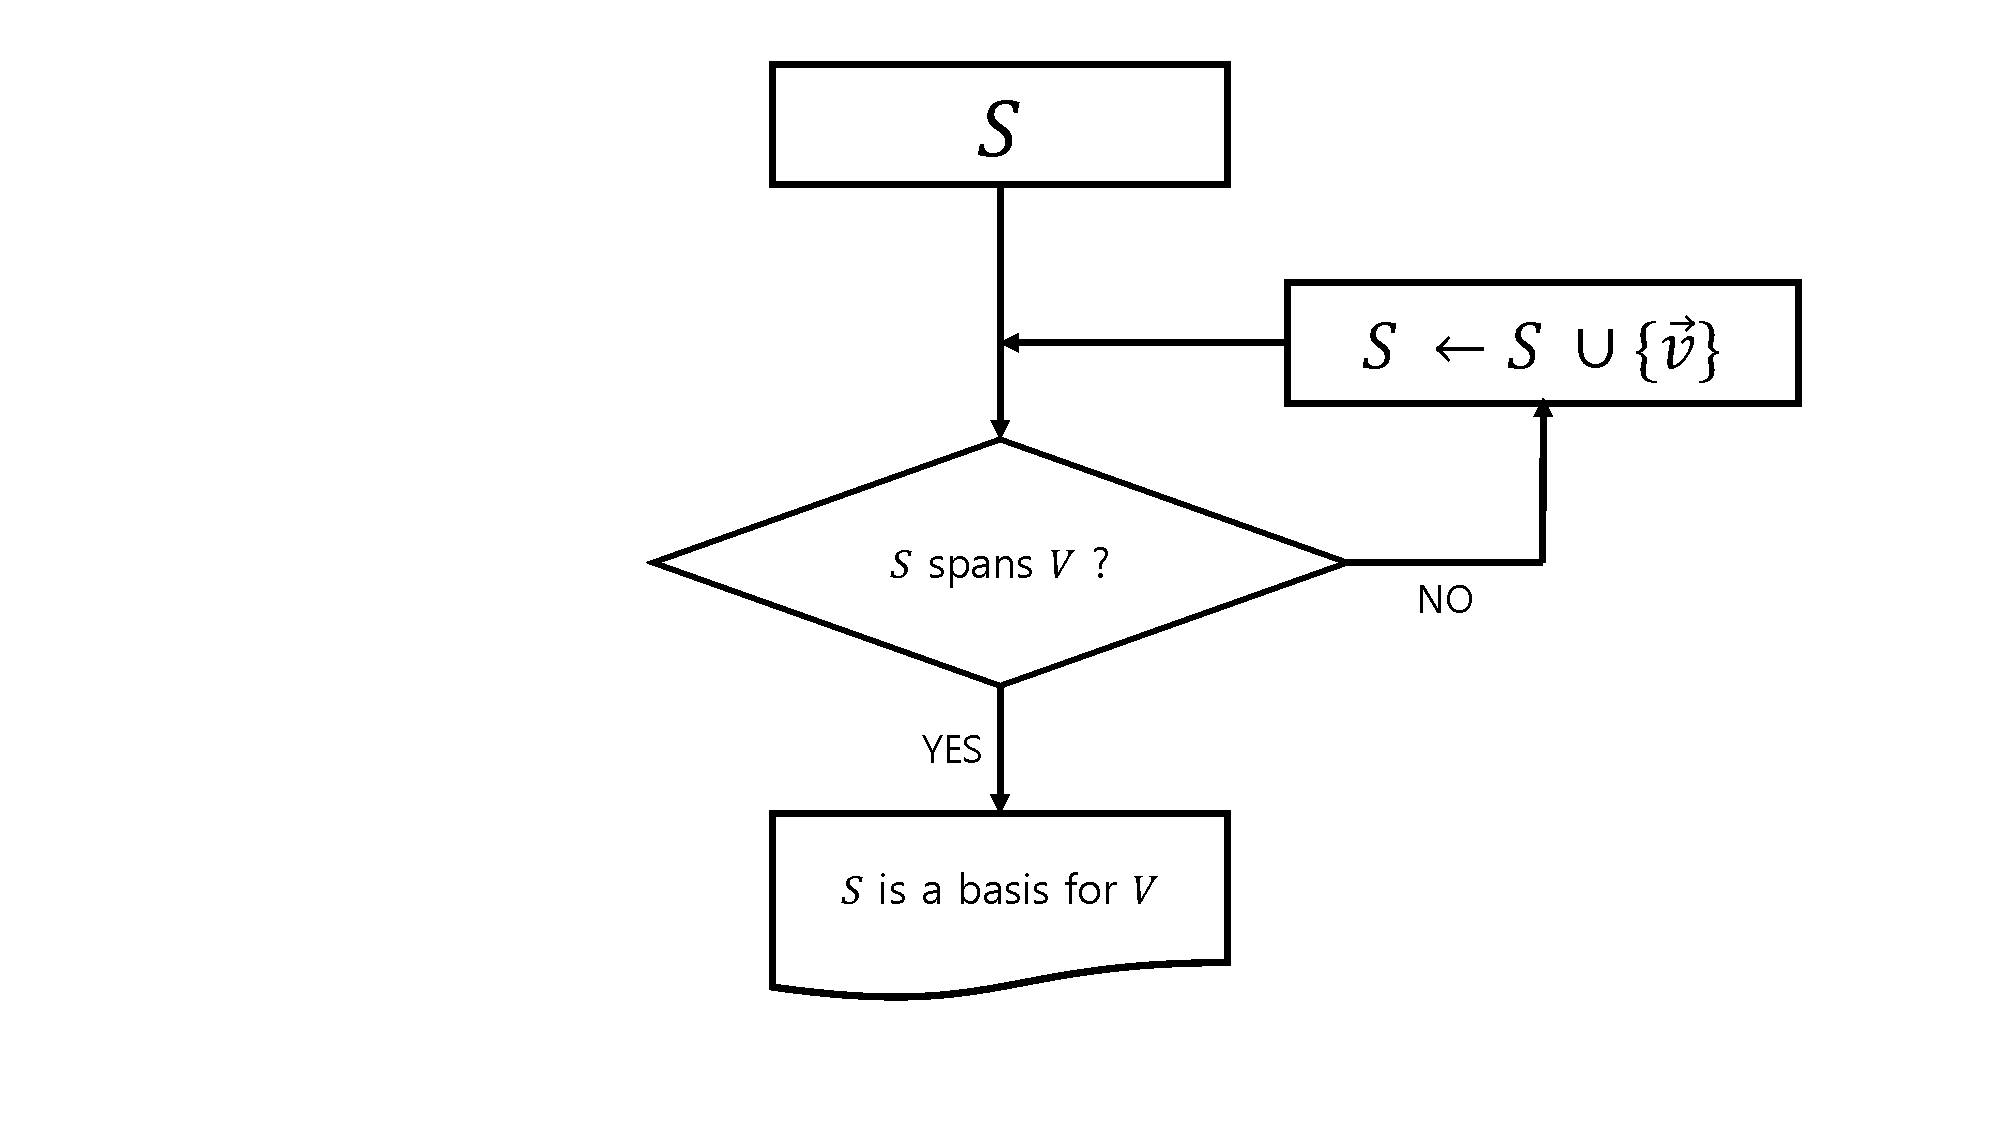
\includegraphics[scale = 0.3]{PlusTheorem.pdf}
			\end{center}
		\end{figure}
		This process terminates in finite operations since a linearly independent set in $V$ has at most $n$ vectors. The final $S$ forms a basis for $V$.
		\item \textbf{(Exercise 6.2 56)} Let $S$ be a spanning set for $V$. If $S$ is not linearly independent, there exist $\textbf{v} \in S$ which can be expressed as the linear combination of the other vectors. Redefine $S = S - \{\textbf{v}\}$, then $S$ is still a spanning set for $V$. (Exercise 6.2 55) Repeat the process until $S$ becomes a linearly independent set in $V$.
		\begin{figure}[H]
			\begin{center}
				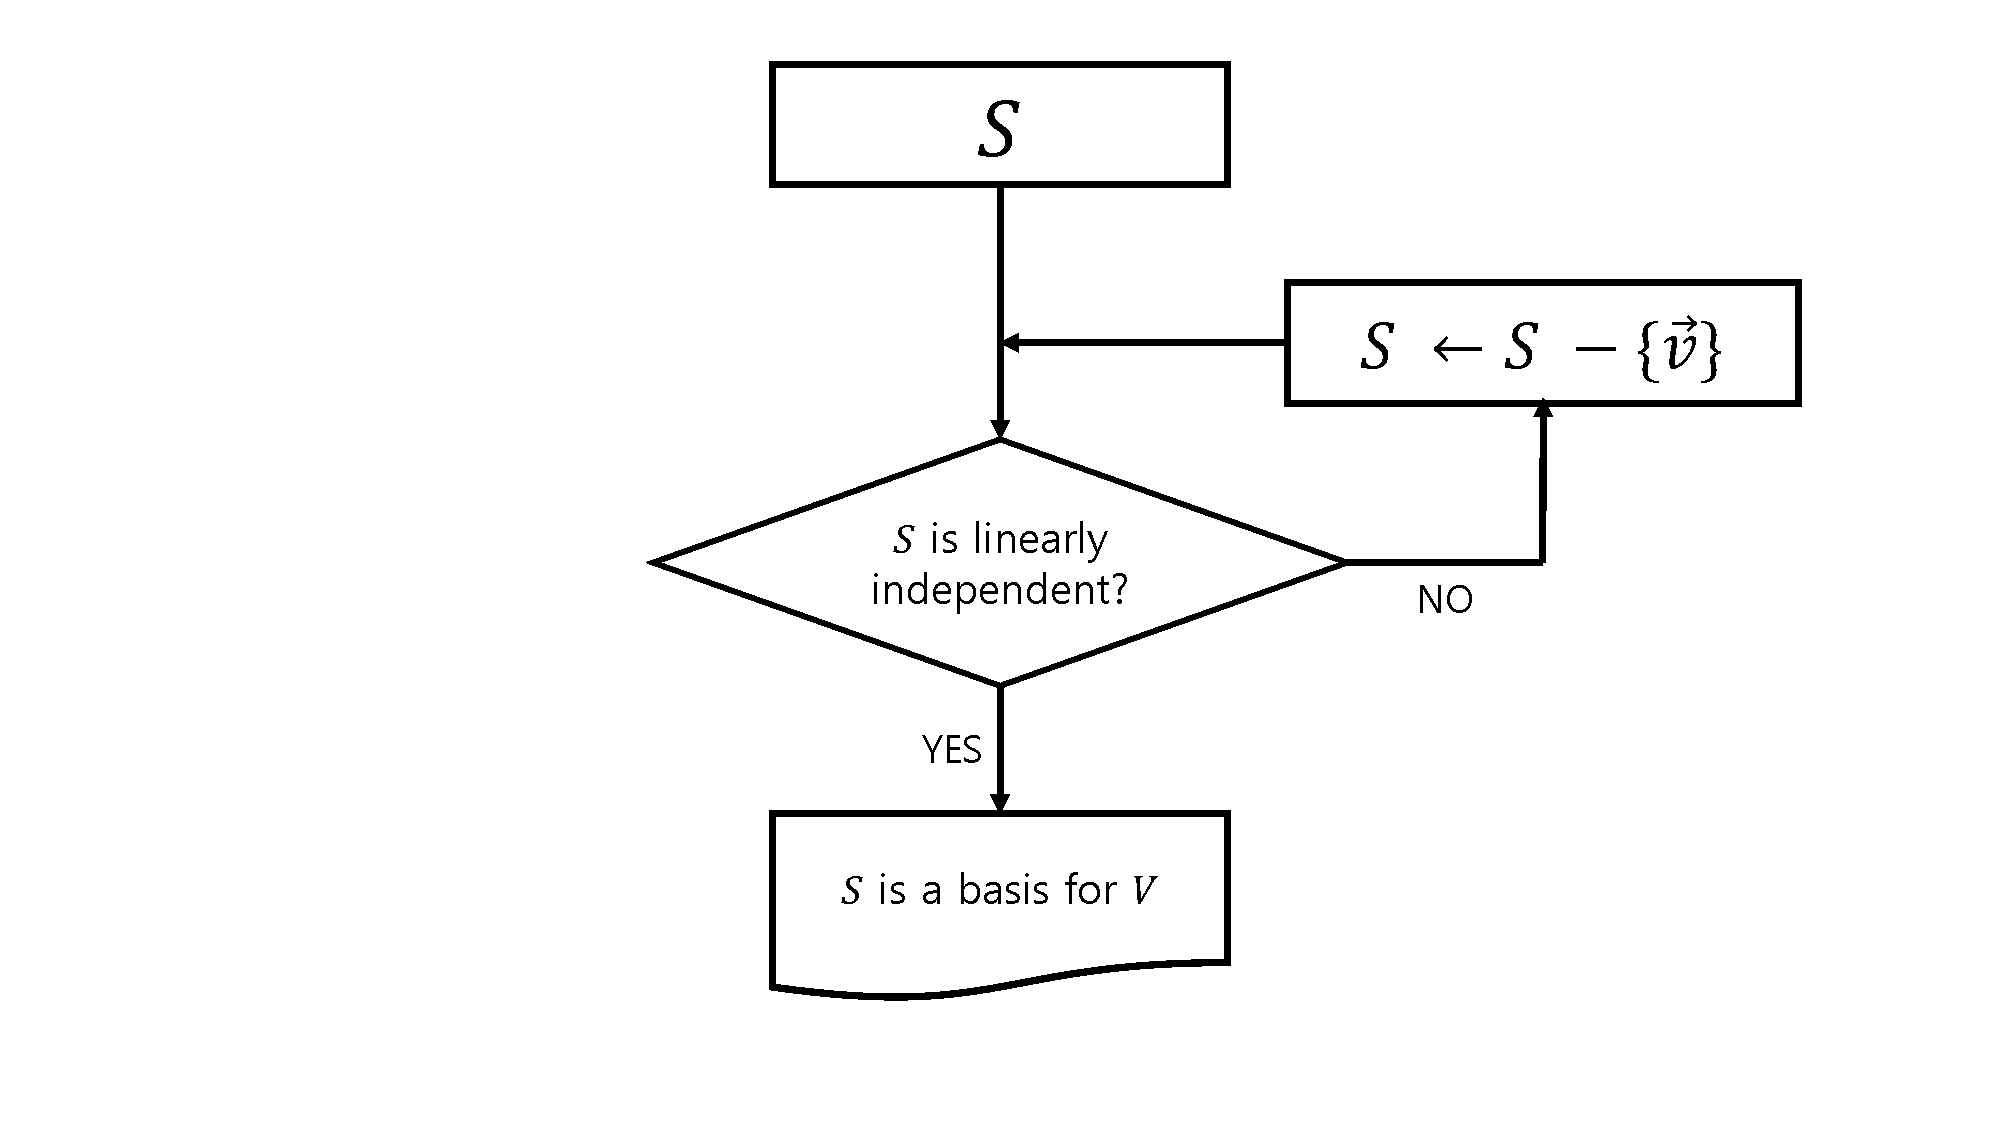
\includegraphics[scale = 0.3]{MinusTheorem.pdf}
			\end{center}
		\end{figure}
		This process terminates in finite operations since a spanning set for $V$ has at least $n$ vectors. The final $S$ forms a basis for $V$.
	\end{enumerate}
\end{proof}

\begin{theorem}
	Let $W$ be a subspace of a finite-dimensional vector space $V$.
	\begin{enumerate}
		\item $W$ is a finite-dimensional and $\dim W \le \dim V$.
		\item $\dim W = \dim V$ if and only if $W = V$.
	\end{enumerate}
\end{theorem}

\begin{proof}
	If $W$ is infinite-dimensional, it contains a infinite set which is linearly independent. However, by Theorem 6.10(a), a linearly independent set in $V$ has at most $n$ vectors. Thus $W$ is finite-dimensional, so let $\mathcal{B}$ be a basis for $W$.
	\begin{enumerate}
		\item (i) If $W = \{ \textbf{0} \}$, then $\dim W = 0 \le \dim V$. \\
		
		(ii) Suppose that $W$ is a nonzero subspace. Since $\mathcal{B}$ is a linearly independent set in $V$, by Theorem 6.10(e), $\mathcal{B}$ can be extended to a basis for $V$, which has $n$ vectors. Therefore, a basis for $W$ has lesser or equal than $n$ vectors, hence $\dim W \le n = \dim V$.
		\item ($\Rightarrow$) If $\dim W = \dim V = n$, then any basis $\mathcal{B}$ consists of $n$ vectors. Since $\mathcal{B}$ is a linearly independent set of $n$ vectors in $V$, it also forms a basis for $V$ by Theorem 6.10(c). Therefore, $V = W$.  \\
		
		($\Leftarrow$) If $W = V$, clearly $\dim W = \dim V$.
	\end{enumerate}
\end{proof}

\newpage
\section{Change of Basis}

6.3, 6.4, 6.5, 6.6 보기 전에 그림을 한 번 보고 가자.

\begin{figure}[H]
	\begin{center}
		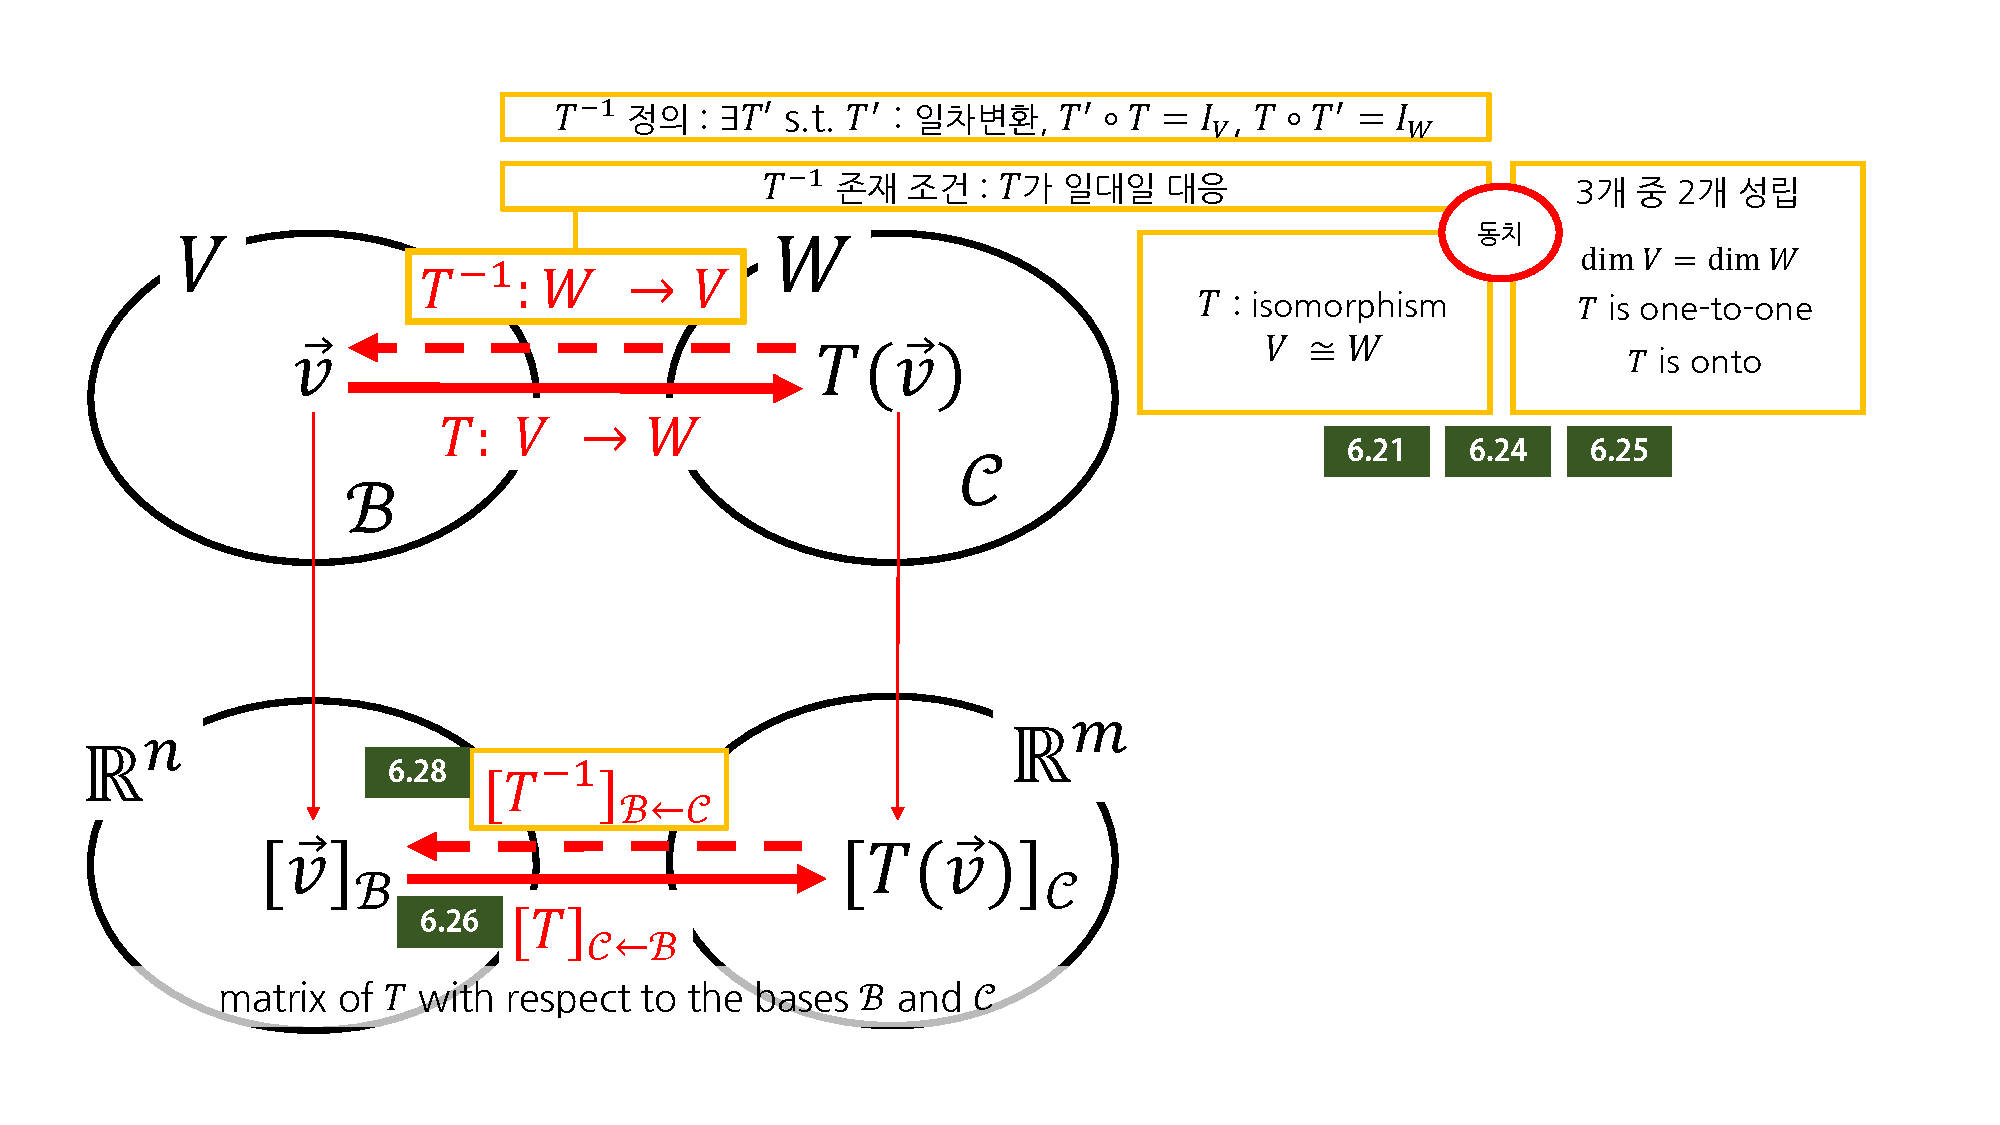
\includegraphics[scale = 0.5]{Figure1.pdf}
	\end{center}
\end{figure}

\begin{figure}[H]
	\begin{center}
		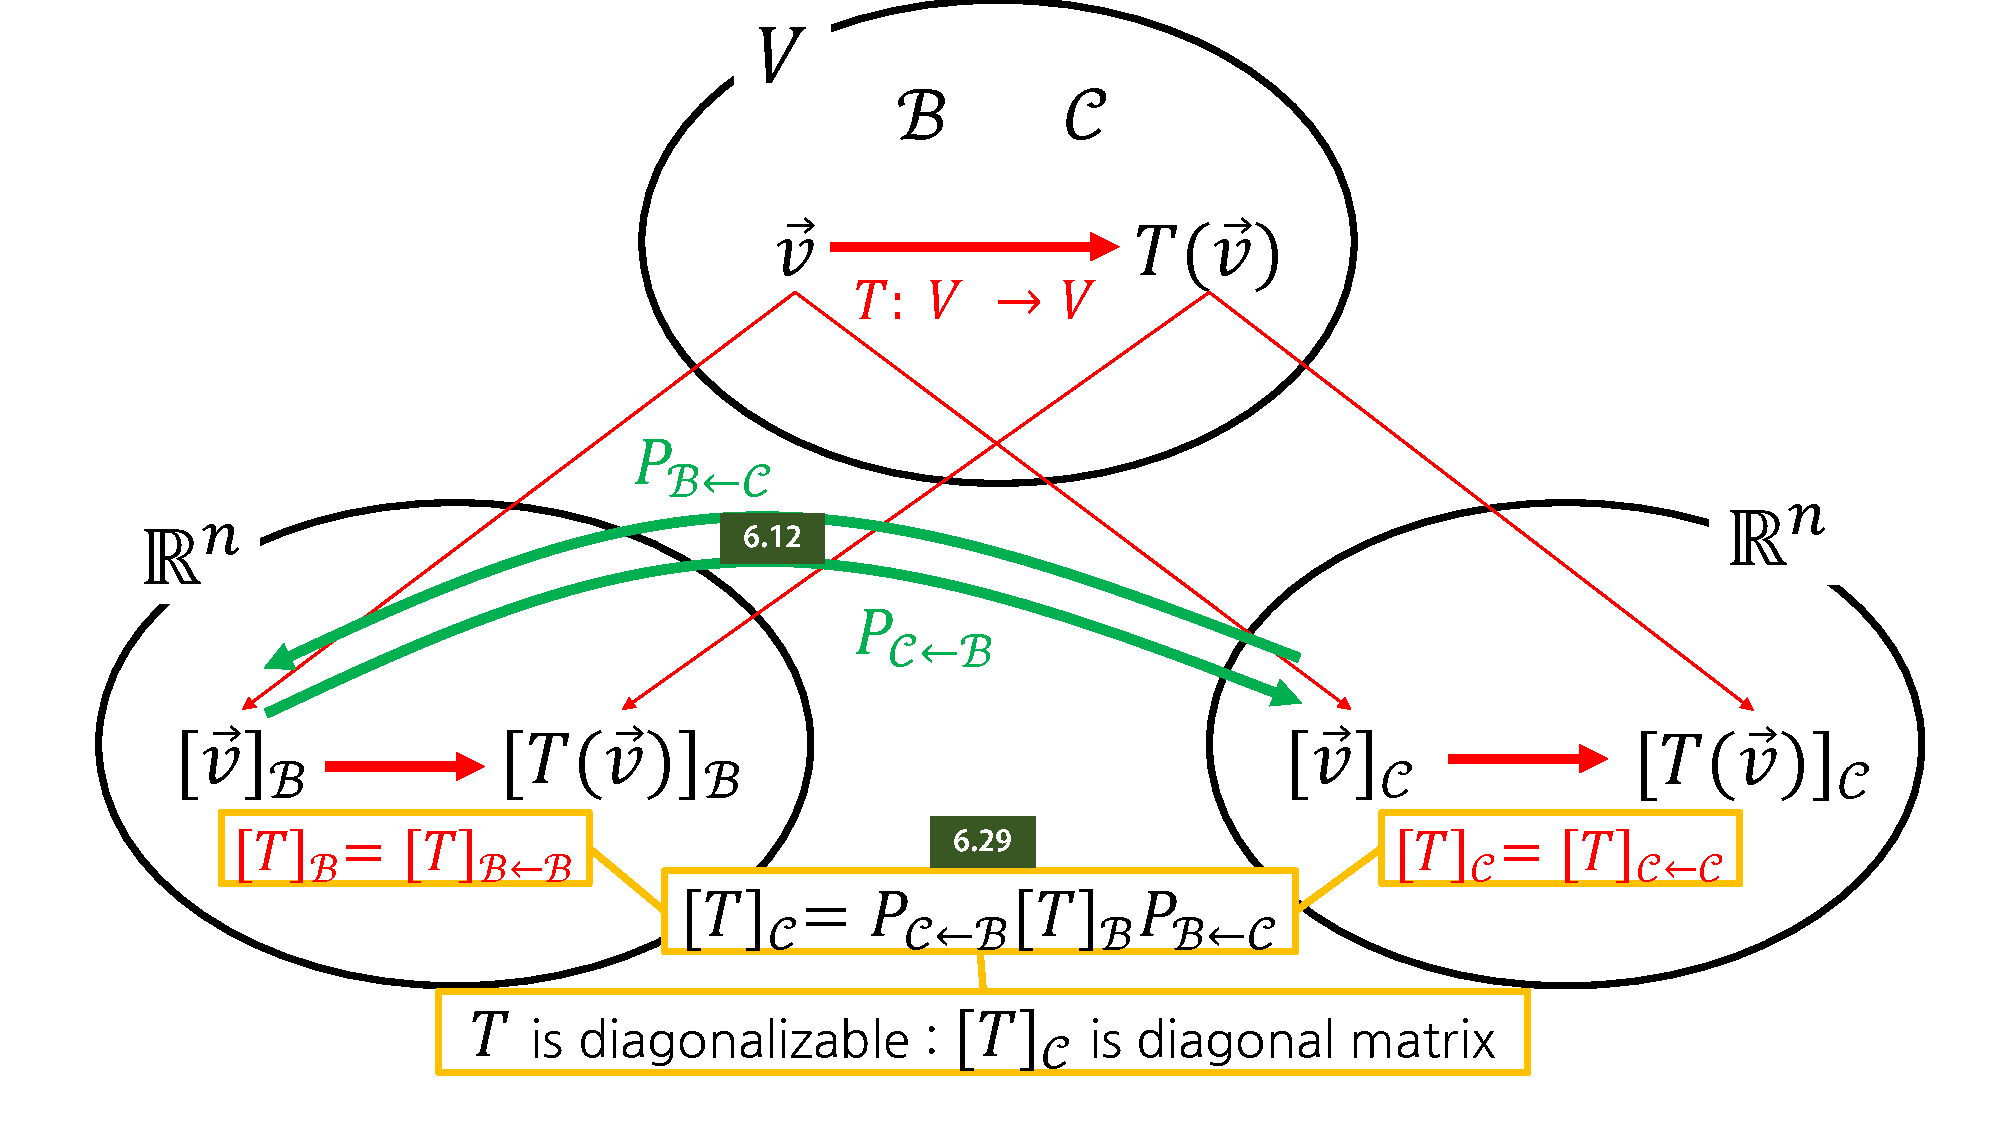
\includegraphics[scale = 0.4]{Figure2.pdf}
	\end{center}
\end{figure}

\newpage
\textit{Definition.} Let $\mathcal{B} = \{ \textbf{u}_1, \cdots, \textbf{u}_n \}$ and $\mathcal{C} = \{ \textbf{v}_1, \cdots, \textbf{v}_n \}$ be bases for a vector space $V$. The $n \times n$ matrix whose columns are the coordinate vectors $[\textbf{u}_1]_\mathcal{C}, \cdots, [\textbf{u}_n]_\mathcal{C}$ is denoted by $P_{\mathcal{C} \leftarrow \mathcal{B}}$ and is called the \textbf{change-of-basis matrix} from $\mathcal{B}$ to $\mathcal{C}$. \begin{equation*}
	P_{\mathcal{C} \leftarrow \mathcal{B}} = \begin{bmatrix}
		\left [ \textbf{u}_1 \right ]_\mathcal{C} & \cdots & \left [ \textbf{u}_n \right ]_\mathcal{C}
	\end{bmatrix}
\end{equation*}

\begin{theorem}
	Let $\mathcal{B} = \{ \textbf{u}_1, \cdots, \textbf{u}_n \}$ and $\mathcal{C} = \{ \textbf{v}_1, \cdots, \textbf{v}_n \}$ be bases for a vector space $V$.
	\begin{enumerate}
		\item $P_{\mathcal{C} \leftarrow \mathcal{B}}[\textbf{x}]_\mathcal{B} = [\textbf{x}]_\mathcal{C}$ for all $\textbf{x} \in V$.
		\item $P_{ \mathcal{C} \leftarrow \mathcal{B} }$ is the unique matrix $P$ with the property that $P[\textbf{x}]_\mathcal{B} = [\textbf{x}]_\mathcal{C}$ for all $\textbf{x} \in V$.
		\item $P_{ \mathcal{C} \leftarrow \mathcal{B} }$ is invertible and $\inv{(P_{ \mathcal{C} \leftarrow \mathcal{B} })} = P_{ \mathcal{B} \leftarrow \mathcal{C} }$.
	\end{enumerate}
\end{theorem}

\begin{proof}
	Let $\mathcal{B} = \{ \textbf{u}_1, \cdots, \textbf{u}_n \}$ and $\mathcal{C} = \{ \textbf{v}_1, \cdots, \textbf{v}_n \}$ be bases for a vector space $V$.
	\begin{enumerate}
		\item Let $\textbf{x}$ be a vector in $V$. Then there exist scalars $c_1, \cdots, c_n$ such that \begin{equation*}
		\textbf{x} = c_1\textbf{u}_1 + \cdots + c_n\textbf{u}_n
		\end{equation*} which implies that \begin{equation*}
		[\textbf{x}]_\mathcal{B} = \begin{bmatrix}
		c_1 \\ \vdots \\ c_n
		\end{bmatrix}
		\end{equation*} Then \begin{align*}
		[\textbf{x}]_\mathcal{C} &= [c_1\textbf{u}_1 + \cdots + c_n\textbf{u}_n]_\mathcal{C} \\
		&= c_1[\textbf{u}_1]_\mathcal{C} + \cdots + c_n[\textbf{u}_n]_\mathcal{C} \\
		&= \begin{bmatrix}
		\left[\textbf{u}_1\right]_\mathcal{C} & \cdots & [\textbf{u}_n]_\mathcal{C}
		\end{bmatrix} \begin{bmatrix}
		c_1 \\ \vdots \\ c_n
		\end{bmatrix} = P_{ \mathcal{C} \leftarrow \mathcal{B} }[\textbf{x}]_\mathcal{B}
		\end{align*}
		\item Suppose that $P = \begin{bmatrix}
			\textbf{p}_1 & \cdots & \textbf{p}_n
		\end{bmatrix}$ is an $n \times n$ matrix such that $P[\textbf{x}]_\mathcal{B} = [\textbf{x}]_\mathcal{C}$ for all $\textbf{x} \in V$. Since $[\textbf{u}_i]_\mathcal{B} = \textbf{e}_i$, for $i = 1, 2, \cdots, n$, \begin{equation*}
			\textbf{p}_i = P\textbf{e}_i = P[\textbf{u}_i]_\mathcal{B} = [\textbf{u}_i]_\mathcal{C}
		\end{equation*} Therefore, \begin{equation*}
			P = \begin{bmatrix}
				\textbf{p}_1 & \cdots & \textbf{p}_n
			\end{bmatrix} = \begin{bmatrix}
				\left[\textbf{u}_1\right]_\mathcal{C} & \cdots & [\textbf{u}_n]_\mathcal{C}
			\end{bmatrix} = P_{ \mathcal{C} \leftarrow \mathcal{B} }
		\end{equation*}
		\item Since $\mathcal{B}$ is a linearly independent set in $V$, the columns of $P_{ \mathcal{C} \leftarrow \mathcal{B} }$ are also linearly independent in $\mathbb{R}^n$ by Theorem 6.7, so $P_{ \mathcal{C} \leftarrow \mathcal{B} }$ is invertible by F.T.I.M. Since $P_{ \mathcal{C} \leftarrow \mathcal{B} }$ is invertible, for every $\textbf{x}$ in $V$, $[\textbf{x}]_\mathcal{B} = \inv{(P_{ \mathcal{C} \leftarrow \mathcal{B} })}[\textbf{x}]_\mathcal{C}$. Therefore, by Theorem 6.12(b), $\inv{(P_{ \mathcal{C} \leftarrow \mathcal{B} })} = P_{ \mathcal{B} \leftarrow \mathcal{C} }$. 
	\end{enumerate}
\end{proof}

\begin{theorem}
	Let $\mathcal{B} = \{ \textbf{u}_1, \cdots, \textbf{u}_n \}$ and $\mathcal{C} = \{ \textbf{v}_1, \cdots, \textbf{v}_n \}$ are basis for a vector space $V$. Let $B = \begin{bmatrix}
		\left[ \textbf{u}_1 \right]_\mathcal{E} & \cdots & \left[ \textbf{u}_n \right]_\mathcal{E}
	\end{bmatrix}$ and $C = \begin{bmatrix}
	\left[ \textbf{v}_1 \right]_\mathcal{E} & \cdots & \left[ \textbf{v}_n \right]_\mathcal{E}
	\end{bmatrix}$, where $\mathcal{E}$ is any basis for $V$. Then the row reduction applied to $n \times 2n$ augmented matrix $\begin{bmatrix} [c|c]
		C & B
	\end{bmatrix}$ produces \begin{equation*}
		\begin{bmatrix} [c|c]
		C & B
		\end{bmatrix} \rightarrow \begin{bmatrix} [c|c]
		I & P_{\mathcal{C} \leftarrow \mathcal{B}}
		\end{bmatrix}
	\end{equation*}
\end{theorem}

\begin{proof}
	Let scalars $p_{ij}$ such that \begin{equation*}
		[\textbf{u}_i]_\mathcal{C} = \begin{bmatrix}
			p_{1i} \\ \vdots \\ p_{ni}
		\end{bmatrix} \mbox{ for } i = 1, 2, \cdots, n
	\end{equation*} Then \begin{equation*}
		P_{ \mathcal{C} \leftarrow \mathcal{B} } = \begin{bmatrix}
			\left [\textbf{u}_1\right ]_\mathcal{C} & \cdots & [\textbf{u}_n]_\mathcal{C}
		\end{bmatrix} = \begin{bmatrix}
			p_{11} & \cdots & p_{1n} \\
			\vdots & & \vdots \\
			p_{n1} & \cdots & p_{nn}
		\end{bmatrix}
	\end{equation*}
	Let $\mathcal{E}$ be a basis for $V$. Since $\textbf{u}_i = p_{1i}\textbf{v}_1 + \cdots + p_{ni}\textbf{v}_n$, for $i = 1, 2, \cdots, n$, \begin{align*}
		[\textbf{u}_i]_\mathcal{E} &= [p_{1i}\textbf{v}_1 + \cdots + p_{ni}\textbf{v}_n]_\mathcal{E} = p_{1i}[\textbf{v}_1]_\mathcal{E} + \cdots + p_{ni}[\textbf{v}_n]_\mathcal{E} \\
		&= \begin{bmatrix}
			\left[\textbf{v}_1\right]_\mathcal{E} & \cdots & \left[\textbf{v}_n\right]_\mathcal{E}
		\end{bmatrix}\begin{bmatrix}
			p_{1i} \\ \vdots \\ p_{ni}
		\end{bmatrix}
	\end{align*}
	Thus, $\begin{bmatrix}
		p_{1i} \\ \vdots \\ p_{ni}
	\end{bmatrix}$ is the solution of the linear system with the augmented matrix given as \begin{equation*}
		\begin{bmatrix}[ccc|c]
			\left[\textbf{v}_1\right]_\mathcal{E} & \cdots & \left[\textbf{v}_n\right]_\mathcal{E} & \left[\textbf{u}_i\right]_\mathcal{E}
		\end{bmatrix}
	\end{equation*}
	Since the coefficient matrix is equal for each $i = 1, 2, \cdots, n$, $P$ can be obtained by row reducing the $n \times 2n$ augmented matrix \begin{equation*}
		\begin{bmatrix}[ccc|ccc]
			\left[\textbf{v}_1\right]_\mathcal{E} & \cdots & \left[\textbf{v}_n\right]_\mathcal{E} & \left[\textbf{u}_1\right]_\mathcal{E} & \cdots & \left[\textbf{u}_n\right]_\mathcal{E}
		\end{bmatrix} = \begin{bmatrix}[c|c]
		C & B
		\end{bmatrix}
	\end{equation*}
	Since $\textbf{v}_1, \cdots, \textbf{v}_n$ are linearly independent, $\left[\textbf{v}_1\right]_\mathcal{E}, \cdots , \left[\textbf{v}_n\right]_\mathcal{E}$ are also linearly independent by Theorem 6.7. Thus, by F.T.I.M, RREF of $C$ is $I$. Therefore, row reducing the augmented matrix will result in \begin{equation*}
		\begin{bmatrix}[c|c]
		C & B
		\end{bmatrix} \rightarrow \begin{bmatrix}[c|c]
		I & P_{ \mathcal{C} \leftarrow \mathcal{B} }
		\end{bmatrix}
	\end{equation*}
\end{proof}

% 3.6 추가할 것. %
\section{Linear Transformations + 3.6 Part I}

\textit{Definition.} A \textbf{linear transformation} from a vector space $V$ to a vector space $W$ is a mapping $T: V \rightarrow W$ such that for all $\textbf{u}$ and $\textbf{v}$ in $V$ and for all scalars $c$, \begin{enumerate}
	\item $T(\textbf{u} + \textbf{v}) = T(\textbf{u}) + T(\textbf{v})$
	\item $T(c\textbf{u}) = cT(\textbf{u})$
\end{enumerate}

\begin{theorem}
	Let $T: V \rightarrow W$ be a linear transformation. \begin{enumerate}
		\item $T(\textbf{0}) = \textbf{0}$
		\item $T(-\textbf{v}) = -T(\textbf{v})$ for all $\textbf{v} \in V$
		\item $T(\textbf{u} - \textbf{v}) = T(\textbf{u}) - T(\textbf{v})$ for all $\textbf{u}, \textbf{v} \in V$
	\end{enumerate}
\end{theorem}

\begin{proof}
	Let $T: V \rightarrow W$ be a linear transformation.
	\begin{enumerate}
		\item Let $\textbf{v}$ be a vector in $V$. Then \begin{align*}
			T(\textbf{0}) = T(0\textbf{v}) = 0T(\textbf{v}) = \textbf{0}
		\end{align*}
		\item \textbf{(Exercise 6.4 21)} For any $\textbf{v} \in V$, \begin{equation*}
			T(-\textbf{v}) = T((-1)\textbf{v}) = (-1)T(\textbf{v}) = -T(\textbf{v})
		\end{equation*}
		\item For any $\textbf{u}, \textbf{v} \in V$, \begin{equation*}
			T(\textbf{u} - \textbf{v}) = T(\textbf{u} + (-1)\textbf{v}) = T(\textbf{u}) + (-1)T(\textbf{v}) = T(\textbf{u}) - T(\textbf{v})
		\end{equation*}
	\end{enumerate}
\end{proof}

\textit{Note.} Theorem 6.14(a)에서 $V$의 zero vector와 $W$의 zero vector를 잘 구분하자.

\begin{theorem}
	Let $T: V \rightarrow W$ be a linear transformation and let $\mathcal{B} = \{ \textbf{v}_1, \cdots, \textbf{v}_n \}$ is a spanning set for $V$. Then $T(\mathcal{B}) = \{ T(\textbf{v}_1), \cdots, T(\textbf{v}_n) \}$ is the spanning set for range of $T$.
\end{theorem}

\begin{proof}
	Let $\textbf{w}$ be a vector in range($T$), then there exists a vector $\textbf{v} \in V$ such that $\textbf{w} = T(\textbf{v})$. Since $\mathcal{B}$ spans $V$, there exist scalars $c_1, \cdots, c_n$ such that \begin{equation*}
		\textbf{v} = c_1\textbf{v}_1 + \cdots + c_n\textbf{v}_n
	\end{equation*} Thus, \begin{equation*}
		\textbf{w} = T(\textbf{v}) = T(c_1\textbf{v}_1 + \cdots + c_n\textbf{v}_n) = c_1T(\textbf{v}_1) + \cdots + c_nT(\textbf{v}_n)
	\end{equation*} Therefore, $\textbf{w}$ is in span($T(\mathcal{B})$), hence $T(\mathcal{B})$ is a spanning set for range($T$).
\end{proof}

\textit{Note.} Spanning set은 이렇게 되는데, linear independence는 $T$가 one-to-one이어야 성립한다. (Theorem 6.22) \\

\textit{Definition.} If $T: U \rightarrow V$ and $S: V \rightarrow W$ are linear transformations, then the \textbf{composition of S with T} is the mapping $S \circ T$, defined by \begin{equation*}
	(S \circ T)(\textbf{u}) = S(T(\textbf{u}))
\end{equation*}

\begin{theorem}
	If $T: U \rightarrow V$ and $S: V \rightarrow W$ are linear transformations, then $S \circ T: U \rightarrow W$ is a linear transformation.
\end{theorem}

\textbf{Theorem 3.32 : Part 1} \\
 Let $T: \mathbb{R}^m \rightarrow \mathbb{R}^n$ and $S: \mathbb{R}^n \rightarrow \mathbb{R}^p$ be linear transformations. Then $S \circ T: \mathbb{R}^m \rightarrow \mathbb{R}^p$ is a linear transformation. \\

\begin{proof}
	Let $\textbf{u}, \textbf{v}$ be vectors in $U$, and let $c$ be a scalar. Then \begin{align*}
		(S \circ T)(\textbf{u} + \textbf{v}) &= S(T(\textbf{u} + \textbf{v})) \\
		&= S(T(\textbf{u}) + T(\textbf{v}) \\
		&= S(T(\textbf{u})) + S(T(\textbf{v})) = (S \circ T)(\textbf{u}) + (S \circ T)(\textbf{v})
	\end{align*}
	Also, \begin{align*}
		(S \circ T)(c\textbf{u}) &= S(T(c\textbf{u})) \\
		&= S(cT(\textbf{u})) \\
		&= cS(T(\textbf{u})) = c(S \circ T)(\textbf{u})
	\end{align*}
	Therefore, $S \cdot T$ is a linear transformation.
\end{proof}

\textit{Definition.} A linear transformation $T: V \rightarrow W$ is \textbf{invertible} if there exists a linear transformation $T': W \rightarrow V$ such that \begin{equation*}
	T' \circ T = I_V \mbox{ and } T \circ T' = I_W
\end{equation*} and such linear transformation $T'$ is called an \textbf{inverse} for $T$.

\begin{theorem}
	If $T$ is an invertible linear transformation, then its inverse is unique.
\end{theorem}

\begin{proof}
	\textbf{(Exercise 6.4 31)} Let $T: V \rightarrow W$ be an invertible linear transformation. Suppose that $T': W \rightarrow V$ and $T'': W \rightarrow V$ are both inverses of $T$, then \begin{align*}
		T \circ T' = T \circ T'' = I_W \mbox{ and } T' \circ T = T'' \circ T = I_V
	\end{align*} Thus, \begin{align*}
		T' = I_V \circ T' = (T'' \circ T) \circ T' = T'' \circ (T \circ T') = T'' \circ I_W = T''
	\end{align*} Therefore, the inverse of $T$ is unique.
\end{proof}

\section{Kernel and Range}
\textit{Definition.} Let $T: V \rightarrow W$ be a linear transformation. The \textbf{kernel} of $T$, denoted by ker($T$), is defined by \begin{equation*}
	\textnormal{ker}(T) = \{ \textbf{v} \in V \vert T(\textbf{v}) = \textbf{0} \}
\end{equation*}
The \textbf{range} of $T$, denoted by range($T$), is defined by \begin{equation*}
	\textnormal{range}(T) = \{\textbf{w} \in W \vert \textbf{w} = T(\textbf{v}) \mbox{ for some } \textbf{v} \in V \}
\end{equation*}

\textit{Note.} ker($T$)는 $V$의 vector들의 집합이고, range($T$)는 $W$의 vector들의 집합임을 상기하자.

\begin{theorem}
	Let $T: V \rightarrow W$ be a linear transformation. \begin{enumerate}
		\item ker($T$) is a subspace of $V$.
		\item range($T$) is a subspace of $W$.
	\end{enumerate}
\end{theorem}

\begin{proof}
	Let $T: V \rightarrow W$ be a linear transformation.
	\begin{enumerate}
		\item Since $T(\textbf{0}) = \textbf{0}$ by Theorem 6.14(a), $\textbf{0} \in \ker(T)$ so ker($T$) is a nonempty set. Let $\textbf{u}, \textbf{v}$ be vectors in ker($T$), and let $c$ be a scalar, then \begin{align*}
			&T(\textbf{u} + \textbf{v}) = T(\textbf{u}) + T(\textbf{v}) = \textbf{0} + \textbf{0} = \textbf{0} \\
			&T(c\textbf{u}) = cT(\textbf{u}) = c\textbf{0} = \textbf{0}
		\end{align*} Therefore $\textbf{u} + \textbf{v} \in \ker(T)$ and $c\textbf{u} \in \ker(T)$, hence ker($T$) is a subspace of $V$ by Theorem 6.2.
		\item Since $T(\textbf{0}) = \textbf{0}$ by Theorem 6.14(a), $\textbf{0} \in$ range($T$) so range($T$) is a nonempty set. Let $\textbf{w}_1, \textbf{w}_2$ be vectors in range($T$) and let $c$ be a scalar. Then there exist $\textbf{v}_1, \textbf{v}_2 \in V$ such that $T(\textbf{v}_1) = \textbf{w}_1$ and $ T(\textbf{v}_2) = \textbf{w}_2$. Then \begin{align*}
			&\textbf{w}_1 + \textbf{w}_2 = T(\textbf{v}_1) + T(\textbf{v}_2) = T(\textbf{v}_1 + \textbf{v}_2) \\
			&c\textbf{w}_1 = cT(\textbf{v}_1) = T(c\textbf{v}_1)
		\end{align*} Therefore $\textbf{w}_1 + \textbf{w}_2 \in$ range($T$) and $c\textbf{w}_1 \in $ range($T$), hence range($T$) is a subspace of $V$ by Theorem 6.2.
	\end{enumerate}
\end{proof}

이제 ker($T$)와 range($T$)가 vector space임을 증명했으니 그 dimension으로 rank와 nullity를 정의할 수 있다. \\

\textit{Definition.} Let $T: V \rightarrow W$ be a linear transformation. Then the rank and nullity of $T$, denoted by rank($T$) and nullity($T$), is defined by \begin{equation*}
	\textnormal{rank}(T) = \dim(\textnormal{range}(T)) \mbox{ and } \textnormal{nullity}(T) = \dim(\ker{(T)})
\end{equation*}

\begin{theorem}[The Rank Theorem : for Linear Transformation]
	Let $T: V \rightarrow W$ be a linear transformation from a finite-dimensional vector space $V$ to a vector space $W$. Then \begin{equation*}
		\textnormal{rank}(T) + \textnormal{nullity}(T) = \dim V
	\end{equation*}
\end{theorem}

\begin{proof}
	Let $n = \dim V$, and let $\{ \textbf{v}_1, \cdots, \textbf{v}_k \}$ be a basis for ker($T$). By Theorem 6.10(e), $\{ \textbf{v}_1, \cdots, \textbf{v}_k \}$ can be extended to a basis $\mathcal{B} = \{ \textbf{v}_1, \cdots, \textbf{v}_k, \textbf{v}_{k+1}, \cdots, \textbf{v}_n \}$ for $V$. \\
	
	Let $\mathcal{C} = \{ T(\textbf{v}_{k+1}), \cdots, T(\textbf{v}_n) \}$, then $\mathcal{C}$ is a subset of range($T$). Let $\textbf{w}$ be a vector in range($T$), then there exists $\textbf{v} \in V$ such that $T(\textbf{v}) = \textbf{w}$. Then there exist scalars $c_1, \cdots, c_n$ such that \begin{equation*}
		\textbf{v} = c_1\textbf{v}_1 + \cdots + c_k\textbf{v}_k + c_{k+1}\textbf{v}_{k+1} + \cdots + c_n\textbf{v}_n
	\end{equation*} Then \begin{align*}
		\textbf{w} = T(\textbf{v}) &= T(c_1\textbf{v}_1 + \cdots + c_k\textbf{v}_k + c_{k+1}\textbf{v}_{k+1} + \cdots + c_n\textbf{v}_n) \\
		&= c_1T(\textbf{v}_1) + \cdots + c_kT(\textbf{v}_k) + c_{k+1}T(\textbf{v}_{k+1}) + \cdots + c_nT(\textbf{v}_n) \\
		&= c_{k+1}T(\textbf{v}_{k+1}) + \cdots + c_nT(\textbf{v}_n)
	\end{align*} Thus $\textbf{w} \in $ span($\mathcal{C}$), which implies that $\mathcal{C}$ is a spanning set for range($T$). \\
	
	Now, consider the equation \begin{equation*}
		c_{k+1}T(\textbf{v}_{k+1}) + \cdots + c_nT(\textbf{v}_n) = \textbf{0}
	\end{equation*} Then $T(c_{k+1}\textbf{v}_{k+1} + \cdots + c_n\textbf{v}_n) = \textbf{0}$, so $c_{k+1}\textbf{v}_{k+1} + \cdots + c_n\textbf{v}_n \in \ker(T)$. Since $\mathcal{B}$ is a basis for $\ker(T)$, there exist scalars $c_1, \cdots, c_k$ such that \begin{equation*}
		c_{k+1}\textbf{v}_{k+1} + \cdots + c_n\textbf{v}_n = c_1\textbf{v}_1 + \cdots + c_k\textbf{v}_k
	\end{equation*} Since $\textbf{v}_1, \cdots, \textbf{v}_n$ are linearly independent, this implies that $c_1 = \cdots = c_k = c_{k+1} = \cdots = c_n = 0$. Therefore, $T(\textbf{v}_{k+1}), \cdots, T(\textbf{v}_n)$ are linearly independent. \\
	
	Since $\mathcal{C}$ is linearly independent and is a spanning set for range($T$), it forms a basis for range($T$). Therefore, \begin{equation*}
		\textnormal{rank}(T) + \textnormal{nullity}(T) = (n - k) + k = n = \dim V
	\end{equation*}
\end{proof}

\textit{Definition.} A linear transformation $T: V \rightarrow W$ is called \textbf{one-to-one} if $T$ maps distinct vectors in $V$ to distinct vectors in $W$. That is, for vectors $\textbf{v}, \textbf{w}$ in $V$, \begin{equation*}
	\textbf{v} \neq \textbf{w} \Rightarrow T(\textbf{v}) \neq T(\textbf{w})
\end{equation*}

\textit{Definition.} A linear transformation $T: V \rightarrow W$ is called \textbf{onto} if range($T$) = $W$. That is, \begin{equation*}
	^\forall \textbf{w} \in W, ^\exists \textbf{v} \in V \mbox{ such that } T(\textbf{v}) = \textbf{w}
\end{equation*}

\begin{theorem}
	A linear transformation $T: V \rightarrow W$ is one-to-one if and only if ker($T$) = $\{ \textbf{0} \}$.
\end{theorem}

\begin{proof}
	($\Rightarrow$) Suppose that there exists a nonzero vector $\textbf{v}$ in ker($T$). Then $T(\textbf{v}) = T(\textbf{0}) = \textbf{0}$, which is a contradiction since $T$ is one-to-one. Therefore, ker($T$) = $\{ \textbf{0} \}$. \\
	
	($\Leftarrow$) Let $\textbf{u}, \textbf{v} \in V$ such that $T(\textbf{u}) = T(\textbf{v})$. Since ker($T$) = $\{\textbf{0}\}$ and $T(\textbf{u} - \textbf{v}) = T(\textbf{u}) - T(\textbf{v}) = \textbf{0}$, $\textbf{u} - \textbf{v} = \textbf{0}$. Therefore, $\textbf{u} = \textbf{v}$ and hence, $T$ is one-to-one.
\end{proof}

\begin{theorem}
	Let $\dim V = \dim W = n$. Then a linear transformation $T: V \rightarrow W$ is one-to-one if and only if it is onto.
\end{theorem}

\begin{proof}
	($\Rightarrow$) If $T$ is one-to-one, ker($T$) = $\{ \textbf{0} \}$ by Theorem 6.20, so nullity($T$) = 0. By the Rank Theorem, rank($T$) = dim(range($T$)) = 0. Since range($T$) is a subspace of $W$, range($T$) = $W$ by Theorem 6.11(b). Therefore, $T$ is onto. \\
	
	($\Leftarrow$) If $T$ is onto, then rank($T$) = dim(range($T$)) = dim($W$) = $n$. By the Rank Theorem, nullity($T$) = dim(ker($T$)) = 0, so ker($T$) = $\{\textbf{0}\}$. Therefore, by Theorem 6.20, $T$ is one-to-one.
\end{proof}

\begin{theorem}
	Let $T: V \rightarrow W$ be a one-to-one linear transformation. If $S = \{ \textbf{v}_1, \cdots, \textbf{v}_k \}$ is a linearly independent set in $V$, Then $T(S) = \{ T(\textbf{v}_1), \cdots, T(\textbf{v}_k) \}$ is a linearly independent set in $W$.
\end{theorem}
\begin{proof}
	Consider the equation \begin{equation*}
		c_1T(\textbf{v}_1) + \cdots + c_kT(\textbf{v}_k) = \textbf{0}
	\end{equation*} Then $T(c_1\textbf{v}_1 + \cdots + c_k\textbf{v}_k) = \textbf{0}$, so $c_1\textbf{v}_1 + \cdots + c_k\textbf{v}_k \in \ker(T)$. Since $T$ is one-to-one, ker($T$) = $\{\textbf{0}\}$ by Theorem 6.20, so $c_1\textbf{v}_1 + \cdots + c_k\textbf{v}_k = \textbf{0}$. This implies that $c_1 = \cdots = c_k = 0$, since $\textbf{v}_1, \cdots, \textbf{v}_k$ are linearly independent. Therefore, $T(\textbf{v}_1), \cdots, T(\textbf{v}_k)$ are also linearly independent.
\end{proof}

\begin{corollary}
	Let $\dim V = \dim W = n$. Then a one-to-one linear transformation $T: V \rightarrow W$ maps a basis for $V$ to a basis for $W$.
\end{corollary}

\begin{proof}
	If $\mathcal{B}$ is a basis of $V$, Theorem 6.15 and Theorem 6.22 together gives that $T(\mathcal{B})$ is a linearly independent set in $W$ and is a spanning set for $W$. Therefore, $T(\mathcal{B})$ is a basis for $W$.
\end{proof}

\begin{theorem}
	A linear transformation $T: V \rightarrow W$ is invertible if and only if it is one-to-one and onto.
\end{theorem}

\begin{proof}
	($\Rightarrow$) Suppose that $T$ is invertible. Then there exists a linear transformation $\inv{T}: W \rightarrow V$ such that \begin{equation*}
		\inv{T} \circ T = I_V \mbox{ and } T \circ \inv{T} = I_W
	\end{equation*}
	(i) Let $\textbf{v}$ be a vector in ker($T$), then $T(\textbf{v}) = \textbf{0}$. Then, \begin{equation*}
		I_V(\textbf{v}) = (\inv{T} \circ T)(\textbf{v}) = \inv{T}(T(\textbf{v})) = \inv{T}(\textbf{0}) = \textbf{0}
	\end{equation*} Thus, $\textbf{v} = \textbf{0}$, which implies that ker($T$) = $\{\textbf{0}\}$. Therefore, $T$ is one-to-one by Theorem 6.20. \\
	
	(ii) Let $\textbf{w}$ be a vector in $W$, and let $\textbf{v} = \inv{T}(\textbf{w})$. Then \begin{equation*}
		T(\textbf{v}) = T(\inv{T}(\textbf{w})) = (T \circ \inv{T})(\textbf{w}) = I_W(\textbf{w}) = \textbf{w}
	\end{equation*} Therefore, $\textbf{w} \in $ range($T$). Therefore, range($T$) = $W$ and $T$ is onto. \\
	
	($\Leftarrow$) Suppose that $T: V \rightarrow W$ is one-to-one and onto. For every vector $\textbf{w}$ in $W$, there exists a unique vector $\textbf{v} \in V$ such that $T(\textbf{v}) = \textbf{w}$, since $T$ is one-to-one and onto. Let $T': W \rightarrow V$ be a transformation which maps $\textbf{w}$ into such $\textbf{v}$. \\
	
	Let $\textbf{w}_1, \textbf{w}_2$ be vectors in $W$ and $c$ a scalar. Let $\textbf{v}_1, \textbf{v}_2$ be vectors such that $T(\textbf{v}_1) = \textbf{w}_1$ and $T(\textbf{v}_2) = \textbf{w}_2$, then $T'(\textbf{w}_1) = \textbf{v}_1$ and $T'(\textbf{w}_2) = \textbf{v}_2$. Then \begin{align*}
		T(\textbf{v}_1 + \textbf{v}_2) = T(\textbf{v}_1) &+ T(\textbf{v}_2) = \textbf{w}_1 + \textbf{w}_2 \\
		T(c\textbf{v}_1) &= cT(\textbf{v}_1) = c\textbf{w}_1
	\end{align*}
	so $T'(\textbf{w}_1 + \textbf{w}_2) = \textbf{v}_1 + \textbf{v}_2 = T'(\textbf{w}_1) + T'(\textbf{w}_2)$ and $T'(c\textbf{w}_1) = c\textbf{v}_1 = cT(\textbf{w}_1)$. Therefore, $T'$ is a linear transformation. \\
	
	Also, for any vector $\textbf{v} \in V$, let $\textbf{w} = T(\textbf{v})$ then $T'(\textbf{w}) = \textbf{v}$, so \begin{align*}
		(T' \circ T)(\textbf{v}) &= T'(T(\textbf{v})) = T'(\textbf{w}) = \textbf{v} \\
		(T \circ T')(\textbf{w}) &= T(T'(\textbf{w})) = T(\textbf{v}) = \textbf{w}
	\end{align*} This implies that $T' \circ T = I_V$ and $T \circ T' = I_W$. \\
	
	Therefore, $T'$ is an inverse of $T$, hence $T$ is invertible.
\end{proof}

\textit{Definition.} A linear transformation $T: V \rightarrow W$ is called \textbf{isomorphism} if it is one-to-one and onto. If $V$ and $W$ are two vector spaces such that there exists an isomorphism from $V$ to $W$, then $V$ is called to be \textbf{isomorphic} to $W$ and denoted by $V \cong W$.

\begin{theorem}
	Let $V$ and $W$ be two finite-dimensional vector spaces, over the same field of scalars. Then $V \cong W$ if and only if $\dim V = \dim W$.
\end{theorem}

\begin{proof}
	Let $n = \dim V$. \\
	
	($\Rightarrow$) If $V \cong W$, then there exists a linear transformation $T: V \rightarrow W$ which is an isomorphism. Since $T$ is one-to-one, ker($T$) = $\{\textbf{0}\}$ so nullity($T$) = 0, and by Rank Theorem, rank($T$) = $n$. Since $T$ is onto, $W$ = range($T$) so $\dim W$ = dim(range($T$)) = rank($T$) = $n$. \\
	
	($\Leftarrow$) Let $n = \dim V = \dim W$. Let $\mathcal{B} = \{\textbf{v}_1, \cdots, \textbf{v}_n\}$ be a basis for $V$ and let $\mathcal{C} = \{\textbf{w}_1, \cdots, \textbf{w}_n\}$ be a basis for $W$. For every vector $\textbf{v}$ in $V$, there exist scalars $c_1, \cdots, c_n$ such that \begin{equation*}
		\textbf{v} = c_1\textbf{v}_1 + \cdots + c_n\textbf{v}_n
	\end{equation*} then let $T: V \rightarrow W$ be defined by \begin{equation*}
		T(\textbf{v}) = c_1\textbf{w}_1 + \cdots + c_n\textbf{w}_n
	\end{equation*}
	(i) First we prove that $T$ is a linear transformation. Let $\textbf{u}, \textbf{v} \in V$, then there exist scalars $c_1, \cdots, c_n$ and $d_1, \cdots, d_n$ such that $\textbf{u} = c_1\textbf{v}_1 + \cdots + c_n\textbf{v}_n$ and $\textbf{v} = d_1\textbf{v}_1 + \cdots + d_n\textbf{v}_n$. Since $\textbf{u} + \textbf{v} = (c_1 + d_1)\textbf{v}_1 + \cdots + (c_n + d_n)\textbf{v}_n$, \begin{align*}
		T(\textbf{u} + \textbf{v}) &= (c_1 + d_1)\textbf{w}_1 + \cdots + (c_n + d_n)\textbf{w}_n \\ &= (c_1\textbf{w}_1 + \cdots + c_n\textbf{w}_n) + (d_1\textbf{w}_1 + \cdots + c_n\textbf{w}_n) = T(\textbf{u}) + T(\textbf{v})
	\end{align*} And for any scalar $c$, $c\textbf{u} = cc_1\textbf{v}_1 + \cdots + cc_n\textbf{v}_n$, so \begin{align*}
		T(c\textbf{u}) &= cc_1\textbf{w}_1 + \cdots + cc_n\textbf{w}_n \\
		&= c(c_1\textbf{w}_1 + \cdots + c_n\textbf{w}_n) = cT(\textbf{u})
	\end{align*} Thus $T$ is a linear transformation. \\
	
	(ii) Suppose that $\textbf{v} \in \ker(T)$, then there exist scalars $c_1, \cdots, c_n$ such that $\textbf{v} = c_1\textbf{v}_1 + \cdots + c_n\textbf{v}_n$. Then \begin{equation*}
		T(\textbf{v}) = c_1\textbf{w}_1 + \cdots + c_n\textbf{w}_n = \textbf{0}
	\end{equation*} Since $\textbf{w}_1, \cdots, \textbf{w}_n$ are linearly independent, $c_1 = \cdots = c_n = 0$ so $\textbf{v} = \textbf{0}$. Therefore, ker($T$) = $\{\textbf{0}\}$, hence $T$ is one-to-one by Theorem 6.20. \\
	
	(iii) Since $\dim V = \dim W$ and $T$ is one-to-one, $T$ is onto by Theorem 6.21. \\
	
	By (i), (ii), and (iii), $T$ is an isomorphism, therefore $V$ and $W$ are isomorphic.
\end{proof}

\textit{Note.} 6.5 요약 : `항상 False'의 증명은 Exercise 6.5 35에 있음.
\begin{figure}[H]
	\begin{center}
		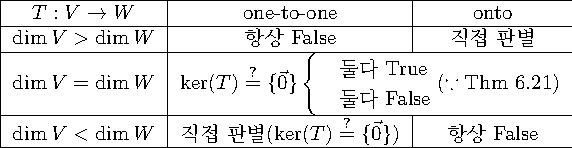
\includegraphics[scale = 1.0]{one-to-one+onto.pdf}
	\end{center}
\end{figure}

\section{The Matrix of a Linear Transformation + 3.6 Part II}

\textit{Definition.} Let $V$ and $W$ be vector spaces with $\dim V = n$ and $\dim W = m$. Let $\mathcal{B}$ and $\mathcal{C}$ be bases for $V$ and $W$, respectively, where $\mathcal{B} = \{ \textbf{v}_1, \cdots, \textbf{v}_n \}$. The \textbf{matrix of $T$ with respect to the bases $\mathcal{B}$ and $\mathcal{C}$}, denoted by $[T]_{ \mathcal{C} \leftarrow \mathcal{B} }$, is the $m \times n$ matrix defined by \begin{equation*}
	[T]_{ \mathcal{C} \leftarrow \mathcal{B} } = \begin{bmatrix}
	\left[ T(\textbf{v}_1) \right]_\mathcal{C} & \cdots & \left[ T(\textbf{v}_n) \right]_\mathcal{C}
	\end{bmatrix}
\end{equation*}
If $V = W$ and $\mathcal{B} = \mathcal{C}$, we write $[T]_{ \mathcal{B} \leftarrow \mathcal{B} }$ as $[T]_\mathcal{B}$ for short.

\begin{theorem}
	Let $V$ and $W$ be two finite-dimensional vector spaces with bases $\mathcal{B}$ and $\mathcal{C}$, respectively. If $T: V \rightarrow W$ is a linear transformation, \begin{equation*}
		[T]_{\mathcal{C} \leftarrow \mathcal{B}}[\textbf{v}]_\mathcal{B} = [T(\textbf{v})]_\mathcal{C}
	\end{equation*} for every vector $\textbf{v}$ in $V$. {\color{blue}Moreover, $[T]_{ \mathcal{C} \leftarrow \mathcal{B} }$ is the unique matrix with such property.}
\end{theorem}

\textbf{Theorem 3.30 \& Theorem 3.31} \\
The transformation $T: \mathbb{R}^n \rightarrow \mathbb{R}^m$ is a linear transformation if and only if $T$ is a matrix transformation: that is, $T$ is defined by \begin{equation*}
	T(\textbf{x}) = A\textbf{x}
\end{equation*} where $A$ is an $m \times n$ matrix.

\begin{proof}
	Let $\textbf{v}$ be a vector in $V$, then there exist scalars $c_1, \cdots, c_n$ such that \begin{equation*}
		\textbf{v} = c_1\textbf{v}_1 + \cdots + c_n\textbf{v}_n
	\end{equation*} since $\mathcal{B}$ is a basis for $V$. Thus, \begin{align*}
		[T(\textbf{v})]_\mathcal{C} &= [T(c_1\textbf{v}_1 + \cdots + c_n\textbf{v}_n)]_\mathcal{C} \\
		&= [c_1T(\textbf{v}_1) + \cdots + c_nT(\textbf{v}_n)]_\mathcal{C} \\
		&= c_1[T(\textbf{v}_1)]_\mathcal{C} + \cdots + c_n[T(\textbf{v}_n)]_\mathcal{C} \\
		&= \begin{bmatrix}
			\left[T(\textbf{v}_1)\right]_\mathcal{C} & \cdots & \left[T(\textbf{v}_n)\right]_\mathcal{C}
		\end{bmatrix}\begin{bmatrix}
			c_1 \\ \vdots \\ c_n
		\end{bmatrix} = [T]_\mathcal{ \mathcal{C} \leftarrow \mathcal{B} }[\textbf{v}]_\mathcal{B}
	\end{align*}
	\textbf{(Exercise 6.6 39)} Let $A$ be an $m \times n$ matrix such that \begin{equation*}
		A[\textbf{v}]_\mathcal{B} = [T(\textbf{v})]_\mathcal{C}
	\end{equation*} for all $\textbf{v} \in V$. For $i = 1, 2, \cdots, n$, \begin{equation*}
		A[\textbf{v}_i]_\mathcal{B} = A\textbf{e}_i = [T(\textbf{v}_i)]_\mathcal{C}
	\end{equation*} where $A\textbf{e}_i$ is the $i$th column of $A$. Therefore, $A$ is given as \begin{equation*}
		A = \begin{bmatrix}
			\left[T(\textbf{v}_1)\right]_\mathcal{C} & \cdots & [T(\textbf{v}_n)]_\mathcal{C}
		\end{bmatrix} = P_{ \mathcal{C} \leftarrow \mathcal{B} }
	\end{equation*} hence $P_{ \mathcal{C} \leftarrow \mathcal{B} }$ is the unique matrix with the given property.
\end{proof}

\begin{plaintheorem}
	Let $T: V \rightarrow W$ be a linear transformation between finite-dimensional vector spaces $V$ and $W$. Let $\mathcal{B}$ and $\mathcal{C}$ be bases for $V$ and $W$, respectively.
	\begin{enumerate}
		\item nullity($T$) = nullity($[T]_{ \mathcal{C} \leftarrow \mathcal{B}}$)
		\item rank($T$) = rank($[T]_{ \mathcal{C} \leftarrow \mathcal{B} }$)
	\end{enumerate}
\end{plaintheorem}

\begin{proof}
	Let $T: V \rightarrow W$ be a linear transformation between finite-dimensional vector spaces $V$ and $W$. Let $\mathcal{B}$ and $\mathcal{C}$ be bases for $V$ and $W$, respectively.
	\begin{enumerate}
		\item \textbf{(Exercise 6.6 40)} \\
		\begin{table}[H]
			\begin{center}
				\begin{tabular}{c}
					$\textbf{v} \in V$ is in ker($T$). \\
					\\
					$\Updownarrow$ \\
					\\
					$[T(\textbf{v})]_\mathcal{C} = [\textbf{0}]_\mathcal{C} = \textbf{0} = [T]_{ \mathcal{C} \leftarrow \mathcal{B} }[\textbf{v}]_\mathcal{B}$ (Theorem 6.26) \\
					\\
					$\Updownarrow$ \\
					\\
					$[\textbf{v}]_\mathcal{B}$ is in null($[T]_{ \mathcal{C} \leftarrow \mathcal{B} }$).
				\end{tabular}
			\end{center}
		\end{table}
		Since the coordinate vectors of distinct vectors in $V$ are distinct, nullity($T$) = dim(ker($T$)) = dim(null($[T]_{ \mathcal{C} \leftarrow \mathcal{B}} $)) = nullity($[T]_{ \mathcal{C} \leftarrow \mathcal{B}}$).
		\item \textbf{(Exercise 6.6 41)} Let $n = \dim V$. By the Rank Theorem for matrices and linear transformations, \begin{equation*}
			\textnormal{rank}(T) = n - \textnormal{nullity}(T) = n - \textnormal{nullity}([T]_{ \mathcal{C} \leftarrow \mathcal{B} }) = \textnormal{rank}([T]_{ \mathcal{C} \leftarrow \mathcal{B}} )
		\end{equation*}
	\end{enumerate}
\end{proof}

\begin{theorem}
	Let $U$, $V$, and $W$ be finite-dimensional vector spaces with bases $\mathcal{B}$, $\mathcal{C}$, and $\mathcal{D}$, respectively. Let $T: U \rightarrow V$ and $S: V \rightarrow W$ be linear transformations. Then \begin{equation*}
		[S \circ T]_{\mathcal{D} \leftarrow \mathcal{B} } = [S]_{ \mathcal{D} \leftarrow \mathcal{C} }[T]_{ \mathcal{C} \leftarrow \mathcal{B} }
	\end{equation*}
\end{theorem}

\textbf{Theorem 3.32 : Part 2} \\

 Let $T: \mathbb{R}^m \rightarrow \mathbb{R}^n$ and $S: \mathbb{R}^n \rightarrow \mathbb{R}^p$ be linear transformations. Then \begin{equation*}
	[S \circ T] = [S][T]
\end{equation*}

\begin{proof}
	Let $\mathcal{B} = \{\textbf{v}_1, \cdots, \textbf{v}_n\}$, then the $i$th column of $[S \circ T]_{ \mathcal{D} \leftarrow \mathcal{B} }$ is $[(S \circ T)(\textbf{v}_i)]_\mathcal{D}$, which is given as \begin{align*}
		[(S \circ T)(\textbf{v}_i)]_\mathcal{D} &= [S(T(\textbf{v}_i))]_\mathcal{D} \\
		&= [S]_{\mathcal{D} \leftarrow \mathcal{C}}[T(\textbf{v}_i)]_\mathcal{C} \\
		&= [S]_{\mathcal{D} \leftarrow \mathcal{C}}[T]_{\mathcal{C} \leftarrow \mathcal{B}}[\textbf{v}_i]_\mathcal{B} = [S]_{\mathcal{D} \leftarrow \mathcal{C}}[T]_{\mathcal{C} \leftarrow \mathcal{B}}\textbf{e}_i
	\end{align*} which is the $i$th column of $[S]_{\mathcal{D} \leftarrow \mathcal{C}}[T]_{\mathcal{C} \leftarrow \mathcal{B}}$. Therefore, $[S]_{\mathcal{D} \leftarrow \mathcal{C}}[T]_{\mathcal{C} \leftarrow \mathcal{B}} = [S \circ T]_{\mathcal{D} \leftarrow \mathcal{B}}$.
\end{proof}

\begin{theorem}
	Let $T: V \rightarrow W$ be a linear transformation between $n$-dimensional vector spaces $V$ and $W$, and let $\mathcal{B}$ and $\mathcal{C}$ be bases for $V$ and $W$, respectively. Then $T$ is invertible if and only if the matrix $[T]_{ \mathcal{C} \leftarrow \mathcal{B} }$ is invertible. Also, \begin{equation*}
		\inv{([T]_{ \mathcal{C} \leftarrow \mathcal{B} })} = [\inv{T}]_{ \mathcal{B} \leftarrow \mathcal{C} }
	\end{equation*}
\end{theorem}

\begin{proof}
	($\Rightarrow$) If $T$ is invertible, then there exists a linear transformation $\inv{T}$ such that $\inv{T} \circ T = I_V$. Then \begin{equation*}
		I = [I_V]_{ \mathcal{B} \leftarrow \mathcal{B} } = [\inv{T} \circ T]_{ \mathcal{B} \leftarrow \mathcal{B} } = [\inv{T}]_{ \mathcal{B} \leftarrow \mathcal{C} }[T]_{ \mathcal{C} \leftarrow \mathcal{B} }
	\end{equation*} Thus $\inv{([T]_{ \mathcal{C} \leftarrow \mathcal{B} })} = [\inv{T}]_{ \mathcal{B} \leftarrow \mathcal{C} }$. \\
	
	($\Leftarrow$) Suppose that $[T]_{ \mathcal{C} \leftarrow \mathcal{B} }$ is invertible. Let $\textbf{v}$ be a vector in ker($T$), then \begin{equation*}
		[T]_{ \mathcal{C} \leftarrow \mathcal{B} }[\textbf{v}]_\mathcal{B} = [T(\textbf{v})]_\mathcal{C} = [\textbf{0}]_\mathcal{C} = \textbf{0}
	\end{equation*} Thus, $[\textbf{v}]_\mathcal{B} = \textbf{0}$ by F.T.I.M, $\textbf{v} = \textbf{0}$ and  ker($T$) = $\{\textbf{0}\}$. Therefore, $T$ is one-to-one (Theorem 6.20) and since $\dim V = \dim W = n$, $T$ is onto (Theorem 6.21), hence $T$ is invertible (Theorem 6.24).
\end{proof}

\begin{theorem}
	Let $V$ be a finite-dimensional vector space with bases $\mathcal{B}$ and $\mathcal{C}$ and let $T: V \rightarrow V$ be a linear transformation. Then \begin{equation*}
		[T]_{ \mathcal{C} } = \inv{(P_{ \mathcal{B} \leftarrow \mathcal{C}})} [T]_{ \mathcal{B} } P_{ \mathcal{B} \leftarrow \mathcal{C} } = P_{ \mathcal{C} \leftarrow \mathcal{B} } [T]_{ \mathcal{B}  } P_{ \mathcal{B} \leftarrow \mathcal{C} }
	\end{equation*}
\end{theorem}

\textbf{Theorem 3.33} \\
The linear transformation $T: \mathbb{R}^n \rightarrow \mathbb{R}^n$ is invertible if and only if $[T]$ is an invertible matrix. If $T$ is invertible linear transformation, then \begin{equation*}
	[\inv{T}] = \inv{[T]}
\end{equation*}

\begin{proof}
	Note that $P_{ \mathcal{C} \leftarrow \mathcal{B} }$ is the matrix of $I_V$ with respect to the bases $\mathcal{B}$ and $\mathcal{C}$, since if $\mathcal{B} = \{\textbf{u}_1, \cdots, \textbf{u}_n\}$, \begin{equation*}
		P_{ \mathcal{C} \leftarrow \mathcal{B} } = \begin{bmatrix}
			\left[\textbf{u}_1\right]_\mathcal{C} & \cdots & \left[\textbf{u}_n\right]_\mathcal{C}
		\end{bmatrix} = \begin{bmatrix}
			\left[I_V(\textbf{u}_1)\right]_\mathcal{C} & \cdots & \left[I_V(\textbf{u}_n)\right]_\mathcal{C}
		\end{bmatrix} = [I_V]_{\mathcal{C} \leftarrow \mathcal{B}}
	\end{equation*} Similarly, $P_{ \mathcal{B} \leftarrow \mathcal{C} }$ is the matrix of $I_V$ with respect to the bases $\mathcal{C}$ and $\mathcal{B}$. Therefore, by Theorem 6.27, \begin{align*}
		[T]_{ \mathcal{C} \leftarrow \mathcal{C} } &= [I_V \circ T \circ I_V]_{ \mathcal{C} \leftarrow \mathcal{C} } \\
		&= [I_V]_{\mathcal{C} \leftarrow \mathcal{B}} [T]_{\mathcal{B} \leftarrow \mathcal{B}} [I_V]_{ \mathcal{B} \leftarrow \mathcal{C}} = P_{ \mathcal{C} \leftarrow \mathcal{B} }[T]_{ \mathcal{B} \leftarrow \mathcal{B} }P_{ \mathcal{B} \leftarrow \mathcal{C} }
	\end{align*}
\end{proof}

\textit{Note.} 교과서의 Theorem 3.33을 동치인 명제로 확장하였다. 그리고 $P_{ \mathcal{C} \leftarrow \mathcal{B} }$를 identity transformation의 행렬로 나타내는 것은 유용하니 알아 두자. \\
 
\textit{Definition.} Let $V$ be a finite-dimensional vector space and let $T: V \rightarrow V$ be a linear transformation. Then $T$ is called \textbf{diagonalizable} if there is a basis $\mathcal{C}$ for $V$ such that $[T]_\mathcal{C}$ is a diagonal matrix.

\begin{theorem} [The Fundamental Theorem of Invertible Matrices: Version 4]
	Let $A$ be an $n \times n$ matrix, and let $T: V \rightarrow W$ be a linear transformation such that its matrix $[T]_{ \mathcal{C} \leftarrow \mathcal{B} }$ with respect to the bases $\mathcal{B}$ and $\mathcal{C}$ of $V$ and $W$, respectively, is equal to $A$. The following propositions are equivalent:
	\begin{enumerate}
		\item $A$ is invertible.
		\item $A\textbf{x} = \textbf{b}$ has a unique solution for every $\textbf{b} \in$ \Rn.
		\item $A\textbf{x} = \textbf{0}$ has only the trivial solution.
		\item The RREF of $A$ is $I_n$.
		\item $A$ is a product of elementary matrices.
		\item rank($A$) = $n$
		\item nullity($A$) = $0$
		\item The columns of $A$ are linearly independent.
		\item The columns of $A$ span \Rn.
		\item The columns of $A$ form a basis for \Rn.
		\item The rows of $A$ are linearly independent.
		\item The rows of $A$ span \Rn.
		\item The rows of $A$ form a basis for \Rn.
		\item $ \det A \neq 0 $
		\item 0 is not an eigenvalue of $ A $.
		\item $T$ is invertible.
		\item $T$ is one-to-one.
		\item $T$ is onto.
		\item $\ker{T} = \{ \textbf{0} \}$
		\item range($T$) = $W$
	\end{enumerate}
\end{theorem}

\begin{proof}
	Since $A$ is $n \times n$ matrix, $\dim V = \dim W = n$, so Theorem 6.21 gives (q) $\Leftrightarrow$ (r). Theorem 6.24 gives (q) and (r) $\Leftrightarrow$ (p), and Theorem 6.20 gives (q) $\Leftrightarrow$ (s). (r) $\Leftrightarrow$ (t) holds since it is the definition of onto. Finally, Theorem 6.28 gives (a) $\Leftrightarrow$ (p).
\end{proof}
\iffalse
\section{Solutions for Exercises from Chapter 6}
\textbf{(6.1 1 to 11)} \\
True : \textbf{7} \\
Let $x, y, z \in \mathbb{R}^+$ and $c, d$ be scalars.
\begin{enumerate}
	\item (Axiom 1) \begin{equation*}
		x \oplus y = xy \in \mathbb{R}^+
	\end{equation*}
	\item (Axiom 2)\begin{equation*}
		x \oplus y = xy = yx = y \oplus x
	\end{equation*}
	\item (Axiom 3)\begin{equation*}
		(x \oplus y) \oplus z = xy \oplus z = xyz = x \oplus yz = x \oplus (y \oplus z)
	\end{equation*}
	\item (Axiom 4)\begin{equation*}
		\forall x \in \mathbb{R}^+, x \oplus 1 = x
	\end{equation*}
	which implies that $\textbf{0} = 1$.
	\item (Axiom 5)\begin{equation*}
		\forall x \in \mathbb{R}^+, x \oplus \frac{1}{x} = 1 = \textbf{0}
	\end{equation*}
	which implies that $-x = \frac{1}{x}$.
	\item (Axiom 6)\begin{equation*}
		c \odot x = x ^ c \in \mathbb{R}^+
	\end{equation*}
	\item (Axiom 7)\begin{equation*}
		c \odot (x \oplus y) = c \odot xy = (xy) ^ c = x^cy^c = x^c \oplus y^c = (c \odot x) \oplus (c \odot y)
	\end{equation*}
	\item (Axiom 8)\begin{equation*}
		(c + d) \odot x = x ^ {c + d} = x^cx^d = x^c \oplus x^d = (c \odot x) \oplus (d \odot x)
	\end{equation*}
	\item (Axiom 9)\begin{equation*}
		c \odot (d \odot x) = c \odot x^d = (x^d)^c = x^{cd} = (cd) \odot x
	\end{equation*}
	\item (Axiom 10)\begin{equation*}
		1 \odot x = x ^ 1 = x
	\end{equation*}
\end{enumerate}
Therefore, the given set is a vector space. \\

False : \textbf{6} \\
Let $\textbf{u} = \textbf{v} = \begin{bmatrix}
	1 \\ 1
\end{bmatrix} \in \mathbb{R}^2$. Then \begin{equation*}
	2(\textbf{u} \oplus \textbf{v}) = 2(\begin{bmatrix}
	 1 \\ 1
	\end{bmatrix} \oplus \begin{bmatrix}
	 1 \\ 1
	\end{bmatrix}) = 2\begin{bmatrix}
	 3 \\ 3
	\end{bmatrix} = \begin{bmatrix}
	 6 \\ 6
	\end{bmatrix} \neq \begin{bmatrix}
	 5 \\ 5
	\end{bmatrix} = \begin{bmatrix}
	 2 \\ 2
	\end{bmatrix} \oplus \begin{bmatrix}
	 2 \\ 2
	\end{bmatrix} = 2\begin{bmatrix}
	 1 \\ 1
	\end{bmatrix} \oplus 2\begin{bmatrix}
	 1 \\ 1
	\end{bmatrix} = 2\textbf{u} \oplus 2\textbf{v}
\end{equation*}
Therefore Axiom 7 fails to hold, hence the given set is not a vector space. \\

\textbf{(6.1 24 to 45)} \\
True : \textbf{26} \\
Since $\begin{bmatrix}
	0 \\ 0 \\ 0
\end{bmatrix} \in W$, $W$ is a nonempty subset of $V$. Let $\textbf{u} = \begin{bmatrix}
	u \\ 0 \\ u
\end{bmatrix}, \textbf{v} = \begin{bmatrix}
	v \\ 0 \\ v
\end{bmatrix}$ be vectors in $W$ where $u, v \in \mathbb{R}$, and $c$ a scalar. Then \begin{align*}
	\textbf{u} + \textbf{v} &= \begin{bmatrix}
	u \\ 0 \\ u
	\end{bmatrix} + \begin{bmatrix}
	v \\ 0 \\ v
	\end{bmatrix} = \begin{bmatrix}
	u + v \\ 0 \\ u + v
	\end{bmatrix} \in W \\
	c\textbf{u} &= c\begin{bmatrix}
	u \\ 0 \\ u
	\end{bmatrix} = \begin{bmatrix}
	cu \\ 0 \\ cu
	\end{bmatrix} \in W
\end{align*}
Therefore, by Theorem 6.2, $W$ is a subspace of $V$. \\

False : \textbf{27} \\
Let $\textbf{w} = \begin{bmatrix}
	-1 \\ 0 \\ 1
\end{bmatrix} \in W$. However, \begin{equation*}
	(-1)\textbf{w} = \begin{bmatrix}
		1 \\ 0 \\ -1
	\end{bmatrix} \notin W
\end{equation*} so $W$ is not a subspace of $V$. \\

\textbf{(6.1 46)} \\
Since $U$ and $W$ are subspaces of $V$, $\textbf{0} \in U$ and $\textbf{0} \in W$, so $\textbf{0} \in U \cap W$. Thus, $U \cap W$ is a nonempty subset of $V$. \\

Let $\textbf{v}_1, \textbf{v}_2$ be vectors in $U \cap W$ and $c$ be a scalar. Since $U, W$ are subspaces of $V$  and $\textbf{v}_1, \textbf{v}_2 \in U$ and $\textbf{v}_1, \textbf{v}_2 \in W$, \begin{align*}
	\textbf{v}_1 + \textbf{v}_2 \in U \mbox{ and } \textbf{v}_1 + \textbf{v}_2 \in W &\Rightarrow \textbf{v}_1 + \textbf{v}_2 \in U \cap W \\
	c\textbf{v}_1 \in U \mbox{ and } c\textbf{v}_1 \in W &\Rightarrow c\textbf{v}_1 \in U \cap W
\end{align*} Therefore, by Theorem 6.2, $U \cap W$ is a subspace of $V$. \\

\textbf{(6.1 47)} \\
Let $V = \mathbb{R}^2$ and let $U$ = span$\left(\begin{bmatrix}
	1 \\ 0
\end{bmatrix}\right)$, $W$ = span$\left(\begin{bmatrix}
	0 \\ 1
\end{bmatrix}\right)$ then $U$ and $W$ are subspaces of $V$. Then $\begin{bmatrix}
	1 \\ 0
\end{bmatrix}, \begin{bmatrix}
	0 \\ 1
\end{bmatrix} \in U \cup W$, but $\begin{bmatrix}
	1 \\ 0
\end{bmatrix} + \begin{bmatrix}
	0 \\ 1
\end{bmatrix} = \begin{bmatrix}
	1 \\ 1
\end{bmatrix} \notin U \cup W$. Therefore, $U \cup W$ is not a subspace of $V$. \\

\textbf{(6.1 63) : Uniqueness of the Identity Element} \\
Let $V$ be a vector space. Suppose that there are more than two zero vectors in $V$, and let $\textbf{0}$ and $\textbf{0}'$ be any two of them. By Axiom 2 and Axiom 4, \begin{equation*}
	\textbf{0} = \textbf{0} + \textbf{0}' = \textbf{0}' + \textbf{0} = \textbf{0}'
\end{equation*} Therefore, $V$ has a unique zero vector. \\

\textbf{(6.1 64) : Uniqueness of the Inverse Element} \\
Let $V$ be a vector space, and let $\textbf{0}$ be a zero vector of $V$. Suppose that for $\textbf{v} \in V$, there exist two vectors $\textbf{v}_1$ and $\textbf{v}_2$ such that $\textbf{v} + \textbf{v}_1 = \textbf{v} + \textbf{v}_2 = \textbf{0}$. Then \begin{align*}
	\textbf{v}_1 &= \textbf{v}_1 + \textbf{0} \mbox{ (Axiom 4) } \\
	&= \textbf{v}_1 + (\textbf{v} + \textbf{v}_2) \\
	&= (\textbf{v} + \textbf{v}_1) + \textbf{v}_2 \mbox{ (Axiom 2 and Axiom 3) } \\
	&= \textbf{0} + \textbf{v}_2 = \textbf{v}_2 \mbox{ (Axiom 4) }
\end{align*}
Therefore, there is a unique $\textbf{v}'$ such that $\textbf{v} + \textbf{v}' = \textbf{0}$. \\

\textbf{(6.2 15)} \\
Suppose that $f$ and $g$ are linearly dependent, then one of $f$ and $g$ is a scalar multiple of the other, by Theorem 6.4. Without loss of generality, we may assume that \begin{equation*}
	^\forall x, f(x) = cg(x) \mbox{ for some } c \in \mathbb{R}
\end{equation*} Then \begin{equation*}
	^\forall x, f'(x) = cg'(x)
\end{equation*} So the Wronskian of $f$ and $g$ are given by \begin{equation*}
	W(x) = \begin{vmatrix}
		f(x) & g(x) \\ f'(x) & g'(x)
	\end{vmatrix} = f(x)g'(x) - g(x)f'(x) = cg(x)g'(x) - cg(x)g'(x) = 0
\end{equation*} Therefore, the contraposition - if $^\exists x$ such that $W(x) \neq 0$, then $f$ and $g$ are linearly independent - is also true. \\

\textbf{(6.2 17)} \\
(a) Suppose that $\textbf{u} + \textbf{v}, \textbf{v} + \textbf{w}, \textbf{w} + \textbf{u}$ are linearly dependent, then there exist scalars $c_1, c_2, c_3$, at least one of which is nonzero, such that \begin{equation*}
	c_1(\textbf{u} + \textbf{v}) + c_2(\textbf{v} + \textbf{w}) + c_2(\textbf{w} + \textbf{u}) = \textbf{0}
\end{equation*} Then \begin{equation*}
	(c_1 + c_3)\textbf{u} + (c_1 + c_2)\textbf{v} + (c_2 + c_3)\textbf{w} = \textbf{0}
\end{equation*} Since $\textbf{u}, \textbf{v}, \textbf{w}$ are linearly independent, $c_1 + c_3 = c_1 + c_2 = c_2 + c_3 = 0$. This implies that $c_1 = c_2 = c_3 = 0$, which is a contradiction. Therefore, $\{\textbf{u} + \textbf{v}, \textbf{v} + \textbf{w}, \textbf{w} + \textbf{u}\}$ is linearly independent. \\

(b) The given set $\{\textbf{u} - \textbf{v}, \textbf{v} - \textbf{w}, \textbf{u} - \textbf{w}\}$ is linearly dependent since \begin{equation*}
	(\textbf{u} - \textbf{v}) + (\textbf{v} - \textbf{w}) - (\textbf{u} - \textbf{w}) = \textbf{0}
\end{equation*}

\textbf{(6.1 48 + 6.2 42) : Subspace $U + W$} \\
Let $V$ be a vector space, and let $U, W$ be subspaces of $V$. Then the \textbf{sum of $U$ and $W$}, denoted by $U + W$, is defined by \begin{equation*}
	U + W = \{\textbf{u} + \textbf{w} \vert \textbf{u} \in U \mbox{ and } \textbf{w} \in W\}
\end{equation*}

\textbf{6.1 48a} \\
(i) Let $\begin{bmatrix}
	x \\ y \\ 0
\end{bmatrix}$ be a vector in $\left\lbrace\left.\begin{bmatrix}
	t_1 \\ t_2 \\ 0
\end{bmatrix} \right\vert t_1, t_2 \in \mathbb{R} \right\rbrace$. Since $
	\begin{bmatrix}
		x \\ y \\ 0
	\end{bmatrix} = \begin{bmatrix}
		x \\ 0 \\ 0
	\end{bmatrix} + \begin{bmatrix}
		0 \\ y \\ 0
	\end{bmatrix}$ and $\begin{bmatrix}
	x \\ 0 \\ 0
\end{bmatrix} \in U$, $\begin{bmatrix}
	0 \\ y \\ 0
\end{bmatrix} \in W$, $\begin{bmatrix}
	x \\ y \\ 0
\end{bmatrix} \in U + W$. \\

(ii) Let $\textbf{x} \in U + W$, then there exist $\textbf{u} = \begin{bmatrix}
	u \\ 0 \\ 0
\end{bmatrix} \in U$ and $\textbf{w} = \begin{bmatrix}
	0 \\ w \\ 0
\end{bmatrix} \in W$ such that $\textbf{x} = \textbf{u} + \textbf{w}$, where $u, w \in \mathbb{R}$. Then $\textbf{x} = \begin{bmatrix}
	u \\ 0 \\ 0
\end{bmatrix} + \begin{bmatrix}
	0 \\ w \\ 0
\end{bmatrix} = \begin{bmatrix}
	u \\ w \\ 0
\end{bmatrix} \in \left\lbrace\left.\begin{bmatrix}
	t_1 \\ t_2 \\ 0
\end{bmatrix} \right\vert t_1, t_2 \in \mathbb{R} \right\rbrace$. \\

By (i) and (ii), $U + W = \left\lbrace\left.\begin{bmatrix}
	t_1 \\ t_2 \\ 0
\end{bmatrix} \right\vert t_1, t_2 \in \mathbb{R} \right\rbrace$.

\textbf{6.1 48b} \\
Since $\textbf{0} \in U$ and $\textbf{0} \in  W$, $\textbf{0} = \textbf{0} + \textbf{0} \in U + W$ so $U + W$ is a nonempty subset of $V$. \\

Let $\textbf{x}_1, \textbf{x}_2$ be vectors in $U + W$, then there exist vectors $\textbf{u}_1, \textbf{u}_2 \in U$ and $\textbf{w}_1, \textbf{w}_2 \in W$ such that $\textbf{x}_1 = \textbf{u}_1 + \textbf{w}_1$ and $\textbf{x}_2 = \textbf{u}_2 + \textbf{w}_2$. Let $c$ be a scalar, then \begin{align*}
	\textbf{x}_1 + \textbf{x}_2 &= (\textbf{u}_1 + \textbf{w}_1) + (\textbf{u}_2 + \textbf{w}_2) = (\textbf{u}_1 + \textbf{u}_2) + (\textbf{w}_1 + \textbf{w}_2) \\
	c\textbf{x}_1 &= c(\textbf{u}_1 + \textbf{w}_1) = c\textbf{u}_1 + c\textbf{w}_1
\end{align*} Since $U$ and $W$ are subspaces of $V$, $\textbf{u}_1 + \textbf{u}_2, c\textbf{u}_1 \in U$ and $\textbf{w}_1 + \textbf{w}_2, c\textbf{w}_1 \in W$. Therefore, $\textbf{x}_1 + \textbf{x}_2 \in U + W$ and $c\textbf{x}_1 \in U + W$, hence $U + W$ is a subspace of $V$. \\

\textbf{6.2 42} \\
Since $U \cap W$ is a vector space (Exercise 6.1 46), let $\mathcal{B} = \{\textbf{v}_1, \cdots, \textbf{v}_k\}$ be a basis for $U \cap W$. Since $\mathcal{B}$ is a linearly independent set in $U$ and $W$, by Theorem 6.10(e), let $\mathcal{C} = \{\textbf{v}_1, \cdots, \textbf{v}_k, \textbf{u}_1, \cdots, \textbf{u}_m\}$ be a basis for $U$ extended from $\mathcal{B}$, and let $\mathcal{D} = \{\textbf{v}_1, \cdots, \textbf{v}_k, \textbf{w}_1, \cdots, \textbf{w}_n\}$ be a basis for $W$ extended from $\mathcal{B}$. \\

Let $\textbf{x}$ be a vector in $U + W$, then there exist vectors $\textbf{u} \in U$ and $\textbf{w} \in W$ such that $\textbf{x} = \textbf{u} + \textbf{w}$. Then $\textbf{u}$ is expressed as a linear combination of the vectors in $\mathcal{C}$ and $\textbf{w}$ is expressed as a linear combination of the vectors in $\mathcal{D}$. Thus, $\textbf{x}$ is a linear combination of the vectors in $\mathcal{C} \cup \mathcal{D} = \{\textbf{v}_1, \cdots, \textbf{v}_k, \textbf{u}_1, \cdots, \textbf{u}_m, \textbf{w}_1, \cdots, \textbf{w}_n\}$. This implies that $\mathcal{C} \cup \mathcal{D}$ spans $U + W$. \\

Now, suppose that $\mathcal{C} \cup \mathcal{D}$ is linearly dependent. Then there exist scalars $c_1, \cdots, c_k, d_1, \cdots, d_m, e_1, \cdots, e_n$, at least one of which is nonzero, such that \begin{equation*}
	c_1\textbf{v}_1 + \cdots + c_k\textbf{v}_k + d_1\textbf{u}_1 + \cdots + d_m\textbf{u}_m + e_1\textbf{w}_1 + \cdots + e_n\textbf{w}_n = \textbf{0}
\end{equation*} Let $\textbf{v} = c_1\textbf{v}_1 + \cdots + c_k\textbf{v}_k, \textbf{u} = d_1\textbf{u}_1 + \cdots + d_m\textbf{u}_m, \textbf{w} = e_1\textbf{w}_1 + \cdots + e_n\textbf{w}_n$, then $\textbf{v} + \textbf{u} + \textbf{w} = \textbf{0}$. If $\textbf{u} = \textbf{0}$, then $\textbf{v} + \textbf{w} = \textbf{0}$, which is a contradiction since $\mathcal{D}$ is a linearly independent set in $V$. Thus, $\textbf{u} \neq \textbf{0}$, and by similar procedure, $\textbf{w} \neq \textbf{0}$. \\

Since $\textbf{w} = -\textbf{u} - \textbf{v}$, $\textbf{w}$ is in both  span($\mathcal{D}$) = $W$ and span($\mathcal{C}$) = $U$, so $\textbf{w}$ is in $U \cap W$. However, $\textbf{w}$ is not a linear combination of vectors in $\mathcal{B}$, since it is already a linear combination of $\textbf{w}_1, \cdots, \textbf{w}_n$. Therefore, $\mathcal{C} \cup \mathcal{D}$ should be linearly independent. \\

Therefore, $\mathcal{C} \cup \mathcal{D}$ is a basis for $U + W$. So \begin{equation*}
	\dim(U + W) = k + m + n = (k + m) + (k + n) - k = \dim U + \dim W - \dim(U \cap V)
\end{equation*}

\textbf{(6.1 49 + 6.1 50 + 6.2 43) : Vector Space $U \times W$} \\
문제의 조건이 불완전하다. $U \times W$가 vector space임을 보이기 위해서는 상위의 vector space가 주어졌거나, vector addition과 scalar multiplication이 정의되어야 하는데 둘 다 없으므로 원래 증명을 할 수 없네요 ㅠㅠ \\

If $U$ and $V$ are vector spaces, the \textbf{Cartesian Product} of $U$ and $V$, denoted by $U \times V$, is defined by \begin{equation*}
	U \times V = \{ (\textbf{u}, \textbf{v}) \mid \textbf{u} \in U \mbox{ and } \textbf{v} \in V \}
\end{equation*}
The addition between two vectors $(\textbf{u}_1, \textbf{v}_1)$ and $(\textbf{u}_2, \textbf{v}_2)$ in $U \times V$ is defined by \begin{equation*}
	(\textbf{u}_1, \textbf{v}_1) + (\textbf{u}_2, \textbf{v}_2) = (\textbf{u}_1 + \textbf{u}_2, \textbf{v}_1 + \textbf{v}_2)
\end{equation*}
The scalar multiplication between a vector $(\textbf{u}, \textbf{v})$ in $U \times V$ and a scalar $c$ is defined by \begin{equation*}
	c(\textbf{u}, \textbf{v}) = (c\textbf{u}, c\textbf{v})
\end{equation*}

\textbf{6.1 49} \\
Let $(\textbf{u}_1, \textbf{v}_1), (\textbf{u}_2, \textbf{v}_2), (\textbf{u}_3, \textbf{v}_3)$ be vectors of $U \times V$ and let $c, d$ be scalars.
\begin{enumerate}
	\item (Axiom 1) Since $U$ and $V$ are vector spaces, $\textbf{u}_1 + \textbf{u}_2 \in U$ and $\textbf{v}_1 + \textbf{v}_2 \in V$. So \begin{equation*}
		(\textbf{u}_1, \textbf{v}_1) + (\textbf{u}_2 , \textbf{v}_2) = (\textbf{u}_1 + \textbf{u}_2, \textbf{v}_1 + \textbf{v}_2) \in U \times V
	\end{equation*} 
	\item (Axiom 2) \begin{equation*}
		(\textbf{u}_1, \textbf{v}_1) + (\textbf{u}_2, \textbf{v}_2) = (\textbf{u}_1 + \textbf{u}_2, \textbf{v}_1 + \textbf{v}_2) = (\textbf{u}_2 + \textbf{u}_1 , \textbf{v}_2 + \textbf{v}_1) = (\textbf{u}_2, \textbf{v}_2) + (\textbf{u}_1, \textbf{v}_1)
	\end{equation*}
	\item (Axiom 3) \begin{align*}
	((\textbf{u}_1, \textbf{v}_1) + (\textbf{u}_2, \textbf{v}_2)) + (\textbf{u}_3, \textbf{v}_3) &= (\textbf{u}_1 + \textbf{u}_2, \textbf{v}_1 + \textbf{v}_2) + (\textbf{u}_3, \textbf{v}_3) \\
	&= (\textbf{u}_1 + \textbf{u}_2 + \textbf{u}_3, \textbf{v}_1 + \textbf{v}_2 + \textbf{v}_3) \\
	&= (\textbf{u}_1, \textbf{v}_1) + (\textbf{u}_2 + \textbf{u}_3, \textbf{v}_2 + \textbf{v}_3) \\
	&= (\textbf{u}_1 ,\textbf{v}_1) + ((\textbf{u}_2, \textbf{v}_2) + (\textbf{u}_3, \textbf{v}_3))
	\end{align*}
	\item (Axiom 4) For any vector $(\textbf{u}, \textbf{v}) \in U \times V$, \begin{equation*}
		(\textbf{u}, \textbf{v}) + (\textbf{0}, \textbf{0}) = (\textbf{u} + \textbf{0}, \textbf{v} + \textbf{0}) = (\textbf{u} + \textbf{v})
	\end{equation*} So the zero vector of $U \times V$ is given by $\textbf{0} = (\textbf{0}, \textbf{0})$.
	\item (Axiom 5) For any vector $(\textbf{u}, \textbf{v}) \in U \times V$, \begin{equation*}
		(\textbf{u}, \textbf{v}) + (-\textbf{u}, -\textbf{v}) = (\textbf{u} - \textbf{u}, \textbf{v} - \textbf{v}) = (\textbf{0}, \textbf{0}) = \textbf{0}
	\end{equation*} So the inverse element of $(\textbf{u}, \textbf{v})$ is given by $-(\textbf{u}, \textbf{v}) = (-\textbf{u}, -\textbf{v})$.
	\item (Axiom 6) Since $U$ and $V$ are vector spaces, $c\textbf{u}_1 \in U$ and $c\textbf{v}_1 \in V$. So \begin{equation*}
		c(\textbf{u}_1, \textbf{v}_1) = (c\textbf{u}_1, c\textbf{v}_1) \in U \times V
	\end{equation*}
	\item (Axiom 7) \begin{align*}
		c((\textbf{u}_1, \textbf{v}_1) + (\textbf{u}_2, \textbf{v}_2)) &= c(\textbf{u}_1 + \textbf{u}_2, \textbf{v}_1 + \textbf{v}_2) \\
		&= (c\textbf{u}_1 + c\textbf{u}_2, c\textbf{v}_1 + c\textbf{v}_2) \\
		&= (c\textbf{u}_1, c\textbf{v}_1) + (c\textbf{u}_2, c\textbf{v}_2) = c(\textbf{u}_1, \textbf{v}_1) + c(\textbf{u}_2, \textbf{v}_2)
	\end{align*}
	\item (Axiom 8) \begin{align*}
		(c + d)(\textbf{u}_1, \textbf{v}_1) &= ((c+d)\textbf{u}_1, (c+d)\textbf{v}_1) \\
		&= (c\textbf{u}_1 + d\textbf{u}_1, c\textbf{v}_1 + d\textbf{v}_1) = (c\textbf{u}_1, c\textbf{v}_1) + (d\textbf{u}_1, d\textbf{v}_1) = c(\textbf{u}_1, \textbf{v}_1) + d(\textbf{u}_1, \textbf{v}_1)
	\end{align*}
	\item (Axiom 9) \begin{align*}
		c(d(\textbf{u}, \textbf{v})) = c(d\textbf{u}, d\textbf{v}) = (cd\textbf{u}, cd\textbf{v}) = (cd)(\textbf{u}, \textbf{v})
	\end{align*}
	\item (Axiom 10) \begin{align*}
		1(\textbf{u}, \textbf{v}) = (1\textbf{u}, 1\textbf{v}) = (\textbf{u}, \textbf{v})
	\end{align*}
\end{enumerate}
Therefore, $U \times V$ is a vector space. \\

\textbf{6.1 50} \\
Since $\textbf{0} \in W$, $(\textbf{0}, \textbf{0}) \in \Delta$ so $\Delta$ is a nonempty subset of $V \times V$. \\

Let $(\textbf{w}_1, \textbf{w}_1), (\textbf{w}_2, \textbf{w}_2)$ be vectors in $\Delta$ and $c$ be a scalar. Since $W$ is a subspace of $V$, $\textbf{w}_1 + \textbf{w}_2 \in W$ and $c\textbf{w}_1 \in W$. Then \begin{align*}
	(\textbf{w}_1, \textbf{w}_1) + (\textbf{w}_2, \textbf{w}_2) &= (\textbf{w}_1 + \textbf{w}_2, \textbf{w}_1 + \textbf{w}_2) \in \Delta \\
	c(\textbf{w}_1, \textbf{w}_1) &= (c\textbf{w}_1, c\textbf{w}_1) \in \Delta
\end{align*} Therefore, $\Delta$ is a subspace of $V \times V$ by Theorem 6.2. \\

\textbf{6.2 43a} \\
Let $\mathcal{B} = \{\textbf{u}_1, \cdots, \textbf{u}_m\}$ be a basis for $U$ and let $\mathcal{C} = \{\textbf{v}_1, \cdots, \textbf{v}_n\}$ be a basis for $V$. Let $\mathcal{D} = \{(\textbf{u}_1, \textbf{0}), \cdots, (\textbf{u}_m, \textbf{0}), (\textbf{0}, \textbf{v}_1), \cdots, (\textbf{0}, \textbf{v}_n)\}$, then $\mathcal{D}$ is a subset of $U \times V$. \\

Let $(\textbf{u}, \textbf{v})$ be a vector in $U \times V$. Then there exist scalars $c_1, \cdots, c_m, d_1, \cdots, d_n$ such that \begin{equation*}
	\textbf{u} = c_1\textbf{u}_1 + \cdots + c_m\textbf{u}_m \mbox{ and } \textbf{v} = d_1\textbf{v}_1 + \cdots + d_n\textbf{v}_n
\end{equation*} Then \begin{align*}
	(\textbf{u}, \textbf{v}) &= (c_1\textbf{u}_1 + \cdots + c_m\textbf{u}_m, d_1\textbf{v}_1 + \cdots + d_n\textbf{v}_n) \\
	&= c_1(\textbf{u}_1, \textbf{0}) + \cdots + c_m(\textbf{u}_m, \textbf{0}) + d_1(\textbf{0}, \textbf{v}_1) + \cdots + d_n(\textbf{0}, \textbf{v}_n)
\end{align*} so $\textbf{u} \in$ span($\mathcal{D}$), hence $\mathcal{D}$ spans $U \times V$. \\

Consider the scalars $c_1, \cdots, c_m, d_1, \cdots, d_n$ such that \begin{equation*}
	c_1(\textbf{u}_1, \textbf{0}) + \cdots + c_m(\textbf{u}_m, \textbf{0}) + d_1(\textbf{0}, \textbf{v}_1) + \cdots + d_n(\textbf{0}, \textbf{v}_n) = \textbf{0} = (\textbf{0}, \textbf{0})
\end{equation*} Since \begin{align*}
	c_1(\textbf{u}_1, \textbf{0}) + \cdots + c_m(\textbf{u}_m, \textbf{0}) + d_1(\textbf{0}, \textbf{v}_1) + \cdots + d_n(\textbf{0}, \textbf{v}_n) = (c_1\textbf{u}_1 + \cdots + c_m\textbf{u}_m, d_1\textbf{v}_1 + \cdots + d_1\textbf{v}_n)
\end{align*} $c_1\textbf{u}_1 + \cdots + c_m\textbf{u}_m = \textbf{0}$ and $d_1\textbf{v}_1 + \cdots + d_1\textbf{v}_n = \textbf{0}$. Since $\mathcal{B}$ and $\mathcal{C}$ are linearly independent, this implies that $c_1 = \cdots = c_m = d_1 = \cdots = d_n = 0$. Thus, $\mathcal{D}$ is linearly independent. \\

Therefore, $\mathcal{D}$ is a basis for $U \times V$, hence $\dim(U \times V) = m + n = \dim U + \dim V$. \\

\textbf{6.2 43b} \\
Let $\mathcal{B} = \textbf{w}_1, \cdots, \textbf{w}_k$ be a basis for $W$, and let $\mathcal{C} = \{(\textbf{w}_1, \textbf{w}_1), \cdots, (\textbf{w}_k, \textbf{w}_k)\}$, then $\mathcal{C}$ is a subset for $\Delta$. \\

Let $(\textbf{w}, \textbf{w})$ be vector in $\Delta$, then since $\textbf{w} \in W$, there exist scalars $c_1, \cdots, c_k$ such that \begin{equation*}
	\textbf{w} = c_1\textbf{w}_1 + \cdots + c_k\textbf{w}_k
\end{equation*} Then \begin{equation*}
	(\textbf{w}, \textbf{w}) = (c_1\textbf{w}_1 + \cdots + c_k\textbf{w}_k, c_1\textbf{w}_1 + \cdots + c_k\textbf{w}_k) = c_1(\textbf{w}_1, \textbf{w}_1) + \cdots + c_k(\textbf{w}_k, \textbf{w}_k)
\end{equation*} so $(\textbf{w}, \textbf{w}) \in$ span($\mathcal{C}$), hence $\mathcal{C}$ spans $\Delta$. \\

Consider the scalars $c_1, \cdots, c_k$ such that \begin{equation*}
	c_1(\textbf{w}_1, \textbf{w}_1) + \cdots + c_k(\textbf{w}_k, \textbf{w}_k) = \textbf{0} = (\textbf{0}, \textbf{0})
\end{equation*} Then \begin{equation*}
	c_1(\textbf{w}_1, \textbf{w}_1) + \cdots + c_k(\textbf{w}_k, \textbf{w}_k) = (c_1\textbf{w}_1 + \cdots + c_k\textbf{w}_k, c_1\textbf{w}_1 + \cdots + c_k\textbf{w}_k)
\end{equation*} so $c_1\textbf{w}_1 + \cdots + c_k\textbf{w}_k = \textbf{0}$. Since $\mathcal{B}$ is linearly independent, this implies that $c_1 = \cdots = c_k = 0$. Thus, $\mathcal{C}$ is linearly independent. \\

Therefore, $\mathcal{C}$ is a basis for $\Delta$, hence $\dim \Delta = k = \dim W$. \\

\textbf{(6.2 44)} \\
Let $\mathcal{B}$ be a finite set of polynomials. Suppose that $\mathcal{B}$ is a basis for $\mathscr{P}$, and let $n$ be the highest degree of the polynomials in $\mathcal{B}$. Then $x^{n+1}$ cannot be represented as linear combination of polynomials in $\mathcal{B}$, so $\mathcal{B}$ cannot span $\mathscr{P}$, which is a contradiction. Therefore, $\mathscr{P}$ cannot have finite basis, hence $\mathscr{P}$ is infinite-dimensional. \\

\textbf{(6.2 57)} \\
Suppose that $c_1\textbf{v}_1, \cdots, c_n\textbf{v}_n$ are linearly dependent. Then there exist scalars $d_1, \cdots, d_n$, at least one of which is nonzero, such that \begin{align*}
	d_1(c_1\textbf{v}_1) + \cdots + d_n(c_n\textbf{v}_n) = c_1d_1\textbf{v}_1 + \cdots + c_nd_n\textbf{v}_n = \textbf{0}
\end{align*} Since $\textbf{v}_1, \cdots, \textbf{v}_n$ are linearly independent, this implies that $c_1d_1 = c_2d_2 = \cdots = c_nd_n = 0$. Since $c_1, \cdots, c_n$ are nonzero scalars, $d_1 = \cdots = d_n = 0$, which is a contradiction. Thus, $\{c_1\textbf{v}_1, \cdots, c_n\textbf{v}_n\}$ is linearly independent. Since $\dim V = n$ and $\{c_1\textbf{v}_1, \cdots, c_n\textbf{v}_n\}$ is a linearly independent set in $V$ with $n$ vectors, $\{c_1\textbf{v}_1, \cdots, c_n\textbf{v}_n\}$ is a basis for $V$ by Theorem 6.10(c). \\

\textbf{(6.2 58)} \\
Consider the scalars $c_1, \cdots, c_n$ such that \begin{equation*}
	c_1\textbf{v}_1 + c_2(\textbf{v}_1 + \textbf{v}_2) + \cdots + c_n(\textbf{v}_1 + \cdots + \textbf{v}_n) = \textbf{0}
\end{equation*} Then \begin{align*}
	&c_1\textbf{v}_1 + c_2(\textbf{v}_1 + \textbf{v}_2) + \cdots + c_n(\textbf{v}_1 + \cdots + \textbf{v}_n) \\
	&= (c_1 + \cdots + c_n)\textbf{v}_1 + (c_2 + \cdots + c_n)\textbf{v}_2 + \cdots + c_n\textbf{v}_n = \textbf{0}
\end{align*} Since $\textbf{v}_1, \cdots, \textbf{v}_n$ are linearly independent, this implies that \begin{equation*}
	c_1 + \cdots + c_n = c_2 + \cdots + c_n = \cdots = c_n = 0
\end{equation*} Thus $c_1 = c_2 = \cdots = c_n = 0$, hence $\{\textbf{v}_1, \textbf{v}_1 + \textbf{v}_2, \cdots, \textbf{v}_1 + \cdots + \textbf{v}_n\}$ is linearly independent. Since $\dim V = n$ and $\{\textbf{v}_1, \textbf{v}_1 + \textbf{v}_2, \cdots, \textbf{v}_1 + \cdots + \textbf{v}_n\}$ is a linearly independent set in $V$ with $n$ vectors, $\{\textbf{v}_1, \textbf{v}_1 + \textbf{v}_2, \cdots, \textbf{v}_1 + \cdots + \textbf{v}_n\}$ is a basis for $V$ by Theorem 6.10(c). \\

\textit{Note.} Theorem 6.10을 이용해서 주어진 집합이 일차독립 / spanning set 중 하나만 보여도 basis임을 증명할 수 있다. 57번에서는 귀류법을 사용해서 일차독립임을 보였고, 58번에서는 직접 증명했는데 서술 방식이 다르니 참고. \\

\textbf{(6.2 59 + 6.2 60 + 6.2 61 + 6.2 62) : Lagrange Polynomials} \\
Let $a_0, \cdots, a_n$ be distinct real numbers. The \textbf{Lagrange Polynomials} associated with $a_i$, denoted by $p_i(x)$, is defined by \begin{equation*}
	p_i(x) = \frac{(x - a_0) \cdots (x - a_{i-1})(x - a_{i+1}) \cdots (x - a_n)}{(a_i - a_0) \cdots (a_i - a_{i-1})(a_i - a_{i+1}) \cdots (a_i - a_n)}
\end{equation*}

\textbf{59a} \\
\begin{align*}
	p_0(x) &= \frac{(x - 2)(x - 3)}{(1 - 2)(1 - 3)} = \frac{1}{2}x^2 - \frac{5}{2}x + 3 \\
	p_1(x) &= \frac{(x - 1)(x - 3)}{(2 - 1)(2 - 3)} = -x^2 + 4x - 3 \\
	p_2(x) &= \frac{(x - 1)(x - 2)}{(3 - 1)(3 - 2)} = \frac{1}{2}x^2 - \frac{3}{2}x + 1
\end{align*}

\textbf{59b} \\
If $i \neq j$, $(x - a_j)$ is a factor of $p_i(x)$, so $p_i(a_j) = 0$. If $i = j$, \begin{equation*}
	p_i(a_i) = \frac{(a_i - a_0) \cdots (a_i - a_{i-1})(a_i - a_{i+1}) \cdots (a_i - a_n)}{(a_i - a_0) \cdots (a_i - a_{i-1})(a_i - a_{i+1}) \cdots (a_i - a_n)} = 1
\end{equation*}

\textbf{60a} \\
Let $\mathcal{B} = \{p_0(x), \cdots, p_n(x)\}$. Consider the scalars $c_0, \cdots, c_n$ such that \begin{equation*}
	c_0p_0(x) + \cdots + c_np_n(x) = \textbf{0} = 0
\end{equation*} Then for $i = 0, 1, \cdots, n$, \begin{equation*}
	c_0p_0(a_i) + \cdots + c_np_n(a_i) = c_i = 0
\end{equation*} since $p_j(a_i) = 0$ if $i \neq j$, and $p_i(a_i) = 1$. Thus, $c_0 = \cdots = c_n = 0$, which implies that $\mathcal{B}$ is linearly independent. \\

\textbf{60b} \\
Since $\mathscr{P}_n$ is an $(n+1)$-dimensional vector space and $\mathcal{B}$ is a linearly independent set in $\mathscr{P}_n$ with $n + 1$ vectors, $\mathcal{B}$ is a basis for $\mathscr{P}_n$ by Theorem 6.10(c). \\

\textbf{61a} \\
Let $q(x) = c_0p_0(x) + c_1p_1(x) + \cdots + c_np_n(x)$. For $i = 0, 1, \cdots, n$, \begin{equation*}
	q(a_i) = c_0p_0(a_i) + c_1p_1(a_i) + \cdots + c_np_n(a_i) = c_i
\end{equation*} since $p_j(a_i) = 0$ if $i \neq j$, and $p_i(a_i) = 1$. Also, $\mathcal{B}$ is a basis for $\mathscr{P}_n$, so $q(x) = c_0p_0(x) + c_1p_1(x) + \cdots + c_np_n(x)$ is the only way to represent $q(x)$ as the linear combination of the polynomials in $\mathcal{B}$ by Theorem 6.5. \\

\textbf{61b} \\
Let $q_1(x)$ be the polynomial with degree less or equal than $n$ which passes through points $(a_0, c_0), \cdots, (a_n, c_n)$. Let $r(x) = q(x) - q_1(x)$, then for $i = 0, 1, \cdots, n$, $r(a_i) = q(a_i) - q_1(a_i) = c_i - c_i = 0$. Thus, the equation $r(x) = 0$ has at least $n + 1$ zeros. Since the degree of $r(x)$ is at most $n$, this implies that $r(x)$ is a zero polynomial, so $q(x) = q_1(x)$. Therefore, $q(x)$ is the unique polynomial with degree less or equal than $n$ which passes through given points. \\

\textbf{61c} \\
(i) The Lagrange Polynomials are given by \begin{align*}
	p_0(x) &= \frac{(x - 2)(x - 3)}{(1 - 2)(1 - 3)} = \frac{1}{2}x^2 - \frac{5}{2}x + 3 \\
	p_1(x) &= \frac{(x - 1)(x - 3)}{(2 - 1)(2 - 3)} = -x^2 + 4x - 3 \\
	p_2(x) &= \frac{(x - 1)(x - 2)}{(3 - 1)(3 - 2)} = \frac{1}{2}x^2 - \frac{3}{2}x + 1
\end{align*} so \begin{align*}
	q(x) &= c_0p_0(x) + c_1p_1(x) + c_2p_2(x) \\
	&= 6(\frac{1}{2}x^2 - \frac{5}{2}x + 3) - (-x^2 + 4x - 3) - 2(\frac{1}{2}x^2 - \frac{3}{2}x + 1) = 3x^2 - 16x + 19
\end{align*}
(ii) The Lagrange Polynomials are given by \begin{align*}
p_0(x) &= \frac{(x - 0)(x - 3)}{(-1 - 0)(-1 - 3)} = \frac{1}{4}x^2 - \frac{3}{4}x \\
p_1(x) &= \frac{(x + 1)(x - 3)}{(0 + 1)(0 - 3)} = -\frac{1}{3}x^2 + \frac{2}{3}x + 1 \\
p_2(x) &= \frac{(x + 1)(x - 0)}{(3 + 1)(3 - 0)} = \frac{1}{12}x^2 + \frac{1}{12}x
\end{align*} so \begin{align*}
q(x) &= c_0p_0(x) + c_1p_1(x) + c_2p_2(x) \\
&= 10(\frac{1}{4}x^2 - \frac{3}{4}x) + 5(-\frac{1}{3}x^2 + \frac{2}{3}x + 1) + 2(\frac{1}{12}x^2 + \frac{1}{12}x) = x^2 - 4x + 5
\end{align*}

\textbf{62} \\
Let $q(x) \in \mathscr{P}_n$. If $a_0, \cdots, a_n$ are zeros of $q(x) = 0$, $q(x)$ passes through $(a_0, 0), \cdots, (a_n, 0)$. So the Lagrange interpolation formula is given as \begin{equation*}
	q(x) = 0p_0(x) + \cdots + 0p_n(x) = 0
\end{equation*} Therefore, $q(x)$ is a zero polynomial. \\

\textbf{(6.2 63)} \\
F.T.I.M에 의해 역행렬이 존재하는 행렬인 것과 열들이 일차독립인 것이 동치이므로, 일차독립인 열을 $n$개 선택하는 가짓수를 구하는 것으로 답을 구할 수 있다. 첫 번째 열부터 $i-1$번째 열까지 이미 선택했다고 가정하고, $i$번째 열을 선택하는 가짓수를 생각해 보자. $i$번째 열은 나머지 열들과 일차독립이어야 하므로, 가능한 전체 가짓수에서 1열 ~ $(i-1)$열의 spanning set의 원소의 갯수를 빼면 된다. 이 spanning set의 원소는 각 열에 곱해주는 scalar가 정해지면 유일하게 결정되므로, 원소의 갯수는 $p^{i-1}$. 전체 가짓수는 $p^n$이므로 $i$번째 열을 선택하는 가짓수는 $p^n - p^{i-1}$이다. 이 과정을 모든 열에 대해 적용하면, 답은 \begin{equation*}
	(p^n - p^0)(p^n - p^1)(p^n - p^2)\cdots(p^n - p^{n-1})
\end{equation*}

\textbf{(6.3 21)} \\
For every vector $\textbf{x}$ in $V$, \begin{align*}
	P_{ \mathcal{D} \leftarrow \mathcal{B} }[\textbf{x}]_\mathcal{B} = [\textbf{x}]_\mathcal{D}
\end{align*} and \begin{align*}
	P_{ \mathcal{D} \leftarrow \mathcal{C} }P_{ \mathcal{C} \leftarrow \mathcal{B} }[\textbf{x}]_\mathcal{B} = P_{ \mathcal{D} \leftarrow \mathcal{C} }[\textbf{x}]_\mathcal{C} = [\textbf{x}]_\mathcal{D}
\end{align*} by Theorem 6.12(a). Note that $P_{ \mathcal{D} \leftarrow \mathcal{B} }$ is the unique matrix satisfying such property by Theorem 6.12(b). Therefore, $P_{ \mathcal{D} \leftarrow \mathcal{C} }P_{ \mathcal{C} \leftarrow \mathcal{B} }$ should be equal to $P_{ \mathcal{D} \leftarrow \mathcal{B} }$. \\

\textbf{(6.3 22)} \\
For $i = 1, 2, \cdots, n$, $\textbf{u}_i = p_{1i}\textbf{v}_1 + \cdots + p_{ni}\textbf{v}_n$, so \begin{equation*}
	P = \begin{bmatrix}
		\left[\textbf{u}_1\right]_\mathcal{B} & \cdots & \left[\textbf{u}_n\right]_\mathcal{B}
	\end{bmatrix}
\end{equation*} Since $P$ is invertible, the columns of $P$ are linearly independent by F.T.I.M, that is $\left[\textbf{u}_1\right]_\mathcal{B}, \cdots, \left[\textbf{u}_n\right]_\mathcal{B}$ are linearly independent. Thus, by Theorem 6.7, $\textbf{u}_1, \cdots, \textbf{u}_n$ are also linearly independent. Since $\mathcal{C}$ is a linearly independent set in $V$ with $n$ vectors, $\mathcal{C}$ forms a basis for $V$ by Theorem 6.10(c). Also, since $\mathcal{C}$ is a basis for $V$, $P = P_{ \mathcal{C} \leftarrow \mathcal{B} }$ by its definition. \\

\textbf{(6.4 1 to 12)} \\
True : \textbf{1} \\
Let $\textbf{u} = \begin{bmatrix}
	u_1 & u_2 \\ u_3 & u_4
\end{bmatrix}, \textbf{v} = \begin{bmatrix}
	v_1 & v_2 \\ v_3 & v_4
\end{bmatrix} \in M_{22}$, and $c$ a scalar. Then \begin{align*}
	T(\textbf{u}_1 + \textbf{u}_2) &= T\begin{bmatrix}
		u_1 + v_1 & u_2 + v_2 \\ u_3 + v_3 & u_4 + v_4
	\end{bmatrix} = \begin{bmatrix}
		u_1 + u_2 + v_1 + v_2 & 0 \\ 0 & u_3 + u_4 + v_3 + v_4
	\end{bmatrix} \\
	&= \begin{bmatrix}
		u_1 + u_2 & 0 \\ 0 & u_3 + u_4
	\end{bmatrix} + \begin{bmatrix}
		v_1 + v_2 & 0 \\ 0 & v_3 + v_4
	\end{bmatrix} = T(\textbf{u}) + T(\textbf{v}) \\
	T(c\textbf{u}) &= T\begin{bmatrix}
		cu_1 & cu_2 \\ cu_3 & cu_4
	\end{bmatrix} = \begin{bmatrix}
		cu_1 + cu_2 & 0 \\ 0 & cu_3 + cu_4
	\end{bmatrix} \\
	&= c\begin{bmatrix}
		u_1 + u_2 & 0 \\ 0 & u_3 + u_4
	\end{bmatrix} = cT(\textbf{u})
\end{align*} Therefore, $T: M_{22} \rightarrow M_{22}$ is a linear transformation.

False : \textbf{2} \\
\begin{equation*}
	T(\textbf{0}) = T\begin{bmatrix}
		0 & 0 \\ 0 & 0
	\end{bmatrix} = \begin{bmatrix}
		0 & 1 \\ 0 & 0
	\end{bmatrix} \neq \begin{bmatrix}
		0 & 0 \\ 0 & 0
	\end{bmatrix} = \textbf{0}
\end{equation*} Therefore, $T$ is not a linear transformation by Theorem 6.14(a). \\

\textbf{(6.4 19)} \\
Let $a = T(E_{11})$, $b = T(E_{12})$, $c = T(E_{21})$, and $d = T(E_{22})$, then $a, b, c, d \in \mathbb{R}$. For any vector $\textbf{v} = \begin{bmatrix}
	w & x \\ y & z
\end{bmatrix} \in M_{22}$, \begin{align*}
	\textbf{v} = wE_{11} + xE_{12} + yE_{21} + zE_{22}
\end{align*} so \begin{align*}
	T(\textbf{v}) &= T(wE_{11} + xE_{12} + yE_{21} + zE_{22}) \\
	&= wT(E_{11}) + xT(E_{12}) + yT(E_{21}) + zT(E_{22}) = aw + bx + cy + dz
\end{align*}

\textbf{(6.4 22)} \\
For any vector $\textbf{v} \in V$, there exist scalars $c_1, \cdots, c_n$ such that \begin{equation*}
	\textbf{v} = c_1\textbf{v}_1 + \cdots + c_n\textbf{v}_n
\end{equation*} then \begin{align*}
	T(\textbf{v}) &= T(c_1\textbf{v}_1 + \cdots + c_n\textbf{v}_n) \\
	&= c_1T(\textbf{v}_1) + \cdots + c_nT(\textbf{v}_n) \\
	&= c_1\textbf{v}_1 + \cdots + c_n\textbf{v}_n = \textbf{v}
\end{align*} so $T$ is the identity transformation on $V$. \\

\textbf{(6.4 24)} \\
(a) Consider the scalars $c_1, \cdots, c_n$ such that \begin{equation*}
	c_1\textbf{v}_1 + \cdots + c_n\textbf{v}_n = \textbf{0}
\end{equation*} Then \begin{align*}
	\textbf{0} = T(\textbf{0}) &= T(c_1\textbf{v}_1 + \cdots + c_n\textbf{v}_n)\\
	&= c_1T(\textbf{v}_1) + \cdots + c_nT(\textbf{v}_n)
\end{align*} Since $T(\textbf{v}_1), \cdots, T(\textbf{v}_n)$ are linearly independent, $c_1 = \cdots = c_n = 0$. Therefore, $\textbf{v}_1, \cdots, \textbf{v}_n$ are also linearly independent. \\

(b) Let $T: \mathbb{R}^2 \rightarrow \mathbb{R}^2$ be a transformation defined by \begin{equation*}
	T\begin{bmatrix}
		x \\ y
	\end{bmatrix} = \begin{bmatrix}
		x \\ 0
	\end{bmatrix}
\end{equation*}

Let $\textbf{u} = \begin{bmatrix}
	x_1 \\ y_1
\end{bmatrix}, \textbf{v} = \begin{bmatrix}
	x_2 \\ y_2
\end{bmatrix}$ be vectors in $\mathbb{R}^2$, and $c$ a scalar. Then \begin{align*}
	T(\textbf{u} + \textbf{v}) &= T\begin{bmatrix}
		x_1 + x_2 \\ y_1 + y_2
	\end{bmatrix} = \begin{bmatrix}
		x_1 + x_2 \\ 0
	\end{bmatrix} = \begin{bmatrix}
		x_1 \\ 0
	\end{bmatrix} + \begin{bmatrix}
		x_2 \\ 0
	\end{bmatrix} = T(\textbf{u}) + T(\textbf{v}) \\
	T(c\textbf{u}) &= T\begin{bmatrix}
		cx_1 \\ cy_1
	\end{bmatrix} = \begin{bmatrix}
		cx_1 \\ 0
	\end{bmatrix} = c\begin{bmatrix}
		x_1 \\ 0
	\end{bmatrix} = cT(\textbf{u})
\end{align*} So $T$ is a linear transformation. \\

Now, $\left\{ \begin{bmatrix}
	1 \\ 0
\end{bmatrix}, \begin{bmatrix}
	1 \\ 1
\end{bmatrix} \right\}$ is a linearly independent set in $\mathbb{R}^2$. However, $\left\{ T\begin{bmatrix}
	1 \\ 0
\end{bmatrix}, T\begin{bmatrix}
	1 \\ 1
\end{bmatrix} \right\} = \left\{\begin{bmatrix}
	1 \\ 0
\end{bmatrix}, \begin{bmatrix}
	1 \\ 0
\end{bmatrix}\right\}$ is linearly dependent in $\mathbb{R}^2$. Therefore, the converse of (a) is false. \\

\textbf{(6.4 32a)} \\
($\Rightarrow$) Let $\textbf{v}$ be a vector in $V$. Since $\textbf{v}$ and $T(\textbf{v})$ are linearly dependent, there exist scalars $c_1, c_2$, at least one of which is nonzero, such that \begin{equation*}
	c_1\textbf{v} + c_2T(\textbf{v}) = \textbf{0}
\end{equation*} Then \begin{equation*}
	T(c_1\textbf{v} + c_2T(\textbf{v})) = c_1T(\textbf{v}) + c_2T(T(\textbf{v})) = c_1T(\textbf{v}) + c_2\textbf{v} = T(\textbf{0}) = \textbf{0}
\end{equation*} So we have \begin{align*}
	(c_1\textbf{v} + c_2T(\textbf{v})) - (c_1T(\textbf{v}) + c_2\textbf{v}) = (c_1 - c_2)(\textbf{v} - T(\textbf{v})) =\textbf{0}
\end{align*} thus $c_1 = c_2$ or $\textbf{v} = T(\textbf{v})$. If $c_1 = c_2$, $c_1 = c_2 \neq 0$ so $\textbf{v} + T(\textbf{v}) = \textbf{0}$, which gives that $T(\textbf{v}) = -\textbf{v}$. Therefore, $T(\textbf{v}) = \textbf{v}$ or $T(\textbf{v}) = -\textbf{v}$. \\

($\Leftarrow$) If $T(\textbf{v}) = \textbf{v}$, $\textbf{v} - T(\textbf{v}) = \textbf{0}$ so $\textbf{v}$ and $T(\textbf{v})$ are linearly dependent. \\

If $T(\textbf{v}) = -\textbf{v}$, $\textbf{v} + T(\textbf{v}) = \textbf{0}$ so $\textbf{v}$ and $T(\textbf{v})$ are linearly dependent. \\

\textbf{(6.4 33)} \\
($\Rightarrow$) Let $\textbf{v}$ be a vector in $V$. Since $\textbf{v}$ and $T(\textbf{v})$ are linearly dependent, there exist scalars $c_1, c_2$, at least one of which is nonzero, such that \begin{equation*}
	c_1\textbf{v} + c_2T(\textbf{v}) = \textbf{0}
\end{equation*} Then \begin{equation*}
	T(c_1\textbf{v} + c_2T(\textbf{v})) = c_1T(\textbf{v}) + c_2T(T(\textbf{v})) = c_1T(\textbf{v}) + c_2T(\textbf{v}) = T(\textbf{0}) = \textbf{0}
\end{equation*} So we have \begin{equation*}
	(c_1\textbf{v} + c_2T(\textbf{v})) - (c_1T(\textbf{v}) + c_2T(\textbf{v}) = c_1(\textbf{v} - T(\textbf{v})) = \textbf{0}
\end{equation*} thus $c_1 = 0$ or $\textbf{v} = T(\textbf{v})$. If $c_1 = 0$, $c_2T(\textbf{v}) = \textbf{0}$ and $c_2 \neq 0$, so $T(\textbf{v}) = \textbf{0}$. Therefore, $T(\textbf{v}) = \textbf{0}$ or $T(\textbf{v}) = \textbf{v}$. \\

($\Leftarrow$) If $T(\textbf{v}) = \textbf{v}$, $\textbf{v} - T(\textbf{v}) = \textbf{0}$ so $\textbf{v}$ and $T(\textbf{v})$ are linearly dependent. \\

If $T(\textbf{v}) = \textbf{0}$, $0\textbf{v} + 1T(\textbf{v}) = \textbf{0} + \textbf{0} = \textbf{0}$ so $\textbf{v}$ and $T(\textbf{v})$ are linearly dependent. \\

\textbf{(6.4 34 + 6.4 35 + 6.4 36) : Sum and Scalar Multiples of Linear Transformation} \\
For vector spaces $V$ and $W$, $\mathscr{L}(V, W)$ is the set of all linear transformations from $V$ to $W$. If $S, T \in \mathscr{L}(V, W)$, the \textbf{sum} of $S$ and $T$, denoted by $S + T$, is defined by \begin{equation*}
	(S + T)(\textbf{v}) = S(\textbf{v}) + T(\textbf{v})
\end{equation*} for any $\textbf{v} \in V$. If $c$ is a scalar, then the \textbf{scalar multiple}, denoted by $cT$, is defined by \begin{equation*}
	(cT)(\textbf{v}) = cT(\textbf{v})
\end{equation*} for any $\textbf{v} \in V$. \\

\textbf{34} \\
Let $\textbf{u}, \textbf{v} \in V$, and $d$ a scalar. Then \begin{align*}
(S + T)(\textbf{u} + \textbf{v}) &= S(\textbf{u} + \textbf{v}) + T(\textbf{u} + \textbf{v}) \\
&= S(\textbf{u}) + S(\textbf{v}) + T(\textbf{u}) + T(\textbf{v}) = (S + T)(\textbf{u}) + (S + T)(\textbf{v}) \\
(cT)(\textbf{u} + \textbf{v}) &= cT(\textbf{u} + \textbf{v}) = cT(\textbf{u}) + cT(\textbf{v}) = (cT)(\textbf{u}) + (cT)(\textbf{v})
\end{align*} \begin{align*}
(S + T)(d\textbf{u}) &= S(d\textbf{u}) + T(d\textbf{u}) = dS(\textbf{u}) + dT(\textbf{u}) = d(S(\textbf{u}) + T(\textbf{u})) = c(S + T)(\textbf{u}) \\
(cT)(d\textbf{u}) &= cT(d\textbf{u}) = cdT(\textbf{u}) = d(cT)(\textbf{u})
\end{align*}
So $S + T$ and $cT$ are linear transformations from $V$ to $W$, hence $S + T, cT \in \mathscr{L}(V, W)$. \\

\textbf{35} \\
Let $R, S, T$ be linear transformations from $V$ to $W$.
\begin{enumerate}
	\item (Axiom 1) Since $S + T$ is also a linear transformation from $V$ to $W$, $S + T \in \mathscr{L}(V, W)$.
	\item (Axiom 2) For every vector $\textbf{v} \in V$, \begin{align*}
		(R + S)(\textbf{v}) = R(\textbf{v}) + S(\textbf{v}) = S(\textbf{v}) + R(\textbf{v}) = (S + R)(\textbf{v})
	\end{align*} thus $R + S = S + R$.
	\item (Axiom 3) For every vector $\textbf{v} \in V$, \begin{align*}
	((R + S) + T)(\textbf{v}) &= (R + S)(\textbf{v}) + T(\textbf{v}) \\
	&= (R(\textbf{v}) + S(\textbf{v})) + T(\textbf{v}) = R(\textbf{v}) + (S(\textbf{v}) + T(\textbf{v})) \\
	&= R(\textbf{v}) + (S + T)(\textbf{v}) = (R + (S + T))(\textbf{v})
	\end{align*} thus $(R + S) + T = R + (S + T)$.
	\item (Axiom 4) Let $O : V \rightarrow W$ be a transformation  defined by \begin{equation*}
		O(\textbf{v}) = \textbf{0}
	\end{equation*} for every vector $\textbf{v} \in V$. Let $\textbf{u}, \textbf{v}$ be vectors in $V$, and $c$ a scalar. Then \begin{align*}
		O(\textbf{u} + \textbf{v}) &= \textbf{0} = \textbf{0} + \textbf{0} = O(\textbf{u}) + O(\textbf{v}) \\
		O(c\textbf{u}) &= \textbf{0} = c\textbf{0} = cO(\textbf{u})
	\end{align*} so $O$ is a linear transformation, hence $O \in \mathscr{L}(V,W)$. Then for any $\textbf{v} \in V$, \begin{equation*}
		(T + O)(\textbf{v}) = T(\textbf{v}) + O(\textbf{v}) = T(\textbf{v}) + \textbf{0} = T(\textbf{v})
	\end{equation*} thus $T + O = T$.
	\item (Axiom 5) For a linear transformation $T: V \rightarrow W$, let $T': V \rightarrow W$ be a transformation defined by \begin{equation*}
		T'(\textbf{v}) = -T(\textbf{v})
	\end{equation*} for every vector $\textbf{v} \in V$. Let $\textbf{u}, \textbf{v}$ be vectors in $V$, and $c$ a scalar. Then \begin{align*}
		T'(\textbf{u} + \textbf{v}) &= -T(\textbf{u} + \textbf{v}) = -(T(\textbf{u}) + T(\textbf{v})) = -T(\textbf{u}) - T(\textbf{v}) = T'(\textbf{u}) + T'(\textbf{v}) \\
		T'(c\textbf{u}) &= -T(c\textbf{u}) = -cT(\textbf{u}) = c(-T(\textbf{u})) = cT'(\textbf{u})
	\end{align*} so $T'$ is a linear transformation, hence $T' \in \mathscr{L}(V,W)$. Then for any $\textbf{v} \in V$, \begin{equation*}
		(T + T')(\textbf{v}) = T(\textbf{v}) + T'(\textbf{v}) = T(\textbf{v}) + (-T(\textbf{v})) = \textbf{0} = O(\textbf{v})
	\end{equation*} thus $T + T' = O$.
	\item (Axiom 6) Since $cT$ is also a linear transformation from $V$ to $W$, $cT \in \mathscr{L}(V, W)$.
	\item (Axiom 7) For every vector $\textbf{v} \in V$ and any scalar $c$, \begin{align*}
		(c(S + T))(\textbf{v}) &= c(S + T)(\textbf{v}) = c(S(\textbf{v}) + T(\textbf{v})) \\
		&= cS(\textbf{v}) + cT(\textbf{v}) = (cS)(\textbf{v}) + (cT)(\textbf{v}) = (cS + cT)(\textbf{v})
	\end{align*} thus $c(S + T) = cS + cT$.
	\item (Axiom 8) For every vector $\textbf{v} \in V$ and any scalars $c, d$, \begin{align*}
		((c + d)T)(\textbf{v}) = (c + d)T(\textbf{v}) = cT(\textbf{v}) + dT(\textbf{v}) = (cT)(\textbf{v}) + (dT)(\textbf{v}) = (cT + dT)(\textbf{v})
	\end{align*} thus $(c + d)T = cT + dT$.
	\item (Axiom 9) For every vector $\textbf{v} \in V$ and any scalars $c, d$, \begin{align*}
		(c(dT))(\textbf{v}) = c(dT)(\textbf{v}) = cdT(\textbf{v}) = ((cd)T)(\textbf{v})
	\end{align*} thus $c(dT) = (cd)T$.
	\item (Axiom 10) For every vector $\textbf{v} \in V$, \begin{equation*}
		(1T)(\textbf{v}) = 1T(\textbf{v}) = T(\textbf{v})
	\end{equation*} thus $1T = T$.
\end{enumerate}
Therefore, $\mathscr{L}(V, W)$ is a vector space with given addition and scalar multiplication. \\

\textbf{36} \\
Let $U$, $V$, and $W$ be vector spaces, let $S, T$ be linear transformations in $\mathscr{L}(U, V)$, and $R$ be a linear transformation in $\mathscr{L}(V, W)$. \\

(a) For every vector $\textbf{v} \in U$, \begin{align*}
	(R \circ (S + T))(\textbf{v}) &= R((S + T)(\textbf{v})) = R(S(\textbf{v}) + T(\textbf{v})) \\
	&= R(S(\textbf{v})) + R(T(\textbf{v})) = (R \circ S)(\textbf{v}) + (R \circ T)(\textbf{v}) = (R \circ S + R \circ T)(\textbf{v})
\end{align*} thus $R \circ (S + T) = R \circ S + R \circ T$. \\

(b) For every vector $\textbf{v} \in U$ and any scalar $c$, \begin{align*}
	(c(R \circ S))(\textbf{v}) = c(R \circ S)(\textbf{v}) &= cR(S(\textbf{v})) \\
	&= (cR)(S(\textbf{v})) = ((cR) \circ S)(\textbf{v})
\end{align*} and since $R$ is a linear transformation, $cR(S(\textbf{v})) = R(cS(\textbf{v}))$. Then \begin{equation*}
	(c(R \circ S))(\textbf{v}) = cR(S(\textbf{v})) = R(cS(\textbf{v})) = R((cS)(\textbf{v}) = (R \circ (cS))(\textbf{v})
\end{equation*} thus $c(R \circ S) = (cR) \circ S = R \circ (cS)$. \\

\textbf{(6.5 5)} \\
Let $\textbf{v} = \begin{bmatrix}
	a & b \\ c & d
\end{bmatrix} \in M_{22}$ be a vector in ker($T$), where $a, b, c, d \in \mathbb{R}$. Then \begin{equation*}
	T\begin{bmatrix}
		a & b \\ c & d
	\end{bmatrix} = \begin{bmatrix}
		a & 0 \\ 0 & d
	\end{bmatrix} = \begin{bmatrix}
		0 & 0 \\ 0 & 0
	\end{bmatrix}
\end{equation*} so $a = d = 0$, hence $\textbf{v}$ is in $\left\lbrace\left.\begin{bmatrix}
	0 & b \\ c & 0
\end{bmatrix} \right\vert b, c \in \mathbb{R} \right\rbrace$. \\

Let $\textbf{v} = \begin{bmatrix}
	0 & x \\ y & 0
\end{bmatrix} \in \left\lbrace\left.\begin{bmatrix}
0 & b \\ c & 0
\end{bmatrix} \right\vert b, c \in \mathbb{R} \right\rbrace$ where $x, y \in \mathbb{R}$, then \begin{equation*}
	T\begin{bmatrix}
	0 & x \\ y & 0
	\end{bmatrix} = \begin{bmatrix}
		0 & 0 \\ 0 & 0
	\end{bmatrix} = \textbf{0}
\end{equation*} so $\textbf{v}$ is in ker($T$). Therefore, ker($T$) = $\left\lbrace\left.\begin{bmatrix}
0 & b \\ c & 0
\end{bmatrix} \right\vert b, c \in \mathbb{R} \right\rbrace$. \\

Let $\textbf{w} = \begin{bmatrix}
	a & b \\ c & d
\end{bmatrix} \in M_{22}$ be a vector in range($T$), where $a, b, c, d \in \mathbb{R}$. Then there exists $\textbf{v} = \begin{bmatrix}
	v_1 & v_2 \\ v_3 & v_4
\end{bmatrix} \in M_{22}$, where $v_1, v_2, v_3, v_4 \in \mathbb{R}$, such that $T(\textbf{v}) = \textbf{w}$. Then \begin{equation*}
	T(\textbf{v}) = T\begin{bmatrix}
	v_1 & v_2 \\ v_3 & v_4
	\end{bmatrix} = \begin{bmatrix}
	v_1 & 0 \\ 0 & v_4
	\end{bmatrix} = \begin{bmatrix}
	a & b \\ c & d
	\end{bmatrix}
\end{equation*} so $b = c = 0$, hence $\textbf{w}$ is in $\left\lbrace\left.\begin{bmatrix}
a & 0 \\ 0 & d
\end{bmatrix} \right\vert a, d \in \mathbb{R} \right\rbrace$. \\

Let $\textbf{w} = \begin{bmatrix}
	x & 0 \\ 0 & y
\end{bmatrix} \in \left\lbrace\left.\begin{bmatrix}
	a & 0 \\ 0 & d
\end{bmatrix} \right\vert a, d \in \mathbb{R} \right\rbrace$, where $x, y \in \mathbb{R}$. then \begin{equation*}
	T\begin{bmatrix}
		x & 0 \\ 0 & y
	\end{bmatrix} = \begin{bmatrix}
		x & 0 \\ 0 & y
	\end{bmatrix}
\end{equation*} so $\textbf{w}$ is in range($T$). Therefore, range($T$) = $\left\lbrace\left.\begin{bmatrix}
a & 0 \\ 0 & d
\end{bmatrix} \right\vert a, d \in \mathbb{R} \right\rbrace$. \\


Since $\{E_{12}, E_{21}\}$ forms basis for ker($T$) = $\left\lbrace\left.\begin{bmatrix}
0 & b \\ c & 0
\end{bmatrix} \right\vert b, c \in \mathbb{R} \right\rbrace$ and $\{E_{11}, E_{22}\}$ forms basis for range($T$) = $\left\lbrace\left.\begin{bmatrix}
a & 0 \\ 0 & d
\end{bmatrix} \right\vert a, d \in \mathbb{R} \right\rbrace$, rank($T$) = nullity($T$) = 2. Therefore, rank($T$) + nullity($T$) = 4, which is equal to the dimension of $M_{22}$. \\

\textbf{(6.5 28)} \\
Let $p_1(x)$ and $p_2(x)$ be polynomials in $\mathscr{P}_n$, and $c$ a scalar. Then \begin{align*}
	T(p_1(x) + p_2(x)) &= p_1(x - 2) + p_2(x - 2) = T(p_1(x)) + T(p_2(x)) \\
	T(cp_1(x)) &= cp_1(x - 2) = cT(p_1(x))
\end{align*} thus $T$ is a linear transformation. \\

(i) Suppose that $T(p_1(x)) = T(p_2(x)) = q(x)$. Then $T(p_1(x)) = p_1(x - 2) = q(x)$ and $T(p_2(x)) = p_2(x - 2) = q(x)$, so $p_1(x - 2) = p_2(x - 2)$ for all $x$. Thus, substituting $x + 2$ to $x$ gives $p_1(x) = p_2(x)$, which implies that $T$ is one-to-one. \\

(ii) Let $p(x)$ be a polynomial in $\mathscr{P}_n$, then since $T(p(x + 2)) = p(x)$, $p(x)$ is in range($T$). Therefore, range($T$) = $\mathscr{P}_n$, hence $T$ is onto. \\

By (i) and (ii), $T$ is an isomorphism. \\

\textbf{(6.5 32)} \\
Let $T: \mathscr{C}[a, b] \rightarrow \mathscr{C}[c, d]$ be a transformation defined by \begin{equation*}
	(T(f))(x) = f\left(\frac{d - c}{b - a}(x - a) + c\right)
\end{equation*}
Let $f, g \in \mathscr{C}[a, b]$ and $c$ a scalar. Then \begin{align*}
	(T(f + g))(x) &= (f + g)\left(\frac{d - c}{b - a}(x - a) + c\right) \\
	&= f\left(\frac{d - c}{b - a}(x - a) + c\right) + g\left(\frac{d - c}{b - a}(x - a) + c\right) \end{align*}
	\begin{align*}
	&= (T(f))(x) + (T(g))(x) = (T(f) + T(g))(x) \\
	(T(cf))(x) &= (cf)\left(\frac{d - c}{b - a}(x - a) + c\right) \\
	&= cf\left(\frac{d - c}{b - a}(x - a) + c\right) = c(T(f))(x) = (cT(f))(x)
\end{align*} thus $T(f + g) = T(f) + T(g)$ and $T(cf) = cT(f)$. Therefore, $T$ is a linear transformation. \\

Let $T': \mathscr{C}[c, d] \rightarrow \mathscr{C}[a, b]$ be a transformation defined by \begin{equation*}
	(T'(f))(x) = f\left(\frac{b - a}{d - c}(x - c) + a\right)
\end{equation*}
With similar procedure, $T'$ is shown to be a linear transformation. \\

Let $f \in \mathscr{C}[a,b]$ and $g \in \mathscr{C}[c, d]$, then \begin{align*}
	((T' \circ T)(f))(x) &= (T'(T(f)))(x) = (T(f))\left(\frac{b - a}{d - c}(x - c) + a\right) \\
	&= f\left(\frac{b - a}{d - c}\left(\frac{d - c}{b - a}(x - a) + c - c\right) + a\right) = f(x) \\
	((T \circ T')(g))(x) &= (T(T'(g)))(x) = (T'(g))\left(\frac{d - c}{b - a}(x - a) + c\right) \\
	&= g\left(\frac{d - c}{b - a}\left(\frac{b - a}{d - c}(x - c) + a - a\right) + c\right) = g(x)
\end{align*}
Thus $T' \circ T = I_{ \mathscr{C}[a,b] }$ and $T \circ T' = I_{ \mathscr{C}[c, d] }$, so $T'$ is an inverse of $T$. Therefore, $T$ is both one-to-one and onto, hence $\mathscr{C}[a,b] \cong \mathscr{C}[c,d]$. \\

\textbf{(6.5 33)} \\
(a) Suppose that $(S \circ T)(\textbf{u}_1) = (S \circ T)(\textbf{u}_2)$ for some $\textbf{u}_1, \textbf{u}_2 \in U$, then $S(T(\textbf{u}_1)) = S(T(\textbf{u}_2))$. Since $S$ is one-to-one, this implies that $T(\textbf{u}_1) = T(\textbf{u}_2)$. Since $T$ is also one-to-one, $\textbf{u}_1 = \textbf{u}_2$. Therefore, $S \circ T$ is also one-to-one. \\

(b) Let $\textbf{w}$ be a vector in $W$. Since $S$ is onto, there exists $\textbf{v} \in V$ such that $S(\textbf{v}) = \textbf{w}$. Also, since $T$ is onto, there exists $\textbf{u} \in U$ such that $T(\textbf{u}) = \textbf{v}$. Then \begin{equation*}
\textbf{w} = S(\textbf{v}) = S(T(\textbf{u})) = (S \circ T)(\textbf{u})
\end{equation*} so $\textbf{w} \in $ range($S \circ T$). Therefore, range($S \circ T$) = $W$ and $S \circ T$ is onto. \\


\textbf{(6.5 34)} \\
(a) Let $\textbf{u}_1, \textbf{u}_2 \in U$ such that $T(\textbf{u}_1) = T(\textbf{u}_2)$, then $(S \circ T)(\textbf{u}_1) = S(T(\textbf{u}_1)) = S(T(\textbf{u}_2)) = (S \circ T)(\textbf{u}_2)$. Since $S \circ T$ is one-to-one, this implies that $\textbf{u}_1 = \textbf{u}_2$. Therefore, $T$ is one-to-one. \\

(b) Let $\textbf{w}$ be a vector in $W$. Since $S \circ T$ is onto, there exists $\textbf{u} \in U$ such that $\textbf{w} = (S \circ T)(\textbf{u})$. Then $\textbf{w} = S(T(\textbf{u}))$, so $\textbf{w} \in$ range($S$). Therefore, range($S$) = $W$ and $S$ is onto. \\

\textbf{(6.5 35)} \\
(a) Let $\mathcal{C} = \{\textbf{w}_1, \cdots, \textbf{w}_n\}$ be a basis for $W$. Suppose that $T$ is onto, then there exist vectors $\textbf{v}_1, \cdots, \textbf{v}_n$ such that $T(\textbf{v}_i) = \textbf{w}_i$ for each $i = 1, 2, \cdots, n$. Since $\mathcal{C}$ is a linearly independent set in $W$, $\mathcal{B} = \{\textbf{v}_1, \cdots, \textbf{v}_n\}$ is linearly independent in $V$. (Exercise 6.4 24(a)) However, since $\mathcal{B}$ contains $n =\dim W > \dim V$ vectors, it should be linearly dependent by Theorem 6.10(a). It is a contradiction, so $T$ cannot be onto. \\

(b) 
Let $\mathcal{B} = \{\textbf{v}_1, \cdots, \textbf{v}_m\}$ be a basis for $V$. Suppose that $T$ is one-to-one. Since $\mathcal{B}$ is a linearly independent set in $V$, $\mathcal{C} = \{T(\textbf{v}_1), \cdots, T(\textbf{v}_m)\}$ is linearly independent in $W$ by Theorem 6.22. However, since $\mathcal{C}$ contains $m = \dim V > \dim W$ vectors, it should be linearly dependent by Theorem 6.10(a). It is a contradiction, so $T$ cannot be one-to-one. \\

\textbf{(6.5 36)} \\
Let $p(x), q(x) \in \mathscr{P}_n$ and $c$ a scalar. Then \begin{align*}
	T((p + q)(x)) &= \begin{bmatrix}
		(p + q)(a_0) \\ \vdots \\ (p + q)(a_n)
	\end{bmatrix} = \begin{bmatrix}
		p(a_0) \\ \vdots \\ p(a_n)
	\end{bmatrix} + \begin{bmatrix}
		q(a_0) \\ \vdots \\ q(a_n)
	\end{bmatrix} = T(p(x)) + T(q(x)) \\
	T((cp)(x)) &= \begin{bmatrix}
		(cp)(a_0) \\ \vdots \\ (cp)(a_n)
	\end{bmatrix} = \begin{bmatrix}
		cp(a_0) \\ \vdots \\ cp(a_n)
	\end{bmatrix} = c\begin{bmatrix}
		p(a_0) \\ \vdots \\ p(a_n)
	\end{bmatrix} = cT(p(x))
\end{align*} thus $T$ is a linear transformation. \\

Let $\textbf{v} = \begin{bmatrix}
	a_0 \\ \vdots \\ a_n
\end{bmatrix}$ be a vector in $\mathbb{R}^{n+1}$, and let $p(x) = a_0 + a_1x + \cdots + a_nx^n$, then $p(x) \in \mathscr{P}_n$. Since $T(p(x)) = \textbf{v}$, $\textbf{v} \in $ range($T$). Therefore, range($T$) = $\mathbb{R}^{n+1}$, hence $T$ is onto. \\

Since $\dim \mathscr{P}_n = \dim \mathbb{R}^{n+1} = n+1$ and $T$ is onto, $T$ is one-to-one by Theorem 6.24. Therefore, $T$ is an isomorphism. \\

\textbf{(6.5 37)} \\
Let $\textbf{v}$ be a vector in ker($T$). Then \begin{equation*}
	(T \circ T)(\textbf{v}) = T(T(\textbf{v})) = T(\textbf{0}) = \textbf{0}
\end{equation*} so $\textbf{v}$ is also in ker($T \circ T$). Thus ker($T$) $\subset$ ker($T \circ T$). Since nullity($T$) = nullity($T \circ T$) by the Rank Theorem, ker($T$) = ker($T \circ T$) by Theorem 6.11(b). \\

Let $\textbf{v}$ be a vector in ker($T$) $\cap$ range($T$). Then there exists $\textbf{u} \in V$ such that $T(\textbf{u}) = \textbf{v}$. Then \begin{align*}
	(T \circ T)(\textbf{u})  = T(T(\textbf{u})) = T(\textbf{v}) = \textbf{0}
\end{align*} so $\textbf{u}$ is in ker($T \circ T$) = ker($T$), which implies that $T(\textbf{u}) = \textbf{v} = \textbf{0}$. Therefore, ker($T$) $\cap$ range($T$) = $\{\textbf{0}\}$. \\

\textbf{(6.5 38)} \\
(a) Let $(\textbf{u}_1, \textbf{w}_1), (\textbf{u}_2, \textbf{w}_2)$ be vectors in vector space $U \times W$, and $c$ be a scalar. Note that $U \times W$ is a vector space. (Exercise 6.1 49) Then \begin{align*}
	T((\textbf{u}_1, \textbf{w}_1) + (\textbf{u}_2, \textbf{w}_2)) &= T(\textbf{u}_1 + \textbf{u}_2, \textbf{w}_1 + \textbf{w}_2) \\
	&= \textbf{u}_1 + \textbf{u}_2 - \textbf{w}_1 - \textbf{w}_2 \\
	&= (\textbf{u}_1 - \textbf{w}_1) + (\textbf{u}_2 - \textbf{w}_2) = T(\textbf{u}_1, \textbf{w}_1) + T(\textbf{u}_2, \textbf{w}_2) \\
	T(c(\textbf{u}_1, \textbf{w}_1)) &= T(c\textbf{u}_1, c\textbf{w}_1) = c\textbf{u}_1 - c\textbf{w}_1 = c(\textbf{u}_1 - \textbf{w}_1) = cT(\textbf{u}_1, \textbf{w}_1)
\end{align*} Therefore, $T$ is a linear transformation. \\

(b) Let $\textbf{v} \in V$ be a vector in range($T$), then there exist $\textbf{u} \in U$ and $\textbf{w} \in W$ such that \begin{equation*}
	T(\textbf{u}, \textbf{w}) = \textbf{u} - \textbf{w} = \textbf{u} + (-\textbf{w}) = \textbf{v}
\end{equation*} Thus, $\textbf{v} \in U + W$, hence range($T$) $\subset$ $U + W$. \\

Let $\textbf{v} \in V$ be a vector in $U + W$, then there exist $\textbf{u} \in U$ and $\textbf{w} \in W$ such that $\textbf{v} = \textbf{u} + \textbf{w}$. Then \begin{equation*}
	\textbf{v} = \textbf{u} + \textbf{w} = \textbf{u} - (-\textbf{w}) = T(\textbf{u}, -\textbf{w})
\end{equation*} Thus, $\textbf{v} \in$ range($T$), hence $U + W \subset$ range($T$). \\

Therefore, range($T$) = $U + W$. \\

(c) Let $\Delta = \{(\textbf{w}, \textbf{w}) \vert \textbf{w} \in U \cap W\}$ be a subspace of $U \times W$. Let $(\textbf{w}, \textbf{w}) \in \Delta$, then \begin{equation*}
	T(\textbf{w}, \textbf{w}) = \textbf{w} - \textbf{w} = \textbf{0}
\end{equation*} so $(\textbf{w}, \textbf{w}) \in$ ker($T$), hence $\Delta \subset$ ker($T$). Also, for any $(\textbf{u}, \textbf{w}) \in$ ker($T$) where $\textbf{u} \in U$ and $\textbf{w} \in W$, \begin{equation*}
	T(\textbf{u}, \textbf{w}) = \textbf{u} - \textbf{w} = \textbf{0}
\end{equation*} so $\textbf{u} = \textbf{w}$, hence $\textbf{u}$ and $\textbf{w}$ are both in $U \cap W$. Thus, $(\textbf{u}, \textbf{w}) \in \Delta$ and ker($T$) $\subset \Delta$. Therefore, $\Delta$ = ker($T$). Since $\dim(U \cap W) = \dim \Delta = \dim(\textnormal{ker}(T))$ (Exercise 6.2 43(b)), ker($T$) $\cong U \cap W$. \\

(d) Note that for vector spaces $U$ and $V$, $\dim(U \times V) = \dim U + \dim V$. (Exercise 6.2 43(a)) By the Rank Theorem, \begin{equation*}
	\textnormal{rank}(T) + \textnormal{nullity}(T) = \dim(U + W) + \dim(U \cap W) = \dim(U \times W) = \dim U + \dim W
\end{equation*} Therefore, dim($U + W$) = dim($U$) + dim($W$) - dim($U \cap W$). \\

\textbf{(6.6 37)} \\
Let $\textbf{d}' = \begin{bmatrix}
	-d_2 \\ d_1
\end{bmatrix}$ be a vector in $\mathbb{R}^2$. Since $\textbf{d}$ and $\textbf{d}'$ are orthogonal and nonzero, they are linearly independent and hence, $\mathcal{D} = \{\textbf{d}, \textbf{d}'\}$ forms a basis for $\mathbb{R}^2$. \\

Let $T$ be a linear transformation of reflection in $\ell$. Since $T(\textbf{d}) = \textbf{d}$ and $T(\textbf{d}') = -\textbf{d}'$, \begin{equation*}
	[T(\textbf{d})]_\mathcal{D} = \begin{bmatrix}
		1 \\ 0
	\end{bmatrix}, [T(\textbf{d}')]_\mathcal{D} = \begin{bmatrix}
		0 \\ -1
	\end{bmatrix}, [T]_\mathcal{D} = \begin{bmatrix}
		\left[T(\textbf{d})\right]_\mathcal{D} & [T(\textbf{d}')]_\mathcal{D}
	\end{bmatrix}  = \begin{bmatrix}
	1 & 0 \\ 0 & -1
	\end{bmatrix}
\end{equation*} And the change-of-basis matrix from $\mathcal{D}$ to the standard basis $\mathcal{E}$ is given by \begin{equation*}
	P_{ \mathcal{E} \leftarrow \mathcal{D} } = \begin{bmatrix}
		d_1 & -d_2 \\ d_2 & d_1
	\end{bmatrix}
\end{equation*} Therefore, by Theorem 6.29, the standard matrix $[T]_\mathcal{E}$ of $T$ is given by \begin{align*}
	[T]_\mathcal{E} &= P_{ \mathcal{E} \leftarrow \mathcal{D} }[T]_\mathcal{D}\inv{(P_{ \mathcal{E} \leftarrow \mathcal{D} })} \\
	&= \begin{bmatrix}
		d_1 & -d_2 \\ d_2 & d_1
	\end{bmatrix}\begin{bmatrix}
		1 & 0 \\ 0 & -1
	\end{bmatrix}\left(\frac{1}{d_1^2 + d_2^2}\begin{bmatrix}
		d_1 & d_2 \\ -d_2 & d_1
	\end{bmatrix}\right) \\
	&= \frac{1}{d_1^2 + d_2^2}\begin{bmatrix}
		d_1^2 - d_2^2 & 2d_1d_2 \\ 2d_1d_2 & d_2^2 - d_1^2
	\end{bmatrix}
\end{align*}

\textbf{(6.6 44)} \\
직관적 이해 : $[T]_{ \mathcal{C}' \leftarrow \mathcal{B}' } = P_{ \mathcal{C}' \leftarrow \mathcal{C} }[T]_{ \mathcal{C} \leftarrow \mathcal{B} }P_{ \mathcal{B} \leftarrow \mathcal{B}' } = [T]_{ \mathcal{C}' \leftarrow \mathcal{B}' } = P_{ \mathcal{C}' \leftarrow \mathcal{C} }[T]_{ \mathcal{C} \leftarrow \mathcal{B} }\inv{(P_{ \mathcal{B}' \leftarrow \mathcal{B}}) }$
\begin{figure}[H]
	\begin{center}
		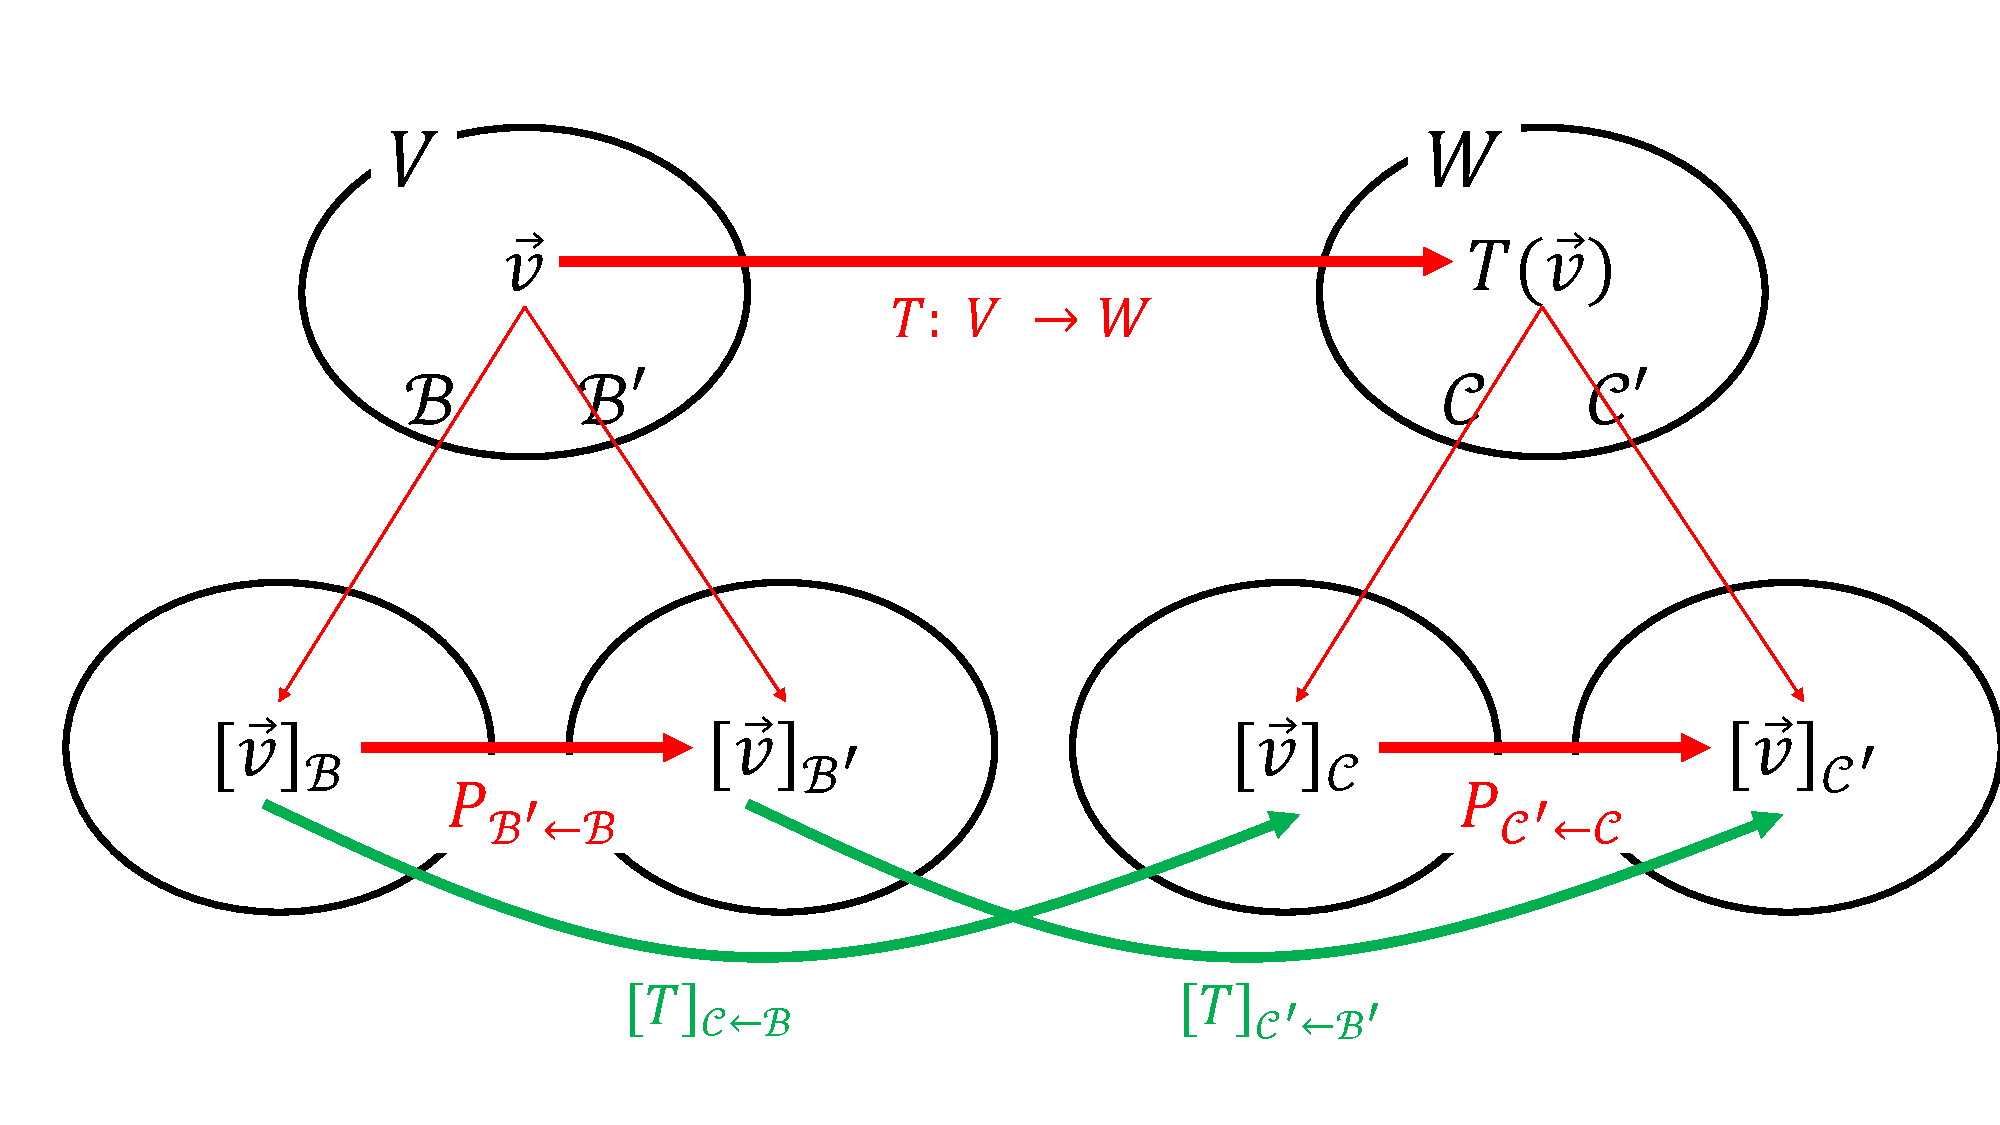
\includegraphics[scale = 0.4]{Figure3.pdf}
	\end{center}
\end{figure} By Theorem 6.12(a) and Theorem 6.12(c), for any vector $\textbf{v} \in V$ and $\textbf{w} \in W$, \begin{align*}
	[\textbf{v}]_{\mathcal{B}} = P_{\mathcal{B} \leftarrow \mathcal{B}'}[\textbf{v}]_{\mathcal{B}'} = \inv{( P_{\mathcal{B}' \leftarrow \mathcal{B}} )}[\textbf{v}]_{\mathcal{B}'}  \mbox{ and } [\textbf{w}]_{\mathcal{C}'} = P_{\mathcal{C}' \leftarrow \mathcal{C}}[\textbf{w}]_\mathcal{C}
\end{align*}
By Theorem 6.26, for every vector $\textbf{v} \in V$, \begin{equation*}
	[T]_{ \mathcal{C} \leftarrow \mathcal{B} }[\textbf{v}]_\mathcal{B} = [T(\textbf{v})]_\mathcal{C} \mbox{ and } [T]_{ \mathcal{C}' \leftarrow \mathcal{B}' }[\textbf{v}]_{\mathcal{B}'} = [T(\textbf{v})]_{\mathcal{C}'}
\end{equation*}
Therefore, for every vector $\textbf{v} \in V$, \begin{align*}
	P_{ \mathcal{C}' \leftarrow \mathcal{C} }[T]_{ \mathcal{C} \leftarrow \mathcal{B} }\inv{(P_{ \mathcal{B}' \leftarrow \mathcal{B}}) }[\textbf{v}]_{\mathcal{B}'} = P_{ \mathcal{C}' \leftarrow \mathcal{C} }[T]_{ \mathcal{C} \leftarrow \mathcal{B} }[\textbf{v}]_\mathcal{B} = P_{ \mathcal{C}' \leftarrow \mathcal{C} }[T(\textbf{v})]_\mathcal{C} = [T(\textbf{v})]_{\mathcal{C}'}
\end{align*}
Since $[T]_{ \mathcal{C}' \leftarrow \mathcal{B}' }$ is the unique matrix satisfying such property (Exercise 6.6 39), this implies that $[T]_{ \mathcal{C}' \leftarrow \mathcal{B}' } = P_{ \mathcal{C}' \leftarrow \mathcal{C} }[T]_{ \mathcal{C} \leftarrow \mathcal{B} }\inv{(P_{ \mathcal{B}' \leftarrow \mathcal{B}}) }$. \\

\textbf{(6.6 45)} \\
Let $\mathcal{B} = \{\textbf{v}_1, \cdots, \textbf{v}_n\}$ be a basis for $V$, and $\mathcal{C} = \{\textbf{w}_1, \cdots, \textbf{w}_m\}$ be a basis for $W$. Let $\Phi: \mathscr{L}(V, W) \rightarrow M_{mn}$ be a transformation defined by \begin{equation*}
	\Phi(T) = [T]_{ \mathcal{C} \leftarrow \mathcal{B} }
\end{equation*} for any linear transformation $T: V \rightarrow W$. \\

(i) For any $S, T \in \mathscr{L}(V, W)$ and any scalar $c$, \begin{align*}
	\Phi(S + T) &= [S + T]_{ \mathcal{C} \leftarrow \mathcal{B} } \\
	&= \begin{bmatrix}
		\left[(S + T)(\textbf{v}_1)\right]_\mathcal{C} & \cdots & \left[(S + T)(\textbf{v}_n)\right]_\mathcal{C}
	\end{bmatrix} \\
	&= \begin{bmatrix}
	\left[S(\textbf{v}_1) + T(\textbf{v}_1)\right]_\mathcal{C} & \cdots & \left[S(\textbf{v}_n) + T(\textbf{v}_n)\right]_\mathcal{C}
	\end{bmatrix} \\
	&= \begin{bmatrix}
	\left[S(\textbf{v}_1)\right]_\mathcal{C} & \cdots & \left[S(\textbf{v}_n)\right]_\mathcal{C}
	\end{bmatrix} + \begin{bmatrix}
	\left[T(\textbf{v}_1)\right]_\mathcal{C} & \cdots & \left[T(\textbf{v}_n)\right]_\mathcal{C}
	\end{bmatrix} \\
	&= [S]_{ \mathcal{C} \leftarrow \mathcal{B} } +  [T]_{ \mathcal{C} \leftarrow \mathcal{B} } = \Phi(S) + \Phi(T) \\
	\Phi(cT) &= [cT]_{ \mathcal{C} \leftarrow \mathcal{B} } \\
	&= \begin{bmatrix}
	\left[(cT)(\textbf{v}_1)\right]_\mathcal{C} & \cdots & \left[(cT)(\textbf{v}_n)\right]_\mathcal{C}
	\end{bmatrix} \\
	&= \begin{bmatrix}
	\left[cT(\textbf{v}_1)\right]_\mathcal{C} & \cdots & \left[cT(\textbf{v}_n)\right]_\mathcal{C}
	\end{bmatrix} \\
	&= c\begin{bmatrix}
	\left[T(\textbf{v}_1)\right]_\mathcal{C} & \cdots & \left[T(\textbf{v}_n)\right]_\mathcal{C}
	\end{bmatrix} = c[T]_{ \mathcal{C} \leftarrow \mathcal{B} } = c\Phi(T)
\end{align*} thus $\Phi$ is a linear transformation. \\

(ii) Let $T_1, T_2 \in \mathscr{L}(V, W)$ such that $\Phi(T_1) = \Phi(T_2)$, then $[T_1]_{ \mathcal{C} \leftarrow \mathcal{B} } = [T_2]_{ \mathcal{C} \leftarrow \mathcal{B} }$. Then for each $i = 1, 2, \cdots, n$, $[T_1(\textbf{v}_i)]_\mathcal{C}$ and $[T_2(\textbf{v}_i)]_\mathcal{C}$ are the same, so $T_1(\textbf{v}_i) = T_2(\textbf{v}_i)$. Let $\textbf{v} \in V$, then there exist scalars $c_1, \cdots, c_n$ such that $\textbf{v} = c_1\textbf{v}_1 + \cdots + c_n\textbf{v}_n$. Then \begin{align*}
	T_1(\textbf{v}) &= T_1(c_1\textbf{v}_1 + \cdots + c_n\textbf{v}_n) \\
	&= c_1T_1(\textbf{v}_1) + \cdots + c_nT_1(\textbf{v}_n) = c_1T_2(\textbf{v}_1) + \cdots + c_nT_2(\textbf{v}_n) \\
	&= T_2(c_1\textbf{v}_1 + \cdots + c_n\textbf{v}_n) = T_2(\textbf{v})
\end{align*} Therefore, $T_1 = T_2$, hence $\Phi$ is one-to-one. \\

(iii) Let $A$ be a $m \times n$ matrix. Let $T: V \rightarrow W$ be a transformation, which is defined by mapping \begin{equation*}
	T(\textbf{v}_i) = A_{1i}\textbf{w}_1 + \cdots + A_{mi}\textbf{w}_m
\end{equation*} for each $i = 1, 2, \cdots, n$, and for any vector $\textbf{v} \in V$, there exist scalars $c_1, \cdots, c_n$ such that $\textbf{v} = c_1\textbf{v}_1 + \cdots + c_n\textbf{v}_n$, then $T(\textbf{v})$ is defined as \begin{equation*}
	T(\textbf{v}) = c_1T(\textbf{v}_1) _+ \cdots + c_nT(\textbf{v}_n)
\end{equation*}
It is trivial from the definition that $T$ is a linear transformation. Also, the definition of $T$ also gives that $[T]_{ \mathcal{C} \leftarrow \mathcal{B} } = A$,  so $\Phi(T) = A$. Therefore, $\Phi$ is onto. \\

By (i), (ii), and (iii), $\Phi$ is an isomorphism, thus $\mathscr{L}(V, W) \cong M_{mn}$. \\

\textbf{(6.6 46)}
Let $n = \dim V$, then $V^\star = \mathscr{L}(V, W) \cong M_{n1}$ by Exercise 6.6 45. Therefore, $\dim V^\star = \dim M_{n1} = n = \dim V$, hence $V^\star \cong V$.
\fi
%\appendix
%\chapter{Cautions on Exam}
\section{Notations}
\begin{table}[h]
	\centering
	\begin{tabular}{|c|c|c|}
		\hline
		Wrong & Right & Explanation \\
		\hline
		$ 2 \cdot 3 = 6 $ & $ 2 \times 3 = 6 $ & \multirow{2}{*}{$ \cdot $ for dot product is only valid for vectors.} \\
		\cline{1-2}
		$ 2 \cdot \textbf{v}$ & $2\textbf{v} $ & \\
		\hline
		$\begin{bmatrix} 1 & 3 & 4 \end{bmatrix}$ & $\begin{bmatrix} 1, & 3, & 4 \end{bmatrix}$ & When writing row vectors, commas are necessary. \\
		\hline
		
	\end{tabular}
\end{table}
\section{Description}
\begin{itemize}
\item Free variables like $s$, $t$ and $u$ must be indicated that they are arbitrary real number. \textit{e.g.} $ s,t \in \mathbb{R} $
%\item Whenever you use FTIM, always start by writing `according to fundamental theorem of invertible matrices' or `가역행렬의 기본정리에 의해'.
\item When proving $ \text{span}\left(\textbf{v}_1,\textbf{v}_2,\textbf{v}_3\right) = \mathbb{R}^{3} $, you must prove each side, not only one.
\item $ A=B $ means not only same entries, but also same size.
%\item Do not write reduced row echelon form as `ref'. This abbreviation is not defined in our book.
\item Write as `적어도 하나는 0이 아닌' instead of `모두 0은 아닌' or else.
\item Abbreviation : only 4 things are allowed : `REF', `RREF', 'EMO', 'F.T.I.M.'. Each of them stands for (Reduced) Row Echelon Form, Elementary Matrix Operation, Fundamental Theorems of Invertible Matrices.
\end{itemize}

\end{document}
